%% Possibly for future editions:

%% More rules for convenience, e.g. defining the \bot symbol, and then
%% defining in and out rules for it

%% Prove that the $\vee$elimination rule is necessary
%% if we didn't have it, then our system would be sound relative to valuations

%% Show that $\phi\vee\bot \equiv \phi$

%% TO DO: synonyms for "entails" or "implies"

%% TO DO: translation from predicate symbols to English

%% TO DO: discuss that "->" may not be truth-functional

%% TO DO: serial relation = entire relation

\documentclass[fleqn]{tufte-book}
\setcounter{secnumdepth}{0}
% \includeonly{rules}
\title{How Logic Works}
\author{Hans Halvorson}
\newcounter{argument}
\newenvironment{argument}{\begin{list}{\arabic{argument}.}{\usecounter{argument}}}{\end{list}}
% \newenvironment{proof}{\begin{eqnarray}}{\end{eqnarray}}
\renewcommand{\theargument}{\arabic{argument}}
\newcommand{\pre}[1]{\item \begin{math} #1\end{math}}
\newcommand{\con}[1]{\item[\copyright] \begin{math} #1 \end{math}}
\newcommand{\ifthen}{\rightarrow}
\newcommand{\qed}{\vdash}
\newcommand{\orr}{\vee}
\newcommand{\andd}{\wedge}
\newcommand{\mitem}[1]{\item \begin{math} #1 \end{math}}
\newcommand{\negg}{\neg}
\newcommand{\bicon}{\leftrightarrow}
\newcommand{\uq}{\forall x}
\newcommand{\eq}{\exists x}
\newcommand{\uqy}{\forall y}
\newcommand{\eqy}{\exists y}
\newcommand{\uqz}{\forall z}
\newcommand{\eqz}{\exists z}
\newcommand{\tr}{\mathrm{T}}
\newcommand{\fa}{\mathrm{F}}
\newcommand{\tfr}{\:\,\vdash\:\,}
\def\ismodeledby{=\joinrel\mathrel|}


\renewcommand{\emph}{\textbf}
\usepackage{xcolor,colortbl}
\definecolor{Gray}{gray}{0.85}
\usepackage[acronym]{glossaries-extra}
\usepackage{svg}
\makeglossaries
\usepackage{venndiagram}
\usepackage{enumitem}
\usepackage{mathtools}
\usepackage{amsthm}
\usepackage{amssymb}
\usepackage{tcolorbox}
\usepackage{multirow}
\newtheorem*{prop*}{Proposition}
\newtheorem{prop}{Proposition}
\numberwithin{prop}{chapter}
\newtheorem*{lemma*}{Lemma}
\newtheorem*{fct}{Finite completeness theorem}
\newtheorem*{dnf}{DNF theorem}
\newtheorem*{subthm}{Substitution theorem}
\newtheorem*{sothm}{Soundness theorem}
\theoremstyle{definition}
\newtheorem*{defn}{Definition}
\newtheorem*{example}{Example}
\newtheorem{exercise}{Exercise}
\newtheorem{exercises}[exercise]{Exercise}
\numberwithin{exercise}{chapter}
% \publisher{Princeton University Press}
\usepackage{array}
\usepackage[caption=false]{subfig}
\usepackage{tikz}
\usetikzlibrary{calc,trees,positioning,arrows,fit,shapes,calc}
\newcommand{\mymk}[1]{%
  \tikz[baseline=(char.base)]\node[anchor=south west, draw,rectangle, rounded corners, inner sep=2pt, minimum size=7mm,
    text height=2mm](char){#1} ;}
\newcommand*\circled[1]{\tikz[baseline=(char.base)]{
            \node[shape=circle,draw,inner sep=2pt] (char) {#1};}}
\usepackage[framemethod=TikZ]{mdframed}
\newcounter{axi}\setcounter{axi}{0}
\renewcommand{\theaxi}{\arabic{axi}}
\newenvironment{law}[2][]{%
    \refstepcounter{axi}
 \ifstrempty{#1}%
% if condition (without title)
{\mdfsetup{%
    frametitle={%
        \tikz[baseline=(current bounding box.east),outer sep=0pt]
        \node[anchor=east,rectangle,fill=blue!20]
        {\strut Axiom~\theaxi};}
    }%
% else condition (with title)
}{\mdfsetup{%
    frametitle={%
        \tikz[baseline=(current bounding box.east),outer sep=0pt]
        \node[anchor=east,rectangle,fill=blue!20]
        {\strut ~#1};}%
    }%
}%
% Both conditions
\mdfsetup{%
    skipabove=2em,
    skipbelow=2em,
    innertopmargin=10pt,linecolor=blue!20,%
    linewidth=2pt,topline=true,%
    frametitleaboveskip=\dimexpr-\ht\strutbox\relax%
}
\begin{mdframed}[]\relax}{%
\end{mdframed}}
\usepackage{tikz-cd}
% \setcounter{secnumdepth}{1}
% \setcounter{tocdepth}{0}
\newcommand{\lra}{\leftrightarrow}

\newtcbox{irule}[1]{coltitle=blue!20!black, colback=black!1!white, 
  colframe=black!10!white,title=#1}

% \tbcset{coltitle=blue!20!black, colback=black!1!white, 
% colframe=black!10!white}

% \tcbset{fonttitle=\bfseries,nobeforeafter,center title}

% \usepackage{imakeidx}

% \makeindex

\tcbuselibrary{skins,xparse}

% \includeonly{models}

\makeglossaries


\doublespacing
\begin{document}
\frontmatter

\maketitle

\tableofcontents

\newglossaryentry{valid}
{
  name={valid},
  description={An argument is valid just in case its premises provide
    decisive support for its conclusion, alternatively, if the truth
    of its premises guarantees the truth of its conclusion} }

\newglossaryentry{atomic sentence} { name={atomic sentence},
  first={\emph{atomic sentence}},
  description={An atomic sentence is a sentence that does not have any
    other sentence as a proper syntactic part.  In propositional
    logic, atomic sentences are represented by capital letters such as
    $P,Q,R,\dots $.  In quantifier logic, the atomic sentences are
    either relation symbols applied to closed terms, such as $Rab$, or equalities between closed terms, such as $a=b$.}
}


\newglossaryentry{interpretation}
{
  name={interpretation},
  description={An interpretation is an assignment of symbols to set-theoretic structures.}
}


\chapter{Preface}

This book has no subject matter --- or, to be more precise, it's about
both everything and nothing.  For the science of logic has no
doctrines or creeds.  There is no set of beliefs that distinguishes
the logical people from the non-logical people, not the beliefs of the
European Enlightenment, nor the deliverances of contemporary natural
science, nor the opinions of some Princeton philosopher.  Simply put,
learning the science of logic can't be reduced to learning any
particular facts at all; it's learning a skill, namely, the skill to
discern between good and bad arguments.

There are numerous reasons why you need this skill, no matter what you
end up doing with your life.  First, being logical will help you
reason about how to get what you want.  Second, many of our society's
best jobs require strong logic skills --- whether it be programming
computers, buying stock options, curing diseases, prosecuting
criminals, discovering alternative energy sources, or interpreting the
constitution.  (And that's not even to speak of that all-important
task of parenting and raising intellectually healthy children.)
Third, regardless of your ideological bent --- whether you're
religious, atheist, or agnostic --- you surely want to do everything
you can to ensure that your view aligns with reality.  For this task,
logic is an invaluable tool, if only to protect you from the plethora
of bad arguments you'll hear in your life.

Our goal here is no more or less than to initiate you into the most
up-to-date account of what makes an argument good.  We'll give you the
tools, but it's up to you to decide how you're going to use them.

\medskip {\it {\bf Note} about how to use this book:} The first six
chapters of this book (up through ``quantifying'') correspond roughly
to a first course in formal logic at an average university in the
United States.  We cover the material in about a quarter of the number
of pages of some well-known logic textbooks, which was intentional:
logic should organize your already existing thoughts, not add to the
jumble of thoughts that need to be organized.

In Chapter 7, we gently ramp up to applications of formal logic, and
in particular to the application of formal logic to the study of
itself (i.e.\ logical metatheory).  In one sense, this material goes
beyond a typical first course in logic, but we would like to change
that.  This material is not intrinsically more difficult than what has
gone before.  In fact, what can make it seem difficult is that it's
less clear what rules of reasoning one is permitted to use.  However,
we try to explain clearly that the rules of reasoning here are none
other than those that were learned in the previous chapters.

Having shown how formal logic can be used to formulate theories, we
then begin to use formal logic to formulate a theory about itself.  In
Chapter 8, we use the theory of sets to define the notion of an
interpretation of a language, and Tarski's rigorous definition of {\it
  truth}.  In Chapter 9, we present a theory about propositional
logic, proving both soundness and completeness theorems.  Finally, in
Chapter 10, we sketch the outlines of a similar theory about
quantifier logic.  Thus, the chapters form a natural staircase leading
up to the treasure-chest of advanced applications of logic, including
modal logic, set theory, and G{\"o}del's theorem.

\medskip {\it {\bf Note} to the instructor, or to the person deciding
  which logic book to use:} To express a thought, or to make an
argument, or to formulate a theory, you have to pick a language to
use.  Similarly, to become more logical, you have to adopt some
particular system of logic.  I've made a choice for you here, and here
is my rationale.

The first choice point is between ``trees'' and ``arguments.''  The
advantage of trees is that they are really easy, and require little
mental exertion.  But wait, isn't the goal to become the most
excellent logical thinkers that we can be?  People don't become better
logical thinkers by being taught a recipe that somebody else found,
and that lets them effectively turn their minds off.  But that's
precisely the point of logical trees: they give students a {\it
  recipe} for evaluating simple arguments.  If the goal were to
manufacture an army of logical automata, then I might well use trees.
But since I'm teaching human beings, I prefer to teach them that
distinctively human skill of making and evaluating arguments.
Accordingly, this book focuses primarily on how to make rigorous
arguments, and secondarily on the (non-algorithmic) skill of detecting
bad arguments.

The second choice point is whether to represent arguments using a
``Fitch-style'' or a ``Lemmon-style'' system.  This is a difficult
decision.  Fitch-style is very intuitive and has a shallow learning
curve.  Unfortunately, Fitch-style argument is opaque to reflection:
it's difficult for students to see why Fitch-style works, and even
more difficult for them to imagine how the rules might have been
different (thereby reinforcing an unfortunate perception that there is
no human creativity involved in formulating the laws of logic).  In
contrast, Lemmon-style argument has a steeper learning curve, but it's
more flexible and transparent to reflection.  It's relatively easy to
see why the system works, and it's easy to tweak the rules and see how
things would come out different.  So, the steeper learning curve of
the Lemmon approach is a price I'm willing to pay to enable my reader
to become a more clear and creative logical thinker.

There are at least three ways in which this book differs from many
other introductory logic books.  First, we teach intrinsic methods
(e.g.\ reasoning) prior to teaching extrinsic methods (e.g.\ checking
with truth tables).  Here our philosophical convictions have been
reinforced by our pedagogical experience, viz.\ that an
argument-centric approach leads to students gaining a higher level of
mastery and confidence, and that the skills gained are more easily
transferable to other intellectual tasks.

Second, and for similar reasons, we treat formal validity as defined
in terms of the inference rules, and not in terms of
truth-preservation.  Our issue here is that a precise notion of
truth-preservation requires a previous understanding of valid
reasoning in set theory.  So, we want to be forthright with our reader
that we, at least, don't have a clear and distinct perception of what
truth-preservation amounts to, at least not until we explicate the
notion in terms of set theory.  By taking formal validity as defined
by the rules, we emphasize that genuine creativity is required to
design rules that both capture and sharpen our intuitions about
validity.

Third, in Chapter \ref{theories}, we ease students away from rigid
formal proofs, and towards ``informal rigor.''  Again, the goal is for
the students to be able to transfer their knowledge to other
disciplines where rigid formal proofs might not be appropriate or
useful.  Fourth, in Chapter \ref{meta}, we introduce logical
metatheory as ``just another theory'' by explaining how to formulate
the metatheory for propositional with predicate logic and a bit of set
theory.  Thus, we close the circle of logic back upon itself.

\medskip {\it {\bf Note} to the reader:} We put an asterisk to the
left of exercises that might be perceived as more difficult than the
preceding ones.  In the case of proofs, it often occurs that a
difficult result is basically a version of the law of excluded middle:
$P\vee \neg P$.  So, if you get stuck, you might try first to prove
excluded middle, and then to use that to get the result you want.

\mainmatter

\newglossaryentry{double turnstile}% label
{
  name={\ensuremath{\vDash}},% default display
  description={semantic implication: whenever the sentences to the
    left of the double turnstile are true, the sentence to the right
    of the double turnstile is true},% description
  category=symbol% category label
}

\newglossaryentry{turnstile}% label
{
  name={\ensuremath{\vdash}},% default display
  description={the relation of provability defined by the inference rules},% description
  category=symbol% category label
} 

\newglossaryentry{main column}
{
  name={main column},
  description={is the column in the truth table of a sentence corresponding to the main connective of that sentence}
}

\newglossaryentry{soundness theorem}
{
  name={main column},
  description={shows that provable sequents are truth-preserving}
} 

\newglossaryentry{substitution instance}
{
  name={substitution instance}, first={\emph{substitution instance}},
  description={A substitution instance of a sentence is any other
    sentence that results from the first by a uniform replacement of
    non-logical terms.  i.e.\ it is any sentence that could result
    from translating that sentence to another language.}
}

\newglossaryentry{main connective} { name={main connective},
  first={\emph{main connective}}, description={for a propositional
    logic sentence $\phi$, the last connective in the construction of
    $\phi$}}

\newglossaryentry{substitution} { name={substitution},
  first={\emph{substitution}}, description={when some non-logical
    symbols are replaced with other suitable syntactic structures}}

\newglossaryentry{subformula} { name={subformula},
  first={\emph{subformula}}, description={a subformula of $\phi$ is
    any formula that occurs in the construction of $\phi$}}

\newglossaryentry{reconstrual} { name={reconstrual}, description={A
    reconstrual assigns non-logical symbols to corresponding syntactic
    structures.  For example, a reconstrual assigns a predicate symbol
    to a formula with one free variable.}  }

\newglossaryentry{dependency number} { name={dependency number},
  first={\emph{dependency number}}, description={a number in the
    leftmost column of a proof that displays which assumptions are in
    force at a particular step in the proof}  }

\newglossaryentry{translation}
{
  name={translation},
  description={A translation is a map from formulas to formulas,
    generated by a reconstrual of the non-logical vocabulary in those formulas.}
}

\newglossaryentry{model}
{
  name={model},
  description={A model of a theory is an interpretation in which all the theory's sentences are true.}
}

\newglossaryentry{sequent}
{
  name={sequent},
  description={A sequent consists of a list of sentences (premises), a
    turnstile $\vdash$, and another sentence (conclusion).  It is the
    symbolic representation of a valid argument form}
}

\newglossaryentry{disjunction}
{
  name={disjunction},
  description={A disjunction is a sentence whose main connective is
    ``or'', symbolized by $\vee$}
}

\newglossaryentry{conditional}
{
  name = {conditional},
  description={A conditional sentence is one whose main connective is
    ``if\dots then'', symbolized by $\to$}
}

\newglossaryentry{extension}
{
  name={extension},
  description={The extension of a relation is the set of things that
    stand in that relation.  The extension of a name is the individual that it denotes}
}

\newglossaryentry{intension}
{
  name={intension},
  description={The intension of a relation is, intuitively, what the relation means}
}

\newglossaryentry{formula}
{
  name={formula},
  description={A formula (alternately, well-formed formula) is a
    string of symbols that could become a sentence by the addition of quantifiers}
}

\newglossaryentry{antecedent}
{
  name={antecedent},
  description={The antecedent of a conditional is the sentence that
    occurs after ``if'', e.g.\ in ``if it is raining then the sidewalk
    is wet,'' the sentence ``it is raining'' is the antecedent}}

\newglossaryentry{consequent}
{
  name={consequent},
  description={The consequent of a conditional is the sentence that
    occurs after ``then'', e.g.\ in ``if it is raining then the sidewalk is
    wet'' the sentence ``the sidewalk is wet'' is the consequent}}

\newglossaryentry{literal}
{
  name={literal},
  description={A propositional logic sentence is called a literal if
    it is atomic or negated atomic}}

\newglossaryentry{truth-functional}
{
  name={truth-functional},
  description={A connective is truth-functional just in case its truth
    value is a function of the truth value of the relevant component
    sentences}}

\newglossaryentry{signature}
{
  name={signature},
  description={A signature is a set of non-logical symbols:
    propositional constants, relation, function, and constant symbols}}

\newglossaryentry{consistent} { name={consistent}, description={A
    collection of sentences is semantically consistent if they can all
    be true simultaneously.  A collection of sentences is
    proof-theoretically consistent if no contradiction can be derived
    from them} }

\newglossaryentry{expressively complete} { name={expressively
    complete}, description={A collection of connectives is
    expressively complete if it can express all truth functions} }

\newglossaryentry{biconditional} { name={biconditional},
  description={A biconditional is a statement of the form ``$\phi$ if
    and only if $\psi$.'' It asserts that $\phi$ is a necessary and
    sufficient condition for $\psi$} }

\newglossaryentry{sufficient condition} { name={sufficient condition},
  description={In a conditional statement ``if $\phi$ then $\psi$'',
    the antecedent $\phi$ is a sufficient condition for $\psi$} }

\newglossaryentry{necessary condition} { name={necessary condition},
  description={In a conditional statement ``if $\phi$ then $\psi$'',
    the consequent $\psi$ is a necessary condition for $\phi$} }

\newglossaryentry{inconsistency} { name={inconsistency},
  description={An inconsistency is a sentence that is false in all
    situations} }

\newglossaryentry{contingency} { name={contingency},
  description={A contingency is a sentence that is true in some
    situations and false in other situations}}

\newglossaryentry{tautology} { name={tautology}, description={A
    tautology is a sentence $\phi$ that is provable from no premises,
    i.e.\ $\vdash \phi$, or that is true merely in virtue of its form,
    or that is true in all situations}}

\newglossaryentry{counterexample}
{
  name={counterexample},
  description={A counterexample to an argument is a formalization of the notion of a situation, or state of affairs,
    in which the premises are true and the conclusion is false.} }

\newglossaryentry{universal quantifier}{ name={universal quantifier},
  first={\emph{universal quantifier}}, description={the symbol
    $\forall$ that plays the role of ``all'' or ``every''}}

\newglossaryentry{existential quantifier}{ name={existential quantifier},
  first={\emph{existential quantifier}}, description={the symbol
    $\exists$ that plays the role of ``some'' or ``there is''}}

\newglossaryentry{variable}{ name={variable}, first={\emph{variable}}, description={a symbol such as $x$, which
    plays the role of an open term}}



\newglossaryentry{dnf}{type=\acronymtype, name={DNF},
  description={disjunctive normal form}, first={\textbf{disjunctive normal
      form (DNF)}}}

\newglossaryentry{cnf}{type=\acronymtype, name={CNF},
  description={conjunctive normal form}, first={\textbf{conjunctive
      normal form (CNF)}}}

\newglossaryentry{em}{type=\acronymtype, name={EM},
  description={law of excluded middle}, first={\textbf{law of excluded
      middle (EM)}}}

\newglossaryentry{raa}{type=\acronymtype, name={RAA},
  description={reductio ad absurdum}, first={\emph{reductio ad
      absurdum (RAA)}}}

\newglossaryentry{dm}{type=\acronymtype, name={DM},
  description={De Morgan's rule}, first={\textbf{DeMorgan's rule (DM)}}}

\newglossaryentry{efq}{type=\acronymtype, name={EFQ},
  description={ex falso quodlibet}, first={\emph{ex falso quodlibet
      (EFQ)}}}

\newglossaryentry{qn}{type=\acronymtype, name={QN},
  description={quantifier negation equivalences},
  first={\emph{quantifier negation equivalences (QN)}}}

\newglossaryentry{complete}{name={complete},
  first={\textbf{completeness}}, description={(1) A complete proof system
    is one the proves everything it should: if $\phi\vDash\psi$ then
    $\phi\vdash\psi$. (2) A theory $T$ is complete just in case
    $T\vdash\phi$ or $T\vdash\neg\phi$, for every sentence $\phi$ in
    its language.}}

\newglossaryentry{sound}{name={sound}, first={\textbf{soundness}},
  description={A sound proof system is one that doesn't prove things
    it shouldn't: if $\phi\vdash\psi$ then $\phi\vDash\psi$.}}

 



\chapter{Logic for Humans}

You're a curious person, I suspect.  You probably already flipped
through the pages of this book, in which case you may have run across
some unfamiliar symbols.  You might have found yourself intrigued ---
like an archaeologist discovering ancient runes.  Or you might have
been put off --- thinking that this book is for quantitative people.

That's what I assumed at first.  I wanted to spend the days of my life
thinking about the big questions of human existence --- what exists,
what we can know, and how we should live.  Calculate the derivative of
a function?  Solve a differential equation?  No thank you.  I'll leave
that to the people who want to build better bridges.  I'd prefer to
move on to the really meaningful and enriching topics.

But I discovered that it's a false dilemma.  In fact, it's not a
dilemma at all.  Symbolic logic is not only for mathematics, and it's
by no means a diversion from the really deep questions of human life.
In fact, symbolic logic represents the best account we have of what it
means to be \textit{rational}.

Although logic is symbolic, it's not really ``mathematical'' in any
sense that puts it in opposition to humanistic endeavors (such as
literature, poetry, history, philosophy, etc.).  Yes, mathematics is a
human activity that displays logical thinking in a particularly clear
way.  But logic itself is involved in any type of human thinking that
aims at finding the truth.  If you've ever argued for a claim, or
evaluated someone else's argument, then you were using logic ---
whether you realized it or not, and whether or not you did a good job
of it.

The goal of this book is simple: it's to make you conscious of how you
already use logic, and thereby to become even better at it.  If you
learn to do symbolic logic, then you will become a better thinker, and
you will understand better what it means to be a good thinker.

\section{Arguments}

Many logic books begin by saying: ``The subject matter of logic is
\dots '' I think these statements are always a bit misleading.  In one
sense, logic doesn't have a subject matter at all.  Logic isn't
\textit{about} something, it's a way of life.

Let's begin by trying to see ourselves from the outside.  Just imagine
that you are an alien who has landed on earth, and you're trying to
understand what human beings are doing when they say that they are
thinking logically.  Imagine that there are two people, say Anne and
Bernt, and that Anne is trying to convince Bernt that something is
true.  Anne might proceed as follows:
\begin{quote}
  Of course gay marriage should be legal.  Only people with some
  backwards religious view would believe otherwise. \end{quote} Here
Anne is trying to convince Bernt that gay marriage should be legal.
But she doesn't try to coerce him with physical force, or even with
intellectual intimidation.  Instead, she offers Bernt a
\textit{reason} why he should accept her conclusion.  To be more
clear, the \emph{conclusion}\index{conclusion} of Anne's argument is
the statement, ``Gay marriage should be legal.''  The reason that Anne
gives for this conclusion --- ``Only people with some backwards
religious view believe otherwise'' --- will be called the
\emph{premise}\index{premise} of the argument.  Thus, the argument
consists of a premise, and a conclusion that is supposed to be
supported by the premise.

Thus, we have three things in play: \emph{argument},
\emph{conclusion}, and \emph{premise}.  The argument itself is made up
of the conclusion and the premise.  The conclusion and premise
themselves are particular sentences.  Notice, moreover, that these
sentences are \textit{assertions}, i.e.\ they make a statement that is
either true or false.  Thus, an argument is built out of assertions
(or statements), some of which are premises, and one of which is the
conclusion.

The key point about an argument is that it's more than just a
disconnected collection of statements.  Suppose that I have ten
notecards, each of which has a statement on it.  If I shuffle them up,
and hand them to you, then I haven't given you an \emph{argument}.
For a collection of statements to be an argument, there has to be some
implied sense in which some of the statements stand in a special
relation to another one of the statements.  In the notecard analogy,
I'd have to hand you a first batch of notecards and say, ``these are
my premises,'' and then I'd have to hand you another notecard and say,
``and this statement is my conclusion --- which, I claim, follows
logically from those premises.''

What is this relation of ``following logically'' that I claim holds
between my premises and my conclusion?  We all know it when we see it,
and we have many words for it --- words such as ``supports'' or
``implies'' or ``entails'' or ``shows that'' or ``grounds''.  That is,
we say things like, ``The fact that there are cookie crumbs on the
carpet \textit{shows that} my son was eating in the living room.''

It's this relation --- whatever it is --- that we really want to
understand.  We want to know: when does this relation hold between
statements?  When does one statement imply another?  There is simply
nothing more basic to human rationality than the notion of one
statement implying another.

We will make a lot of progress in clarifying the notion of
implication.  But we're not going to make progress by means of a
head-on assault.  That is, we're not going to offer you a definition
of the form:
\begin{quote} To say that one statement implies another means that
  \dots \end{quote} Such a definition would be interesting, but it's
not what this book is about.  This book is more of a training manual
for logic connoisseurs.  Just as a wine connoisseur knows a good wine
when he tastes one, so a logic connoisseur knows a good argument when
she sees one.


\section{Logical form}

The study of logic began in ancient Greece --- and possibly in other
places at other times, although that history is less well known to us.
It all began with a single insight, which you've probably already had
yourself.  This insight is that whether or not an argument is good
depends only on its \emph{form}, and not on its \emph{content}.  To
explain this distinction, we need to back up for a second and explain
what we mean by saying that an argument is ``good.''  Consider the
following argument:
\[ \begin{array}{p{7cm}}
  All whales are mammals. \\
  David Hasselhoff is a whale. \\
  Therefore, David Hasselhoff is a mammal. \end{array} \] 
Here there are two premises, and one conclusion.  We've used the word,
``therefore'' to indicate what the conclusion is.  But in truth, the
word ``therefore'' isn't part of the content of the conclusion.  The
conclusion is just the proposition, ``David Hasselhoff is a mammal.''

Is this a good argument?  I hope that your answer is, ``it depends.''
It certainly isn't a perfect argument, because it involves a false
statement, namely that David Hasselhoff is a whale.  Or maybe you don't
know anything about David Hasselhoff?  (Such deplorable lack of
cultural knowledge these days!)  Suppose that David Hasselhoff were
actually a famous whale in a book by an obscure author named Melvin
Hermanville.  In that case --- if Hasselhoff were a whale --- then would
it be a good argument?  Yes, it would definitely be a good argument.

If you're a philosophy type, then you might still be doubtful.  You
might be thinking, ``it all depends on what you mean by `good'.''  If
by ``good'' we mean ``interesting, informative, and non-trivial,''
then that argument might not be very good.  However, logic has no use
for subjective words such as ``interesting.''  Logic is the
\textit{science} of good arguments, and it's interested in isolating
an \textit{objective} sense of goodness in arguments.

The insight --- passed on to us by the ancient Greeks --- is that we
can define ``good argument'' in an objective sense by factorizing
goodness into two distinct pieces.  The first of the two pieces is
easy to understand, but difficult to agree upon in practice: are the
premises true?  The second piece is a bit more elusive, but forms the
subject matter of logic as an objective science: do the premises
support (or imply, or entail) the conclusion?  If the premises do
imply the conclusion, then we say that the argument is valid.
\begin{defn}
  An argument is said to be \emph{\gls{valid}} if its premises imply
  its conclusion. \end{defn} The notion of validity isn't concerned
with whether the premises or conclusion are true or false.  The
question, instead, is a conditional one: \textit{if} the premises were
true, \textit{then} would the conclusion be true?

You should be able to think of cases where you would agree that the
premises support the conclusion, even though you think that the
premises are false.  It might help to use the phrase, ``the premises
\textit{would} support the conclusion'', the idea being that if they
\textit{were} true, then they would imply that the conclusion is also
true.

You should also be able to think of arguments where the premises
\textit{and} conclusion are true, but the premises do \textit{not}
imply the conclusion.  For example, the following is a true premise:
``I love coffee.''  The following is also true: ``I am over six feet
tall.''  But to make an argument from my loving coffee to my above
average height would be patently invalid.  Logical validity is all
about the connection between premises and conclusion; it's not
directly concerned with the question of whether the premises or
conclusion are true.

\section{Sameness of form}

How do we get our hands on this elusive notion of validity, and the
related notion of implication?  Let's begin by looking at obvious
cases --- where an argument is obviously valid, or obviously invalid.
For example, the argument above was obviously valid.  But the argument
below is obviously invalid:
\[ \begin{array}{p{7cm}}
  Princeton is a town in New Jersey.  \\ Therefore, God doesn't
  exist. \end{array} \] Now, you might actually think that both of these
statements are true.  But that most certainly doesn't mean that the
first statement implies the second.  Some true statements just don't
have anything to do with each other.  And that's why this argument is
invalid --- because the premise doesn't give the right kind of support
for the conclusion.

Consider another argument:
\[ \begin{array}{p{7cm}}
  All whales are predators. \\
  Bambi is a whale. \\
  Therefore, Bambi is a predator.
   \end{array} \]
 Is that a valid argument?  Before you answer, remember that validity
 doesn't have anything to do with whether you believe the premises or
 the conclusion.  It's merely a matter of whether there is the right
 kind of connection between premise and conclusion.

  Imagine for a moment that you just learned English, and that you
  aren't yet familiar with the word ``whale,'' or with the name
  ``Bambi.''  For all you know, ``whale'' might mean the same thing as
  ``tiger.''  And for all you know, ``Bambi'' might be the name of a
  tiger at the Philadelphia zoo.

  Here's the amazing thing: you don't have to know anything about the
 meaning of the words ``whale,'' ``predator'' or ``Bambi'' to know
 that this argument is valid.  How do you know it's valid?  I'm not
 going to try to answer that question directly.  I'm going to assume
 that you share my intuition that it is obviously valid.  If you're
 still not convinced, let me put it this way:
 \begin{quote} If all whales were predators, and if Bambi were a
   whale, then would it follow that Bambi is a predator?  \end{quote}
 Now it seems pretty obvious, doesn't it?

 We said that the validity of that argument doesn't depend at all on
 what the ``content words'' mean.  In other words, if an argument is
 valid, then it should remain valid no matter how we interpret the
 content words, or even if we replace the content words with different
 ones.  Thus, given a valid argument (such as the one above), we
 should be able to create a sort of ``mad lib argument'' with
 variables that can be filled in by content words.
 \[ \begin{array}{p{6cm}}
      All $X$ are $Y$.  \\ $m$ is an $X$. \\
      Therefore, $m$ is a $Y$. \end{array} \] 
 No matter what words you put in for $X$, $Y$, and $m$ (provided that
 the result is a well formed sentence), you get a valid argument.

 The thing above with the variables, it's like a blueprint for
 constructing arguments.  Choose some content words, plug them in, and
 ta da, you have a valid argument.  Let's call it an \emph{argument
   form}.  In this case, it's a valid argument form, because no matter
 what words you plug in, the argument comes out as valid.

 But how did we know that those arguments were valid in the first
 place?  To be honest, it's just our intuition that tells us that
 these arguments are valid.  Nobody found a tablet of stone on a
 mountain with the argument form above.  Instead, that argument form
 was written down by a human being in an effort to capture what is
 common in a bunch of arguments that we feel (intuitively) to be
 valid.

 That's how we'll proceed in the first part of this book: we will
 collect several basic argument forms that seem obviously valid.  Then
 we'll learn how to string valid argument forms together to create
 longer valid arguments.

%%% Local Variables:
%%% mode: latex
%%% TeX-master: "main"
%%% End:


\chapter{Deducing} \label{deduce}

Let's look at another obviously valid argument.
\[ \begin{array}{p{6cm}} Roses are red and violets are blue. \\ \hline
    Roses are red. \end{array} \] (Here the horizontal line functions
as a ``therefore'' indicator.)  The reason this argument is valid is
because the conclusion just extracts one of two sentences that are
conjoined in the premise.  In other words, the argument form looks
like this:
\[ \begin{array}{p{1.7cm}} 
  $P$ and $Q$ \\ \hline $P$ \end{array} \] Here we've replaced
``roses are red'' with the letter $P$, and we've replaced ``violets
are blue'' with the letter $Q$.  Obviously, the argument would be
valid no matter what sentences we put in for $P$ and $Q$.

\newglossaryentry{conjunction}
{
  name=conjunction,
  description={a conjunction is a formula that is built from two other formulas,
    using the connective $\wedge$}
} 

The reason why this argument form is valid is because of the way that
the word ``and'' works.  It's a special word that connects two
statements into one bigger statement that logically implies both of
the original statements.  Since ``and'' plays this special logical
role, it can be helpful to make it stand out.  We'll use the symbol
``$\wedge$'' as shorthand for ``and,'' so that ``$P\wedge Q$'' will
stand for ``$P$ and $Q$.'' In this case, the argument form above looks
like this:
\[ \begin{array}{c} P\wedge Q \\ \hline P \end{array} \] Our arguments
are gradually changing from linguistic to symbolic --- but simply
because we're trying to capture the essence of what makes them valid.
The symbol $\wedge$ here is not a new thing.  It's just the good old
notion of ``and'', written in compact notation.  And that will be the
case for \textit{everything} you encounter in this book.  In this
book, we won't need to introduce new things that you've never
encountered before in your life.  In this way, logic is quite
different from empirical sciences such as biology, chemistry, or
physics.  In physics, you'll run into things like ``quantum fields,''
which I imagine your mother didn't tell you about.  But in logic,
we're just going to make precise concepts that you use already in
everyday life.

\tcbset{enhanced,colback=white,coltitle=black,colbacktitle=white,fonttitle=\bfseries,sharp
corners}

\bigskip
\begin{tcolorbox}[enhanced,width=10cm,title=conjunction elimination
  ($\wedge$E),attach boxed title to top
  left={yshift=-2mm,xshift=4mm},boxed title style={sharp corners}] For
  any two sentences $\phi$ and $\psi$, you are permitted to infer both
  $\phi$ and $\psi$ individually from the conjunction
  $\phi\wedge \psi$. \end{tcolorbox}

\bigskip 

The Greek letters $\phi$ and $\psi$ here are meant to emphasize the
schematic nature of inference rules.  In particular, a Greek letter
like $\phi$ can stand for any sentence whatsoever, whether it be $P$
or $Q$ or $P\wedge Q$ or $P\wedge (P\wedge Q)$.  So, for example,
$\wedge$E allows one to infer $P$ from $P\wedge Q$, and it also allows
one to infer $(Q\wedge P)$ from $(Q\wedge P)\wedge
Q$. \index{conjunction}

In practice, we use the rules (such as $\wedge$ elimination) in a
linear format, moving from the top of the page to the bottom.  For
example, the following is a typical application of $\wedge$
elimination.
\[ \begin{array}{l >{$}p{2cm}<{$} p{1.5cm}}
      (1) & P\wedge Q & A \\
      (2) & P & 1 $\wedge$E
   \end{array} \]
 Here the first line is annotated with ``A,'' which means that it's
 an assumption of the problem.\footnote{In this chapter, assumptions
   are things that are given to you --- as part of the problem you're
   trying to solve.  In the next chapter, we'll
   explain how you can make your own assumptions.}  The second line is annotated with ``1
 $\wedge$E,'' which means that the conjunction elimination rule was used on line
 $1$.  In a correctly written (i.e.\ valid) proof, every line
 must either be an assumption, or it must be justified by one of the
 rules of inference.

Here's a slightly more complicated proof of $P$ from \mbox{$(P\wedge
Q)\wedge (R\wedge P)$}.
\[ \begin{array}{l >{$}p{3cm}<{$} p{1.5cm}}
      (1) & (P\wedge Q)\wedge (R\wedge P) & A \\
     (2) & P\wedge Q & 1 $\wedge$E \\
     (3) & P    & 2 $\wedge$E 
   \end{array} \]
 Note that we weren't forced to take the route that we did.  We could
 have peeled off the conjunct $R\wedge P$ instead, and used that to get
 $P$.  In fact, logic never tells you what steps you must take; it only
 tells you what steps you are permitted to take.  It's up to you to decide
 where you want to go and how you want to get there.
 
Just as a conjunction can be disassembled into its conjuncts, so a
conjunction can be assembled from individual propositions.  So we have
a rule:

\bigskip
\begin{tcolorbox}[enhanced,width=10cm,title=conjunction introduction
  ($\wedge$I),attach boxed title to top
  left={yshift=-2mm,xshift=4mm},boxed title style={sharp corners}]
  For any two sentences $\phi$ and $\psi$, you are permitted to infer
  $\phi\wedge \psi$ if you already have both $\phi$ and
  $\psi$. \newline 
  Schematically: $\begin{array}{c c}
       \phi \qquad  \psi \\ \hline
       \phi \wedge \psi \end{array} $ \end{tcolorbox}

\bigskip 

So, when you use conjunction introduction, you will cite two lines, one for
each conjunct.  For example: \[ \begin{array}{l >{$}p{2.5cm}<{$} p{1.5cm}}
                    (1) & P & A   \\
                    (2) & Q & A   \\
                    (3) & P\wedge Q & 1,2 $\wedge$I
                                \end{array} \]
Note, however, that you can use the same line twice.  For example, the
following counts as a valid application of conjunction introduction:
\[ \begin{array}{l >{$}p{2.5cm}<{$} p{1.5cm}}
     (1) & P  & A   \\
     (2) & P\wedge P & 1,1
                       $\wedge$I \end{array} \] It also doesn't matter
 which order the lines occur in.  For example, if $Q$ occurs before $P$, then you can use conjunction introduction to infer either $Q\wedge P$ or $P\wedge Q$.
                                   
At this stage, we need to introduce another device.  Suppose that you
already have one conjunction, say $P\wedge Q$, and you want to
conjoin it with yet another statement, say $R$.  In that case, to
conjoin the first composite statement with the second simple
statement, you first have to put the first sentence into parentheses,
as follows:
  \[ \begin{array}{l >{$}p{2.5cm}<{$} p{1.5cm}}
      (1) & P\wedge Q & A    \\
       (2) & R  & A  \\
       (3) & (P\wedge Q)\wedge R &  1,2 $\wedge$I \end{array} \]
You might be thinking that these parentheses aren't really necessary,
because it doesn't matter which conjunction gets put in first.  There
is a sense in which that is correct.  But for now, let's be careful to
keep track of where things are coming from.

\newglossaryentry{conjunct}
{
  name=conjunct,
  description={a conjunct is one of the two subformulas that are combined with
    $\wedge$ to form a conjunction}
}

It's also crucial to note that this rule is schematic.  In particular,
$\wedge$ elimination allows you to derive a \gls{conjunct} from any
conjunction, e.g.\ both $P$ and $Q\wedge R$ may be derived from
$P\wedge (Q\wedge R)$.  Note, however, that $\wedge$E does
\textit{not} allow you to derive $Q$ immediately from
$P\wedge (Q\wedge R)$, because the original sentence isn't a
conjunction of $Q$ with something else.  Each conjunctive sentence has
precisely two conjuncts.  In this case, the two conjuncts are $P$ and
$Q\wedge R$.  The latter is a conjunction, so that the sentence $Q$ is
``two levels deep'' inside the conjunction $P\wedge (Q\wedge R)$.
We'll explain this notion of ``levels'' inside sentences in Chapter
\ref{meta}.  But for now, your intuitions should suffice to keep you
out of trouble.

With these two rules ($\wedge$E and $\wedge$I), you can now start
proving some stuff on your own.

\begin{exercises} \mbox{}
  \begin{enumerate}
  \item Prove that $Q\wedge P$ follows from $P\wedge Q$.  That is,
    write $P\wedge Q$ on line $(1)$, then use the rules ($\wedge$
    introduction and elimination) repeatedly until you obtain
    $Q\wedge P$.
  \item Prove that $P\wedge (Q\wedge R)$ follows from
    $(P\wedge Q)\wedge R$.
    \end{enumerate}
\end{exercises}

In this book, if a concept is really important, then we'll probably
invent a symbol for it.  The reason we do that is because it makes it
easy for us to identify instances where that concept is being used.
The most important concept in this book is the concept of a
\emph{valid argument} (and the related concepts of when one statement
\emph{entails} or \emph{implies} another statement).  Since this
concept is so central to this book, we'll give it a symbol
$\gls{turnstile}$.  Thus, we write $P\wedge Q\vdash P$ as shorthand
for ``$P\wedge Q$ logically implies $P$''.  Or, to be even more
precise, $P\wedge Q\vdash P$ means that there is a correctly written
proof that begins with $P\wedge Q$ and that ends with $P$.  The entire
string $P\wedge Q\vdash P$ is called a \emph{\gls{sequent}}, which is
just a fancy name for a logically valid argument in our symbolic
language. \index{sequent}

The most general sequent then looks something like this:
\[ \phi _1,\dots ,\phi _n\: \vdash \:\psi \] which says that there is
a proof that assumes $\phi _1,\dots ,\phi _n$ are derives $\psi$.  For
example, using conjunction introduction, you can easily write a
three-line proof that establishes the sequent $P,Q\vdash P\wedge Q$.
Another four-line proof with conjunction introduction establishes the
sequent $P,Q\vdash P\wedge (P\wedge Q)$.

To keep your head clear, it's best not to think of sequents like
$\phi\vdash\psi$ as sentences of the artificial language we're
describing.  Imagine that we're designing an artificial intelligence,
and we're programming it with rules for drawing valid inferences.  In
this case, ``$P$'' and ``$Q$'' are sentences of the AI's language, and
$\wedge$ is a connective that can be used to build more and more
complex sentences in the AI's language.  However, the symbol $\vdash$
is not of the same kind.  It's not part of the AI's language, but part
of our design language --- which we use to describe the permissible
reasoning processes for the AI.  In particular, $\phi\vdash\psi$ means
that the AI can --- by using the rules we've specified --- derive
$\psi$ from $\phi$.  But $\phi\vdash\psi$ is not itself one of the
sentences that the AI is programmed to assert.

By stating the rules (such as $\wedge$I and $\wedge$E), we are
gradually building up the relation $\vdash$ that holds between
premises and conclusions.  We want to build up slowly and carefully so
that we don't by accident declare that an argument is valid when, as a
matter of fact, it's not really valid.

At the moment, we have only two rules.  Now it's time to add some
more.  Let's start with a rule for introducing disjunctions, that is
sentences that involve an ``either \dots or \dots '' clause, which
we'll abbreviate by the symbol ``$\vee$''.  That is, we'll symbolize
``either $P$ or $Q$'' as \mbox{``$P\vee Q$''}. \index{disjunction}

Before we state the disjunction introduction rule, note that there are
two ways that we use disjunctions in English.  In one sense, a
\gls{disjunction} presents you with \textit{exclusive} choices.  For
example, a person can be born either in the US or in the UK (but of
course a person cannot be born in both places).  In another sense, a
disjunction just tells us that at least one of the two options holds.
For example, a person can be either a US citizen or a UK citizen ---
and, as a matter of fact, it's possible to be both.  In this case, the
disjunction is \textit{inclusive}.

If we take disjunction in the inclusive sense, then a disjunction
always follows from either one of its disjuncts.  For example, if I
tell you that I'm a US citizen, then you know that I'm either a US
citizen or a UK citizen.  You might not typically have any need to
draw such an inference --- once you know that one of the disjuncts is
true, why would you bother to assert the disjunction?  In real life,
asserting a disjunction is most useful when you have reason to think
that one of the two disjuncts must be true, but you don't know which
one.  For example, you know that I'm either a US citizen, or I'm not a
US citizen, even if you don't know which of those two is the case.

We hereby stipulate that $\vee$ will behave like inclusive
disjunction, and hence the following rule makes sense.

\bigskip
\begin{tcolorbox}[enhanced,width=10cm,title=disjunction introduction
  ($\vee$I),attach boxed title to top
  left={yshift=-2mm,xshift=4mm},boxed title style={sharp corners}]
  Given $\phi$, you are permitted to infer \mbox{$\phi\vee \psi$}, for
  any sentence $\psi$ whatsoever.  Similarly, given $\phi$, you are
  permitted to infer \mbox{$\psi\vee\phi$}, for any sentence $\psi$
  whatsoever.  Schematically:
  $ \begin{array}{c p{0.1cm} c}
       \phi & & \phi \\ \cline{1-1} \cline{3-3} 
    \phi \vee \psi & & \psi\vee\phi \end{array} $ \end{tcolorbox}

\bigskip 

The funny thing about disjunction introduction is that it throws
information away.  From a stronger premise $P$, you get to infer a
weaker conclusion $P\vee Q$.  Why would anyone ever want to do that?
In short, weakening premises becomes really useful in contexts where
two different premises lead to the same weakening.  But we'll get to
that maneuver later, in the next chapter.  For now, we can start using
disjunction introduction in combination with our conjunction rules.
\[ \begin{array}{l >{$}p{3.25cm}<{$} p{2cm}}
     (1) & P\wedge Q & A \\
     (2) & P         & 1 $\wedge$E \\
     (3) & P\vee R   & 2 $\vee$I \\
     (4) & Q         & 1 $\wedge$E \\
     (5) & R\vee Q   & 4 $\vee$I \\
     (6) & (P\vee R)\wedge (R\vee Q) & 3,5 $\wedge$I \end{array}\]
Notice how we disjoin $R$ on the right in line 3, and on the left in
line 5.  The disjunction introduction rule allows both of these moves.

Keep in mind that disjunction introduction allows you to disjoin anything you
want.  So, for example, the following is also valid.
\[ \begin{array}{l >{$}p{1.75cm}<{$} p{2cm}}
     (1) & P & A \\
     (2) & P\vee P & 1
                     $\vee$I \end{array} \] The disjunction
 introduction rule might seem too liberal, because the premise $\phi$
 puts no constraints on the statement $\psi$ that occurs in the
 conclusion $\phi\vee\psi$.  For example, the following argument is
 valid.
 \begin{quote} Klaas is a professor. \newline Therefore, either Klaas
   is a professor or he is a serial killer.  \end{quote} If it seems
 strange to you that this argument is valid, then I suspect it is
 because we usually have no good reason to assert a disjunction when
 we're already in a position to assert one of the disjuncts.  For
 example, if you told somebody (who doesn't know Klaas) that Klaas is
 either a professor or a serial killer, then they are likely to infer
 that you are unsure which he is --- and, that if you were shown
 evidence that Klaas is not a professor, then you would conclude that
 he is a serial killer.  But logically speaking, those inferences are
 not warranted.  If you are shown evidence that Klaas is not a
 professor, when you previously believed that he is, then you're more
 likely to retract the claim that Klaas is either a professor or a
 serial killer.
 
It's time then that we further clarified our methodology.  Our aim
here is \textit{not} to capture every single intuition we might have
about good arguments that are stated in our natural languages.
Instead, our aim is to find the best \textit{formal} model of the
notion of validity.  And the thing about formal models is that they
can have two distinct types of virtues.  On the one hand, it's good to
fit the facts (in this case, our intuitions about which arguments are
valid).  On the other hand, it's good for our formal apparatus to be
be both powerful and manageable.  It might be helpful to think of an
analogy here.  Think of how physics describes the motion of
projectiles.  One of the first things that a physicist does is to make
some idealizing assumptions, e.g.\ that there is no wind resistance.
That assumption won't really hold in real-life applications.  But
making such an idealizing assumption allows a physicist to bring to
bear the powers of abstract reasoning to figure out a lot of
information that will be approximately true in many different
situations.

Here's another way of putting the same thing.  The physicist's model
of projectile motion is an \textit{analogy} for projectile motion in
the real world.  In the same way, symbolic logic is supposed to be an
analogy for good arguments in real life.  As with any analogy, it
breaks down at some point --- in this case, it already breaks down in
the failure of the logical $\vee$ to capture all the nuances of the
natural language ``or.''  However, this disanalogy is the price of
constructing a system that is powerful, manageable, and applicable in
many different situations in life.

\begin{exercises} Prove the following sequents.
  \begin{enumerate}
  \item $P\wedge Q\:\vdash\:Q\vee R$
  \item $P\wedge Q\:\vdash (P\vee R)\wedge (Q\vee R)$  
  \item $P\:\vdash\:Q\vee (P\vee Q)$
  \item $P\:\vdash\: (P\vee R)\wedge (P\vee Q)$
  \end{enumerate}
\end{exercises}

So far we've found two special logical words that enable valid
inferences: ``and'' and ``or''.  Are there any other logical words
besides them?  Yes, there are many others.  The next one we'll look at
is ``if $\phi$ then $\psi$'', which we symbolize as ``$\phi\to\psi$''.
The sentence $\phi\to\psi$ is called a \emph{\gls{conditional}}; the
first component sentence $\phi$ is its \emph{\gls{antecedent}}, and
the second component sentence $\psi$ is the \emph{\gls{consequent}}.

The statement $\phi\to\psi$ does not, by itself, imply either $\phi$
or $\psi$.  It only tells us that, in combination with $\phi$, you're
entitled to conclude that $\psi$.  Thus, the rule for eliminating
$\to$ requires a second premise as follows:
\bigskip 
\begin{tcolorbox}[enhanced,width=10cm,title=modus ponens (MP),attach boxed title to top
  left={yshift=-2mm,xshift=4mm},boxed title style={sharp corners}]
Given \mbox{$\phi\to\psi$} and $\phi$, you are permitted to conclude $\psi$.
Schematically: $\begin{array}{c} \phi\to \psi \quad \phi \\ \hline
    \psi \end{array}$ \end{tcolorbox} \bigskip By our earlier
convention, we should call this rule ``$\to$ elimination.'' However,
it has an old Latin name \emph{modus ponens}, and we'll follow
historical precedent.
 
As with our previous inference rules, MP is implicitly schematic.
That is, it doesn't apply only to the specific conditional $P\to Q$,
it applies to any conditional, such as $(P\vee Q)\to R$.  For example,
we can use MP now to derive $R$ from $(P\vee Q)\to R$ and $P$.
\[ \begin{array}{l >{$}p{3cm}<{$} p{2cm}}
     (1) & (P\vee Q)\to R & A  \\
     (2) & P    & A  \\
     (3) & P\vee Q & 2 $\vee$I  \\
     (4) & R & 1,3 MP \end{array} \] Notice how we used
MP on a conditional (line 1) whose antecedent is complex (a
disjunction $P\vee Q$).
That's perfectly OK, because MP is schematic.  In other words, MP
works on any conditional sentence, no matter whether its antecedent
and consequent are simple or complex.  You have to be careful,
however, only to apply inference rules to an entire line.  For
example, you cannot apply MP to the sentences $P\vee (Q\to R)$ and
$Q$, because the first sentence is a disjunction, not a conditional.

Sometimes one conditional is embedded in another, as for example if I
say, ``if you take my class, then if you do the homework you will
learn some logic.''  In such cases, we might have to apply MP twice
to detach the consequent of the conditional.  Here then is a
derivation of $R$ from the premises $P\to (Q\to R)$ and $P\wedge Q$.
\[ \begin{array}{l >{$}p{3cm}<{$} p{2cm}}
     (1) & P\to (Q\to R) & A \\
     (2) & P\wedge Q     & A \\
     (3) & P             & 2 $\wedge$E \\
     (4) & Q\to R        & 1,3 MP \\
     (5) & Q             & 2 $\wedge$E \\
     (6) & R             & 4,5 MP \end{array} \]
Again, you have to be careful only to apply MP when the main
sentence on a line is a conditional, and you also have the antecedent
of that conditional.  For example, given premises $(P\to Q)\to R$ and
$P$ you should {\it not} infer that $Q$, or that $Q\to R$.  While
$(P\to Q)\to R$ is a conditional, its antecedent is $P\to Q$.

\begin{exercise} Prove that the following argument forms are valid.
  You may use the rules $\wedge$E, $\wedge$I, $\vee$I, and MP.
  \begin{enumerate}
\item $P\ifthen (Q\ifthen R),\,P\ifthen Q,\,P\:\vdash\: R$
% 4; MT, DN
\item $(A\orr B)\ifthen T,\,Z\ifthen A,\,T\ifthen W,\,Z\:\vdash\:W$
% 8; &E, MT, MP, vI
\item $(A\ifthen  B)\andd (C\ifthen A),\,(C\andd (W\ifthen  Z))\andd W\:\vdash\:(B\orr D)\andd  (Z\orr E)$
\item $P\to (P\to Q),\,P\:\vdash\: Q$
\item $P\wedge (P\to Q)\:\vdash\: P\wedge Q$  
\end{enumerate} \end{exercise}

Our brains are so accustomed to using modus ponens that we sometimes
make the simple mistake of trying to apply it in the opposite
direction.  For example, I've heard more than one person put
forward the following argument.
\[ \begin{array}{p{8cm}}
     If God exists then there are objective moral rules. \\
     There are objective moral rules. \\ \hline
     God  exists. \end{array} \]
 This argument has the form:
 \[ \begin{array}{l}
      P\to Q \\
      Q \\ \hline
      P \end{array} \]
which is like backwards modus ponens, since the consequent is the
premise, and the antecedent is the conclusion.  However, this argument
form is invalid.  Consider, for example, the following instance
of the same form.
\[ \begin{array}{p{8.5cm}}
  If UCLA is in Palo Alto, then UCLA is in California. \\
  UCLA is in California. \\ \hline
  UCLA is in Palo Alto.  \end{array} \]  This argument has obviously
true premises, and an obviously false conclusion.  Therefore it's
invalid, and its form doesn't guarantee validity.  

In general, if an argument form is \emph{invalid}, then it admits some
instance where the premises are true and the conclusion is false.
This instance is called a \emph{\gls{counterexample}} to the argument
form.  Historically, invalid argument forms have often been called
\emph{fallacies}, especially when people commonly mistake the form for
valid.  The previous example is in instance of the fallacy of
\emph{affirming the consequent}.

\section{Negation}

We turn now to negative phrases, such as ``it is not the case that
\dots '', which we'll symbolize with $\neg$.  That is, we write ``it
is not the case that $P$'' as $\neg P$.  With this new connective in
hand, we can capture another valid argument form using the ``if \dots
then '' connective.  Consider, for example, the following argument:
\[ \begin{array}{p{6cm}}
  If $n$ is divisible by $4$, then $n$ is even.      \\ 
  $n$ is not even.       \\ \hline 
  $n$ is not divisible by $4$.     \end{array} \]
This argument is valid, and it's an instance of a famous argument
form.

\bigskip 
\begin{tcolorbox}[enhanced,width=10cm,title=modus tollens (MT),attach boxed title to top
  left={yshift=-2mm,xshift=4mm},boxed title style={sharp corners}]
   Given $\phi\to \psi$ and $\neg \psi$, you are permitted to infer $\neg
  \phi$.  \newline Schematically: $\begin{array}{c c}
       \phi\to \psi \quad \neg\psi \\ \hline
       \neg\phi \end{array} $
   \end{tcolorbox}
\bigskip 


% \begin{law}[Modus Tollendo Tollens (MT)]{}
%   Given $P\to Q$ and $\neg Q$, you are permitted to infer $\neg
%   P$. Schematically:
%   \[ \begin{array}{c c}
%        P\to Q \quad \neg Q \\ \hline
%        \neg P \end{array} \] \end{law}
As with MP, the new rule applies not just to the conditional sentence
$P\to Q$, but to any other conditional, such as $(P\wedge Q)\to R$ or
$P\to (Q\wedge \neg Q)$.

%% TO DO: Necessary and sufficient conditions
%% "only if" "unless"

\begin{exercise} Prove that
  $Q\to (P\to R),\,\neg R\wedge Q\:\vdash\: \neg P$.
\end{exercise}

Modus ponens can be restated as follows: a conditional $\phi\to \psi$
says that the antecedent $\phi$ is a \emph{\gls{sufficient condition}}
for the consequent $\psi$.  In other words, the truth of $\phi$ is a
guarantee of the truth of $\psi$.  Modus tollens can then be restated
as: a conditional $\phi\to \psi$ says that the consequent $\psi$ is a
\emph{\gls{necessary condition}} for the antecedent $\phi$.  In other
words, the falsity of $\psi$ is a guarantee of the falsity of $\phi$.
To understand the difference between necessary and sufficient
conditions, think about the example of rain and clouds.  To say that
rain is a sufficient condition for clouds does not mean that rain
causes clouds, but merely that the truth of ``it's raining''
guarantees the truth of ``there are clouds''.  To say that clouds are
a necessary condition for rain means that the falsity of ``there are
clouds'' guarantees the falsity of ``it is raining''.

It's important also to be totally clear about the relation between the
phrase ``\dots if \dots'' and the phrase ``\dots only if \dots
.''  Consider the following examples.
\begin{enumerate}
  \item Alice is admitted to Harvard medical school only if she has a high
  MCAT score.
  \item Alice is admitted to Harvard medical school if she has a high
    MCAT score.
  \end{enumerate}
  The first sentence says that having a high MCAT score is a necessary
  condition for Alice being admitted.  The second sentence says that
  having a high MCAT score is a sufficient condition for Alice being
  admitted.  I would guess that the first sentence is true, no matter
  who Alice is, and that the second sentence is usually false ---
  because having a high MCAT score is not a sufficient condition for
  admission to the best medical schools.
 
To get the full effect out of modus tollens, we need to say something
more about the logical role of negation.  It turns out that the role
of negation is a bit more controversial than you might have thought.
But as this is an introductory book, we're going to begin with a
simplistic picture of negation.

When I was young, I was taught that it's bad English to use double
negations, such as ``you don't know nothing.''  My mother told me that
that sentence really means that you do know something, and so I should
say ``you don't know anything.''  Now, the goal of this book isn't to
teach you to speak better English; and being a living and growing
language, English has an enormous amount of subtlety in expression.
In particular, two negatives in English don't always mean exactly the
same thing as a positive.  In contrast, our symbolic language is
extremely literal and rigid.  We will stipulate in fact that two
negations is logically equivalent to no negation at all.

\bigskip 
\begin{tcolorbox}[enhanced,width=10cm,title=double negation (DN),attach boxed title to top
  left={yshift=-2mm,xshift=4mm},boxed title style={sharp corners}]
Given $\phi$ you are permitted to infer $\neg \neg \phi$, and given
$\neg \neg \phi$ you are permitted to infer $\phi$. \newline Schematically:
  $\begin{array}{c c c} \begin{array}{c} \phi \\ \hline \neg\neg
        \phi \end{array} & & \begin{array}{c} \neg \neg \phi \\ \hline
        \phi \end{array} \end{array} $
\end{tcolorbox}
\bigskip 

Among logicians, mathematicians, and philosophers, there has been some
skirmishing about whether the second of these rules (i.e.\ the DN
elimination rule) is valid.  The thought was: how can proving that
something is not true establish that something is true?  The foes of
DN elimination are typically called {\it intuitionists}, after an
early twentieth-century movement in the philosophy of mathematics.
However, our methodology in this book is more empiricist than it is
rationalist.  In particular, we're not going to stop and search for
some Platonic insight into whether or not the rules are valid.
Instead, we'll accept the rules as tentative conventions, and then
we'll explore their consequences.  We believe it's good to ask the
deep philosophical question about which are the right rules --- but it
can be good to keep that question on the back-burner while you're
figuring out the consequences of the rules.

As with the other connective symbols, the negation symbol can be
applied repeatedly.  For example, we can have $\neg P$ or $\neg\neg P$
or $\neg\neg\neg P$, etc.  Of course, DN elimination can be applied
whenever there are two or more negation symbols, and it allows us to
remove the first two.  For example, the following is a valid
inference:
\[ \begin{array}{l >{$}p{1.5cm}<{$} p{2cm}}
     (1) & \neg\neg\neg P & A \\
     (2) & \neg P & 1 DN \end{array} \] It can also make a big
 difference which order the connectives are applied.  So, for example, $\neg (P\to Q)$ says something very different than $\neg P\to Q$.  (The former is a negated sentence, and the latter is a conditional.)  We take the negation sign to apply only to what comes immediately after it.  So, in the sentence $\neg P\to Q$, the negation applies only to $P$.  In $\neg (P\to Q)$, the negation applies to $P\to Q$.  Be careful only to use DN when the entire sentence on a line is negated twice.  For example, the sentence $\neg (\neg P\to Q)$ is {\it not} a candidate for DN elimination, because the first negation symbol applies to the conditional $\neg P\to Q$, and not to the negation $\neg P$.  Similarly, you are not permitted to apply DN introduction to a subformula.  For example, you may not use DN to infer $\neg\neg P\to Q$ from $P\to Q$, because the former sentence is a conditional, not a twice-negated sentence.\footnote{Later we will show that any subformula $\phi$ can in fact be replaced by $\neg\neg\phi$. See page \pageref{replacement}. But we we want to start with a small number of strict rules, and then do some work to show that these rules allow us to prove a lot of interesting things.}

We can now use all of our deduction rules in combination to prove
further validities, such
as $P\to\neg Q,Q\vdash \neg P$.
\[ \begin{array}{l >{$}p{2cm}<{$} p{2cm}}
     (1) & P\to \neg Q    & A \\
     (2) & Q              & A \\
     (3) & \neg \neg Q    & 2 DN \\
     (4) & \neg P         & 1,3 MT \end{array} \]
Notice that we needed to infer line $3$ before using MT, 
because $Q$ is not itself literally the negation of $\neg Q$. In
formal logic, there are no shortcuts; the rules must be applied
exactly as they are stated.

The following more complicated proof shows that $\neg P$ follows from
$\neg (P\to Q)\to Q$ and $\neg Q$.
\[ \begin{array}{l >{$}p{3cm}<{$} p{2cm}}
     (1) & \neg (P\to Q)\to Q  & A \\
     (2) & \neg Q              & A \\
     (3) & \neg\neg (P\to Q)   & 1,2 MT \\
     (4) & P\to Q              & 3 DN \\
     (5) & \neg P              & 4,2 MT 
   \end{array} \]
Here we used $\neg Q$ twice over: once to get $\neg\neg (P\to Q)$, and
once to get $\neg P$.

\section{Equivalence}

You'll have noticed that some proofs go both ways.  For example, you
can prove $Q\wedge P$ from $P\wedge Q$, and vice versa.  In this case,
we'll write $P\wedge Q\dashv\vdash Q\wedge P$, indicating proofs in
both directions, and we'll say that the two sentences are
\emph{provably equivalent}.  There is a strong sense in which provably
equivalent sentences are the same ``for all logical purposes''.

\begin{exercise} Prove the following sequents.
  \begin{enumerate} \item $P\wedge (Q\wedge R)\:\dashv\vdash\:
  (P\wedge Q)\wedge R$ \item $P\:\dashv\vdash\: P\wedge
  P$ \end{enumerate} \end{exercise}

\section{Summary}

In this chapter, we identified some particularly simple valid argument
forms that are based on the special logical words ``and'', ``or'',
``if \dots then'', and ``not''.  These argument forms are: modus
ponens, modus tollens, double negation, conjunction introduction,
conjunction elimination, and disjunction introduction.

%% For more about translation, see Suppes, First Course in Mathematical Logic

\begin{exercises} As we mentioned before, there is only an approximate
  match between symbolic logic and arguments in the wild.
  Nonetheless, to develop your intuitions, it helps sometimes to look
  at an argument in the wild, and to try to represent it symbolically.
  To that end, let's try our hand at representing the logical form of
  some sentences.  Here's how we do it.  First of all, identify the
  overall logical structure of the sentence.  Ask yourself: what does
  the sentence assert?  Is it an \gls{atomic sentence} in the sense
  that there is no internal logical complexity?  Does it assert the
  conjunction of two other sentences?  Does it assert the disjunction
  of two other sentences?  Etc. \index{sentence!atomic}

  For example, the sentence, ``The cat is on the mat,'' is atomic.  In
  this case, the best we can do is to represent it with a single
  letter such as $P$.  On the other hand, ``The cat is on the mat, and
  the dog is in the kennel,'' asserts a conjunction of two atomic
  sentences.  Thus, it's best represented as something like
  $P\wedge Q$.

  For the following sentences, give the most perspicuous
  representation you can of their inner logical form.  First identify
  the component atomic sentences, and abbreviate each with a
  (distinct) letter.  Then translate the original sentence using the
  symbols $\orr ,\andd ,\negg ,\ifthen$ for the logical words ``or'',
  ``and'', ``not'', ``if\dots then\dots ''.  (We have suggested
  letters for the atomic sentences at the end of each sentence.)

\begin{enumerate}

\item It's not true that if Ron doesn't do his homework then Hermione
  will finish it for him.  $R,H$
\item Harry will be singed unless he evades the dragon's fiery breath.
  $S,E$
\item Aristotle was neither a great philosopher nor a great scientist.
  $P,S$
\item Mark will get an A in logic only if he does the homework or
  bribes the professor. $A,H,B$
\item Dumbledore will be killed, and either McGonagal will become
  headmistress and Hogwarts will flourish, or else it won't
  flourish. $K,M,F$
\item Harry and Dumbledore are not both right about the moral status
  of Professor Snape.  $H,D$

\end{enumerate}
\end{exercises}

\begin{exercises} Prove that the following argument forms are valid.
  Each line of your proof must either be one of the premises given, or
  it must be justified from previous lines by one of our rules of
  inference: MP, MT, DN, $\wedge$I, $\wedge$E, or $\vee$I.
\begin{enumerate}
\item $\neg \neg Q\to P,\,\neg P\:\vdash\:\neg Q$
\item $P\to (P\to Q),\,P\:\vdash\: Q$
\item $(P\wedge P)\to Q,\, P\:\vdash\: Q$
\item $P\:\vdash\: Q\vee (\neg\neg P\vee R)$
\end{enumerate} \end{exercises}

\begin{exercise} Demonstrate that the following argument forms are \emph{invalid}
  by providing a counterexample, i.e.\ give English sentences for
  $P,Q,R$ such that the premises are obviously true, and the conclusion
  is obviously false. \index{counterexample}
  \begin{enumerate}
  \item $P\to \neg Q,\neg P \: \vdash \: Q$
  \item $P\to R\:\vdash \: (P\vee Q)\to R$
  \end{enumerate}
  \end{exercise}

   
%%% Local Variables:
%%% mode: latex
%%% TeX-master: "main"
%%% End:


\chapter{Supposing} \label{supp}

Our objective is to figure out the difference between valid and
invalid arguments.  We will break this objective down into two
sub-objectives.  First, we will try to write down enough rules so that
we could reproduce any valid argument by chaining those rules
together.  Second, we will {\it not} write down a rule that could
actually lead to our producing an invalid argument.

We will say that a system of logic is \emph{complete} just in case it
has enough rules to reproduce all the intuitively valid
arguments.\footnote{At this stage, we'll have to content ourselves
  with the vague notion of ``intuitively valid.''  We'll investigate a
  more precise notion -- of truth-preservation -- in Chapter
  \ref{meta}.}  It would be completely easy to produce a complete
system of logic, if we didn't have any further objective.  For
example, if you said that ``every inference is permitted,'' then you'd
automatically be able to reproduce any valid argument.  Obviously,
that would be a foolish way of proceeding.  But there's also danger in
the opposite direction.  If we write down too few rules, then there
may be some valid argument that our system cannot reproduce.  And what
a shame that would be if we put on a pair of logical glasses, so to
speak, that prevented us from seeing some valid arguments.  The
consequence of doing that is that we might fail to recognize some
important truths, even truths that could change our lives.

In the previous chapter we wrote down a few rules of inference that we
took to be obviously valid.  Now the question that faces us is whether
we wrote down enough rules.  In other words, just using the rules from
the previous chapter, can we reproduce every valid argument?

That's not such an easy question to answer.  Consider the following
argument:
\[ \begin{array}{l >{$}p{2cm}<{$} p{1.5cm}}
     (1) & P\vee Q & A \\
     (2) & \neg P & A \\
     (3) & Q & 1,2 \; ?\end{array}
\]
Now, this argument seems obviously valid to me.\footnote{Most
  logicians in history shared this opinion.  So much so that they
  invented a name for this apparently valid argument: \emph{modus
    tollendo ponens}, nowadays usually called \emph{disjunctive
    syllogism}.  But note well: disjunctive syllogism is {\it not} a
  basic inference rule of our system.}  If you know that one of two
things is true, either $P$ or $Q$, and if you know that $P$ is not
true, then surely you know that $Q$ is true.  But can we prove this
argument using the rules from the previous chapter?  The answer, in
short, is no: we cannot prove this argument using the rules from the
previous chapter.  One hint is that this argument uses a disjunctive
premise --- i.e.\ a premise with $\vee$ --- and we don't yet have any
rule that takes a disjunctive sentence as its input.

(Aside for the ambitious student: you can actually {\it prove} that
the argument above cannot be derived from the rules laid down in the
previous chapter.  In particular, let's suppose that $P\vee Q$ is
always true, no matter whether $P$ and $Q$ are true.  It's easy to see
then that the rules from the previous chapter would always take true
sentences to true sentences.  However, the argument above could derive
a false sentence from two true sentences.)

So, the sequent $P\vee Q,\neg P\vdash Q$ is intuitively valid, but it
is not provable from the rules given in the previous chapter.  Since
our objective is to be able to reproduce all intuitively valid
arguments, we need to add some more rules so that we can derive this
argument.  One thing we could do is whenever we find a new argument
that is intuitively valid, we could just add this argument itself as a
new rule to our system.  However, that would be shortsighted: our
system of rules would grow to unwieldy proportions.  What's more, the
result wouldn't really be a {\it system}, because a system should have
some rhyme and reason.  We don't want to pick our basic logical rules
randomly.  We want to pick them on the basis of some principle.  The
operative principle from Chapter \ref{deduce} is that each special
logical word (and, or, if-then, not) corresponds to certain inferences
that we are permitted to make.  For example, a conjunction $P\wedge Q$
licenses the inference to $P$ and $Q$ individually.

Now, we have an elimination rule for $\to$, but no corresponding
introduction rule.  And we have an introduction rule for $\vee$, but
no corresponding elimination rule.  So, it would make sense to expand
our system by adding the corresponding rules.  Let's begin with the
idea of arguing for a conditional statement.

Suppose that you want to convince somebody that \textit{if $\phi$ then
  $\psi$}, where $\phi$ and $\psi$ are some sentences that are either true or
false (but you might not know which).  For example, you might want to
convince somebody that if corporate taxes are reduced, then the budget
will not be balanced.  Or you might want to convince somebody that if
God doesn't exist, then there are no moral rules.  Or you might want
to convince somebody that if $m$ is an rational number, then $m^2$ is
a rational number.  In many such cases, the argument for \textit{if
  $\phi$ then $\psi$} begins with a curious maneuver: the arguer says
\textit{suppose that $\phi$}.  For example, if I wanted to convince you
about $m^2$ being a rational number, I might say:
\begin{quote} \underline{Suppose} that $m$ is a rational number.  In
  that case, $m=a/b$ for two integers, and $m^2=a^2/b^2$, which means
  that $m^2$ is also rational.  \end{quote} Then I would conclude by
saying {\it therefore, if $m$ is rational, $m^2$ is also rational}.

The word ``suppose'' plays a very special role here, and one that
might not seem logical at all.  You might have thought that being
logical boils down to correctly inferring things from a collection of
already established facts.  However, that is most definitely {\it not}
what is happening in the ``suppose'' maneuver.  When a person says
``suppose'', she is not deducing anything.  Quite to the contrary, she
is asking her interlocutor to play a sort of game with her.  In fact,
she is asking her interlocutor to accept something temporarily that
they don't know to be true.

Now, you might think that allowing suppositions is a recipe for
logical disaster.  If people can just suppose whatever they want, then
how is that logical?  Well, it becomes logical when the two
discussants keep track of which suppositions they have made.

Imagine then, as an idealized account of what actually occurs in
argumentation, that when we sit down to argue, we set out a scorecard.
At the beginning of our argument, our scorecard contains a list of
agreed-upon premises for our discussion.  For example, the two of us
might agree to use the word ``rational'' for numbers of the form
$a/b$, and we might agree that $(a/b)^2=a^2/b^2$, etc.  During our
subsequent argumentation, each of us is allowed to cite any one of
these agreed upon premises.  However, besides citing agreed upon
premises, each of us is permitted to ``suppose'' that something is
true --- provided that we mark down clearly on the score card that
we've added a new supposition.  Once we've added this new supposition,
we can continue drawing inferences; however, it would be a terrible
logical mistake to think that the conclusions we derive follow from
the {\it original} list of premises.  No, the conclusions we now
derive depend on the original list of premises, plus the additional
supposition.

So far so good.  However, what if we want to see what follows from the
original list of premises?  Is there a way to go about ``unsupposing''
things that we supposed during the course of an argument?  It's here
where a $\to$ introduction rule could come in handy, because a
conditional conclusion is just that: it's {\it conditional} on
something.  In particular, if you suppose that $\phi$, and then you
--- perhaps undertaking a long detailed argument --- derive $\psi$,
then you are entitled both to conclude that $\phi\to \psi$, and to
forget that you supposed $\phi$ in the first place.  For, when you say
that $\phi\to \psi$, you are now explicitly noting that the conclusion
($\psi$) depends on a supposition of $\phi$.

This then is the idea behind the $\to$ introduction rule.
Fortunately, the implementation of this idea is quite simple.  The
first thing we need to do is to introduce the ``score card'' to keep
track of the suppositions in an argument.  We will do so by adding a
new column to the left of the line numbers in a proof.  This new
column will give a running tabulation of the suppositions in force at
each stage of the argument.  So, now if I ask you to prove something,
say $P\vdash P\vee Q$, then the score card begins with agreed-upon
premise $P$.  This premise is the supposition that we make together,
at the very beginning of the argument.  Accordingly, the first line of
your proof would read:
\[ \begin{array}{l l
      >{$}p{1cm}<{$} p{1.5cm} l } 1 & (1) & P & A \end{array} \] This
line has four columns, one of which is new.  The leftmost column
contains the number ``$1$'', which we call the \gls{dependency
  number}, and it serves as the ``score card'' of the argument.  In
other words, the leftmost column tells you which suppositions are in
force at that stage of the argument. \index{dependency number}

So, we are proposing an update in the way we think of proofs.  A proof
is not a list of sentences, where each sentence is deduced from
previous sentences in the list.  Instead, a proof is a list of
\glspl{sequent}, where each sequent amounts to a statement that some
list of sentences implies some other sentence.  Correspondingly, the
inference rules should be reconceived as telling us which new sequents
can be generated from sequents that we have already obtained.

This new way of thinking about proofs is more democratic than the old
way from the last chapter.  In the last chapter, all proofs began with
given premises.  From now on, anyone can add new assumptions at any
stage of a proof.  That is, for any sentence $\phi$, you are permitted
to write
\[ \begin{array}{l l
      >{$}p{1cm}<{$} p{1.5cm} l } n & (n) & \phi & A \end{array} \]
which expresses the sequent $\phi\vdash\phi$, since the dependency
number ``$n$'' points to the sentence $\phi$.  The official rule for
making assumptions is the following: \bigskip
\begin{tcolorbox}[enhanced,width=9.7cm,title=rule of assumptions (A),attach boxed title to top
  left={yshift=-2mm,xshift=4mm},boxed title style={sharp corners}] 
At any stage in an argument, you are permitted to suppose anything you want to, as long as you add
  that supposition to the argument's score-card.  
\end{tcolorbox} \bigskip
Here the schematic statement of the rule of assumptions is the strange
looking:
\[ \begin{array}{c c}
       \mbox{} \\ \hline
     \phi\:\vdash\: \phi \end{array} \]
The horizontal line indicates that one is permitted to infer what lies
below the line if one already has what lies above the line.  In this
case, nothing lies above the line, which means that one is permitted
to infer $\phi\vdash\phi$ in any situation.

The above proof might then continue as follows:
\[ \begin{array}{l l
     >{$}p{2cm}<{$} p{1.5cm}}
     1 & (1) & P  & A \\ 
     1 & (2) & P\vee Q & 1 $\vee$I \end{array} \] Here the far right column is the same as
the previous chapter: it says that line $2$ is justified by
application of $\vee I$ to line $1$.  The far left column has the
number ``$1$'' to indicate the the supposition at line $1$ is still in
force at line $2$.  In general, for each of the rules that you learned
in the previous chapter, the suppositions in force when the premises
were asserted will still be in force when the conclusion is asserted.
For example, the conjunction introduction rule should be reformulated as
saying:
\begin{quote} Given sequents $\Gamma\vdash\phi$ and
  $\Delta\vdash\psi$, one may derive the sequent $\Delta
  ,\Gamma\vdash\phi\wedge\psi$. \end{quote} Or, written out graphically, $\wedge$ intro
appears as follows:
\[ \begin{array}{l l >{$}p{1.5cm}<{$} l}
  \Gamma & (\ast ) & \phi   \\
  \Delta & (\star ) & \psi \\
  \Gamma ,\Delta & (\dagger ) & \phi \wedge \psi & \ast ,\star
                                                 \wedge\mathrm{I}   
   \end{array} \]
In other words, when we use conjunction introduction on lines $\ast$
and $\star$ to derive line $\dagger$, the dependencies of line
$\dagger$ should be the union of the dependencies of lines $\ast$ and
$\star$.

Let's see this use of suppositions in action in the proof of the
sequent $(P\vee Q)\to R,P\vdash R$.  Here we are asked to prove $R$
under the suppositions $(P\vee Q)\to R$ and $P$.  We begin then by
writing down those suppositions, giving a new number for each in the
left-hand column.
\[ \begin{array}{l l >{$}p{2.5cm}<{$} p{1.5cm}}
  1 & (1) & (P\vee Q)\to R &  A \\
  2 & (2) & P & A \\
  2 & (3) & P\vee Q & 2 $\vee$I \\
  1,2 & (4) & R  & 1,3 MP \end{array} \]
We then proceed as we did in the previous chapter.  First we derive
line $3$ from line $2$ using the $\vee$I rule; and we accordingly
carry the supposition from line $2$ down to line $3$.  Then we derive
line $4$ from lines $1$ and $3$ using the MP rule; and we accordingly
carry the suppositions from line $1$ and $3$ down to line $4$.

It would be a good idea now to go back and do a few of the proofs from
the previous chapter, but now keeping explicit track of the
suppositions in force at each stage.  The process may be a bit
tedious, but it will be conceptually simple, because whenever you
apply a rule, you simply have to copy the suppositions from the lines
you cite onto the new line.  For example:
\[ \begin{array}{l l >{$}p{3cm}<{$} p{2cm}}
     1 & (1) & P & A \\
     2 & (2) & Q & A \\
     1,2 & (3) & P\wedge Q & 1,2 $\wedge$I \\
 1,2 & (4) & (P\wedge Q)\wedge P & 3,1 $\wedge$I  \end{array} \]
In this example you can see that the list of suppositions doesn't need
to contain duplicate numbers.  To derive line $3$, we cited lines $1$
and $2$, and so line $3$ depends on whatever lines $1$ and $2$
depended on.  To derive line $4$, we cited lines $3$, and $1$, and
so line $4$ depends on whatever those lines depended on.  However, we don't write ``$1,1$'' in the left-hand
column, because it's enough to note that the assumption of $1$ is in force.
Similarly, it doesn't matter in what order dependency numbers occur.  For
example, having $1,2$ in the left-hand column is the same as having
$2,1$.

Similarly, consider the following proof that uses the other rules from
last chapter.
\[ \begin{array}{l l >{$}p{3cm}<{$} p{2cm}}
     1 & (1) & P\wedge \neg\neg Q & A \\
     1 & (2) & \neg\neg Q & 1 $\wedge$E \\
     1 & (3) & Q          & 2 DN \\
     1 & (4) & Q\vee R    & 3 $\vee$I \end{array} \]
The use of conjunction elimination on line $2$ cites line $1$, and
so we copy the dependencies of line $1$ to line $2$.  The same goes
for the use of DN on line 3, and the use of disjunction introduction
on line 4. 

Now we can come back to the $\to$ introduction rule.  The whole point
of keeping track of suppositions is so that {\it you}, the reasoner,
can strategically make new suppositions, and then later discharge
these assumptions.  Hence, the $\to$ introduction rule, which is also
called \emph{conditional proof (CP)}, should look like this:
\begin{quote} If, within context $\Gamma$, you suppose that $\phi$,
  and if from $\Gamma$ and $\phi$ you derive $\psi$, then you may
  assert, in the same context $\Gamma$, the conditional
  $\phi\to \psi$.  \end{quote} Now we have to see how to implement
this general idea concretely in terms of line numbers of a proof.
Let's say that you suppose $\phi$ on some specific line $m$ of your
proof:
\[ \begin{array}{>{$}p{2cm}<{$} l >{$}p{1.5cm}<{$} p{2cm}}
     \qquad\qquad m & (m) & \phi & A  \end{array} \]
Notice that the dependency number $m$ is the same as the line number,
which will always be the case for a supposition (i.e.\ assumption).
Now suppose that you have another line like this:
\[ \begin{array}{l l >{$}p{1.5cm}<{$} p{2cm}}
    n_1,\dots ,n_k,m & (n) & \psi \end{array} \] The conditional proof
rule says that from these two lines, you may infer the line
\[ \begin{array}{l l
      >{$}p{1.5cm}<{$} p{2cm}} \quad n_1,\dots ,n_k & (n') & \phi\to \psi &
    $m,n$ CP \end{array} \] Notice how the dependency on $m$ is
dropped in the move from line $n$ to line $n'$.  Dropping the
dependency signals that we are no longer supposing that $\phi$; we are
now asserting that {\it if} $\phi$ then $\psi$.

Here's a simple example of the kind of move permitted by conditional
proof.  The MT rule says $\neg P$ can be inferred from $P\to Q$ and
$\neg Q$.  Now, imagine that everyone agrees that $P\to Q$, but that
not everybody agrees that $\neg Q$.  Nonetheless, you should be able
to convince all logical people that {\it if} $\neg Q$ then $\neg P$.
Your argument could be formalized as follows:\marginnote{contrapositive
  \\ $P\to Q\:\vdash\:\neg Q\to\neg P$}
\[ \begin{array}{l l >{$}p{2.5cm}<{$} p{2cm}}
     1 & (1) & P\to Q & A \\
     2 & (2) & \neg Q & A \\
     1,2 & (3) & \neg P & 1,2 MT \\
     1 & (4) & \neg Q\to\neg P & 2,3 CP \end{array} \]
Our formal system doesn't pick up the nuance that everyone agrees (in
this example) to the first assumption (line 1), whereas you made the
second assumption (line 2) for the sake of argument.  But no matter
--- the point is just that now we can model this ubiquitous practice
of supposing things for the sake of argument.

\bigskip 
\begin{tcolorbox}[enhanced,width=10cm,title=conditional proof (CP),attach boxed title to top
  left={yshift=-2mm,xshift=4mm},boxed title style={sharp corners}] 
A proof of $\psi$ from dependencies $\Gamma ,\phi$ may be converted to a
proof of $\phi\to \psi$ from dependencies $\Gamma$.  \newline Schematically: 
  $\begin{array}{r@{\;}c@{\;}l}
       \Gamma ,\phi & \vdash & \psi \\ \hline
       \Gamma & \vdash & \phi\to \psi \end{array}$
\end{tcolorbox} \bigskip

Don't try to memorize the CP rule by staring at it.  Instead: watch it
being used, and use it yourself.  Let's begin with a proof that
conditionals are transitive, i.e.\ that if $P\to Q$ and $Q\to R$ then
$P\to R$.
\[ \begin{array}{l l >{$}p{2.5cm}<{$} p{2cm}}
  1 & (1) & P\to Q & A \\
  2 & (2) & Q\to R & A \\
  3 & (3) & P & A \\
  1,3 & (4) & Q & 1,3 MP \\
  1,2,3 & (5) & R & 2,4 MP \\
  1,2 & (6) & P\to R & 3,5 CP \end{array} \]
The assumption on line 3 is motivated by the idea that we want to
prove $P\to R$.  So, when we assumed $P$ on line 3, we did so
thinking, ``all we have to do is derive $R$, and then we can use CP to
get $P\to R$''.  Notice that as soon as we've made the assumption of
$P$, we are now back in the easy territory of the previous chapter.
Now we just deduce and deduce until we get $R$.  Then, at line 6, we
remember what we were trying to do: we ``discharge'' the assumption on
line 3 by invoking CP.

In the following proof, we go to a second hypothetical level.  That
is, we make one supposition, and prepare to deduce.  But then we see
that the conclusion we want is a conditional, so it makes sense to
make a second supposition.  
\[ \begin{array}{l l >{$}p{2.5cm}<{$} p{2cm}}
  1 & (1) & (P\wedge Q)\to R & A \\
  2 & (2) & P & A \\
  3 & (3) & Q & A \\
  2,3 & (4) & P\wedge Q & 2,3 $\wedge$I \\
  1,2,3 & (5) & R & 1,4 MP \\
  1,2 & (6) & Q\to R & 3,5 CP \\
     1   & (7) & P\to (Q\to R) & 2,6 CP \end{array} \]
On line 2, we suppose $P$, with the intention of proving $Q\to R$.
And then it's like we start all over again.  Since we want to prove
$Q\to R$, we assume $Q$.  Then we're back in the gentle territory of
the previous chapter, deducing until we get $R$ on line 5.  On line 6,
we use CP to return from the second hypothetical level to the first.
On line 7, we use CP again to return from the first hypothetical level
to the zeroth.

Things can become confusing when you try to prove a conditional whose
antecedent is a complex sentence.  For example, suppose that you want
to prove $(P\wedge Q)\to R$ from $P\to (Q\to R)$.  Here you must avoid
the temptation to assume $P$ and $Q$ on separate lines, and then use
$\wedge$ introduction.  For then you'd have two dependency numbers,
whereas CP only gets rid of one.  To use CP properly, you've got to
assume exactly the antecedent of the conditional you are trying to
prove.  Consider, for example, the following proof.
\marginnote{prefixing \\ $Q\to R\:\vdash\: (P\to Q)\to (P\to R)$}
\[ \begin{array}{l l >{$}p{4cm}<{$} p{2cm} l}
     1 & (1) & Q\to R & A \\
     2 & (2) & P\to Q & A \\
     3 & (3) & P      & A \\
     2,3 & (4) & Q    & 2,3 MP \\
     1,2,3 & (5) & R  & 1,4 MP \\
     1,2   & (6) & P\to R & 3,5 CP \\
     1 & (7) & (P\to Q)\to (P\to R) & 2,6 CP \end{array} \] Here we're
 trying to prove $(P\to Q)\to (P\to R)$, which is a conditional whose
 antecedent is a conditional.  Note well: the fact that the antecedent
 is a conditional makes no difference at all to the fact that
 \textit{you should assume the antecedent}.  You shouldn't try to
 prove $P\to Q$, and you shouldn't (yet) assume $P$, for neither of
 those would do you any good.  Instead, assume $P\to Q$, and then take
 up the next problem, i.e.\ of proving $P\to R$ from $Q\to R$ and
 $P\to Q$.

 Before we set you loose on some exercises, we'll explain a method that
 can make some difficult proofs easier.  Consider, for example, the
 sequent $\neg P\vdash \neg (P\wedge Q)$, which is sometimes called
 \textit{weakening}.  A direct attack on this sequent will only lead
 to frustration: from an assumption of $\neg P$, there is no amount of
 conjoining or disjoining that will get you to $\neg (P\wedge Q)$.  We
 recommend, then, that you prove the contrapositive, that is
 $P\wedge Q\vdash P$.  Of course, that proof is trivially easy, and
 then you can complete the proof of weakening as follows:
 \[ \begin{array}{llp{2cm}ll}
      (P\wedge Q)\to P & & CP \\
      \neg P & &  A  \\
      \neg (P\wedge Q) & & MT \end{array} \] In summary, you can use
 MT to transform a proof of a sequent into a proof of its contrapositive.

  \newcommand{\sitem}{\stepcounter{enumi}\item[\!\!$^\ast$\theenumi.]}

\begin{exercises} Prove the following sequents.
  \begin{enumerate}
  \item $P\:\vdash\: Q\to (P\wedge Q)$
  \item $(P\to Q)\wedge (P\to R)\:\vdash\: P\to (Q\wedge R)$
\item permutation: $P\to (Q\to R)\:\vdash\: Q\to (P\to R)$
\item suffixing: $P\to Q\:\vdash\: (Q\to R)\to (P\to R)$
\item contraction: $P\to (P\to Q)\:\vdash\: P\to Q$  
\item exportation: $P\to (Q\to R)\:\vdash\: (P\wedge Q)\to R$
\item strengthening: $(P\vee Q)\to R\:\vdash\: P\to R$
\item weakening: $\neg P\:\vdash\: \neg (P\wedge Q)$  
\item \gls{dm}: $\neg (P\vee Q)\:\vdash\: \neg P\wedge\neg
  Q$ \newline (Hint: prove the individual conjuncts, then use $\wedge$
  introduction.)
%% use contrapositive to get $\neg (P\vee Q)\vdash \neg P$  
%% not $P\to R\:\vdash\: (P\vee Q)\to R$
\sitem $P\to \neg P\:\vdash\:\neg P$  
  \end{enumerate}
\end{exercises}


\section{Proofs without dependencies}

Now that you have a rule for discharging assumptions (viz.\
conditional proof), you can produce valid arguments that end without
{\it any} assumptions in force.  For example, here's a proof of the
trivial truth: if $P$ then $P$.
\[ \begin{array}{l l >{$}p{1.5cm}<{$} p{1.5cm}}
  1 & (1) & P & A \\
    & (2) & P\to P & 1,1 CP
   \end{array} \]
We write this sequent as $\vdash P\to P$, with no premises on the
left-hand side of the turnstile; and in this case, we say that $P\to P$
is \emph{provable}.  The result then is a statement that
anybody is permitted to assert in any circumstance whatsoever.  

Before we set you loose proving things, we need to warn you of one
danger: conditional proof must only be used when the first of the two
lines is an assumption.  If you don't observe that restriction, then
you could prove too much, as in the following argument.
\[ \begin{array}{l l >{$}p{2cm}<{$} p{1.5cm} p{3cm}}
     1 & (1) & P\wedge Q  & A \\
     1 & (2) & P  & 1 $\wedge$E \\
     1 & (3) & Q &  1 $\wedge$E \\
       & (4) & P\to Q & 2,3 CP &
                                 $\Longleftarrow$
                                 incorrect \end{array} \] Here we
tried to use CP with lines $2$ and $3$, even though line $2$ was not an assumption.  But line $2$ depends on $P\wedge Q$, which is logically stronger than $P$, and it's not justified to erase the dependency on $P\wedge Q$ when conditionalizing only on $P$.

\begin{exercises} Prove the following sequents.
  \begin{enumerate}
  \item $\vdash\:(P\wedge Q)\to (Q\wedge P)$  
  \item $\vdash\:(P\wedge Q)\to P$  
  \item $\vdash\:Q\to (P\to Q)$
  \item $\vdash\:Q\to (P\to P)$
  \sitem \gls{em}: $\vdash \:P\vee \neg P$
%% prove \neg (P\vee \neg P)\vdash P\wedge \neg P; use CP and MT
  \end{enumerate}
\end{exercises}




%% I think it's possible now to prove $(\neg P \to P)\to P$


\section{Paradoxes of material implication} 

Before we move on to our last two inference rules, we should talk a
little bit about something disconcerting that can happen with
conditional proof.  It will be simplest just to write down two (valid)
proofs.  If these proofs don't bother you, then there's really no need
to read the rest of this section!

We first prove a result known as \emph{positive paradox}: from the
assumption that $Q$, it follows that $P\to Q$.  Since logic is
completely general, this result implies for example, that from the
assumption that this match will light when struck, it follows that if
we are under water, then this match will light when struck. \marginnote{positive paradox \\ $Q\:\vdash\: P\to Q$} 
\[ \begin{array}{l l >{$}p{2cm}<{$} l}
  1 & (1) & Q & \mathrm{A} \\
  2 & (2) & P & \mathrm{A} \\
     1 & (3) & P\to Q & 2,1 \;\mathrm{CP} \end{array} \]

Here the new supposition $P$ occurs on line 2, after the conclusion
$Q$ had already been asserted.  This maneuver might seem like an
egregious abuse of the rule CP, which was intended to capture the idea
of making a new supposition in order to derive a certain conclusion.
In this proof, the conclusion was already there, and the new
supposition wasn't needed to get it.  So isn't it quite misleading to
conclude that {\it if $P$ then $Q$}?  After all, $Q$ had already been
supposed before $P$ was supposed.

If you're a bit unhappy that this proof counts as valid, then you are
in good company.  Ever since the early days of modern symbolic logic,
back in the early 1900s, philosophers have wondered whether something
has gone wrong.  We can't go deeply into that debate here, but it's
worthwhile seeing that it's not so easy to fix the CP rule to prevent
this kind of argument.  The most obvious proposal to fix the CP rule
is to require that the antecedent (in this case $P$) is actually used
to derive the consequent.  We could try to enforce this requirement by
saying that the line on which the consequent occurs must depend on the
line on which the antecedent is assumed.  The proof above would
violate this revised rule, because 2 does not appear among the
dependencies on line 1.

Unfortunately, when this revised rule is brought into interaction with
the other rules, it proves to be just as liberal as the original rule.
Consider the following proof that uses the more conservative rule.
\[ \begin{array}{l l >{$}p{2cm}<{$} p{2cm}}
     1 & (1) & Q & A \\
     2 & (2) & P & A \\
     1,2 & (3) & P\wedge Q & 1,2 $\wedge$I \\
     1,2 & (4) & Q & 3 $\wedge$E \\
     1 & (5) & P\to Q & 2,4 CP \end{array} \] Here CP is applied to
lines 2 and 4, and the supposition made on line 2 is used to get line 4.  So, this proof obeys the revised rule, despite the fact that it allows us to derive exactly the same conclusion as the previous proof.  In fact, it's not too hard to see that anything that can be derived with the original ``liberal CP rule'' can be derived with the new ``conservative CP rule''.  So, the new rule is only apparently more conservative than the old, and we might as well allow ourselves to use the old one.


There's another pair of results that are perhaps even more troubling
than positive paradox.  We'll now write one proof that proves a couple
of different paradoxical sequents.   
\[ \begin{array}{l l >{$}p{2cm}<{$} p{2cm}}
     1 & (1) & \neg P      & A       \\
     2 & (2) & P           & A        \\
     3 & (3) & \neg Q      & A        \\
     2 & (4) & \neg Q\to P & 3,2 CP   \\
     1,2  & (5) & \neg \neg Q & 4,1 MT  \\
     1,2  & (6) & Q           & 5 DN     \\
     1 & (7) & P\to Q & 2,6 CP \end{array} \] The sixth line of
 the proof demonstrates \gls{efq}, which translated loosely means, ``from the false, everything follows''.\marginnote{ex falso quodlibet \\
   $\neg P,P\:\vdash\: Q$} This sequent is also sometimes called
 \emph{explosion}, because it shows that $P$ and $\neg P$ together
 form a ticking time-bomb that, when triggered, ejects all other
 sentences.  The last line proves \emph{negative paradox}, which shows
 that a conditional follows from the negation of its
 antecedent.\marginnote{negative paradox \\ $\neg P\:\vdash\: P\to Q$}

 \gls{efq} has bothered logic students like yourself for well over a
 thousand years.  It seems exactly wrong, you might think, that a
 person with inconsistent beliefs (such as $P$ and $\neg P$) has
 ``inferential omnipotence'', i.e.\ they can infer any sentence $Q$
 whatsoever.  But that worry stems from an ambiguity in the English
 verb ``to infer that''.  For example, if you overheard me say that
 ``I infer that the sun will collapse,'' you might assume that I
 believe that the sun will collapse.  However, there is a weaker sense
 of ``infer'' in which it simply means that a person reasons from some
 claims (which that person need not believe) to other claims (which
 that person need not believe).  For example, I might have inferred
 that the sun will collapse from a contrary-to-fact supposition about
 the mass of the sun.  I might not actually believe that the mass of
 the sun is so large, but I nonetheless believe that if its mass were
 so large, then it would collapse.
 
 So, we should keep it clearly in mind that the typical use of logical
 reasoning is not to start from a set of premises about which we are
 completely certain, and then to reason to additional conclusions.
 Much more typically, logic is used to reason from premises that we do
 not necessarily believe to a conclusion that we don't necessarily
 believe.  In logic it's not the conclusions that we're interested in,
 but in the connection between premises and conclusions.  And logic
 doesn't have anything to say about whether one should accept the
 conclusions of valid arguments from the premises that one already
 accepts.  Indeed, what logic might be telling you is that you ought
 to reject one of the premises.  That's certainly what I would
 recommend doing if you found yourself with premises that imply both
 $P$ and $\neg P$.

\section{Reasoning from disjunctive premises}

Imagine that you're stuck in a dark room, and that you cannot see
outside.  However, you have a phone, and you can get text messages
from your friend, Angelina, who is outside.  But Angelina loves to be a
bit elusive.  If you ask her a question, she tends to reply by
asserting a disjunction.  For example, if you say, ``What's the
weather like today?'' then Angelina might say something like, ``Either
it's raining or it's snowing.''

Now, Angelina isn't completely useless to you, because you can deduce
some helpful information from the things she says.  (I'm supposing
here that Angelina always tells the truth.)  For example, suppose that
you're a member of the quidditch club; and the club has a rule that
practice is canceled on any day that it rains or snows.  In this
case, Angelina's statement ``Either it's raining or it's snowing'' is
sufficient for you to deduce that there won't be quidditch practice
today.

The inference you make is roughly the following:
\begin{quote}
  Either it's raining or it's snowing. (From Angelina) \\
  If it's raining, then there is no quidditch practice. (Club rule) \\
  If it's snowing, then there is no quidditch practice. (Club rule) \\
  Therefore, there is no quidditch practice. \end{quote}
And the form of this inference is:
\[ \begin{array}{c} P_1\vee P_2 \quad P_1\to Q \quad P_2\to Q \\
     \hline Q \end{array} \] This argument form seems obviously
to be valid, and hence we will take it as the paradigm case of how to
deduce something from a disjunctive premise.

Before proceeding to formalize the rule of disjunction elimination,
let's generalize the idea that it needs two conditional premises such
as $P_1\to Q$ and $P_2\to Q$.  Let's consider, instead, the
possibility that the conclusion $Q$ is based on two {\it reasoning
  processes}.  In this case, you know that either it's raining or it's
snowing because Angelina told you that.  Now you reason as follows:
First, {\it if} it's raining, {\it then} there is no quidditch
practice.  (Here you rely possibly on some background information
$\Delta _1$, and your reasoning process might be quite long and
intricate.)  Second, {\it if} its snowing, {\it then} there is no
quidditch practice.  (Here you might rely on some other background
information $\Delta _2$, and you might engage in another reasoning
process to arrive at $Q$.)  From your knowledge that either $P_1$ or
$P_2$ is true, and from your rigorous reasoning on a case by case
basis, you conclude with confidence that $Q$.  Of course, if you want
to produce a valid argument, then you need to keep track of all of the
background information you drew upon when reasoning about the two
cases.  That is, you may assert that $Q$ follows from the disjunction
$P_1\vee P_2$, plus the background information contained in
$\Delta _1$ and $\Delta _2$.

The overall argument can be represented visually as follows.
\begin{figure}[h]
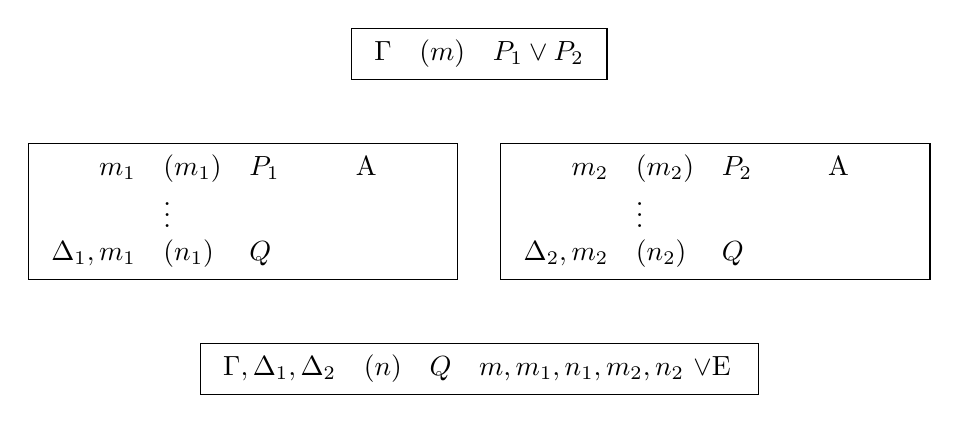
\begin{tikzpicture}  
  \node at (3,2)  (A) [draw,rectangle]{$ \begin{array}{l l l p{1cm}}
                                           \Gamma  & (m) & P_1\vee
                                                    P_2 \end{array}
                                                  $}; 
\node at (0,0) (B) [draw,rectangle]{%
  $ \begin{array}{r l >{$}p{1cm}<{$} p{1cm}}
      m_1 & (m_1) & P_1 & A \\
          & \vdots & \\
      \Delta _1,m_1 & (n_1) & Q & \end{array}$ };
\node at (6,0) (C) [draw,rectangle]{%
  $ \begin{array}{r l >{$}p{1cm}<{$} p{1cm}}
      m_2 & (m_2) & P_2 & A \\
          & \vdots & \\
      \Delta _2,m_2 & (n_2) & Q & \end{array}$ };
\node at (3,-2) (D) [draw,rectangle]{%
  $ \begin{array}{r l l p{3.25cm}}
       \Gamma ,\Delta _1,\Delta _2 & (n) & Q & $m,m_1,n_1,m_2,n_2$
                                               $\vee$E \end{array} $ % 
};
\end{tikzpicture}                                               
\caption{Disjunction elimination allows you to derive a conclusion
  from a disjunction by using two sub-arguments, one based on each disjunct.}
                                  \label{dilemma}
\end{figure}
Here we've used $\Gamma$ to represent the original background
information from which you derived the disjunction $P_1\vee P_2$.
When the $\vee$ elimination rule is invoked on line $n$, we have to
acknowledge dependency not only on $\Gamma$, but also on the
information in $\Delta _1$ and $\Delta _2$ that might have been used
in the two sub-arguments.

The reason we might need to bring other information into the
subarguments is so that we can use disjunctions together with other
premises in order to derive conclusions.  For example, consider the
premises $P\vee Q$ and $Q\to P$.  Obviously, these two premises
together should imply $P$.  Just consider the two cases: if $P$ then
of course $P$.  In the case of $Q$, we also have $Q\to P$, and hence
$P$.  But in making the second move here, we cannot forget the source
of our knowledge of $Q\to P$.  In other words, that premise needs to
be cited as well.  In official, regimented format, the argument would
go like this:
\[ \begin{array}{l l >{$}p{3cm}<{$} p{2cm}}
    1 & (1) & P\vee Q & A \\
    2 & (2) & Q\to P  & A \\
    3 & (3) & P       & A \\
    4 & (4) & Q       & A \\
    2,4 & (5) & P     & 2,4 MP \\
    1,2 & (6) & P & 1,3,3,4,5
    $\vee$E \end{array} \] The only mystery here is the exact recipe
used to calculate the dependencies of line 6.  Of course, line 6
should depend on whatever the disjunction on line 1 depends upon.  In
this case, line 1 depends only on itself.  Then we need to look at the
two sub-arguments.  The first sub-argument is completely trivial: it
starts with the assumption of $P$ on line 3, and it ends there.  It
simply infers $P$ from itself.  The second sub-argument starts with
the assumption of $Q$ on line 4; but then it uses line 2 to get line
5.  Thus, the second sub-argument presupposes line 2, and hence
whatever line 2 depends upon.  That's why we need to include line 2 in
the dependencies of line 6.  But we do {\it not} need to include lines
3 or 4 in the dependencies of line 6, because those were purely
hypothetical posits, used to see what follows from the disjunction
$P\vee Q$.  When we use disjunction elimination, we ``forget'' that
those subproofs ever happened, including the assumptions with which
they began.  We only remember the fact that both subproofs led to the
same conclusion.

We still need to tell you the {\it exact} recipe for calculating the
dependencies for a line that is justified by disjunction elimination.
We'll do that twice over, first giving a schematic proof.
\[ \begin{array}{r l >{$}p{2cm}<{$} p{3.5cm}}
    \Gamma    & (m)         & P_1\vee P_2 & \\
    m_1       & (m_1)       & P_1         & A \\
    &  \vdots     & \\
    \Delta _1,m_1    & (n_1) & Q   & \\
    m_2       & (m_2) & P_2 & A  \\
    & \vdots \\
    \Delta _2,m_2  & (n_2) & Q     \\
    \Gamma ,\Delta _1,\Delta _2 & (n) & Q &
    $m,m_1,n_1,m_2,n_2$ $\vee$E \end{array} \] That is, $\vee$E cites
five lines: a disjunction (line $m$), the assumption that begins the
first sub-argument (line $m_1$), the conclusion of the first
sub-argument (line $n_1$), the assumption that begins the second
sub-argument (line $m_2$), and the conclusion of the second
sub-argument (line $n_2$).  The dependencies of line $n$ are to be the
union of the following three collections of dependencies:
\begin{enumerate}
\item The dependencies $\Gamma$ of the disjunction $P_1\vee P_2$ on
  line $m$.
\item The dependencies $\Delta _1$ of the conclusion $Q$ on line
  $n_1$, except take away $m_1$ if it happens to occur among them.
\item The dependencies $\Delta _2$ of the conclusion $Q$ on line
  $n_2$, except take away $m_2$ if it happens to occur among them.
\end{enumerate}
In most applications, you'll follow this complicated recipe
subconsciously.  However, for those of you budding logicians who long
for full rigor, the precise set-theoretic calculation of the
dependencies on line $n$ is:
\[ \Gamma \cup (\Delta _1\backslash \{ m_1\})\cup (\Delta _2\backslash
  \{ m_2\}) ,\] which is just a symbolic representation of the words
we said previously.

As we've said before, we recommend that you try to understand abstract
rules by working on specific examples.  Let's start then with a proof
that $P$ follows from the disjunction $P\vee (P\wedge Q)$.
\[ \begin{array}{l l l p{2cm}}
    1 & (1) & P\vee (P\wedge Q) & A \\
    2 & (2) & P          & A \\
    3 & (3) & P\wedge Q  & A \\
    3 & (4) & P          & 3 $\wedge$E \\
    1 & (5) & P & 1,2,2,3,4
    $\vee$E \end{array} \] Here the first disjunct $P$ is assumed on
line $2$.  Of course, it immediately follows from the assumption of
$P$ --- without drawing any further inferences --- that $P$.  For this
reason, the application of $\vee$E on line 5 cites line 2 twice: once
as an assumption of the first disjunct, and once as the conclusion
drawn from the first disjunct.  The second disjunct $P\wedge Q$ is
assumed on line 3, and the conclusion $P$ is drawn again on line 4.
Thus, the application of $\vee$E on line 5 cites lines 3 and 4.
(Exercise: Suppose that you obtained line 5 from lines 1,2,2,3,2
instead of lines 1,2,2,3,4.  What then would be the dependencies of
line 5?)

We can now give a compact schematic statement of the disjunction
elimination rule.
\bigskip \begin{tcolorbox}[enhanced,width=7cm,title=disjunction
  elimination ($\vee$E),attach boxed title to top
  left={yshift=-2mm,xshift=4mm},boxed title style={sharp corners}]
  $ \begin{array}{c c c} \Gamma\:\vdash\: \phi \vee \psi \qquad
    \Delta ,\phi\:\vdash\:\chi \qquad \Theta ,\psi\:\vdash\:\chi \\
    \hline \Gamma ,\Delta ,\Theta\:\vdash\:\chi \end{array} $
\end{tcolorbox}
\bigskip \noindent So, the $\vee$E rule says that three separate
proofs can be converted into one proof.  Of course, you're not likely
to find those three proofs lying around; you'll usually have to make
them yourself. 

For example, suppose that you want to show $P\vee Q\vdash Q\vee P$.
Then you'd want to argue that the conclusion follows from each
disjunct separately, as follows.\marginnote{commutation \\
  $P\vee Q\:\vdash\:Q\vee P$}
\[ \begin{array}{l l >{$}p{2.5cm}<{$} p{2cm}}
    1 & (1) & P\vee Q & A \\
    2 & (2) & P       & A \\
    2 & (3) & Q\vee P & 2 $\vee$I \\
    4 & (4) & Q       & A \\
    4 & (5) & Q\vee P & 4 $\vee$I \\
    1 & (6) & Q\vee P & 1,2,3,4,5
    $\vee$E \end{array} \] In this case, the disjunction $P\vee Q$ is
an assumption, i.e.\ it hasn't been derived from something else.
Thus, the first input to $\vee$E on line 6 is the proof
$P\vee Q\vdash P\vee Q$.  The second input to $\vee$E on line 6 is the
sequent on line 3, namely $P\vdash Q\vee P$.  The third input to
$\vee$E on line 6 is the sequent on line 5, namely $Q\vdash Q\vee P$.
In this case then, $\vee$E permits us to write $Q\vee P$ on line 6,
with the following dependencies: (a) The dependencies $\Delta$ of the
disjunction $P\vee Q$ on line 1.  In this case, $\Delta$ is simply
$P\vee Q$ itself.  (b) The auxiliary assumptions $\Gamma$ that may
have been used to derive $Q\vee P$ from the first disjunct $P$.  In
this case, $\Gamma$ is empty.  (c) The auxiliary assumptions $\Delta$
that may have been used to derive $Q\vee P$ from the second disjunct
$Q$.  In this case, $\Delta$ is empty.

For an even simpler --- and yet possibly more confusing ---
application of $\vee$E, we derive $P$ from the disjunction $P\vee P$.
\[ \begin{array}{l l >{$}p{2cm}<{$} p{2.5cm}}
    1 & (1) & P\vee P & A \\
    2 & (2) & P       & A \\
    1 & (3) & P & 1,2,2,2,2
    $\vee$E \end{array} \] Here the first and second disjuncts are the
same sentence, namely $P$.  Hence, the assumption on line 2 can serve
as the assumption for both sub-proofs.  In addition, the desired
conclusion is simply $P$ again, hence line 2 can serve as the
conclusion of both sub-proofs.  It's for this reason that the
invocation of $\vee$E on line 3 cites line 2 four times: twice as an
assumption, and twice as the conclusion of sub-proofs.

It might also help to see an example where the disjunction elimination
rule has been {\it misapplied}.  Intuitively, it shouldn't be possible
to prove $P$ from $P\vee Q$.  For example, from the fact that the
number $2$ is either even or odd, you shouldn't be able to deduce that
it's odd!  But consider the following attempt to prove $P$ from
$P\vee Q$.
\[ \begin{array}{l l >{$}p{2cm}<{$} p{2cm} p{3cm}}
     1 & (1) & P\vee Q & A \\
     2 & (2) & P       & A \\
     3 & (3) & Q       & A \\
     2,3 & (4) & P\wedge Q & 2,3 $\wedge$I \\
     2,3 & (5) & P         & 4 $\wedge$E \\
     1   & (6) & P         & 1,2,2,3,5 $\vee$E & $\Longleftarrow$ incorrect \end{array} \]
Everything in this ``proof'' is OK except for the dependencies of line
6.  The problem is that line 6 should include all the dependencies of
line 5 (i.e.\ the conclusion of the second sub-proof) except for 3
(i.e.\ the assumption of that sub-proof).  Thus, line 6 should also
include 2 among its dependencies.  But in that case, it would be a
proof of $P\vee Q,P\vdash P$, which is not so surprising after all.

\begin{exercises} Prove the following sequents.
  \begin{enumerate}
  \item $(P\to R)\wedge (Q\to R)\:\vdash\: (P\vee Q)\to R$  
  \item association: $P\vee (Q\vee R)\:\dashv\vdash\: (P\vee Q)\vee R$
  \item disjunctive syllogism: $P\vee Q,\neg P\:\vdash \: Q$
%% Hint: use P,\neg P\vdash Q on the LHS
\item distribution: $P\wedge (Q\vee R)\:\dashv\vdash\: (P\wedge Q)\vee (P\wedge R)$
\item distribution: $P\vee (Q\wedge R)\:\dashv\vdash\: (P\vee Q)\wedge (P\vee R)$
\item material conditional: $\neg P\vee Q\:\dashv\vdash\: P\to Q$
\item \gls{dm}: $\neg P\vee \neg Q\:\vdash\: \neg (P\wedge Q)$  
  \end{enumerate}
\end{exercises}

In the previous exercises, you proved that $P\vee (Q\vee R)$ is
equivalent to $(P\vee Q)\vee R$.  Accordingly, in some later
discussions, we might allow ourselves to write $P\vee Q\vee R$, when
we don't need to specify which of the equivalent sentences we're
talking about.

\section{Reductio ad Absurdum}

We began the book by stating that logic is a tool to sort between true
and false claims.  To this point, it might seem that the primary role
of logic is to establish which claims are true, by showing that they
are logical consequences of claims that we already know to be true.
However, logic may be even more effective when applied in reverse: to
show which claims cannot possibly be true.

Imagine, for example, that your friend Angelina has a certain belief
$P$ which you are quite sure is false.  Suppose also that Angelina,
like you, is quite good at logic, and she knows the difference between
good and bad arguments.  Here then is a very effective way to convince
Angelina to reject $P$: give her a valid proof that begins with $P$
(and possibly some other agreed upon background information $\Gamma$)
and that ends with some conclusion $C$ that Angelina rejects.  Since
we're supposing that Angelina is completely logical, she'll be forced
then either to give up $P$, or to change her mind about $C$.

Now, in the most extreme case, $C$ could be something that not only
Angelina, but every rational person, must reject.  In particular, $C$
might be a logical contradiction such as $\psi\wedge\neg \psi$.  We'll
take this extreme case to be paradigmatic of an argumentative strategy
called \gls{raa}, which literally means ``reducing to absurdity.''
The idea, again, is that if a statement $\phi$ leads to an absurdity
$\psi\wedge\neg \psi$, then $\phi$ must be rejected.  This
argumentative strategy can be formalized as follows:

\bigskip 
\begin{tcolorbox}[enhanced,width=10cm,title=reductio ad absurdum (RAA),attach boxed title to top
  left={yshift=-2mm,xshift=4mm},boxed title style={sharp corners}]
  A proof of \mbox{$\psi\wedge\neg \psi$} from $\Gamma$ and $\phi$ can
  be converted to a proof of $\neg \phi$ from $\Gamma$.
  Schematically:
  $\begin{array}{r@{\:\,}c@{\:\,}l} \Gamma ,\phi &\vdash & \psi\wedge
    \neg \psi \\ \hline \Gamma &\vdash & \neg \phi \end{array} $
 \end{tcolorbox} \bigskip

 When written in linear format, RAA must cite two lines: (1) an
 assumption, say of $\phi$, and (2) a contradiction, such as
 $\psi\wedge\neg \psi$.  The conclusion of RAA then depends on
 whatever the contradiction $\psi\wedge\neg \psi$ depends upon, except
 possibly the assumption of $\phi$.\footnote{As with conditional
   proof, the contradiction is not required to depend on the
   assumption of $P$.}

The following is a fairly standard use of RAA.
\[ \begin{array}{l l >{$}p{2cm}<{$} p{1.5cm}}
     1 & (1) & P\to Q & A \\
     2 & (2) & P\to \neg Q & A \\
     3 & (3) & P & A \\
     1,3 & (4) & Q & 1,3 MP \\
     2,3 & (5) & \neg Q & 2,3 MP \\
     1,2,3 & (6) & Q\wedge \neg Q & 4,5 $\wedge$I \\
     1,2 & (7) & \neg P & 3,6 RAA \end{array} \] %
 Here the assumption of $P$ is used to detach $Q$ and $\neg Q$ from
 the conditionals in lines 1 and 2.  It is, however, acceptable to
 apply RAA even if the assumption is not used --- as in the following
 alternative proof of \gls{efq}. %
 \[ \begin{array}{l l >{$}p{2cm}<{$} p{1.5cm}}
      1 & (1) & Q\wedge \neg Q & A \\
      2 & (2) & \neg P & A \\
      1 & (3) & \neg \neg P & 2,1 RAA \\
      1 & (4) & P & 3 DN \end{array} \] %
Here the assumption (line 2) comes after the contradiction (line 1).  That might feel like
cheating --- in the same way that it feels like cheating to use
conditional proof in a case where the assumption of the antecedent
comes after the derivation of the consequent.  However, the RAA rule
permits this move.  Note also that since the assumption (line 2)
wasn't used to derive the contradiction (line 1), the dependencies on
line 3 are the same as those on line 1.

%% RAA is eliminable, which means that EM could already have been proven

As in the previous argument, RAA is frequently used in combination
with DN, and this combination makes RAA a powerful tool for proving
positive results.  In general, to establish a positive result $P$, all
you need to do is to show that its negation $\neg P$ leads to a
contradiction.  This combination (RAA and DN) can be used to give
another proof of \gls{em}. 
\[ \begin{array}{l l >{$}p{5cm}<{$} p{2cm} l l}
     1 & (1) & \neg (P\vee \neg P) & A \\
     2 & (2) & P & A \\
     2 & (3) & P\vee \neg P & $2$ $\vee$I \\
     1,2 & (4) & (P\vee \neg P)\wedge \neg (P\vee \neg P) & $3,1$ $\wedge$I  \\
     1 & (5) & \neg P & $2,4$ RAA \\
     1 & (6) & P\vee \neg P & $5$ $\vee$I \\
     1 & (7) & (P\vee \neg P)\wedge \neg (P\vee \neg P) & $6,1$ $\wedge$I \\
       & (8) & \neg \neg (P\vee \neg P) & $1,7$ RAA \\
       & (9) & P\vee \neg P &
                              $8$ DN \end{array} \] \gls{em} can be a
 useful auxiliary for proving other things.  In fact, \gls{em} and \gls{raa} are the tools of choice for proving things that have eluded all other methods of attack.  Consider, for example, the following valid sequent:
 \[ \vdash\:((P\to Q)\to P)\to P \] It's not at all obvious how one
 could prove this sequent.  Since it's a conditional sentence, you
 might try to assume the antecedent $(P\to Q)\to P$, and then to
 derive the consequent $P$.  However, since the antecedent is a
 conditional sentence, there is nothing that you can infer from it, at
 least until you assume something else.  If you go on like this for a
 while, you might find yourself increasingly flustered.  Let's then
 bring out the big guns: first write down a proof of $P\vee \neg P$.
 Now set up two sub-proofs, one beginning with the assumption of $P$
 and the other with the assumption of $\neg P$.  The first sub-proof
 immediately yields the consequent that you want, namely $P$.  For the
 second sub-proof, recall negative paradox: $\neg P\vdash P\to Q$.
 Hence from $\neg P$, you could derive $P\to Q$, and then in
 combination with the assumption $(P\to Q)\to P$, you could derive
 $P$.  The overall structure of this derivation looks like this:
\[ \begin{array}{>{$}p{1.2cm}<{$} >{$}p{4.5cm}<{$} p{3cm}}
     & \vdots  \\
     & P\vee \neg P & \gls{em} \\
     \ast  & P            & A \\
     \star & \neg P       & A \\
     & \vdots       &   \\
     \star   & P\to Q       & negative paradox \\
     \dagger  & (P\to Q)\to P & A \\
     \star ,\dagger   & P   \\
     \dagger   & P     & $\vee$E \\
     & ((P\to Q)\to P)\to P & CP \end{array} \] %
Here the symbols $\ast ,\star ,\dagger$ stand in for unknown
dependency numbers.  Of course, if you filled in all the steps, this
proof would be quite long.  In the next section, we will explain a
method for citing one proof inside another so that you can keep your
proofs to a manageable length.

\begin{exercises} Prove the following sequents.
\begin{enumerate}
\item material conditional: $P\to Q\:\vdash\: \neg (P\wedge \neg Q)$  
\item \gls{dm}: $\neg (P\wedge Q)\:\vdash\: \neg P\vee \neg Q$
\item material conditional: $\neg (P\to Q)\:\vdash\: P\wedge \neg Q$     
\sitem chain order: $\vdash (P\to Q)\vee (Q\to P)$
     % (Hint: Prove $P\vee \neg P$, then use positive and negative
     % paradox.)
\sitem $P\to (Q\vee R)\:\vdash\: (P\to Q)\vee (P\to R)$
\item $(P\wedge Q)\to \neg Q\:\vdash\:P\to \neg Q$
\end{enumerate}  

\begin{exercise} People who reject DN elimination also tend to reject
  the law of excluded middle.  This exercise explains why.  Use the
  law of excluded middle and EFQ to re-derive DN elimination.  That
  is, show that $\neg\neg P\vdash P$, without using DN, but where
  you're allowed to insert $P\vee\neg P$, and where you're allowed to
  infer anything from a contradiction.

  For discussion: is the law of excluded middle more obviously correct
  than the DN rule?
\end{exercise}

  %% TO DO: need to introduce biconditional  

%% TO DO: classical logic has the funny property that $\vdash A\vee B$
%% doesn't entail that either $\vdash A$ or $\vdash B$.  

\end{exercises}


%%% Local Variables:
%%% mode: latex
%%% TeX-master: "main"
%%% End:


\chapter{New Proofs from Old} \label{new}

As the old saying goes, ``don't work harder, work smarter.''  You've
done the hard work writing a lot of proofs; now it's time to work
smarter.  In this chapter, we're going to think about how you can
reliably take short-cuts with proofs.  The key word here is
``reliably.''  That is, we want to ensure that these shortcuts won't
cause you to misjudge whether or not something can be proven.

For example, suppose that we ask you to prove the sequent:
$\vdash (P\to Q)\vee \neg (P\to Q)$. You've probably never proved this
sequent before.  However, you should have -- if you've been diligent
-- proved an instance of the law of excluded middle, i.e.\ something
like $\vdash P\vee \neg P$.  Now suppose that you have the proof of
$P\vee\neg P$ saved in a file \texttt{em.txt}, and that you run a
``find and replace'' to swap in $P\to Q$ for $P$.  Then, the result
will be a proof of $(P\to Q)\vee \neg (P\to Q)$.  That's working
smart: take an old proof, run find-and-replace, and ta da, you have a
new proof.

What we just did was a case of {\it substitution}.  We'll discuss
substitution in the first section.  Then we'll talk about another
short-cut method that allows you to splice an old proof into a new one
--- the method of {\it cut}.  Finally, we'll talk about a third
short-cut method that allows you to {\it replace} a sub-formula with
any logically equivalent sub-formula.  If you learn these three
methods, you'll be able to prove even the most challenging
propositional logic sequents with ease.


\section{Substitution}

In this section, we describe the theoretical basis for the
``find-and-replace'' method of generating new proofs from old.  To
this end, we first need to define the notion of a
\emph{\gls{substitution instance}}. \index{substitution instance} The
idea here is that the find-and-replace operation changes a formula
$\phi$ to a substitution instance $\phi ^*$, and a proof of
$\phi\vdash\psi$ to a proof of $\phi ^*\vdash\psi ^*$.

Each sentence of our symbolic language is either one of the symbols
$P,Q,R,\dots $, or it's built up from those symbols using the
connectives $\neg,\wedge ,\vee$ and $\to$.  It's time to be a bit more
precise about the ways in which we permit sentences to be constructed.
We call the capital letters $P,Q,R\dots $ our \emph{\glspl{atomic
    sentence}}, the idea being that they have no internal structure.
\index{sentence!atomic} We also stipulate that if $\phi$ and $\psi$
are sentences, then $\neg\phi$, $\phi\wedge\psi$, $\phi\vee\psi$, and
$\phi\to\psi$ are also sentences.  (To be even more precise, we have
to put parentheses around the resulting sentence at each stage of
construction.  However, we will omit parentheses after applying
$\neg$, and we will omit the outermost parentheses from every
sentence.)  What's more, we stipulate that all legitimate sentences
come about from applying a finite number of these construction steps.

We now define a notion of a
\emph{\gls{translation}}. \index{translation} For simplicity, let's
suppose that we begin with a list $P,Q,R,\dots $ of simple sentences.
A \emph{\gls{reconstrual}} \index{reconstrual} is an assignment $F$ of
each atomic sentence $X$ to some other sentence $F(X)$.  For example,
$F(P)$ could be another atomic sentence, such as $R$, or it could be a
complex sentence such as $R\to \neg S$, or even $\neg P$ or
$P\wedge\neg P$.  There are no restrictions at all on the assignment
$F$, so long as the result is a legitimate sentence.

Once we have a reconstrual $F$, we can use it to translate {\it any}
sentence $\phi$.  In short, we define $F(\phi )$ to be the sentence
that results from replacing each atomic sentence $X$ in $\phi$ with
$F(X)$.  The resulting string of symbols $F(\phi )$ will always be a
legitimate sentence, and we call it a substitution instance of $\phi$.

As usual, the definition becomes more clear when we look at examples.
Suppose, for example, that we reconstrue $P$ as $Q\to P$, and $Q$ as
$\neg R$.  That reconstrual results in the following substitution instances.
\[ \begin{array}{l l l}
     P\to Q & \leadsto  & (Q\to P)\to \neg R \\
     P\vee \neg P & \leadsto  & (Q\to P)\vee \neg (Q\to P) \\
     Q\to P & \leadsto & \neg R \to (Q\to P) \end{array} \] It should
be clear that there is some sense in which the substitution operation
preserves the form of the original sentence; or, to be more precise,
that $F(\phi )$ is an instance of the form presented by $\phi$.
However, $F(\phi )$ can have more structure than $\phi$ itself has;
for example, {\it every} sentence is a substitution instance of the
atomic sentence $P$.

%% exercise

\begin{exercise} Which of the following formulas is a substitution instance of
  the formula $P\to \neg Q$?  In cases where you answer affirmatively,
  show how to reconstrue $P$ and $Q$ to get the resulting formula.
\begin{enumerate}
\item $\neg Q\to \neg P$
\item $(P\to \neg Q)\to R$
\item $(P\to \neg Q)\to \neg (P\to \neg Q)$.
\end{enumerate}  
\end{exercise}

Recall that our inference rules are schematic, i.e.\ they depend only
on the form of the sentences involved.  Thus, it should immediately
follow that substitution preserves validity, since it preserves form.
We will prove that rigorously in Chapter \ref{meta}, with a result
known as the \emph{substitution theorem}.  But for now, it will
suffice to state the upshot, which we can use to generate new proofs
from old ones.

\bigskip 
\begin{tcolorbox}[enhanced,width=10cm,title=substitution,attach boxed title to top
  left={yshift=-2mm,xshift=4mm},boxed title style={sharp corners}]
  A proof of $\phi _1,\dots ,\phi _n\vdash\psi$ can be converted to a
  proof of $F(\phi _1),\dots ,F(\phi _n)\vdash F(\psi )$, where $F$ is
  a reconstrual of the non-logical vocabulary.
\end{tcolorbox}
\bigskip

The \emph{substitution meta-rule} is just a formalization of what you
already know: that find-and-replace preserves the validity of proofs
(as long as you restrict the finding to atomic sentences, and you
replace them with other well-formed sentences).  Note that
substitution is not a rule in the same sense as, say, modus ponens,
which generates new valid inferences.  To illustrate this point,
imagine that proofs of all valid sequents are saved in some computer
file $\mathsf{proofs.txt}$.  Each such proof consists of finitely many
lines, and in the right hand column, every line is justified by one of
the inference rules: $\wedge I$, $\wedge E$, MP, etc.  None of those
lines is justified by some rule called ``substitution.''  Instead, the
substitution meta-rule tells us that for any proof in
$\mathsf{proofs.txt}$, there is another proof in $\mathsf{proofs.txt}$
that looks just like the first, except that the atomic sentences have
been replaced by some other sentences.

\begin{exercise} Do you think the following claims are true or false?
  Explain your answers.
  \begin{enumerate}
  \item If $\phi$ is not provable, then no substitution instance of
    $\phi$ is provable.
  \item The sentence $(P\wedge Q)\to R$ has a substitution instance
    that can be proven.
    %% For each sentence $\psi$, if $\psi$ doesn't imply $\bot$, then
    %% there is an elementary conjunction $\phi$ such that
    %% $\phi\vdash\psi$.
  \end{enumerate} \end{exercise}

\section{Cut}

We now introduce a key meta-rule that, if used correctly, can greatly
increase your efficiency in proving things.  Let's begin with an
example.

Suppose that you've been asked to prove that
\[ P\to (Q\vee R)\:\vdash\: (P\to Q)\vee (P\to R) .\] After many
failed attempts, you might decide to bring out the sledgehammer of
reductio ad absurdum: to assume the negation of the result you want,
and derive a contradiction.  Now, the negation
$\neg ((P\to Q)\vee (P\to R))$ doesn't look to be all that useful.
However, you might then remember that you've already proven the
following version of DeMorgan's rule:
$\neg (P\vee Q)\vdash \neg P\wedge \neg Q$.  You could then substitute
$P\to Q$ for $P$, and $P\to R$ for $Q$, which gives you a proof of
\[ \neg ((P\to Q)\vee (P\to R)) \: \vdash \: \neg (P\to Q)\wedge \neg
  (P\to R) .\] But now you've got to figure out how to splice that
proof into the proof you're currently working on.  The cut meta-rule
will allow you to perform this splice, yielding the following lines:
\[ \begin{array}{l l >{$}p{4.5cm}<{$} p{3cm}}
     1 & (1) & P\to (Q\vee R) & A \\
     2 & (2) & \neg ((P\to Q)\vee (P\to R)) & A \\
     2 & (3) & \neg (P\to Q)\wedge \neg (P\to R) & cut,
                                                   DM \end{array} \]
The basic idea here is that if you've proven a sequent
$\phi\vdash\psi$ (such as DeMorgan's), then you can use that sequent
to continue a proof from a line with $\Gamma\vdash\phi$ to a line with
$\Gamma\vdash\psi$.  We state the rule, however, in a more general fashion.

\bigskip \begin{tcolorbox}[enhanced,width=10cm,title=cut,attach boxed
  title to top left={yshift=-2mm,xshift=4mm},boxed title style={sharp
    corners}]
  Suppose that you have already demonstrated that \newline
  $\phi _1,\dots ,\phi _n\vdash\psi$.  Then in any proof where you
  have lines $\Gamma _1\vdash\phi _1,\dots ,\Gamma _n\vdash\phi _n$,
  you may infer that $\Gamma _1,\dots ,\Gamma _n\vdash \psi$.
\end{tcolorbox}
%% justification
\bigskip As with substitution, cut is not a new inference a new rule.
Instead, it's a promise: if certain proofs exist, then so does another
proof.  Imagine again a computer file $\mathsf{proofs.txt}$ that
contains all correctly written proofs.  The word ``cut'' does not
appear in any of those proofs.  However, if $\mathsf{proofs.txt}$
contains proofs of $\phi _1,\dots ,\phi _n\vdash\psi$, and also of
each $\Gamma _i\vdash\phi _i$, then cut promises that
$\mathsf{proofs.txt}$ also has a proof of
$\Gamma _1,\dots ,\Gamma _n\vdash\psi$.  That latter proof, however,
only cites the primitive inference rules such as $\wedge I$ and $MP$.

When you write proofs, however, you can cite cut, because you're
giving your reader a promise that you could expand it out into a
correctly written proof.  For example, suppose that you already have a
proof of the sequent $\phi\vdash\psi$ (which you named ``hocus
pocus''), and that you've begun a new proof where $\phi$ appears on
line $m$.  Then on a subsequent line, you can write $\psi$ with a
citation of cut.
\[ \begin{array}{l l l p{3cm}}
     \Gamma & (m) & \phi & \\
            & \vdots \\
     \Gamma & (n) & \psi & cut, hocus pocus \end{array} \] If somebody
 then calls you on the cut, you can do the following: take the proof of $\phi\vdash\psi$ and add a line of CP to get a proof of $\vdash\phi\to\psi$.  Then instead of citing cut on line $n$, copy in that entire proof, and finish with a step of MP.
\[ \begin{array}{l l >{$}p{1.75cm}<{$} p{2cm}}
     \Gamma & (m) & \phi & \\
            & \vdots \\
            & (n_1) & \phi\to\psi  & \\
     \Gamma & (n_2) & \psi         & $m,n_1$ MPP \end{array} \]
So, using cut with an already proven sequent is just a way of
indicating that you could write a proof.  

Many cases of cut involve the special case $n=1$, i.e.\ where you've
already demonstrated that $\phi\vdash\psi$, and you find yourself with
a line like this:
\[ \begin{array}{l l l p{3cm}}
     \Gamma & (m) & \phi  & \end{array} \]
In this case, cut licenses the following inference:
 \[ \begin{array}{l l >{$}p{1cm}<{$} p{3cm}}
      \Gamma & (n) & \psi & $m$ cut \end{array} \]
For an example of cut with $n=2$, suppose that you have proved
disjunctive syllogism $P\vee Q,\neg P\vdash Q$, and that you have the
following two lines in a proof:
\[ \begin{array}{r l l p{3cm}}
     \Gamma _1 & (m) & P\vee Q \\
     \Gamma _2 & (n) & \neg P  \end{array} \]
 Then cut licenses a subsequent line:
 \[ \begin{array}{r l >{$}p{1cm}<{$} p{3cm}}
      \Gamma _1,\Gamma _2 & (n') & Q & $m,n$ cut \end{array} \]

  The cut rule is also really useful in the case where $n=0$.  In that
  case, we have already proven a single sequent $\vdash\psi$ that has
  no premises.  The cut rule then says that on any line of a
  subsequent proof, we may write $\psi$ with no dependencies.  So, for
  example, if we've already proven the law of excluded middle (lem),
  $P\vee\neg P$, then any time we're writing a proof, we may insert a
  line:
 \[ \begin{array}{l c >{$}p{1.5cm}<{$} p{4cm}}
  & (n) & P\vee\neg P & cut, LEM \end{array} \]
%% don't forget to extend to SI(s)
This invocation of cut goes beyond substitution, because substitution
only creates an entire new proof.  Cut allows you to paste an old
proof in the middle of a new one.

You can, however, use cut together with substitution.  For example, if
you've proven excluded middle, then substitution gives you a proof of
$\vdash (P\to Q)\vee \neg (P\to Q)$.  Then cut permits you to drop
this sequent into a proof as follows:
 \[ \begin{array}{l c >{$}p{4cm}<{$} p{4cm}}
  & (n) & (P\to Q)\vee\neg (P\to Q) & cut, LEM \end{array} \]
Technically speaking, this line $n$ should say something like
``substitution + cut''.  But substitution is so immediate that it can
typically be used without mention.

Let's look at one more example of the use of cut.  We'll take for
granted that you already have proofs of excluded middle
$\vdash P\vee \neg P$, and positive paradox $P\vdash Q\to P$.  We will
use these results to prove the sequent $\vdash (P\to Q)\vee (Q\to P)$.
\[ \begin{array}{l l >{$}p{4cm}<{$} p{4cm}}\
       & (1) & P\vee \neg P  &   cut, lem \\
     2 & (2) & P             &   A \\
     2 & (3) & Q\to P        &   2 cut, pos paradox \\
     2 & (4) & (P\to Q)\vee (Q\to P) & 3 $\vee$I \\
     5 & (5) & \neg P        &   A \\
     5 & (6) & \neg Q\to \neg P & 5 cut, pos paradox \\
     2 & (7) & \neg \neg P   & 2 DN \\
     2,5 & (8) & \neg\neg Q   & 6,7 MTT \\
     2,5 & (9) & Q            & 8 DN \\
     5   & (10) & P\to Q       & 2,9 CP \\
     5   & (11) & (P\to Q)\vee (Q\to P) & 10 $\vee$I \\
         & (12) & (P\to Q)\vee (Q\to P) & 1,2,4,5,11 $\vee$E                                
   \end{array} \]
 On line 2 we have the sequent $P\vdash P$.  Positive paradox establishes
 the sequent $P\vdash Q\to P$.  Hence, cut permits us to combine these
 two sequents into $P\vdash Q\to P$, which we write on line 3.  
 We then use positive paradox again to obtain line 6 from line 5.
 (Note that if we had permitted ourselves to use negative paradox, then
 we could immediately have obtained $P\to Q$ from line 5.)

%% TO DO: powerful to combine substitution with cut

\section{If and Only If}

We have one more meta-rule to cover, viz.\ the replacement rule.
However, we pause to define a symbol that will facilitate our
discussion of replacement.

If you spend any amount of time hanging around mathematicians or
analytic philosophers, you'll pick up the phrase ``if and only if.''
This phrase is meant to express something even stronger than a
conditional; it's meant to express a two-directional conditional, or
\emph{\gls{biconditional}}.  For example, if I tell you that
\begin{quote} You will get an A on the exam if and only if you
  study \end{quote} then I'm telling you two things.  First, ``you
will get an A on the exam if you study,'' which means that studying is
a \emph{sufficient condition} for getting an A on the exam.  Second,
``you will get an A on the exam only if you study,'' which means that
studying is a \emph{necessary condition} for getting an A on the exam.

We will use the symbol $\lra$ for the ``if and only if'' connective.
Like a conditional, this connective applies to two sentences; thus, if
$\phi$ and $\psi$ are sentences of propositional logic, then so is
$\phi\lra\psi$.  In order for this new connective to be useful, we now
have to specify its inference rules.  Fortunately, its meaning is
completely transparent, once we already know how to express ``if \dots
then \dots '', and ``and''.  In particular, $\phi\lra\psi$ should be
equivalent to $(\phi\to\psi )\wedge (\psi\to\phi )$.  In fact, we will
make this equivalence into a definition of the introduction and
elimination rules.


\bigskip 
\begin{tcolorbox}[enhanced,width=11cm,title=biconditional introduction
  ($\lra$I) and elimination ($\lra$E),attach boxed title to top
  left={yshift=-2mm,xshift=4mm},boxed title style={sharp corners}]
\[ \begin{array}{c c c}  \begin{array}{c c} \Gamma\:\vdash\: (\phi\to \psi)\wedge (\psi\to \phi) \\
                              \hline \Gamma\:\vdash\: \phi\lra \psi \end{array} & &
                                                                                 \begin{array}{c c} \Gamma\:\vdash\: \phi\lra \psi \\ \hline
\Gamma\:\vdash\: (\phi\to \psi )\wedge (\psi\to \phi ) \end{array} \end{array} \]                                                                                   
\end{tcolorbox}
\bigskip 

To check that these are good inference rules, let's first verify that
``$P$ if and only if $P$'' is tautologous.
\[ \begin{array}{l l >{$}p{3.5cm}<{$} p{3cm}}
1 & (1) & P & A \\
  & (2) & P\to P & 1,1 CP \\
  & (3) & (P\to P)\wedge (P\to P) & 2,2 $\wedge$I \\
  & (4) & P\lra P  & 3 $\lra$I \end{array} \]
In technical writing, people often abbreviate ``if and only if'' to
the three letters ``iff''.  Another expression that is sometimes used 
with the same force is ``just in case''.  In particular,
mathematicians often state their definitions by saying something like,
``We'll say that a number $n$ is {\it prime} just in case \dots ''.
By this they mean, a number $n$ is prime if and only if \dots .

Recall that a conditional $P\to Q$ in propositional logic can be
asserted in conditions considerably weaker than those that license
asserting a conditional in some everyday life contexts.  In
particular, $Q\vdash P\to Q$, which means that $Q$ itself is a
sufficient condition for $P\to Q$.  This result also suggests that
$P\lra Q$ should be assertable in any context where both $P$ and $Q$
are assertable.  We verify that fact now.
\[ \begin{array}{l l >{$}p{4cm}<{$} p{4cm}}
      1 & (1) & P\wedge Q & A \\
      1 & (2) & Q & 1 $\wedge$E \\
      1 & (3) & P\to Q & 2 cut, positive paradox \\
      1 & (4) & P  & 1 $\wedge$E \\
      1 & (5) & Q\to P & 4 cut, positive paradox \\
      1 & (6) & (P\to Q)\wedge (Q\to P) & 3,5 $\wedge$I \\
      1 & (7) & P\lra Q   & 6 $\lra$I \end{array} \]
This proof yields the sequent $P\wedge Q\vdash P\lra Q$.  A similar
proof (see the exercises) shows that $\neg P\wedge\neg Q\vdash P\lra
Q$.  You could then combine these two proofs with a step of
disjunction elimination to prove the sequent:
\[ (P\wedge Q)\vee (\neg P\wedge\neg Q)\: \vdash \: P\lra Q .\]

\begin{exercises} Prove the following sequents.  You may invoke cut
  with any named sequent that you have already proven (e.g.\ lem,
  positive paradox, negative paradox).
   \begin{enumerate}
\item $P\lra Q\:\vdash\: Q\lra P$     
\item $\vdash\: (Q\to P)\vee (P\to R)$     
\item $P\lra Q\:\dashv\vdash\: (P\wedge Q)\vee (\neg P\wedge \neg Q)$     
\item $\neg (P\lra P)\:\vdash\: Q\wedge\neg Q$
\item $P\lra Q, Q\lra R\:\vdash\: P\lra R$
\item $\neg (P\lra Q)\:\dashv\vdash\: (P\lra \neg Q)$  
\item $\vdash\: (P\lra Q)\vee (P\lra R)\vee (Q\lra R)$
\end{enumerate}
\end{exercises}


%% TO DO: more complicated substitution -- i.e. replacement

\section{Replacement} \label{replacement}

The substitution meta-rule permits only transformations that begin
with atomic sentences, and that propagate through the application of
the logical connectives.  The \emph{replacement meta-rule} is more
flexible: it permits replacement of an entire subformula.

The idea behind this meta-rule is simple.  Suppose that you have
proven both sequents $\phi\vdash\psi$ and $\psi\vdash\phi$.  So, you
know then that $\phi$ and $\psi$ are equivalent, ``for all logical
purposes.''  In particular, whatever inferential relations $\phi$
stands in to any other sentence $\theta$, $\psi$ stands in exactly
those same inferential relations to $\theta$.  This suggests that in
any argument, $\psi$ should be able to play the same role as $\phi$.

For example, consider the sequent
\[ R\vee ((Q\to R)\to P) \: \vdash \: R\vee ((\neg Q\vee R)\to P) .\]
This sequent could be proven the long way around by performing
disjunction elimination.  After assuming the second disjunct of the
premise, you could then assume $\neg Q\vee R$.  Then plug in the proof
of $\neg Q\vee R\vdash Q\to R$, and so on.

Let $\theta$ be the formula $Q\to R$, let $\theta '$ be the formula
$\neg Q\vee R$, and let $\phi$ be the formula $R\vee ((Q\to R)\to P)$.
In other words, $\phi$ is the formula $R\vee (\theta \to P)$, and the
conclusion of the argument is the formula $R\vee (\theta '\to P)$.

After doing many proofs, you'll start to get the feeling that a move
like this can always be done.  That is, if one formula $\theta$ occurs
as part of another $\phi$, and if $\theta$ is provably equivalent to
$\theta '$, then you'll always be able to find a proof $\phi\vdash\phi
[\theta '/\theta ]$, where $\phi [\theta '/\theta ]$ is the formula
you get if you replace $\theta$ in $\phi$ with $\theta '$.

But can you be sure that it will always work?  The answer is yes, that
you can be sure, but it takes some patient verification to see why.
The key here is simply to check that all of the connectives preserve
inter-derivability of sentences.  So, for example, if $\theta$ and
$\theta '$ are inter-derivable, then no matter what sentence $\psi$
is, the conjunction $\theta\wedge\psi$ will be inter-derivable with
$\theta' \wedge\psi$, the conditional $\theta\to\psi$ will be
inter-derivable with $\theta'\to\psi$ and so on.  If we apply the same
thought again, it follows that $\chi\vee (\theta\wedge\psi )$ is
inter-derivable with $\chi\vee (\theta '\wedge\psi )$, and so on.  In
other words, once you have that $\theta\dashv\vdash\theta '$, then
$\theta$ can be embedded as deeply as you want in some other formula
$\phi$, and it will still be the case that $\phi\dashv\vdash \phi
[\theta '/\theta ]$, where $\phi [\theta '/\theta ]$ is the result of
replacing $\theta$ in $\phi$ with $\theta '$.

Our meta-rule of replacement can be made more convenient for proving
stuff if we remember that $\phi\dashv\vdash\phi [\theta /\theta ']$
implies that if $\Gamma\vdash\phi$ then
$\Gamma\vdash\phi [\theta /\theta ']$.  That is, if there's a proof of
$\phi$ from $\Gamma$, then there's also a proof of
$\phi [\theta /\theta ']$.

\bigskip \begin{tcolorbox}[enhanced,width=10cm,title=replacement with
  an equivalent (RE),attach boxed title to top
  left={yshift=-2mm,xshift=4mm},boxed title style={sharp corners}]
  Given a line \mbox{$\Gamma\vdash\phi$ of a proof}, and a sub-formula
  $\theta$ of $\phi$, if $\theta$ is equivalent to $\theta '$, then
  you may infer a sub{-}sequent line
  $\Gamma\vdash\phi [\theta '/\theta]$, where $\theta$ has been
  replaced by $\theta '$.  Schematically: \[ \begin{array}{c c}
       \vdash\theta\lra\theta ' \qquad \Gamma\vdash\phi \\ \hline
       \Gamma\vdash \phi [\theta '/\theta] \end{array} \]
\end{tcolorbox}

\bigskip The replacement meta-rule can be used with any equivalences
that have already been proven.  If you keep in mind some key
equivalences (see page \pageref{equivs}), then it can really speed up
proofs.  Consider, for example, the following alternative proof of
Peirce's law.
 % \[ \begin{array}{l l l p{4cm}}
 %      1 & (1) & (P\to Q)\to P  & A \\
 %      2 & (2) & \neg P         & A \\
 %      1,2 & (3) & \neg (P\to Q) & 1,2 MTT \\
 %      1,2 & (4) & P\wedge\neg Q & 3 mat cond \\
 %      1,2 & (5) & P             & 4 $\wedge$E \\
 %      1,2 & (6) & P\wedge \neg P & 5,2 $\wedge$I \\
 %      1   & (7) & \neg \neg P    & 2,6 RAA \\
 %      1   & (8) & P              & 7 DN \end{array} \]
\[ \begin{array}{l l >{$}p{3cm}<{$} p{4cm}}
     1 & (1) & (P\to Q)\to P  & A \\
     1 & (2) & \neg (P\to Q)\vee P & 1 RE, mat cond \\
     1 & (3) & (P\wedge \neg Q)\vee P & 2 RE, mat cond \\
     4 & (4) & P\wedge \neg Q & A \\
     4 & (5) & P              & 4 $\wedge$E \\
     6 & (6) & P              & A \\
     1 & (7) & P & 3,4,5,6,6 $\vee$E \end{array} \]
On line 2, we used replacement on the entire line with the equivalence
$\phi\to\psi \dashv\vdash \neg\phi\vee \psi$.  (When replacement is applied
to an entire line, we could also have used cut.)  On line 3, we used
replacement on the first disjunct with the equivalence $\neg
(\phi\to\psi )\dashv\vdash \phi\wedge\neg\psi$.

The replacement meta-rule can be especially helpful if you need to
convert a sentence $\phi$ into an inter-derivable sentence $\phi '$
that has some specific form.  For example, one particularly nice kind
of sentence is one where all negation signs apply only to atomic
sentences; all conjunction symbols apply only to atomic or negated
atomic sentences; and where there are no conditional or biconditional
connectives.  (Such sentences are said to be in \emph{disjunctive
  normal form}, and we will investigate them further in Chapter
\ref{truth}.)  For example, the following sentence has this form:
\[ (P\wedge Q)\vee (P\wedge\neg Q)\vee (\neg P\wedge Q)\vee (\neg
  P\wedge\neg Q) .\] We won't provide a detailed recipe here for
finding equivalent disjunctive normal form sentences, but instead
we'll just work a couple of examples.

First, we write a proof of the sequent
\[ (P\to Q)\vee (Q\to P)\:\vdash\: (P\vee\neg P)\vee (Q\vee\neg Q) .\]
\[ \begin{array}{l l >{$}p{4.5cm}<{$} p{3cm}}
     1     & (1) & (P\to Q)\vee (Q\to P) & A \\
     1    & (2) & (\neg P\vee Q)\vee (\neg Q\vee P) & 1 RE \\
     1     & (3) & \neg P\vee (Q\vee (\neg Q\vee P)) & 2 RE \\
     1     & (4) & \neg P\vee ((Q\vee \neg Q)\vee P) & 3 RE \\
     1     & (5) & \neg P\vee (P\vee (Q\vee\neg Q)) & 4 RE \\
     1     & (6) & (\neg P\vee P)\vee (Q\vee \neg Q) & 5 RE \\
     1 & (7) & (P\vee\neg P)\vee (Q\vee \neg Q) & 6 RE \end{array} \]
 Since the conclusion here is a tautology, it's not surprising that it
 can be derived from the premise.  (It can, in fact, be derived from
 any premise.)  What's interesting is that each step of this proof
 uses RE, and so the derivation is reversible --- hence, the premise
 and conclusion are logically equivalent.

\begin{exercise} In the proof above, identify each equivalence that
  has been used. \end{exercise}
 
Now we convert $P\lra Q$ to $(P\wedge Q)\vee (\neg P\wedge\neg Q)$
using a string of equivalences.
\[ \begin{array}{r c l l}
     P\lra Q & \dashv\vdash & (P\to Q)\wedge (Q\to P) & \\
             & \dashv\vdash & (\neg P\vee Q)\wedge (\neg Q\vee P) & \\
             & \dashv\vdash & ((\neg P\vee Q)\wedge\neg Q)\vee ((\neg P\vee
                        Q)\wedge P) \\
             & \dashv\vdash & ((\neg P\wedge\neg Q)\vee (Q\wedge\neg Q))\vee
                        ((\neg P\wedge P)\vee (Q\wedge P)) \\
             & \dashv\vdash & (\neg P\wedge\neg Q)\vee (Q\wedge P) .
   \end{array} \]
 In the final line, we used the fact that for any contradiction $\bot$, and
 for any sentence $\phi$, we have  $\phi\vee\bot\dashv\vdash\phi\dashv\vdash\bot\vee\phi$. In this sense, a
 contradiction acts like a zero (i.e.\ an additive identity) for the $\vee$ operation.
 

                                               
                                                          

 \begin{exercises} Use replacement-style reasoning to convert the
   following sentences to disjunctive normal form.  You might wish to
   consult the equivalences on page \pageref{equivs}.
  \begin{enumerate}
  \item $(P\to Q)\vee (Q\to R)$  
  \item $(P\lra Q)\vee (P\lra R)\vee (Q\lra R)$
  \end{enumerate}
\end{exercises}



% Indeed, if a
% sentence is longer than just a single symbol, then the last
% construction step must have been to apply some connective $\otimes$ to
% two other sentences $\phi$ and $\psi$.  

  
                               
%% TO DO: resume of rules (including dependencies)

%% TO DO: sequent introduction & theorem introduction    
     



% the picture can just be a bit misleading because it might occur that $m_i$ occurs in $\Delta _i$; but our notation doesn't indicate that in that case, $m_i$ should be removed from $\Delta _i$ in the final tabulation on line $n$.
% Recall, however, that
% we need to keep track of the context in which the premise $P_1\vee P_2$
%  is obtained, as well as the contexts in which the conditionals $P_1\to
%  Q$ and $P_2\to Q$ are obtained.  In this particular case, we
%  could use $\Gamma$ for information obtained from Angelina, and
%  $\Delta$ for information obtained from club rules.  Then the
%  inference could be represented as:
%  \[ \begin{array}{c} \Gamma \:\vdash \:P_1\vee P_2 \qquad \Delta
%       \:\vdash\:P_1\to Q \qquad \Delta \:\vdash\:P_2\to Q \\
%       \hline \Gamma ,\Delta \:\vdash\: Q \end{array} \] Here the
%  conclusion $Q$ depends on both the information from Angelina ($\Gamma$) and the club rules ($\Delta$).  Let's represent the argument again, this time approximating a linear format:
%  \[ \begin{array}{l l >{$}p{2cm}<{$} p{1.5cm}}
%       \Gamma & (1) & P_1\vee P_2  & A \\
%       \Delta & (2) & P_2\to Q   & A \\
%       \Delta & (3) & P_2\to Q   & A \\
%       \Gamma ,\Delta & (4) & Q    & 1,2,3 $\vee$E \end{array} \]
% In the final line, we have explicitly stated that the inference is
% permitted by our new rule: disjunction elimination ($\vee$E).
% However, the official disjunction elim rule will need to be
% cast in a slightly more general form.  First of all, we do {\it not}
% want to require that the second instance of the conclusion (line $3$
% in the proof above) depend on the {\it same} things as the first
% instance of the conclusion (line $2$ above).  Hence, in general, we
% should allow something like this:
%  \[ \begin{array}{l l >{$}p{2cm}<{$} p{1.5cm}}
%       \Gamma & (1) & P_1\vee P_2  & A \\
%       \Delta _1 & (2) & P_1\to Q   & A \\
%       \Delta _2 & (3) & P_2\to Q   & A \\
%       \Gamma ,\Delta _1 ,\Delta _2 & (4) & Q    & 1,2,3 $\vee$E \end{array} \]
% Second, we want in general for our introduction and elimination rules
% for a connective (say $\vee$) not to refer to some other connective
% (say $\to$).  Thus, it would be best if we formulated the Disjunction
% Elimination rule without requiring that the second and third premises
% be conditional statements.  In this case, instead of using $\Delta
% \vdash P_1\to Q$ as the second premise, we could use $\Delta ,P_1\vdash
% Q$, which --- you will recall --- means that, ``there is a proof of
% $Q$ from $\Delta$ and $P_1$.''  Thus, in fact, we should think of the 
%  Disjunction Elimination rule as taking three {\it proofs}
%  as input, and giving a new proof as output.  The input proofs are:
%  \begin{enumerate}
%  \item $\Gamma\vdash P_1\vee P_2\:$ (a proof of a disjunctive
%    statement)
%  \item $\Delta _1,P_1\:\vdash Q\:$ (a proof of a conclusion $Q$ from the
%    first disjunct $P_2$ and possibly some auxiliary information
%    $\Delta _1$)
%  \item $\Delta _2,P_2\:\vdash Q\:$ (a proof of the same conclusion $Q$
%    from the second disjunct $P_2$ and possibly some other auxiliary
%    information $\Delta _2$)
%  \end{enumerate}
%  The disjunction elimination rule states that: these three input
%  proofs may be converted to the following output proof:
%  \[ \Gamma ,\Delta _1 ,\Delta _2 \: \vdash \: Q \] Just as conditional
%  proof converts a proof of $Q$ from $P$ into a proof of $P\to Q$,
%  disjunction elimination converts proofs of $Q$ from $P_1$ and $P_2$
%  into a proof of $Q$ from $P_1\vee P_2$.  The official statement of
%  the rule is as follows:




% Suppose that we ask you to prove the sequent:
% \[ \:\vdash (R\to S)\vee (S\to R) \]
% It would not be unreasonable to try to prove this sequent by means of
% reductio ad absurdum.  To this end, you would first assume the
% negation of the conclusion:
% \[ \begin{array}{l l l p{1.5cm}}
%      1 & (1) & \neg ((R\to S)\vee (S\to R)) & A \end{array} \]
%  You might then remember that you previously proved DeMorgan's law
%  \[ \neg (P\vee Q)\:\vdash\: \neg P\wedge\neg Q \]
% And you would be right to think that you could repeat this proof using
% $R\to S$ in place of $P$, and $S\to R$ in place of $Q$.  The result
% then would be a line that looks like this:
% \[ \begin{array}{l l l l} 1 & (n) & \neg (R\to S)\wedge \neg (S\to R)
%     & \end{array} \] You might then remember proving
% $\neg (P\to Q)\vdash P\wedge \neg Q$, and if you make the proper
% substitutions, then from line $n$ you could first derive $R$ from
% $\neg (R\to S)$, and then $\neg R$ from $\neg (S\to R)$.  You will
% then have shown that the assumption on line 1 leads to both $R$ and
% $\neg R$; hence you can apply RAA to obtain $\neg \neg ((R\to S)\vee
% (S\to R))$. 





  
%% truth tables -- but without explaining why they work

%%% Local Variables:
%%% mode: latex
%%% TeX-master: "main"
%%% End:




\chapter{Truth} \label{truth}

Suppose that you have been trying and trying to prove a sequent, say
$\phi\vdash\psi$.  Suppose that you've spent ten hours trying to prove
it, and nothing seems to be working.  At what point would you be
justified in concluding that this sequent actually {\it cannot} be
proven --- not that it just needs a greater genius than you, but that
it is literally impossible to use the rules to derive $\psi$ from
$\phi$?

The short answer is that a failure to prove something never justifies
the conclusion that the thing cannot be proven.  It doesn't matter how
smart you are.  You could be the smartest person that ever lived, and
still, your failure to prove something is not a proof that it's
unprovable.  For example, for hundreds of years, the smartest
mathematicians in the world tried to prove a result called ``Fermat's
last theorem.''  After awhile, a lot of people started to think: the
reason these mathematicians have failed to prove it is because it must
be false!  And yet, it turns out that it is true.  In 1995, the very
patient Andrew Wiles revealed that he had a proof, which if
transcribed into our notation, would be well over a million lines
long.

The lesson is, if you want to show that something isn't provable, then
you need a different kind of evidence than your --- or anyone else's
--- failure to prove it.

One of the most amazing feats of formal logic has been in explaining
how one can prove that something cannot be proven.  In this chapter,
we explain logicians' method in the special case of propositional
logic.  It turns out that for propositional logic, it's trivially easy
to determine whether or not something can be proven.  The trick is to
find a simple, {\it detectable} feature that an argument has if it's
provable, and that an argument doesn't have if it's not provable.  For
propositional logic, the relevant feature is \emph{truth
  preservation}.  That feature only becomes detectable when we define
``truth'' in a simple mathematical way.

\section{Truth tables}

We begin with a metaphor.  Imagine that the atomic sentences
$P,Q,R,\dots $ are simple reports about contingent states of affairs.
So, for example, $P$ could be the statement, ``it rained in Princeton
on December 7, 1941''.  But remember that logic doesn't care at all
about what actually is true or false; so, for us, the symbol $P$ is
not, in itself, a true claim, or a false claim.  It only represents
the kind of statement that could be true, or could be false.

Given this picture, the state of the entire universe would be
specified by determining whether each atomic sentence $P,Q,R,\dots $
is true or false.  You could imagine that at creation, God said, ``let
$P$ be true, let $R$ be false, etc.''.  We can write all of these
possible combinations of truth values in a neat table like this:
\[ \begin{array}{c@{\, }c@{\, }c}
     P & Q & R \\
     \hline 1 & 1 & 1 \\
     1 & 1 & 0 \\
     1 & 0 & 1 \\
     1 & 0 & 0 \\
     0 & 1 & 1 \\
     0 & 1 & 0 \\
     0 & 0 & 1 \\
     0 & 0 & 0 \end{array} \] Here we have used $1$ for true, and $0$
for false -- merely as a notational convenience.  Since there are three atomic sentences, there are eight possible configurations of truth values.  The convention we've adopted is for the leftmost sentence (here $P$) to have four $1$s, and then four $0$s; then the next sentence alternates truth-values twice as quickly, etc. That pattern ensures that we pick up all possible combinations of truth values.

The idea behind truth-functional (aka Boolean) logic is that once God
chooses whether each atomic sentence is true or false, then all his
truth-making work is done -- because the truth-value of the atomic
sentences completely determines the truth-value of any complex
sentence.  For example, once God says that $P$ is true, then it
automatically follows that $\neg P$ is false.  In other words, we
should have the following relation between the truth-value of $P$ and
the truth-value of $\neg P$.
\[ \begin{array}{c | c@{}c}
     P & \neg & P \\ \hline
         1 & \mathbf{0} & 1 \\
     0 & \mathbf{1} & 0 \end{array} \]
We'll call this the \emph{truth-table} for the negation connective.
Thus, negation is simply the
Boolean ``not'' that flips $1$ and $0$.  In fact, the truth-table for
negation is applicable to any negated sentence, not just a negated
atomic sentence.  Thus, we rewrite the previous table as:
\[ \begin{array}{c | c@{}c}
     \phi & \neg & \phi \\ \hline
         1 & \mathbf{0} & 1 \\
     0 & \mathbf{1} & 0 \end{array} \]
We can already get a taste now of how to compute truth values for more
complex sentences.  Consider, for example, the sentence $\neg\neg P$.
\[ \begin{array}{c | c@{}c@{}c } P & \neg &\neg & P \\ \hline
     1 & \mathbf{1}  & 0 & 1 \\
     0 & \mathbf{0} & 1 & 0 \end{array} \] Here we use the truth-value
 of $P$ to compute the truth-value of $\neg P$; and then we use the truth-value of $\neg P$ to compute the truth-value of $\neg \neg P$.  The \emph{\gls{main column}} (in bold font) is the column that is filled in {\it last} as we go through the process.  It represents the truth value that the sentence $\neg\neg P$ has in each different situation.

Now we've got to decide on how to compute truth values for
conjunctions, disjunctions, and conditionals.  The case of conjunction
is the most clear: a conjunction is true just in case both conjuncts are
  true. In particular, for $P\wedge Q$ to be true, both
$P$ and $Q$ must be true.  If one or both of $P$ and $Q$ is false,
then $P\wedge Q$ is false. That yields the following table.
\[ \begin{array}{ c@{\, }c | c@{\, }c@{\, }c}
P & Q &  P & \wedge & Q  \\
\hline 
1 & 1 &  1 & \mathbf{1} & 1  \\
1 & 0 &  1 & \mathbf{0} & 0  \\
0 & 1 &  0 & \mathbf{0} & 1  \\
0 & 0 &  0 & \mathbf{0} & 0  \\
   \end{array} \]
 A similarly simple rule allows us to
 compute the truth value of a disjunction: a disjunction is true just in case at least one of its
 disjuncts is true. This leads to the following
 truth-table.
\[ \begin{array}{ c@{\, }c | c@{\, }c@{\, }c}
P & Q &  P & \vee & Q  \\
\hline 
1 & 1 &  1 & \mathbf{1} & 1  \\
1 & 0 &  1 & \mathbf{1} & 0  \\
0 & 1 &  0 & \mathbf{1} & 1  \\
0 & 0 &  0 & \mathbf{0} & 0  \\
   \end{array} \] 
 Now, if you put your critical thinking cap on, you might conclude that this disjunction rule is {\it
   bad}, because a disjunction shouldn't be true when {\it both}
 disjuncts are true.  We think that's a reasonable objection, and it
 would be good, at some point, to reflect further on other possible
 options for giving a precise, formal representation of the logical
 notion of disjunction.  But for now, please recall that we are
 building an {\it idealized model} of human logic, which means that
 there may be some mismatch between the model and our intuitions.

The truth-value of a complex sentence $\phi$ can be calculated by
working from the inside out.  One begins by copying the truth values
of atomic sentences $P,Q,R,\dots$ in each row of the truth-table over
to columns under places where those atomic sentences occur in $\phi$.
Then those truth values are used in combination with the tables for
$\neg ,\vee ,\wedge$ to compute truth-values of the more complex
sub-formulas of $\phi$, and so on, until we reach the \emph{main
  connective} of $\phi$, which is the last connective that is inserted
in the construction of $\phi$.  For the specific case where $\phi$ is
the sentence $\neg P\vee (Q\wedge R)$, we computed the full table below.
\[ \begin{array}{ c@{\, }c@{\, }c | c@{ }c@{\, }@{\, }c@{\, }c@{ }c@{\, }@{\, }c@{\, }@{\, }c@{\, }@{ }c@{ }@{}c@{}@{ }c}
     P & Q & R   & \neg  & P & \vee & ( & Q & \wedge  & R & ) & \\
\hline 
1 & 1 & 1   & 0 & 1 & \mathbf{1} &  & 1 & 1 & 1 &  & \\
1 & 1 & 0   & 0 & 1 & \mathbf{0} &  & 1 & 0 & 0 &  & \\
1 & 0 & 1   & 0 & 1 & \mathbf{0} &  & 0 & 0 & 1 &  & \\
1 & 0 & 0   & 0 & 1 & \mathbf{0} &  & 0 & 0 & 0 &  & \\
0 & 1 & 1   & 1 & 0 & \mathbf{1} &  & 1 & 1 & 1 &  & \\
0 & 1 & 0   & 1 & 0 & \mathbf{1} &  & 1 & 0 & 0 &  & \\
0 & 0 & 1   & 1 & 0 & \mathbf{1} &  & 0 & 0 & 1 &  & \\
0 & 0 & 0   & 1 & 0 & \mathbf{1} &  & 0 & 0 & 0 &  & \\
   \end{array} \]
 Let's call this table the \emph{truth table} for the sentence
 $\neg P\vee (Q\wedge R)$.  To this point, we have been casual with our understanding of what
 counts as a sentence of propositional logic.  However, in order to
 compute truth tables, it's important to note that any legitimate
 sentence is built up in a unique way from propositional constants such
 as $P,Q$ and $R$.  As a result, if a sentence $\phi$ is not itself one
 of these propositional constants, then there is one connective ---
 the so-called \emph{main connective} --- that is
 the last one in its construction.  (For more details, see page
 \pageref{formation}.)  
 The main connective of $\neg P\vee (Q\wedge R)$ is
 $\vee$, and we have highlighted the column under that connective in the
 truth table.  The values in this \emph{main column} give the status
 of the sentence $\neg P\vee (Q\wedge R)$ in all the different
 possible situations.

\begin{exercise} Write the truth table for $P\wedge\neg P$.  How do
  you interpret the significance of the result? \end{exercise}



You can now compute the truth values for any complex sentence built
with negation, conjunction, and disjunction.  But what about sentences
built with the conditional symbol? The table is as follows:
\[ \begin{array}{ c@{\, }c | c@{\, }c@{\, }@{\, }c@{ }@{ }c@{ }@{ }c}
P & Q &  P & \to  & Q & \\
\hline 
1 & 1  & 1 & \mathbf{1} & 1 & \\
1 & 0  & 1 & \mathbf{0} & 0 & \\
0 & 1  & 0 & \mathbf{1} & 1 & \\
0 & 0  & 0 & \mathbf{1} & 0 & \\
   \end{array} \]
 You'll need to accept this truth-table, and use it to solve
 problems.  But we want to be upfront about the fact that this truth
 table does not simply and obviously capture the true meaning of
 ``if\dots then.''  For example, ``The moon is made of green cheese'' is
 false, and ``Caesar crossed the Rubicon'' is true, hence the table
 suggests that it's true that: ``If the moon is made of green cheese
 then Caesar crossed the Rubicon.''  That seems rather odd.  And the
 oddness only increases if you cook up examples for rows one and
 four.  The only row that seems obviously correct is the second row.
 
 At this point, symbolic logic comes to a substantial philosophical
 crossroads.  In short, {\it there is no truth-table that adequately
   captures the nuance of the ``if \dots then \dots '' connective in
   natural languages}.  In the twentieth century, philosophers spent
 {\it a lot} of time worrying about this nasty little connective
 $\to$, and they came up with many more or less interesting
 proposals.\footnote{You can learn more about these issues in a course
   or book about \emph{philosophical logic}.  For example, ``relevance
   logic'' was invented precisely to avoid the paradoxes of material
   implication. See p.\ \pageref{relevant} for references.} Meanwhile,
 there's a strong case to be made that this truth-table -- and the
 corresponding rules MP and CP -- are the de facto standard used in
 mathematics and the sciences.

For our current agenda, the important fact is simply that the truth
table for $\to$ matches with the inference rules CP and MP in a
precise sense that we will explain soon -- when we talk about the
soundness and completeness theorems.  What that means is that if you
want to change the truth table for $\to$, then you need different
inference rules.  And if you want different inference rules for $\to$,
then you need a different truth table.

Once we've agreed upon the truth-table for the conditional, we can
compute the truth-table for the biconditional.
\[ \begin{array}{c@{\, }c | c@{\, }c@{\, }c@{ }c c}
P & Q &   P & \leftrightarrow & Q & \\
\hline 
1 & 1 &   1 & \mathbf{1} & 1 & \\
1 & 0 &   1 & \mathbf{0} & 0 & \\
0 & 1 &   0 & \mathbf{0} & 1 & \\
0 & 0 &   0 & \mathbf{1} & 0 & \end{array} \]
In other words, a biconditional $P\lra Q$ is true just in case $P$ and
$Q$ have the same truth-value.

\begin{exercise} Compute the truth-table for $\neg P\lra \neg Q$.  How
  do you interpret the significance of the result? \end{exercise}

\section{Truth in the service of proof}

What can you {\it do} with these truth tables?  What's their cash
value?  Writing out a truth table is not a particularly challenging
exercise --- and so it's not a good way to try to build mental muscle.
The true utility of truth tables (for us, in this context) is that
they can show us what can and cannot be proven.

As you surely have experienced, the process of discovering a proof
involves genuine strategic thinking.  Especially for the longer and
more difficult proofs, you have to choose appropriate intermediate
goals.  But how do you decide on those intermediate goals?  How do you
know which intermediate goals are attainable, and how do you know
which intermediate goals will get you closer to the destination?
Mistakes here can be costly.  If you choose an intermediate goal that
cannot be proven, then you might waste an enormous amount of time
trying to prove it.  Conversely, if you choose an intermediate goal
that is too weak to obtain the conclusion, then you'll be trapped in a
dead end.

To understand how truth-tables can be used in the service of proof,
you need to know two facts.  We will demonstrate these facts in
Chapter \ref{meta}; but at present, you'll have to take our word for
it.  First, a bit of terminology.
\begin{defn} Let $\phi _1,\dots ,\phi _n$ and $\psi$ be sentences.
  Let's say that the argument from $\phi _1,\dots ,\phi _n$ to $\psi$
  is \emph{truth-preserving} just in case in the truth table for all
  $n+1$ sentences, in any row where each of $\phi _1,\dots ,\phi _n$
  is assigned $1$, the sentence $\psi$ is also assigned
  $1$. \end{defn}
Here now is the first of the two facts that you need to know:

\begin{sothm} If $\phi _1,\dots ,\phi _n\vdash \psi$, then
  the argument from $\phi _1,\dots ,\phi _n$ to $\psi$ is
  truth-preserving. \end{sothm}

The contrapositive of the \gls{soundness theorem} says that if there's
any case where $\phi _1,\dots ,\phi _n$ are true and $\psi$ is false,
then $\psi$ can {\it not} be proven from $\phi _1,\dots ,\phi _n$.
The upshot is:
\begin{quote} If there is a truth-table row in which
  $\phi _1,\dots ,\phi _n$ are true, and $\psi$ is false, then there
  is no proof from $\phi _1,\dots ,\phi _n$ to $\psi$. \end{quote}
Such a truth-table row is known as a \emph{\gls{counterexample}} to
the validity of the argument.

%% affirming the consequent

To take a simple example, consider the argument $P\to Q,Q\:\vdash P$,
which you know intuitively to be invalid --- indeed, it's the
notorious fallacy of affirming the consequent.  The truth table for
this argument looks like this:
\[ \begin{array}{ c@{\, }c | c@{ }c@{ }c@{ }c@{ }c | c | c p{4cm} }
P & Q &  & P & \rightarrow & Q &  & Q & P\\
\cline{1-9} 
1 & 1 &  & 1 & \mathbf{1} & 1 &  & \mathbf{1} & \mathbf{1}\\
1 & 0 &  & 1 & \mathbf{0} & 0 &  & \mathbf{0} & \mathbf{1}\\
0 & 1 &  & 0 & \mathbf{1} & 1 &  & \mathbf{1} & \mathbf{0} &
                                                             $\Longleftarrow$
                                                             counterexample \\
0 & 0 &  & 0 & \mathbf{1} & 0 &  & \mathbf{0} & \mathbf{0}\\
   \end{array} \]
In the first two rows of the truth table, the conclusion $P$ is true
-- and so those rows don't provide any interesting information about
the argument.  The third row, however, raises a red flag: here the two
premises $P\to Q$ and $Q$ are both true, and the conclusion $P$ is
false.  That's a counterexample.  Hence, by the soundness theorem,
there is no proof from $P\to Q$ and $Q$ to $P$.

In the special case of an argument with no premises, i.e.\ where the
conclusion $\psi$ is simply asserted, the truth-preservation condition
says that: whenever all the premises are true (which is always, since
there are none of them), the conclusion $\psi$ is true.  Hence, the
soundness theorem says that the sequent $\vdash\phi$ is provable only
if $\phi$ is always true, in every row of its truth table.
Contrapositively, if $\phi$ is ever false, then the sequent
$\vdash\phi$ cannot be proven.  For example, and unsurprisingly, the
sequent $\vdash P$ cannot be proven.

Let's see now how the soundness theorem can prevent you from choosing
a bad proof strategy.  Suppose that you've been asked to prove
$\vdash (P\to Q)\vee (Q\to P)$. Since the conclusion is a disjunction,
you might reasonably think that a good strategy would be to try to
prove $\vdash P\to Q$, then to infer the conclusion by means of
$\vee$I.  However, $P\to Q$ is {\it not} a tautology; which means that
$\vdash P\to Q$ cannot be proven.  Hence, that would be a disastrously
bad strategy.

So, the soundness theorem provides a method for proving that something
cannot be proven.  We already know one way of proving that something
can be proven: by producing a proof of it.  Amazingly, though, there
is another way of proving that something can be proven.  The
completeness theorem tells us that if a sequent is truth-preserving,
then it can in fact be proven.
\begin{description}
\item[Completeness theorem] If the argument from $\phi _1,\dots ,\phi _n$ to
  $\psi$ is truth-preserving, then
  $\phi _1,\dots ,\phi _n\vdash \psi$.
\end{description}
In the special case of $n=0$, it follows that if $\phi$ is a
tautology, then $\vdash \phi$.  For example, it's easy to see that
$P\vee \neg P$ is a tautology: if $P$ is true, then $P\vee \neg P$ is
true; and if $P$ is false, then $\neg P$ is true, and $P\vee\neg P$ is
true.  Similarly, a quick truth-table test shows that Pierce's
proposition is a tautology, and hence can be proven.
\[ \begin{array}{@{ }c@{ }@{ }c | c@{ }@{}c@{}@{}c@{}@{ }c@{ }@{ }c@{ }@{ }c@{ }@{}c@{}@{ }c@{ }@{ }c@{ }@{}c@{}@{ }c@{ }@{ }c@{ }@{ }c}
P & Q &  & ( & ( & P & \rightarrow & Q & ) & \rightarrow & P & ) & \rightarrow & P & \\
\hline 
1 & 1 &  &  &  & 1 & 1 & 1 &  & 1 & 1 &  & \mathbf{1} & 1 & \\
1 & 0 &  &  &  & 1 & 0 & 0 &  & 1 & 1 &  & \mathbf{1} & 1 & \\
0 & 1 &  &  &  & 0 & 1 & 1 &  & 0 & 0 &  & \mathbf{1} & 0 & \\
0 & 0 &  &  &  & 0 & 1 & 0 &  & 0 & 0 &  & \mathbf{1} & 0 & \\
   \end{array} \]


 \begin{exercise} Write truth-tables for $\neg P\vee Q$ and $P\to Q$,
   and say whether either one implies the other. \end{exercise}
\begin{exercise} Show that $P$ cannot be derived from $P\lra
  Q$. \end{exercise}
\begin{exercise} Explain why $P\wedge\neg P\vdash Q$ is truth-preserving.
\end{exercise}
 

% We won't prove the soundness theorem until Chapter \ref{meta}, but we
% can already get a feeling for why it's true.  Let's think, in
% particular, about some of the more surprising inference rules, and
% about some of the more surprising truth tables.  Recall first your
% surprise when you realized that the rule of conditional proof did not
% require you to use the assumption.  Thus, one gets the strange result
% that the following sort of argument is valid:
% \[ \begin{array}{l l >{$}p{1.75cm}<{$} p{2cm}}
%      1 & (1) & Q & A \\
%      2 & (2) & P & A \\
%      1 & (3) & P\to Q & 2,1 CP \end{array} \]
% Why, from a truth-preservation point of view, is this move acceptable?
% In short, the truth table for $P\to Q$ says that it's true whenever
% $Q$ is true, no matter the truth value of $P$.  Now, the move from 1
% to 3 in the argument above essentially says that {\it if} it has
% already been established that the argument $\Gamma\vdash Q$ is good,
% {\it then} the argument $\Gamma\vdash P\to Q$ is also good.  To be
% more precise, we'll say that an argument is {\it good} just in case
% it's truth preserving, i.e.\ whenever its premises are good, so is its
% conclusion.  But now if $\Gamma\vdash Q$ is good, and if all the
% sentences in $\Gamma$ are true then $Q$ is true.  Hence by the truth
% tables, $P\to Q$ is true.  Therefore, whenever $\Gamma$ is true, so is
% $P\to Q$, and the argument $\Gamma\vdash P\to Q$ is good.

% Similarly, you might have felt shocked and betrayed when you learned
% that any sentence $Q$ can be derived from a contradiction
% $P\wedge\neg P$.  However, in terms of truth-preservation, that
% argument is perfectly good: since $P\wedge\neg P$ is never true, it is
% trivially the case that whenever $P\wedge\neg P$ is true, so also is
% $Q$.  In other words, the argument $P\wedge\neg P\vdash Q$ cannot
% possibly fail to be truth-preserving, because there is never a
% scenario in which its premises are true.

\section{Short cuts}

The correspondence between proofs and truth tables gives a
handy way to classify sentences.  We define three mutually
exclusive and exhaustive classes of sentences:
\begin{itemize}
\item A sentence is an \emph{\gls{inconsistency}} just in case its
  truth-value is always $0$.  (Here ``always'' means ``on every row of
  its truth table, under the main connective''.)
\item A sentence is a \emph{\gls{tautology}} just in case its
  truth-value is always $1$.  By soundness and completeness, $\phi$ is
  a tautology just in case $\vdash\phi$.
\item A sentence is a \emph{\gls{contingency}} just in case its
  truth-value is sometimes $0$ and sometimes $1$.
\end{itemize}
You already know paradigm examples of each kind of sentence:
$P\vee\neg P$ is a tautology, $P\to P$ is a tautology, $P\wedge\neg P$
is an inconsistency, $P$ is a contingency, and $P\vee Q$ is a
contingency.

We can also give precise definitions for logical relations between
sentences.
\begin{itemize}
\item Two sentences $\phi$ and $\psi$ are \emph{logically equivalent} just in
  case $\phi$ and $\psi$ have the same value in all rows of their
  common truth table.  By soundness and completeness, $\phi$ and
  $\psi$ are logically equivalent just in case $\vdash \phi\lra\psi$.
\item A set $\Gamma$ of sentences is \emph{consistent} just in case
  there is at least one row in their common truth table in which all
  sentences in $\Gamma$ have value $1$.  If $\Gamma$ is not
  consistent, then we say it is \emph{inconsistent}.    
\end{itemize}

We previously used the word \emph{inter-derivable} for two sentences
$\phi$ and $\psi$ when there are proofs $\phi\vdash\psi$ and
$\psi\vdash\phi$, which we wrote as $\phi\dashv\vdash\psi$.  Clearly,
$\phi\dashv\vdash\psi$ just in case $\vdash\phi\lra\psi$, and it will
be convenient sometimes to write $\phi\equiv\psi$ as shorthand for
this relation of inter-derivability.  The soundness and completeness
theorems guarantee that $\phi$ and $\psi$ are inter-derivable just in
case $\phi$ and $\psi$ are logically equivalent.  (On page
\pageref{equivs}, we've given a list of several pairs of
inter-derivable -- hence logically equivalent -- sentences.)

%% TO DO: explain that interderivability is an equivalence relation

 
%% all contradictions are logically equivalent
%% an inconsistency implies everything else

%% exercise: remember those exercises I had on the exams, where I
%% asked if something was a fragment of a correctly written proof

\begin{example} We will prove that if $\phi\dashv\vdash\psi$ then
  $\vdash\phi\lra\psi$.  Take note: our proof here is {\it not} a
  single formal proof with dependency numbers, etc.  Instead, it is a
  meta-theoretic argument about the existence of certain formal
  proofs.

  We assume then that $\phi\dashv\vdash\psi$.  This says that there
  are two formal proofs, one proof of $\phi\vdash\psi$ and one proof
  of $\psi\vdash\phi$.  By the conditional proof rule, these two
  proofs can be extended to proofs of $\vdash\phi\to\psi$ and of
  $\vdash\psi\to\phi$.  Then those two proofs can be concatenated, and
  combined with an instance of conjunction introduction to give
  $\vdash(\phi\to\psi)\wedge (\psi\to \phi)$, and an instance of
  biconditional introduction to give $\vdash
  \phi\lra\psi$. \end{example}

\begin{exercise} Show that if $\vdash\phi\lra\psi$ then
  $\phi\dashv\vdash\psi$. \end{exercise}
 
Truth tables are easy \dots and also inefficient and potentially
mind-numbing.  After you've done a dozen of them, you realize that you
won't learn anything by doing more.  It's time either to find a
computer program to do them for you, or better, discover some rules of
thumb to find the relevant lines of a truth table without writing out
the whole thing.  This section is highly pragmatic and
non-theoretical.  The one and only goal is to provide you with some
rules of thumb for finding relevant truth-table rows.

Suppose, for example, that you want to know whether the sequent
\[ P\vee Q,\,R\wedge \neg Q\:\vdash\:R\to \neg P ,\] can be proven or
not.  If you write up a full truth-table, you'll need eight rows.  But
notice that the only potential counterexamples are the rows where the
conclusion $R\to \neg P$ is false, hence rows where $R$ and $P$ are
true.  A quick inspection of the premises shows that the first is true
whenever $P$ is true; and if $R$ is true, then the second is true when
$\neg Q$ is true.  So there you have it: the following row of the
truth table provides a counterexample to the validity of this
argument.
\[ \begin{array}{ c@{\, }c@{\, }c | c@{\, }c@{\, }c c@{\, }c@{\, }c@{ }c c@{\,
     }c@{\, }c@{ }c }
P & Q & R & P & \vee & Q & R & \wedge & \neg & Q & R & \to & \neg &
                                                                    P
     \\
     \hline
1 & 0 & 1 & 1 & \mathbf{1} &   0  & 1 & \mathbf{1}      & 1    & 0 & 1 & \mathbf{0}   & 0 & 1 \end{array} \]
Each row of a truth table corresponds to an assignment of $0$s and
$1$s to the atomic sentences.  We call such an assignment a
\emph{valuation}, and we can write it in functional form like this: $v(P)=1$, $v(Q)=0$, and
$v(R)=1$.  The valuation $v$ here makes the premises of the argument
true, and the conclusion false.  Hence, the argument fails to be truth
preserving, and the conclusion cannot be proven from the premises.

This first example shows that when the conclusion of an argument is a
conditional, then you can immediately narrow focus to the lines where
its antecedent is true, and its consequent is false.  The same kind of
rule of thumb applies to a disjunctive conclusion: the only relevant
lines are those where both disjuncts are false.  Unfortunately, the
situation is worse when the conclusion is a conjunction, for there are
three different ways that a conjunction can be false.

Consider now a different example: you want to know whether the sequent
$P\wedge Q,\neg Q\vee R\vdash R$ can be proven.  In this case, the
conclusion is an atomic sentence $R$; so you can focus only on those
rows where $R$ is false.  Among those rows where $R$ is false, the
first premise is true only if both $P$ and $Q$ are true.  But that is
all the information we need, for if $Q$ is true and $R$ is false, then
the second premise is false.  In other words, there is no row in which
the premises are true and the conclusion is false.  This argument is
valid, and the sequent can be proven.

What we just did is a lot like playing a game of Sudoku.  The key to
doing it properly is not to make guesses --- you only assign a truth
value to a sentence when you are forced to buy the supposition that the
conclusion is false and the premises are true.  Here, in fact, is how
we are arguing:
\[ \begin{array}{p{10cm}}
     Suppose that the argument from $\phi _1$ and $\phi _2$ to $\psi$
     is invalid. \\
     There is a row in the truth table where $\phi _1$ and $\phi _2$
     are true, but $\psi$ is false. \\
     If $\psi$ is false, then \dots \\
     If $\phi _1$ and $\phi _2$ are true, then \dots \\
     {[}some contradiction{]} \\
     Therefore, the argument from $\phi _1$ and $\phi _2$ to $\psi$ is
     valid. \end{array} \]
To draw such a conclusion, you've got to be careful about the steps
``If $\psi$ is false, then \dots '' and ``If $\phi _1$ and $\phi _2$
are true then \dots ''.

In some cases, you simply won't be forced by the suppositions to
assign particular truth-values; instead, you'll have options.  Then
you have to search systematically through the options to see if there
is a counterexample to the argument.  Consider one more example: you
want to know if the argument $(P\wedge Q)\to R\vdash P\to (Q\wedge R)$
is valid.  If the conclusion is false, then $P$ is true and
$Q\wedge R$ is false.  But sadly, there are three ways that
$Q\wedge R$ can be false.  If the premise is true, then sadly we can't
say much either.  It could be that $R$ is true, or it could be that
$P\wedge Q$ is false, and there are three ways that it could be false.
At this stage, we can just try out various values for $Q$ and $R$.
Noticing that the premise is true whenever $R$ is true, we can check
if the conclusion can be made false in that case.  Indeed, if $Q$ is
false, then $Q\wedge R$ is false, and the conclusion is false.  So
there we have it: if $P$ and $R$ are true, and $Q$ is false, then the
premise is true and the conclusion is false.  This argument is
invalid, and the sequent cannot be proven.

This kind of argumentation about truth-preservation can sometimes
shade into a formal proof, where the only thing that's missing are the
dependency numbers, and the explicit citation of inference rules.
Consider, for example, an argument that if the premise
$P\wedge (Q\vee R)$ is true, then so is the conclusion
$(P\wedge Q)\vee (P\wedge R)$.
\[ \begin{array}{p{11cm}}
     $(1)$ Suppose that $P\wedge (Q\vee R)$ is true.  \\
     $(2)$ Then both $P$ and $Q\vee R$ are true. \\
     $(3)$ Since $Q\vee R$ is true, either $Q$ or $R$ is true. \\
     $(4)$ If $Q$ is true, then $P\wedge Q$ is true, hence $(P\wedge
     Q)\vee (P\wedge R)$ is true.  \\
     $(5)$ If $R$ is true, then $P\wedge R$ is true, hence $(P\wedge
     Q)\vee (P\wedge R)$ is true.  \\
     $(6)$ In either case, $(P\wedge Q)\vee (P\wedge R)$ is
     true.  \end{array} \]
Here line $2$ is justified by conjunction elimination.  Line 3 looks a
bit like disjunction elimination, but in fact it's just the statement
of the definition of the truth table for $\vee$.  The transition from
line 1 to line $2$ also involves a tacit invocation of the truth table
for $\wedge$.  Lines 4 and 5 each result from one step
of conjunction introduction, and one step of disjunction
introduction.  Line 6 results from disjunction elimination.

Let's write the first bit of this argument again, bringing it even
closer in line with complete formalization.
\[ \begin{array}{l l >{$}p{6cm}<{$} p{3cm}}
     1 & (1) & v(P\wedge (Q\vee R))=1 & A \\
     1 & (2) & v(P)=1 \;\text{and}\; v(Q\vee R)=1 & def $\wedge$ \\
     1 & (3) & v(Q\vee R)=1 & 2 and elim \\
     1 & (4) & \text{Either}\;v(Q)=1\;\text{or}\;v(R)=1 & def $\vee$
     \\
     5 & (5) & v(Q)=1 & A \\
     1 & (6) & v(P)=1 & 2 and elim \\
     1,5 & (7) & v(P)=1\;\text{and}\;v(Q)=1 & 5,6 and intro \\
     1,5 & (8) & v(P\wedge Q)=1 & def $\wedge$  \\
     1,5 & (9) & v((P\wedge Q)\vee (P\wedge R))=1 & def $\vee$ 
               \end{array} \]
We could continue here by deriving $v((P\wedge Q)\vee (P\wedge R))=1$
from the assumption that $v(R)=1$.  Then we could use $\vee$
elimination to eliminate dependency on the assumptions $v(Q)=1$ and
$v(R)=1$.  The end result would be a proof of the sequent
\[ v(P\wedge (Q\vee R))=1 \;\vdash\; v((P\wedge Q)\vee (P\wedge R))=1 .\]
To argue in such an explicit fashion can have the advantage of
convincing you that you really are using the rules of logic.  However,
there are also disadvantages to arguing completely explicitly.  One
disadvantage is simple inefficiency.  If your goal is to convince
somebody else, then you only need to say as much as is necessary to
convince them that a formal proof exists.

Notice also that the conclusion we really want isn't the
sequent:
\begin{equation} v(P\wedge (Q\vee R))=1 \; \vdash \; v((P\wedge Q)\vee (P\wedge
  R))=1 , \tag{$\ast$} \end{equation} 
it's the general claim:
\[ \text{For every $v$},\:\bigl[ v(P\wedge (Q\vee R))=1 \; \vdash \;
  v((P\wedge Q)\vee (P\wedge R))=1 \bigr] .\] While it's intuitively
clear that we have proved the general claim, we don't yet have an
inference rule that will let us get from sequent ($\ast$) to the
general claim.  To do that, we need to be able to talk about ``all
valuations,'' i.e.\ we need to be able to quantify over valuations.
That's the subject of predicate logic, which we take up in the next
chapter.
                                     
\begin{exercises} Provide counterexamples to the following invalid
  argument forms.
  \begin{enumerate}
  \item $P\to Q,Q\:\vdash\: P$  
  \item $P\to R\:\vdash\: (P\vee Q)\to R$
  \item $P\to R\:\vdash\: P\to (Q\wedge R)$
  \item $P\to (Q\to R)\vdash\: (P\to Q)\to R$  
  \end{enumerate}
\end{exercises}

\begin{exercises} Classify each of the following sentences as
  tautology, inconsistency, or contingency.
  \begin{enumerate}
  \item $(P\to Q)\vee (Q\to R)$
\item $(P\to Q)\vee (P\to R)$
  \item $(P\wedge Q)\vee (P\wedge \neg Q)\vee (\neg P\wedge Q)$  
  \item $(P\to \neg P)\to P$
  \item $P\to (\neg P\to P)$
  \end{enumerate}
\end{exercises}

\begin{exercises} Show that the following pairs of sentences are
  logically equivalent (i.e.\ always have the same truth-value):
  \begin{enumerate}
  \item $P\:\equiv\:\neg P\to P$  
  \item $Q\:\equiv\: P\lra (P\lra Q)$
  \item $P\lra R\:\equiv\: (P\lra Q)\lra (Q\lra R)$ \end{enumerate} \end{exercises}

\begin{exercises} Are the following sequents provable?  Explain your
  answers.
  \begin{enumerate}
  \item $\vdash\: (P\to P)\to \neg P$
  \item $P\lra Q\:\vdash\: \neg P\lra \neg Q$
  \item $\vdash\:(P\lra Q)\vee (Q\lra P)$
    \item $\vdash \:(P\lra Q)\vee (P\lra R)\vee (P\lra R)$  
  \end{enumerate}
\end{exercises}

\begin{exercise} Show that the $\to$ connective is not associative.
  That is, show that $P\to (Q\to R)$ is not equivalent to
  $(P\to Q)\to R$. \end{exercise}

\begin{exercise}  Suppose that you're tutoring another student who is
  trying to prove the sequent:
  \[ P\to (Q\vee R)\:\vdash\: (P\to Q)\vee (P\to R) .\] That student
  says that he'll try first to prove $P\to Q$, and then use $\vee$
  introduction to get the result.  Do you think his strategy is good?
\end{exercise}

\begin{exercise} Suppose that the sentence $\phi$ is an inconsistency.
  What can you say about the sentence $\phi\to\psi$? \end{exercise}

\begin{exercise} Suppose that the sentence $\phi\wedge\neg\psi$ is an
  inconsistency.  Explain how you know that the sequent
  $\phi\vdash\psi$ is provable. \end{exercise}

%% \begin{exercise} Write out a semi-formal proof that Pierce's prop
%% is a tautology


\section{Propositions as Sets of Possible Worlds}

There's another way of thinking about the relation between sentences
and truth-values --- a way that philosophers use to frame many of
their discussions.  Let's think of a truth-valuation (i.e.\ a row in a
truth table) as a ``way that things could be.''  Philosophers
sometimes like to use the phrase ``possible world'' for a way that
things could be.  Now we can imagine all of these ``ways that things
could be'' to be gathered together into a single collection, a sort of
meta-universe of all possible worlds.  Imagine, for the sake of this
discussion, the point of view of an omnipotent being who might be
contemplating the question: ``which world should I create?''  As this
omnipotent being surveys all of the possible worlds, she might decide
that certain things are important to her --- e.g.\ She might decide
that She wants a world in which there are colorful flowers.  Let $P$
be shorthand for the sentence, ``there are colorful flowers.''  Then
She could decide to rule out all worlds where there are no colorful
flowers, i.e.\ all worlds in which $P$ is false, and $\neg P$ is true.
In short, She can use propositions like $P$ to pick out a
sub-collection of worlds that have a certain feature.

Although we lack the power to create worlds, we do have the power to
imagine all possible worlds, and to use propositions to differentiate
worlds from each other.  In fact, it seems that the job of science is
to figure out more and more about where we live in the space of all
possible worlds.  That is, science tries to find which propositions
are true, because each such proposition narrows down the set of
possible locations of {\it our} world in the space of all possible
worlds.

Now let's try to turn this suggestive idea into a useful tool for
reasoning.  In this section, we'll just look at the case where there
are two atomic sentences: $P$ and $Q$.  In that case, there are four
truth-valuations, and hence four possible worlds $v_1,v_2,v_3,v_4$.
(In general, if there are $n$ atomic sentences, then there are $2^n$
possible worlds, and if there are infinitely many atomic sentences,
then there is an uncountable infinity of possible worlds.)  Let's
imagine these worlds as blocks in a $4\times 4$ grid.  The top blocks
are those in which $v(P)=1$, and the left blocks are those in which
$v(Q)=1$.
%% TO DO: Go ahead and write the four valuations here to the right
\begin{figure}[h]
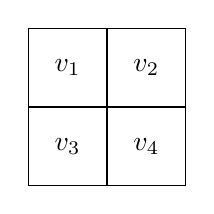
\begin{tikzpicture}[every node/.style={minimum size=1cm-\pgflinewidth, outer sep=0pt}]  
  \draw[step=1cm,color=black] (-1,-1) grid (1,1);
  \node at (-0.5,+0.5) {$v_1$};
  \node at (-0.5,-0.5) {$v_3$};
  \node at (+0.5,+0.5) {$v_2$};
  \node at (+0.5,-0.5) {$v_4$};
\end{tikzpicture}
\end{figure}

If you don't know anything at all, then all bets are off --- you could
be in any of the worlds $v_1,v_2,v_3,v_4$.  Furthermore, if you only
know a tautology, say $P\vee\neg P$, then you could be in any world.
That's what it means to say that tautologies are empty or contentless:
they don't rule out any possibilities.  If, in contrast, you know that
$P$, then you know that you're not in one of the bottom two worlds.
Hence, the proposition $P$ can be represented by graying the bottom
row.
\begin{figure}[h]
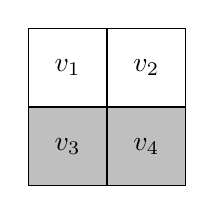
\begin{tikzpicture}[every node/.style={minimum size=1cm-\pgflinewidth, outer sep=0pt}]
    \draw[step=1cm,color=black] (0,-1) grid (2,1);
    \node[fill=gray!50] at (+0.5,-0.5) {$v_3$};
    \node[fill=gray!50] at (+1.5,-0.5) {$v_4$};
    \node at (+0.5,+0.5) {$v_1$};
    \node at (+1.5,+0.5) {$v_2$};
\end{tikzpicture}
  \caption{The proposition $P$ rules out possibilities $v_3$ and $v_4$.}
\end{figure}
Similarly, the proposition $Q$ can be represented by graying out the
column on the right; the proposition $\neg P$ can be represented by
graying out the top row; and the proposition $\neg Q$ can be
represented by graying out the column on the left.

Interestingly, this visual representation indicates that there are
``missing propositions'' that are of the same logical kind as $P$ and
$Q$ --- that is, other propositions that gray out two squares.
Consider, for example, the case where the top-right and bottom-left
square are grayed out.  The corresponding proposition $\phi$ doesn't
rule out $P$, and it doesn't rule out $Q$, and it doesn't rule out
either $\neg P$ or $\neg Q$.  What it does rule out are the
cross-cases where $P$ is true and $Q$ is false; and when $P$ is false
and $Q$ is true.  In other words, $\phi$ demands that $P$ have the
same truth-value as $Q$.  We see then that the proposition $\phi$
isn't missing after all: it's the proposition $P\lra Q$.

Propositions like $P$ and $Q$ leave open more than one possibility.
The tautologies, such as $P\vee\neg P$ leave open all possibilities;
and the contradictions, such as $P\wedge\neg P$ leave open no
possibilities (i.e.\ they cannot be true).  Another interesting kind
of proposition are those maximally specific propositions that leave
open only one possibility.  In this case, there are four maximally
specific propositions, represented by
$P\wedge Q,P\wedge\neg Q,\neg P\wedge Q$, and $\neg P\wedge\neg Q$.
\begin{figure}[h]
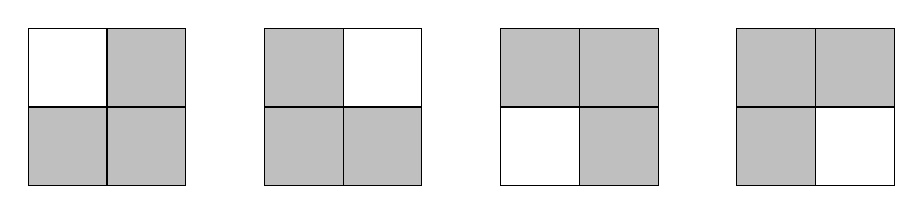
\begin{tikzpicture}[every node/.style={minimum size=1cm-\pgflinewidth, outer sep=0pt}]
    \draw[step=1cm,color=black] (-1,-1) grid (1,1);
    \node[fill=gray!50] at (-0.5,-0.5) {};
    \node[fill=gray!50] at (+0.5,+0.5) {};
    \node[fill=gray!50] at (+0.5,-0.5) {};
    \draw[step=1cm,color=black] (2,-1) grid (4,1);
    \node[fill=gray!50] at (+2.5,+0.5) {};
    \node[fill=gray!50] at (+2.5,-0.5) {};
    \node[fill=gray!50] at (+3.5,-0.5) {};
    \draw[step=1cm,color=black] (5,-1) grid (7,1);
    \node[fill=gray!50] at (+5.5,+0.5) {};
    \node[fill=gray!50] at (+6.5,-0.5) {};
    \node[fill=gray!50] at (+6.5,+0.5) {};
    \draw[step=1cm,color=black] (8,-1) grid (10,1);
    \node[fill=gray!50] at (+9.5,+0.5) {};
    \node[fill=gray!50] at (+8.5,-0.5) {};
    \node[fill=gray!50] at (+8.5,+0.5) {};
  \end{tikzpicture}
\caption{A $4\times 4$ square represents the space of all possible
  worlds.  Each coloring of a $4\times 4$ square represents a
  proposition, where the grayed-out squares are those worlds that the proposition rules
  out.  A maximally specific, consistent proposition rules out all
  worlds but one.} \end{figure}

We can also use these diagrams to understand better how the logical
connectives work.  For example, suppose that I assert:
\[ (P\wedge Q)\vee (P\wedge \neg Q) .\] The first disjunct permits
only world $v_1$, and the second disjunct permits only world $v_2$.
However, as I've asserted a disjunction, I've permitted either $v_1$
or $v_2$.  Hence the proposition $\phi$ I've asserted leaves the top
row open, i.e.\ $\phi$ must be equivalent to $P$.

If you think through all the possible ways of graying-out some subset
of possible worlds, you will quickly see that in one sense, there are
only $16$ distinct propositions.  There is one proposition that rules
out all worlds; and one that allows all worlds.  There are four
propositions that permit only one world.  There are also four
propositions that exclude only one world.  And then there are the six
propositions that permit exactly two worlds.  Of course, each of these
propositions can be represented by many different sentences --- e.g.\
$P$ and $P\wedge (Q\vee\neg Q)$ represent the same proposition.  But
it's good to know that every sentence represents one and only one of
these propositions.

Before concluding this discussion, we need to warn you about one
thing.  The preceding considerations might make it seem obviously true
that for each possible world $w$, there is a maximally specific
proposition that is true in $w$ and that is false at all other worlds.
While that is the case when there are only finitely many atomic
sentences, it can fail if there are infinitely many --- at least if
your propositions are themselves finite strings of symbols.  For if a
sentence $\phi$ contains only finitely many symbols, then there might
be an atomic sentence $X$ that doesn't occur in $\phi$.  Then, for any
world $w$ in which $\phi$ is true, there will be a distinct world $w'$
in which $\phi$ is also true, and in which the truth-value of $X$ is
flipped.  Thus, for a language with infinitely many atomic sentences,
there are no maximally specific propositions --- i.e.\ every
proposition is consistent with many different possibilities.

In the case where there are no maximally specific propositions, the
study of the collection of all possible worlds becomes more
mathematically rich.  In fact, there is a entire branch of mathematics
--- known as {\it topology} --- that studies collections like this,
with certain special subcollections, i.e.\ our propositions, which
topologists call ``neighborhoods.''

%% might do better to use coloring to *rule out* possibilities

%% briefly mention probability as a generalization of this -- and give
%% pointer to a book

%% TO DO: explain how one-block colorings are more contentful than multi

\begin{exercises} \mbox{}
  \begin{enumerate}
  \item Consider two arbitrary sentences that contain only the atomic
    sentences $P$ and $Q$.  Explain visually the relation between the
    colorings for $\phi$ and $\psi$ when $\phi$ logically implies
    $\psi$. 
\item Explain visually the relation between the colorings for $\phi$
  and $\psi$ when $\phi$ is inconsistent with $\psi$.
\item Use the method of coloring to show that
  $(P\lra Q)\vee (P\lra \neg Q)$ is a tautology.  Try to use the same
  thinking to construct an efficient formal proof of the sentence.
\item Let $P$ be any sentence that you wish or hope is true.  Here's
  how to prove that $P$ is true: let $\phi$ be the sentence ``if
  $\phi$ is true, then $P$.''  Show that $\phi$ is true, and hence
  that $P$ is true.  (Obviously something fishy is going on
  here!)  \end{enumerate} \end{exercises}


%%% Local Variables:
%%% mode: latex
%%% TeX-master: "main"
%%% End:


\chapter{Quantifying}

The following argument is  intuitively valid.
\[ \begin{array}{p{3.5cm}}
    All people are mortal. \\
    Socrates is a person. \\ \hline Socrates is mortal. \end{array} \]
However, the validity of this argument cannot be established by the
methods we developed in the previous chapters.  In particular, in this
argument, none of the sentences is logically complex --- i.e.\ none of
them is a conjunction, or a disjunction, or a conditional, or a
negated sentence.  Hence, the proper symbolization of this argument
would be $P,Q\vdash R$.  That sequent is invalid.  Therefore the
methods of the previous chapters would lead you to say that the
argument about Socrates is invalid.  Apparently the methods of the
previous chapters get this one wrong.\footnote{For the \"uber-critical
  reader: you might translate ``all people are mortal'' as a very long
  conjunction, and then the argument would show itself to be valid.
  We would reply to your objection by presenting an argument with a
  premise about all natural numbers.}

Here's another intuitively valid argument.
\[ \begin{array}{p{6.5cm}} Professor Dumbledore believes in magic.  \\
    \hline Some professors believe in magic.  \end{array} \] Again, by
the lights of propositional logic, the premise and conclusion of this
argument are \glspl{atomic sentence}.  Hence, the argument should be
symbolized as $P\vdash Q$, which is invalid.

We are going to move forward with the assumption that the above
arguments are valid.  To see {\it why} they are valid, we need a
deeper analysis than that provided by propositional logic.  As before,
the most important clue is the appearance of certain special words and
phrases that connect the ``content words'' in the argument.  In the
first argument, the key connecting word is ``all'', as we can see by
replacing the content words (person, mortal, Socrates) with letters.
\[ \begin{array}{p{3cm}}
     All $P$ are $M$. \\
     $s$ is $P$. \\ \hline Therefore, $s$ is $M$. 
   \end{array} \]  If you replace these letters with any grammatically suitable words,
 you'll find that the result is once again a good argument.  That's a
 sign that we've identified a valid argument form.  The next step then
 is to decide how to deal with the word ``all.''  Our previous logic words
 (and, or, if\dots then, not) played the role of sentence connectives:
 they construct new sentences out of old ones.  The word ``all'' plays
 a different role.  Here it seems to transform two predicate phrases
 (``\dots is a person'' and ``\dots is mortal'') into a sentence.  It
 doesn't make any sense to think of
 ``all'' as combining these phrases
 in the same way that, say, ``and'' combines two sentences.  

To see how ``all'' works, let's take a quick detour through another
argument.  
\[ \begin{array}{p{7.5cm}}
  If Socrates is a person then Socrates is mortal. \\
  Socrates is a person. \\ \hline
  Therefore, Socrates is mortal. \end{array} \] 
This argument {\it is} valid in respect to its propositional form
-- it's just an instance of modus ponens.  However, propositional
logic would have us use two completely different letters for
``Socrates is a person'' and ``Socrates is mortal'', thereby losing
track of the fact that those two sentences have the same subject.  So
now let's write $Ps$ for ``Socrates is a person'', and $Ms$ for
``Socrates is mortal''.  Then the argument would be symbolized as:
\[ \begin{array}{l}
Ps\to Ms \\
Ps \\ \hline 
Ms \end{array} \] 
Keeping your eye on the first premise $Ps\to Ms$, return now to the
question of how to represent the logical form of ``all persons are mortal.''
Let's remove the name Socrates, and replace it with a
place holder.  We'll use the letter ``$x$'' as our place holder.  Then
we get ``if $x$ is a person, then $x$ is mortal'' ($Px\to Mx$), which isn't exactly
a sentence, but which can be used to create sentences by plugging a
name in for $x$.  If we plug in $s$, we get the sentence $Ps\to Ms$.
Now, the sentence ``all $P$ are $M$'' says that no matter what name we
plug in for $x$, the resulting sentence is true, i.e.\ $Pa\to Ma$ is
true, and $Pb\to Mb$ is true, etc.  Thus, the first premise of our
original Socrates argument can be partially symbolized as:
\[ \begin{array}{p{8cm}}
     For any $x\:$ $(Px\to Mx)$ \end{array} \]
Now let's replace ``For any $x$'' with a symbol $\forall x$, yielding
the following symbolization of the original argument.
\[ \begin{array}{l}
     \forall x(Px\to Mx) \\
     Ps \\ \hline Ms \end{array} \] This argument form is valid, and we might want to add it as a
 basic rule.  But that would be a little short-sighted, because it
 wouldn't capture the full logical power of the concept represented by
 $\forall x$.  For example, the following argument form is also valid:
 \[ \begin{array}{l} \forall x(Fx\wedge Gx) \\ \hline \forall
     xFx \end{array} \] That is, if everything is both $F$ and $G$,
 then everything is $F$.  That's another obviously valid argument,
 indicating that $\forall x$ occurs in many different valid argument
 forms.  Our goal is to find the most basic valid inferences using
 $\forall x$, and then to show that these intuitively valid arguments
 -- and all others -- can be reconstructed from those basic valid
 inferences.

The newly introduced symbol $\forall x$ will be called the
\gls{universal quantifier}.  We used symbol $x$ as our placeholder,
and will call it a \gls{variable}, but that doesn't mean that any
``varying'' is happening here.  It's just a symbol.  We will also
sometimes use other letters at the end of the alphabet for variables,
and it will be important sometimes to have more than one variable in
play.  Suppose for example you want to represent the following
intuitively valid argument:
\[ \begin{array}{p{8cm}} 
  $\forall x$($\,x$ is divisible by $a$ $\,\to\,$ $x$ is divisible by $b\,$) \\
     $c$ is divisible by $a$ \\ \hline
     $c$ is divisible by $b$
   \end{array} \]
Here ``$x$ is divisible by $y$'' is a relation that holds between two
things, rather than a property of a single thing.  To represent ``$x$
is divisible by $y$,'' we can use a symbol such as $Dxy$ that has two
variables.  Then we can represent the preceding argument as follows:
\[ \begin{array}{l}
     \forall x(Dxa\to Dxb) \\
     Dca \\ \hline Dcb \end{array} \] We will also need our inference
 rules for $\forall x$ to explain why this argument is valid.  But before we get to that, we need to discuss another special logical notion that plays a key role in many valid arguments.

The following argument is intuitively valid.
\[ \begin{array}{p{6cm}}
     All Harvard graduates are hilarious.  \\
     Some Harvard graduates are felons.  \\ \hline
     Some felons are hilarious.  \end{array} \]
Here the first premise is again a universally quantified
  sentence.  But the second premise and the conclusion don't say that
{\it all} things have some feature; instead, they say that {\it some}
things have that feature.  We introduce a new symbol $\exists$
corresponding to the phrase ``There are some \dots '', and hence we
symbolize ``There are some things with feature $F$'' as $\exists
xFx$.  In the second premise we say that there are things that are
both Harvard graduates ($Hx$) and felons ($Fx$); hence it could be
symbolized as $\exists x(Hx\wedge Fx)$.  

The symbol $\exists x$ is called the \gls{existential quantifier}
because it expresses that something exists.  Like its universal
brother, it's always used with some particular variable which connects
it to the predicate or relation symbols that follow it.  Read somewhat
literally, $\exists xFx$ says that ``There is an $x$ such that $Fx$.''
Similarly, $\exists x(Fx\wedge Gx)$ says that ``There is an $x$ such
that $Fx$ and $Gx$.''

In English we have many phrases that express that something of a
certain sort exists.  We can say, ``there is \dots '' or ``there are
some \dots '' or ``something is \dots '', and many more like those.
In specific conversational contexts, these phrases can have more
specific implications --- e.g.\ they can indicate that there is more
than one, or that there are some things with this feature and some
things without it.  Consider, for example, if somebody asked your
logic professor ``do you have good students?''  If he answered, ``some
of them are good,'' then his interlocutor would reasonably conclude
that, in addition, some of them are not good.  That's because we are
often expected to answer by making the (logically) strongest statement
that we would be warranted in asserting.  If, in fact, your professor
believes that all his students are good, then why wouldn't he have
said that?

Similarly, suppose that your professor believes that only one student
in his class (of say $280$ students) is good, and that the rest of
them are terrible.  If he then says that ``some of my students are
good,'' one might justly accuse him of concealing the true situation.
He could just as easily say, ``strangely, only one of them is good.''
So, in that case, the phrase ``some'' wouldn't supply the most
accurate answer to the question.

Nonetheless, in symbolic logic, the existential quantifier has no
nuanced connotations.  The sentence ``$\exists xFx$'' simply means
that there is at least one $F$.  That's consistent with there being
only one $F$, or there being forty two $F$s, or with everything being
$F$.  If you wish that symbolic logic could be more nuanced, just
remember that what it loses in nuance it gains in clarity and rigor.

We've seen so far that we can express ``there is an $F$'' with
$\exists xFx$, and we can express ``some $F$ are $G$'' with
$\exists x(Fx\wedge Gx)$.  In a similar fashion, we can express ``some
$F$ are not $G$'' by $\exists x(Fx\wedge\neg Gx)$.  For example, to
say ``some Wall Street bankers are not evil,'' we could write
$\exists x(Wx\wedge\neg Ex)$.  Combining the expressive power of the
existential quantifier with that of the universal quantifier, we can
express the four standard sentence types that you might have seen
before in reference to Venn diagrams (Figure \ref{venn}).

\def\firstcircle{(1.5,0) circle (0.6cm)}
\def\secondcircle{(1.5,0) circle (1cm)}

\colorlet{circle edge}{black}
\colorlet{circle area}{gray!20}

\tikzset{filled/.style={fill=circle area, draw=circle edge, thick}, outline/.style={draw=circle edge, thick}}

\begin{figure}[h] \label{venn} \caption{The four standard types of quantified statements}
\centering
% Set A and B

\begin{tikzpicture}[every text node part/.style={align=center}]
\draw[filled] \firstcircle node { $F$ };
\draw \secondcircle node { };
\node[anchor=south,rectangle] at (current bounding box.north) { All $F$ are $G$ \\ $\forall x(Fx\to Gx)$};
\node at (2.1,0.6) { $G$ };
% \draw (-2.5,-2.5) rectangle (4.5,2.5) node [text=black,above] {$\emptyset$};
\draw (5,0) circle (1cm) node { $F$ };
\draw (7.5,0) circle (1cm) node { $G$ };
\node[anchor=south,rectangle] at (6.25,1) { No $F$ are $G$ \\ $\forall x(Fx\to \neg Gx)$};
\end{tikzpicture}
\end{figure}

\begin{figure}
\centering
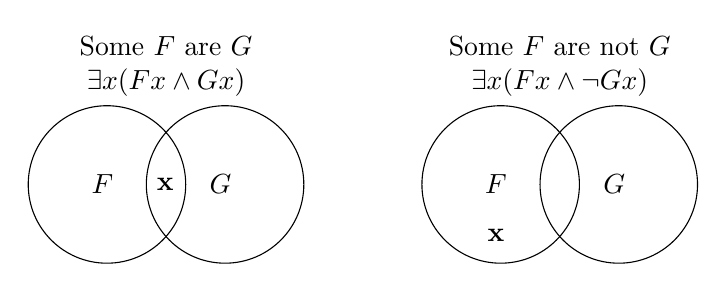
\begin{tikzpicture}[every text node part/.style={align=center}]
\draw (0,0) circle (1cm) node { $F$ };
\draw (1.5,0) circle (1cm) node { $G$ };
\draw (0.8,0) node { \textbf{x} };
\node[anchor=south,rectangle] at (0.75,1) { Some $F$ are $G$ \\ $\exists x(Fx\wedge Gx)$};
\draw (5,0) circle (1cm) node { $F$ };
\draw (6.5,0) circle (1cm) node { $G$ };
\draw (5,-0.65) node { \textbf{x} };
\node[anchor=south,rectangle] at (5.75,1) { Some $F$ are not $G$ \\ $\exists x(Fx\wedge \neg Gx)$};
\end{tikzpicture}
\end{figure}
                                                    

                                                    
                                                    
A common mistake that many beginning logic students make is to use $\exists x(Fx\to
Gx)$ for ``some $F$ are $G$''.  But a moment's thought shows that the
former symbolic sentence would be a bad translation.  The formula
$Fx\to Gx$ can be true of an individual $a$ for two different reasons.
First, $Fa\to Ga$ would be true if $Fa$ and $Ga$ are true.  But $Fa\to
Ga$ would also be true if $Fa$ were false.  (Just remember negative
paradox, or the truth-table for the conditional.)  Thus, $\exists
x(Fx\to Gx)$ would be true whenever something is not $F$, which fails
to capture the intent to assert the existence of something that is
both $F$ and $G$.

Similarly, it's easy to mistakenly write $\forall x(Fx\wedge Gx)$ when
you mean to say that ``all $F$ are $G$''.  But the sentence
$\forall x(Fx\wedge Gx)$ is way too strong: it says that everything
whatsoever is {\it both} $F$ {\it and} $G$.  Yes, it implies that all
$F$ are $G$, but only for the trivial reason that everything has both
features.  

As a general rule of thumb, if a natural language sentence is
translated to a universally quantified sentence, then the formula
inside the quantifier will be a conditional.  In contrast, if a
natural language sentence is translated to an existentially quantified
sentence, then the formula inside the quantifier will be a
conjunction.

%% exercises

\begin{exercise} Represent the form of the following sentences in
  predicate logic.  We've suggested appropriate symbols.  (For the
  sentences about people, you don't need to add an extra predicate for
  ``$x$ is a person.'')
  \begin{enumerate}
  \item No logicians are celebrities.  ($Lx,Cx$)
  \item Some celebrities are not logicians. ($Lx,Cx$)
  \item Only students who do the homework will learn logic.
    ($Sx,Hx,Lx$)
  \item All rich logicians are computer scientists. ($Rx,Lx,Cx$)
  \item All students and professors get a discount. ($Sx,Px,Dx$)
  \item No logician is rich, unless she is a computer
    scientist. ($Lx,Rx,Cx$)
  \item Not all logicians are computer scientist.  ($Lx,Cx$)
  \item Some logicians are rich computer scientists.  ($Lx,Rx,Cx$)
  \item If there are rich logicians, then some logicians are computer
    scientists. ($Rx,Lx,Cx$)
  \item No pets except service animals are permitted in dorms. ($Px,Sx,Dx$)
  \item If anyone is rich, then Mary is.  ($Rx,m$)
  \end{enumerate}
\end{exercise}

When you're symbolizing sentences, there will occasionally be cases
where there seem to be two (or more) possible correct answers.
Consider, for example, the sentence ``There are no friendly cats.''
If we use $Fx$ for ``$x$ is friendly'' and $Cx$ for ``$x$ is a cat'',
then any one of the following is a plausible representation of this
sentence:
\[ \neg\exists x(Fx\wedge Cx) \qquad \forall x(Fx\to \neg Cx) \qquad
  \forall x(Cx\to\neg Fx) \] The first sentence says that it's false
that there is a friendly cat.  The second sentence says that every
friendly thing is not a cat.  The third sentence says that every cat
is not friendly.  In English, these three statements have slightly
different connotations, and yet they would be true in precisely the
same circumstance, viz.\ the circumstance when the class of friendly
things does not include any cats.  Not long from now, you'll be able
to prove that these three sentences are in fact logically equivalent.

There are other cases where a natural language sentence is simply
ambiguous between two different ways that we might construe it in
symbolic language.  Consider, for example, the following
sentence:\footnote{This example was concocted by the logician Peter
  Geach (1916--2013).}
\begin{quote} Every boy loves a certain girl. \end{quote} Translating
this sentence might seem straightforward.  First, the sentence says
that every boy has a certain property, hence
$\forall x(Bx\to \phi (x))$, where $\phi (x)$ expresses ``$x$ loves a
certain girl''.  For the latter, we could write
$\phi (x)\equiv\exists y (Gy\wedge Lxy)$, which says that ``there is a
girl whom $x$ loves''.  The final answer then would be
\[ \forall x(Bx\to \exists yLxy ) .\] However, there's another way to
interpret this sentence: it might mean that there is some one girl who
is loved by every boy.  In that case, we want to approach the sentence
the other way around, i.e.\ we write $\exists y(Gy\wedge \psi (y))$,
where $\psi (y)$ expresses ``every boy loves $y$''.  Thus,
$\psi (y)\equiv \forall x(Bx\to Lxy)$, and the final answer is
\[ \exists y(Gy\wedge \forall x(Bx\to Lxy)) .\] Unlike the previous
example where the different translations were equivalent, these two
symbolic sentences are inequivalent --- they represent genuine
ambiguity in the initial English sentence.  In particular, it's
possible for the first sentence to be true while the second sentence
is false.\footnote{While it's intuitively clear that the first
  sentence does not imply the second, you'll first learn to prove that
  in Chapter \ref{inter}.}

The preceding considerations show that, in general, it makes a
difference which order you write quantifiers.  In fact, a famous
philosophical debate turns precisely on this point.  Among the many
attempts to prove God's existence, the so-called cosmological argument
begins from the premise that every event has a cause.  It then
concludes that there must be a first cause (which, the arguer
suggests, we can call ``God'').  If we were to try to capture the
argument in symbolic logic, then we might write the premise as
$\forall x\exists yRyx$, where $Ryx$ means that ``$y$ causes $x$''.
In that case, the conclusion would be represented as
$\exists y\forall xRyx$.  However, the philosopher Bertrand Russell
pointed out that the inference
$\forall x\exists yRyx\vdash \exists y\forall xRyx$ is {\it not}
valid.\footnote{The Russell-Copleston debate of 1948.  An audio
  recording of the debate can be found on the internet.}  Indeed, if
it were valid, then it would remain so no matter how we interpreted
the symbol $Ryx$.  But if we interpret $Ryx$ to mean that ``$y$ is the
mother of $x$'', then the premise is true of mammals, whereas the
conclusion is most definitely not true of mammals.

%% TO DO: introduce relation symbols

\begin{exercises} Represent the form of the following sentences in
  predicate logic.  We've suggested appropriate symbols.  (For the
  sentences about people, you don't need to add an extra predicate for
  ``$x$ is a person''.)
  \begin{enumerate}
  \item Mary loves everyone who loves her. ($m,Lxy$)
  \item Mary loves all and only those people who don't love
    themselves. ($Lxy,m$)
  \item Everyone loves their mother.  ($Lxy,Mxy$)
  \item Some people love only those people who love their
    mother. ($Lxy,Mxy$)
   \item Snape killed someone. ($Kxy,s$)
  \item Snape is a killer.  ($Kxy,s$)  
  \item Someone was killed by Snape. ($Kxy,s$)
  \item Some wizards only marry other wizards.  ($Wx,Mxy$) 
  \item There is no greatest number. ($Nx,x<y$)
  \item $c$ is the least upper bound of $a$ and $b$.  ($a,b,c,x\leq y$)
  \item $c$ is the greatest common divisor of $a$ and $b$.
    ($a,b,c,Dxy,x\leq y$)
   \end{enumerate} \end{exercises}


\section*{Universal Elimination}

We gave a big hint above about the meaning of $\forall x$.  We said
that somebody who accepts $\forall x\phi (x)$ would be willing to
grant that $\phi (a)$, no matter what $a$ names.  If that's right,
then the first and most obvious inference rule for quantified
statements should look like this:
\begin{quote} From $\forall x\phi (x)$, it's permitted to infer
  $\phi (a)$, for any name $a$. \end{quote} This rule will be called
\emph{universal elimination (UE)} since it permits us to infer
something from a universally quantified sentence.  Here we used the
notation $\phi (x)$ to stand for any formula that contains the
variable $x$.  For example, $\phi (x)$ could be $Px\to Mx$, or it
could be $Px\to Ms$, or it could be $Rx$.

The UE rule can be applied to prove $Ms$ from the conjunction of
$\forall x(Px\to Mx)$ and $Ps$.
\[ \begin{array}{l l >{$}p{3cm}<{$} p{1.5cm}}
  1 & (1) & \forall x(Px\to Mx) & A \\
  2 & (2) & Ps & A \\
  1 & (3) & Ps\to Ms & 1 UE \\
  1,2 & (4) & Ms & 3,2 MP \end{array} \]
Universal elimination (UE) is one of those simple rules of inference
where we carry down the dependency numbers of the sentence we use.  In
the above argument, we apply UE to line 1, which depends only on
itself.  Thus, the resulting line, i.e.\ line 3, also depends on just
line 1.

Here's the precise formulation of the UE rule.
\bigskip \begin{tcolorbox}[enhanced,width=10cm,title=Universal Elimination (UE),attach boxed title to top
  left={yshift=-2mm,xshift=4mm},boxed title style={sharp corners}]
From a universal sentence, you can infer any instance.  Schematically:  
$\begin{array}{l l}
     \Gamma\:\vdash\:\forall x\phi (x) \\
     \hline
     \Gamma\:\vdash\:\phi (a) \end{array} $
\end{tcolorbox} \bigskip

%% Now UE exercises

\begin{exercises} Prove the following sequents.
\begin{enumerate}
\item $\forall xFx,\forall xGx\:\vdash\: Fa\wedge Ga$
\item $\forall x\neg Fx\:\vdash\: Fa\to P$
\item $\forall x(Fx\to Gx),\neg Ga\:\vdash\:\neg Fa$
\item $\forall x(Fx\to Gx),\neg Ga\:\vdash\:\neg \forall xFx$  
\item $\forall x\neg Fx\:\vdash\:\neg\forall xFx$
\item $\vdash\:\neg\forall x(Fx\wedge\neg Fx)$
\end{enumerate}
\end{exercises}

\begin{exercise} Do the sentences $\forall x(Fx\to Gx)$ and
  $\forall x(Fx\to \neg Gx)$ seem consistent to you? \end{exercise}



\section*{Universal Introduction}

The UE rule won't do much for you on its own.  For example, if you're
trying to infer $\forall xFx$ from $\forall x(Fx\wedge Gx)$, UE can
take you down to $Fa\wedge Ga$, but it can't get you back up to
$\forall xFx$.  Indeed, to infer a universal sentence from any
particular instance is the worst kind of mistake.  For example, you
cannot conclude that all professors believe in magic from the fact
that Professor Dumbledore believes in magic.  Thus, in order to get
the most out of the UE rule, it needs to be supplemented with a
universal introduction rule.

Recall that conditional proof isn't just a rule, it's a strategy for
thinking.  In short, if you want to prove a conditional, then your
first move is to assume the antecedent, which you can use in reasoning
toward the consequent.  Now, universal introduction (UI) will be like
conditional proof in this regard.  Only now we have to think about
how we come to be convinced of the truth of universal statements.

It is really quite amazing that human beings can ever come to know
that a universal statement is true.  We are limited in space and time,
and none of us will ever be able to survey all possible instances of
any generalization.  So what could permit us -- who can only observe
a small finite number of instances -- to conclude that something is
always true?

The answer is similar to the one we gave for conditional statements.
To reason to a conditional statement, we engage in the mental activity
of {\it supposing}, an activity that is not itself aimed at telling
the truth.  When I say ``suppose that $P$,'' I am not making a claim
about what is the case; instead, I'm abstracting away from reality so
that I can explore logical connections.  When it comes to
establishing universal claims, we engage in an even more radical
version of abstraction.  In essence, we suppose that we can talk about
things in general, without talking about any particular thing.

Consider the following dialogue where A and B agree that all Bavarians
are German, and all Germans are European, and A is trying to convince
B that all Bavarians are European.

\begin{quote} A: Suppose that Gretel is some random Bavarian. \newline
  B: So the random Bavarian is female?  \newline
  A: No, I didn't mean that at all.  I just meant to choose a
  Bavarian-sounding name.  If I had chosen ``Hansel,'' you might have
  asked me if the random Bavarian is male. \newline
  B: Why don't you just use a letter then? \newline
  A: OK, suppose that $X$ is some random Bavarian.  
  You agree with me then that $X$ is German, right?  \newline
  B: Yes, certainly.  \newline
  A: And since all Germans are European, $X$ is European.
  \newline
  B: Agreed. \newline
  A: Since $X$ was an arbitrary Bavarian, it follows that every Bavarian is European.  \end{quote}

It's this last step where all the action happens.  The letter $X$
plays the role of name, but we don't know anything about who it names
-- except that he or she is Bavarian.  So, when we deduce that $X$ is
European, that licenses us to conclude that {\it all} Bavarians are
Europeans.

We have to beware of a danger here.  In the above dialogue, the two
parties chose the letter $X$ because there was little danger that the
letter would carry connotations that would derail their reasoning
process.  But there are no guarantees.  What if B were obtuse, like this.
\begin{quote}
  B: Since the arbitrary Bavarian's name is ``$X$'', it follows that no
  Bavarians have the name ``Gretel.'' \end{quote} Obviously, something
has gone very wrong with B's thinking about these issues.
Essentially, B forgot that the whole point of choosing a letter ``$X$''
was so that nobody would assume they know anything about $X$.  But
that's exactly what B has done, she has assumed that $X$ has the
feature that its name is ``$X$''.  She has missed the point
completely.

In real-life reasoning, people have common sense to prevent them from
making such mistakes.  But the goal of formal logic is to make
explicit the rules that common sense suggests.  We want to forbid this
kind of mistake by means of an explicit rule, and here's how we'll do
it.

To use an analogy, suppose that the argument or dialogue takes place
in a closed room.  And suppose that when the two parties enter the
room, they each have to declare their assumptions.  Once the dialogue
begins, they can use those assumptions that they declared upon
entering the room.  When it comes to reasoning about universal claims,
we'll give both parties a stock of new names $a,b,c,\dots $, that do
{\it not} occur anywhere in their declared assumptions.  They may then
use these names at any point in their argument.  For example, they may
use UE to infer $\phi (a)$ from $\forall x\phi (x)$.

With these new regulations in place, we can prevent the parties from
making silly mistakes in deducing universal sentences.  In short, one
may infer a universal sentence $\forall x\phi (x)$ from an instance
$\phi (a)$ that contains one of the new names we supplied.  Since the
two parties didn't bring in any information about $a$, the only
information they can have about $a$ is what they have deduced from
universal statements.

Hopefully the analogy helps your intuition.  But you won't need the
intuition to follow the universal introduction rule, which provides a
simple (machine checkable!) syntactic recipe.  In short, UI allows you
to infer $\Gamma\vdash\forall x\phi (x)$ from $\Gamma\vdash \phi (a)$
whenever there is no information about $a$ in the background
assumptions $\Gamma$, or hidden in the formula $\phi (x)$.

\bigskip \begin{tcolorbox}[enhanced,width=10cm,title=Universal Introduction (UI),attach boxed title to top
  left={yshift=-2mm,xshift=4mm},boxed title style={sharp corners}]
\[ \begin{array}{r@{\; }c@{\; }l c@{\quad }p{6cm}}
       \Gamma & \vdash & \phi (a) & & \multirow{2}{6cm}{\small restriction: $a$ does not occur in $\Gamma$ or $\phi (x)$.} \\ \cline{1-3}
       \Gamma & \vdash & \forall x\phi (x) \end{array} \]  
 \end{tcolorbox} \smallskip

In general, universally quantified premises can be used together to
draw universally quantified conclusions.  The strategy is often as
simple as applying UE repeatedly to the premises, making sure to use
the same name in each case.  Then one uses the rules of propositional
logic to transform those instances to an instance of the conclusion.
Finally, one applies UI to infer the conclusion from that instance.

\medskip \noindent \textbf{To prove:} $\forall x(Fx\to Gx),\forall x(Gx\to Hx)\:\vdash\: \forall x(Fx\to Hx)$
\[ \begin{array}{l l >{$}p{3.5cm}<{$} p{2cm}}
     1 & (1) & \forall x(Fx\to Gx) & A \\
     2 & (2) & \forall x(Gx\to Hx) & A \\
     3 & (3) & Fa                  & A \\
     1 & (4) & Fa\to Ga            & 1 UE \\
     2 & (5) & Ga\to Ha            & 2 UE \\
     1,3 & (6) & Ga                & 4,3 MP \\
     1,2,3 & (7) & Ha              & 5,6 MP \\
     1,2 & (8) & Fa\to Ha          & 3,7 CP \\
     1,2 & (9) & \forall x(Fx\to Hx) & 8 UI \end{array} \] Looking at
 the conclusion, we realized that we need to show that an arbitrary $F$ is also an $H$.  That is, we need to show that $Fa\to Ha$, depending on no assumptions that mention $a$.  So then on line 3, we suppose that $a$ is an arbitrary $F$.  (There is nothing in line 3 that says ``is an arbitrary,'' but that effect is ensured by choosing a name $a$ that hasn't yet occurred in the proof.)  Then we proceed to use the universal premises to infer that $a$ is also an $H$.
 
 The restriction on the name $a$ corresponds to the idea that a fully
 general statement cannot be inferred from specific assumptions.  To
 see why we prohibit $a$ from occurring in $\phi (x)$, consider the
 following attempt to prove $\forall xRxa$ from $\forall xRxx$.
\[ \begin{array}{l l >{$}p{2cm}<{$} p{1cm} p{4cm}}
     1 & (1) & \forall xRxx & A \\
     1 & (2) & Raa          & 1 UE \\
     1 & (3) & \forall xRxa & 2 UI &
                                     $\Longleftarrow$
                                     incorrect \end{array} \] %
This argument cannot possibly be valid.  Suppose that $Rxy$ is the
relation ``$x$ has the same net worth as $y$'' and that $a$ is a name
for Jeff Bezos.  The premise is then obviously true: everybody has the
same net worth as themselves.  But the conclusion says that everyone
has the same net worth as Jeff Bezos, which is as far from the truth
as possible.  The problem here is line 3, since the formula $\phi (x)$
is $Rxa$, which contains the name $a$.  In practice, you can ensure
that you don't violate this restriction on UI if you follow this rule
of thumb: when generalizing $\phi (a)$ to $\forall x\phi (x)$, 
change all occurrences of $a$ to $x$. In the case at hand, that would
have forced us to generalize $Raa$ to $\forall xRxx$, which is just
what we started with.

% When you're trying to derive a universal conditional such as
% $\forall x(Fx\to Gx)$, then it makes sense to begin by assuming $Fa$,
% where $a$ is a new name.  You can then apply UE to any universal
% premises to try to get information that will allow you to derive $Ga$.
% In other cases, it makes sense just to start by applying UE to your
% premises, to see if they give you the conclusion you want.  For
% example, in the following proof, we need to show that an arbitrary
% thing if $F$.  For that, it would suffice to show that $Fa$ for an
% arbitrary $a$; and applying UE to line 1 yields $Fa\wedge Ga$.
% \[ \begin{array}{l l >{$}p{2.5cm}<{$} p{1.5cm}}
%      1 & (1) & \forall x(Fx\wedge Gx) & A \\
%      1 & (2) & Fa\wedge Ga & 1 UE \\
%      1 & (3) & Fa & 2 $\wedge$E \\
%      1 & (4) & \forall xFx & 3 UI \end{array} \] The use of UI on line
% 4 is permitted because line 3 depends only on 1, and the name $a$ does not occur in line 1.

%% TO DO: slightly more interesting use of UI

The UI rule can be used with any variable.  For example, $\phi (a)$
can be quantified to $\forall x\phi (x)$ or $\forall y\phi (y)$ or
$\forall z\phi (z)$.  You only need to make sure not to get yourself
confused by using a variable that already occurs in $\phi (a)$.  So,
for example, you wouldn't infer $\forall x\forall xRxx$ from
$\forall xRax$, because the former string of symbols doesn't make
sense as a formula.

Using the freedom to apply UI with any variable, it follows that
universal statements $\forall xFx$ and $\forall yFy$ are equivalent.
\[ \begin{array}{l l >{$}p{2.5cm}<{$} p{2cm}}
     1 & (1) & \forall xFx & A\\
     1 & (2) & Fa          & 1 UE \\
     1 & (3) & \forall yFy & 2 UI \end{array} \] The converse proof
 follows by symmetry, hence $\forall xFx\dashv\vdash \forall yFy$.
 These equivalences -- where one variable is switched throughout for
 another -- are known as $\alpha$-equivalences, and they can be really
 useful when dealing with sentences that contain more than one
 variable.  For example, by $\alpha$-equivalence, $\forall xFx\to
 \forall yFy$ is a tautology; and we'll soon see that $\forall xFx\to
 P$ implies $\exists x(Fx\to P)$.  Thus, substituting $\forall
 yFy$ for $P$ shows that $\exists x(Fx\to \forall yFy)$ is a tautology.

\begin{exercises} Prove the following sequents. \label{ex:ui}
  \begin{enumerate}
    \item $\forall x(Fx\to Gx)\:\vdash\: \forall xFx\to \forall xGx$
    \item $\forall x(Fx\to Gx)\:\vdash\:\forall x\neg Gx\to \forall
      x\neg Fx$
    \item $\forall xFx\wedge \forall xGx\:\dashv\vdash\: \forall x(Fx\wedge
      Gx)$
    \item $\forall xFx\vee \forall xGx\:\vdash\: \forall x(Fx\vee Gx)$
    \item $\neg Fa\:\vdash\:\neg\forall xFx$
    \item $\forall x\neg Fx\:\vdash\:\forall x(Fx\to Gx)$
    \item $P\:\vdash\: \forall x(Fx\to P)$, where $P$ is any sentence
      that doesn't contain the variable $x$.
    \item $P\to \forall xFx\:\dashv\vdash\: \forall x(P\to Fx)$  
    \item $\forall x\forall yRxy\:\vdash\: \forall xRxx$
    \item $\forall x\forall yRxy\:\vdash\: \forall y\forall xRxy$
    \end{enumerate}
  \end{exercises}

  \begin{exercise} What's wrong with the following attempted proof? 
\[ \begin{array}{l l >{$}p{3cm}<{$} p{1.5cm}}
     1 & (1) & Fa  & A \\
       & (2) & Fa\to Fa & 1,1 CP \\
       & (3) & \forall x(Fa\to Fx) & 2 UI  \\
       & (4) & Fa\to Fb & 3 UE \end{array} \] \end{exercise}

 \begin{exercise} Start to try to write a proof of \[ \forall x(Fx\vee
  Gx)\:\vdash\:\forall xFx\vee \forall xGx ,\] and explain where the
  restriction on UI prevents you from continuing. \end{exercise}  
  

\section*{Existential Introduction}

It's not too uncommon that we know that there is something or other
with a certain feature, but we don't know who or what it is that has
that feature.  For example, we know that somebody murdered eleven
women in London in the years 1888 to 1891, but as of today, the
identity of the murderer is still unknown.

We can also use such knowledge to infer other things, although we have
to be careful when using knowledge that ``something is $\phi$''
without knowing who or what it is that is $\phi$.  For example, if you
know that something is $\phi$, and you know that all $\phi$ are
$\psi$, then you also know that something is $\psi$.  In contrast, you
might know that something is $\phi$ and that something is $\psi$; but
those two facts do {\it not} entitle you to conclude that something is
both $\phi$ and $\psi$.

What then is the logic of ``something is $\phi$''?  As with our other
key logical notions, we are looking here for typical inferences to
such statements (an introduction rule), and typical inferences
from such statements (an elimination rule).

Let's look first for an existential intro rule -- i.e.\ a paradigmatic
inference to a statement of the form ``something is $\phi$.''  In real
life, our reasons for believing existential statements are frequently
not {\it guaranteeing} reasons, in the sense that the existential
statement is a logical consequence of what we know.  For example, in
the Jack the Ripper case, the reason that I believe that somebody
killed eleven women is because I read about it, or heard about it on
TV.  But of course, the documentary evidence doesn't guarantee -- in a
logical sense -- that the event actually happened.  So this kind of
evidence is not what we're looking for in a deductively valid rule of
existential introduction.

However, there was at least one person who had guaranteeing evidence
for the claim that someone killed eleven women.  In particular, Jack
the Ripper -- if he existed -- knew that ``I killed eleven women,''
and so he would have been entitled to infer that ``somebody killed
eleven women.''  There is {\it no way} that the premise could be true
and the conclusion false, indicating the presence of a valid argument
form.  Thus, Jack the Ripper's valid inference could be represented as
follows:
\[ \begin{array}{c} \phi (a) \\ \hline \exists x\phi
    (x) \end{array} \] Here $a$ is Jack's name for himself, and
$\phi (x)$ represents ``$x$ murdered eleven women.''  Thus, the
inference goes from ``I murdered eleven women'' to ``somebody murdered
eleven women.''  We'll take this inference to be the paradigm way that
an existential statement can be inferred from another statement.
\bigskip \begin{tcolorbox}[enhanced,width=10cm,title=Existential
  Introduction (EI),attach boxed title to top
  left={yshift=-2mm,xshift=4mm},boxed title style={sharp corners}] If
  an instance $\phi (a)$ of $\exists x\phi (x)$ follows from $\Gamma$,
  then $\exists x\phi (x)$ follows from $\Gamma$.  Schematically:
$\arraycolsep=1.4pt \begin{array}{r c l}     \Gamma & \vdash & \phi (a) \\
     \hline
     \Gamma & \vdash & \exists x\phi (x) \end{array} $
\end{tcolorbox} \bigskip
\noindent Here $\phi (x)$ is a formula in which the variable $x$ occurs, and
$\phi (a)$ is the formula that is obtained by replacing all the
instances of $x$ in $\phi (x)$ with $a$.  However, there is no requirement that $a$ does
{\it not} occur in $\phi (x)$.  For example, it's perfectly legitimate
to infer that somebody killed Ernest Hemingway from the fact that
Ernest Hemingway committed suicide.  That is, $\exists xKxa$ can be
inferred, by existential intro, from $Kaa$.  

Like disjunction intro, existential intro actually throws away
information -- and so it's dangerous to use it without knowing where
you want to go.  Remember that disjunction intro is most useful in
cases where you want to show that two different premises have the same
conclusion.  We'll soon see that the same sort of intuition applies to
existential intro, i.e.\ it's most effective in the search for a
common conclusion from several different premises. 

Nonetheless, there are some cases where EI by itself is useful.  In
the following we show that a negated existential sentence implies a
universal sentence. \label{qne}

\medskip\noindent\textbf{To prove:} $\neg\exists xFx\vdash\forall x\neg Fx$
\[ \begin{array}{l l >{$}p{4cm}<{$} p{2cm}}
     1 & (1) & \neg\exists xFx & A \\
     2 & (2) & Fa              & A \\
     2 & (3) & \exists xFx     & 2 EI \\
     1,2 & (4) & \exists xFx\wedge\neg\exists xFx & 3,1 $\wedge$I \\
     1   & (5) & \neg Fa     & 2,4 RAA \\
     1   & (6) & \forall x\neg Fx  & 5 UI \end{array} \]
(Note that since line 5 depends only on line 1, and line 1 does not
contain $a$, the invocation of UI on line 6 is legitimate.)  Here our
strategy is not completely straightforward.  The premise $\neg\exists
xFx$ is not in itself useful: it's a negated sentence, and none of our
rules will let us do something with a single negated sentence.  We
then have to work our way backwards from the conclusion, which is
$\forall x\neg Fx$.  Since it's a universal sentence, it would suffice
to obtain an instance $\neg Fa$, so long as that instance doesn't
depend on any assumptions about $a$.  In frustration, one might decide
(as we did) to try to obtain $\neg Fa$ by reductio ad absurdum.
Indeed, as soon as we assumed $Fa$, it was obvious that it conflicts
with the premise on line $1$.

Notice that if we run through the preceding proof, replacing $Fx$ with
$\neg Fx$, then line 5 would become $\neg\neg Fa$.  We can then perform a
step of DN elimination to get $Fa$, and then $\forall xFx$.  Thus, we also
have a proof of the sequent $\neg\exists x\neg Fx\vdash\forall xFx$.

% \[ \begin{array}{l l >{$}p{4cm}<{$} p{2cm}}
%      1 & (1) & \neg\exists x\neg Fx & A \\
%      2 & (2) & \neg Fa              & A \\
%      2 & (3) & \exists x\neg Fx     & 2 EI \\
%      1,2 & (4) & \exists x\neg Fx\wedge \neg\exists x\neg Fx & 3,1
%                                                                $\wedge$I
%      \\
%      1 & (5) & \neg\neg Fa  & 2,4 RAA \\
%      1 & (6) & Fa           & 5 DN \\
%      1 & (7) & \forall xFx  & 6 UI \end{array} \]

%% TO DO: explain clearly what counts as an INSTANCE

\begin{exercises} Prove the following sequents. \label{harder} \label{ex:ei}
  \begin{enumerate}
  \item $\neg\exists x (Fx\wedge Gx)\:\vdash\:\forall x(Fx\to \neg Gx)$
  \item $\forall xFx\:\vdash\:\exists xFx$    
  \item $\forall x(Fx\to Gx),Fa\:\vdash\: \exists xGx$
  \item $\neg Fa\:\vdash\:\exists x(Fx\to P)$
  \item $\neg\forall xFx\:\vdash\:\exists x(Fx\to P)$
  \item $\neg \exists xFx\:\vdash\:\forall x(Fx\to Gx)$    
  \item $\forall x\forall yRxy\:\vdash\:\exists xRxx$
  \item $P\to Fa\:\vdash\: P\to \exists xFx$
    % \item $P\to Fa\:\vdash\:\exists x(P\to Fx)$
    % \item $\neg\exists x\neg Fx\:\vdash\:\forall xFx$
  \item $\exists xFx\to P\:\dashv\vdash\:\forall x(Fx\to P)$    
  \item $\neg \exists xFx\:\vdash\:\forall x(Fx\to P)$
  \item $\neg \exists x(Fx\to P)\:\vdash\: \forall xFx\wedge\neg P$  
  \sitem $\forall xFx\to P\:\vdash\:\exists x(Fx\to P)$
   %% try RAA.  Assume Fa > P.  Get Fa & -P.   
 % forall xFx\:\vdash\: \exists x\neg Fx$
  \end{enumerate}
\end{exercises}

\section*{Existential Elimination}

%% TO DO: first existentials interacting, then existentials together
%% with universals

The real power of existential intro comes when it's combined with an
existential elimination rule.  But let's slow down, because existential
elimination is the most conceptually challenging rule in this book.

To understand the conceptual challenge of existential elimination,
let's first note what the rule could {\it not} be.  The following
inference is definitely invalid.
\[ \begin{array}{c} \exists x\phi (x) \\ \hline \phi
    (a) \end{array} \] For example, from the fact that somebody killed
eleven women, you cannot validly conclude that Lewis Carroll killed
eleven women.  

If you think about it, it's hard to see how one could derive anything
of interest from an existentially quantified statement.  The problem
is that $\exists x\phi (x)$ just doesn't tell you which thing is
$\phi$.  So, how can you {\it use} that statement when it is so
unspecific?  Well, the strategy here will be quite similar to the
strategy we used for UI.  The sentence $\exists x\phi (x)$ doesn't
tell us that Richard or Connie or Albert is $\phi$, but it tells us
that something is $\phi$.  So, you could then grab a new name $a$ off
the shelf, and use it for this $\phi$.  Then, you can explore logical
space, seeing what conclusions you can reach -- without assuming any
further knowledge about the identity of $a$.  The idea then is that
whatever conclusion $\psi$ you reach, as long as it doesn't mention
$a$, follows from $\exists x\phi (x)$.

For example, let's take it as given that somebody killed eleven women
in London between 1888 and 1891.  We can call this person ``Jack the
Ripper,'' or $a$ for short, and then we could start drawing
conclusions by means of standard logical reasoning.  We could infer
that $a$ was a serial killer in London in the late 1800s; and hence by
existential intro, that there was a serial killer in London in the
late 1880s.  Since that conclusion doesn't beg any questions about the
identity of the person, we have reliably deduced that there was a
serial killer in London in the late 1800s.  

That's how existential elimination will work.  In this case, let's use the rule before properly explaining it.  We
will derive $\exists xFx$ from the premise $\exists x(Fx\wedge Gx)$.
\[ \begin{array}{l l >{$}p{2.5cm}<{$} p{1.5cm}}
  1 & (1) & \exists x(Fx\wedge Gx) & A \\
  2 & (2) & Fa\wedge Ga & A \\
  2 & (3) & Fa & 2 $\wedge$E \\
  2 & (4) & \exists xFx & 3 EI \\
  1 & (5) & \exists xFx & 1,2,4 EE \end{array} \]
The first four lines use rules that you've seen before, but the second
line isn't deduced from the first, it's a new
assumption.  You might want to gloss line 2 as saying ``let $a$ be a
name for one of these things that is $F$ and $G$.''  Line 5 is where all the action happens.  Line 4 shows that
$Fa\wedge Ga\vdash \exists xFx$, and that conclusion would
have followed no matter what name $a$ we had chosen on line 2.  Thus,
$\exists xFx$ follows simply from the fact that {\it something} is $F$
and $G$, which is what allows us to replace the dependency on 2 with
dependency on 1 in line 5.  Here our EI rule cites three lines: line 1 where the existential sentence
occurs, line 2 where an instance of that sentence occurs, and line 4
where we've drawn a conclusion from that instance.  The second two
lines mark off a sub-proof, namely the derivation of
$\exists xFx$ from $Fa\wedge Ga$.  So, while EE officially cites three
lines, it's best to think of EE as citing one line (with an
existential sentence), and then a sub-proof that begins with an
assumption (of an instance of the existential) and that ends with the
desired conclusion.

Now we're ready for a fully precise description of the EE rule, along
with all of its restrictions.
\bigskip \begin{tcolorbox}[enhanced,width=11cm,title=Existential Elimination (EE),attach boxed title to top
  left={yshift=-2mm,xshift=4mm},boxed title style={sharp corners}]
  If an instance $\phi (a)$ of $\exists \phi (x)$ implies $\psi$, and the name $a$ does not occur in $\psi$, then $\exists x\phi (x)$ implies $\psi$.  More precisely, 
  \[ \begin{array}{c c@{\quad }p{4cm}}
       \Gamma \vdash \exists x\phi (x) \quad \Delta ,\phi (a) \vdash \psi & & \multirow{2}{4cm}{\small restriction: $a$ does not occur in $\Gamma$, $\Delta$, $\phi (x)$ or $\psi$.} \\ \cline{1-1}
       \Gamma ,\Delta \vdash \psi \end{array} \]
 \end{tcolorbox} \bigskip
 In this picture, we have three things:
 \begin{enumerate}
   \item A  derivation of $\exists
x\phi (x)$ from some premises $\Gamma$.  That corresponds to a line in
a proof on which an existential sentence occurs, with dependencies
$\Gamma$.
\item A derivation of $\psi$ from an instance $\phi (a)$, plus
  possibly some auxiliary assumptions $\Delta$.  These auxiliary
  assumptions cannot say anything about $a$.  In a proof, this
  derivation begins with an assumption of $\phi (a)$, and ends on a
  line with $\psi$ that depends on nothing but $\Delta$ and $\phi
  (a)$.
\item When the first two things are in place, we are permitted to
  infer $\psi$ by EE, where the dependencies are the union of $\Gamma$
  and $\Delta$. \end{enumerate}

Here's a simple example of all the different bits in play.

\medskip\noindent \textbf{To prove:} $\forall x(Fx\to Gx),\exists
xFx\vdash\exists xGx$
\[ \begin{array}{l l >{$}p{3cm}<{$} p{2cm}}
     1 & (1) & \forall x(Fx\to Gx) & A \\
     2 & (2) & \exists xFx         & A \\
     3 & (3) & Fa & A \\
     1 & (4) & Fa\to Ga & 1 UE \\
     1,3 & (5) & Ga     & 4,3 MP \\
     1,3 & (6) & \exists xGx & 5 EI \\
     1,2 & (7) & \exists xGx & 2,3,6 EE \end{array} \] Here our
$\Gamma$ is simply $\exists xFx$ itself, and the first part of the EE
is just line 2 (i.e.\ the derivation of $\exists xFx$ from itself).
The second part of the EE is the subproof that begins on line 3 (the
assumption of the instance $Fa$) and that ends on line 6 (the
conclusion $\exists xGx$).  This sub-proof shows $\forall x(Fx\to
Gx),Fa\vdash\exists xGx$, i.e.\ our auxiliary assumption $\Delta$
is simply $\forall x(Fx\to Gx)$.  All the restrictions on EE
are respected, and so line 7 is correct.

The legalistic restrictions on EE might seem hard to remember, but
they all flow from the same idea that an existential sentence $\exists
x\phi (x)$ doesn't give any information about who or what is $\phi$.
Of course, it would be blatantly invalid to argue from an existential
claim $\exists xFx$ to the claim that $Fa$.
\[ \begin{array}{l l >{$}p{2cm}<{$} p{2cm} p{3cm}}
     1 & (1) & \exists xFx & A & \\
     2 & (2) & Fa          & A & \\
     1 & (3) & Fa          & 1,2 EE & $\Longleftarrow$
                                      incorrect \end{array} \]
Here the application of EE on line $3$ violates the restriction that
the name $a$ may not appear in the conclusion of the subproof.  

In practice, the best way not to run afoul of the restrictions on EE
is to choose a completely new name $a$ for the assumed instance
$\phi (a)$, and then not to make any further assumptions about $a$.
The {\it only} fact that you should use about $a$ is that it is one
of the things that makes $\exists x\phi (x)$ true.  Consider, for
example, what would happen if we tried to derive $\exists x(Fx\wedge
Gx)$ from $\exists xFx$ and $\exists xGx$.
\[ \begin{array}{l l >{$}p{3cm}<{$} p{1.5cm} p{6cm}}
     1 & (1) & \exists xFx  & A \\
     2 & (2) & \exists xGx  & A \\
     3 & (3) & Fa           & A \\
     4 & (4) & Ga           & A & $\Longleftarrow$ bad idea \\
     3,4 & (5) & Fa\wedge Ga  & 3,4 $\wedge$I \\
     3,4 & (6) & \exists x(Fx\wedge Gx) & 5 EI  \end{array} \]
If we tried to perform EE on lines 1,3 and 6, we would have the
following setup:
\[ \begin{array}{c c}
     \exists xFx\:\vdash\:\exists xFx \qquad Ga,Fa\:\vdash\:\exists
     x(Fx\wedge Gx) \\ \hline
     \exists xFx,Ga\:\vdash\:\exists x(Fx\wedge Gx) \end{array} \]
The problem here is that the auxiliary assumption $\Delta$ is $Ga$,
which mentions something specific about $a$.  That's not allowed, so
lines 1,3, and 6 cannot be used for EE.

The problem with the preceding argument is clear if you just use some
common sense.  Suppose that you know someone who loves logic, and
someone else who hates logic.  Then it would be a bad idea to say
``suppose that $a$ loves logic,'' and in the next breath, ``suppose
that $a$ hates logic.''  There's nothing logically illegal with making
both suppositions -- logic places no restrictions on supposing things
-- but the logic police won't let you use these suppositions together
to infer something from an existential premise.

In Exercise \ref{ex:ui}, you showed that the universal quantifier commutes with
conjunction, that is
\[ \forall x(Fx\wedge Gx)\:\dashv\vdash\: \forall xFx\wedge \forall xGx . \]
While the existential quantifier doesn't commute with conjunction, it
commutes with disjunction.  We prove one direction here, and leave
the other to the exercises.

\medskip \noindent \textbf{To prove:} $\exists x(Fx\vee Gx)\:\vdash\: \exists
xFx\vee\exists xGx$
\[ \begin{array}{l l >{$}p{4cm}<{$} p{2cm}}
     1 & (1) & \exists x(Fx\vee Gx) & A \\
     2 & (2) & Fa\vee Ga            & A \\
     3 & (3) & Fa                   & A \\
     3 & (4) & \exists xFx          & 3 EI \\
     3 & (5) & \exists xFx\vee \exists xGx & 4 $\vee$I \\
     6 & (6) & Ga                   & A \\
     6 & (7) & \exists xGx          & 6 EI \\
     6 & (8) & \exists xFx\vee\exists xGx & 7 $\vee$I \\
     2 & (9) & \exists xFx\vee\exists xGx & 2,3,5,6,8 $\vee$E \\
     1 & (10) & \exists xFx\vee\exists xGx & 1,2,9 EE \end{array} \]
 It may seem strange that the sentence $\phi\equiv \exists xFx\vee\exists xGx$
 occurs four times in this proof.  However, in each case it occurs
 with different dependencies, and so it says something different.  The
 first instance, on line $5$, says that $\phi$ follows from $Fa$.  The
 second instance, on line $8$, says that $\phi$ follows from $Ga$.  Those two sub-derivations
 show that $\phi$ follows from the disjunction
 $Fa\vee Ga$, and since the name $a$ was arbitrary, $\phi$
 follows from the existential sentence $\exists x(Fx\vee Gx)$.

Some applications of existential elimination are a bit more subtle.
Consider, for example, the following derivation of $\neg\forall xFx$
from $\exists x\neg Fx$.  If you ignored the conclusion and tried to
extract some information from the premise, you wouldn't get very far.
Being an existential sentence, the premise is weak.  However, since
the conclusion is a negated sentence $\neg \phi$, it makes sense to
assume $\phi$ and to try for reductio ad absurdum. That's what we've
done here. \label{argh}

\medskip \noindent \textbf{To prove:} $\exists
x\neg Fx\vdash\neg\forall xFx$
\[ \begin{array}{l l >{$}p{2.5cm}<{$} p{2cm}}
     1 & (1) & \exists x\neg Fx & A \\
     2 & (2) & \forall xFx      & A \\
     3 & (3) & \neg Fa          & A \\
     2 & (4) & Fa               & 2 UE \\
     2,3 & (5) & Fa\wedge\neg Fa    & 4,3 $\wedge$I \\
     3 & (6) & \neg\forall xFx      & 2,5 RAA \\
     1 & (7) & \neg\forall xFx & 1,3,6 EE \end{array} \] Once we
 assume ``everything is $F$,'' it's clear that it contradicts ``something is not $F$.'' It's just a matter of thinking how explicitly to demonstrate their incompatibility.  The only way we'll be able to show their incompatibility is by choosing a name $a$ for an arbitrary $\neg F$, and then using $\forall xFx$ to infer that $Fa$.  That's a contradiction ($Fa\wedge\neg Fa$), but this contradiction doesn't follow from premises 1 and 2, because it depends on the assumption of $Fa$.  So then we use the fact that a contradiction can be leveraged to derive the negation of any assumption, in particular, the assumption we made on line 2.  Since the negation of that assumption doesn't contain $a$, we can finish by a step of EE.
 
% To be totally clear, the name ``existential elimination'' is
% misleading, because we do not actually eliminate the existential
% quantifier.  Rather, the rule shows us how to reason {\it from} an
% existential sentence --- i.e.\ it shows us what may be inferred from
% such a sentence.

% One of the simplest uses of existential elimination is to infer an
% existential conclusion from one existential premise in combination
% with one or more universal premises.  The following proof follows this
% pattern.
% \[ \begin{array}{l l l p{2cm}}
%      1 & (1) & \exists xFx & A \\
%      2 & (2) & \forall x((Fx\vee Gx)\to Hx) & A \\
%      3 & (3) & Fa & A  \\
%      2 & (4) & (Fa\vee Ga)\to Ha & 2 UE \\
%      3 & (5) & Fa\vee Ga & 3 $\vee$I \\
%      2,3 & (6) & Ha      & 4,5 MPP \\
%      2,3 & (7) & \exists xHx & 6 EI \\
%      1,2 & (8) & \exists xHx & 1,3,7 EE \end{array} \]

% \[ \begin{array}{l l l p{2cm}}
%      1 & (1) & \exists x(Fx\to P) & A \\
%      2 & (2) & \forall xFx        & A \\
%      3 & (3) & Fa\to P            & A \\
%      2 & (4) & Fa                 & 2 UE \\
%      2,3 & (5) & P                & 3,4 MPP \\
%      1,2 & (6) & P                & 1,3,5 EE \\
%      1   & (7) & \forall xFx\to P   & 2,6 CP \end{array} \]
 
%% could do quantifier switch here

The definitions of the EI and EE rules have been fine tuned so that we
can prove the arguments that are intuitively valid, and cannot prove
those that are intuitively invalid.

\medskip \noindent \textbf{To prove:} $\exists xRxx\vdash \exists x\exists yRxy$
\[ \begin{array}{l l >{$}p{2cm}<{$} p{2cm}}
     1 & (1) & \exists xRxx & A \\
     2 & (2) & Raa          & A \\
     2 & (3) & \exists yRay & 2 EI \\
     2 & (4) & \exists x\exists yRxy & 3 EI \\
     1 & (5) & \exists x\exists yRxy & 1,2,4 EE \end{array} \] (To see
 that this argument is intuitively valid, remember that $\exists
 x\exists y$ doesn't say that there are two {\it distinct} things.)
 In contrast, suppose that we tried to prove $\exists x\exists
 yRxy\vdash\exists xRxx$, which is intuitively invalid.  The following
 might be the first few steps of our attempted proof. 
\[ \begin{array}{l l >{$}p{2cm}<{$} p{2cm}}
1 & (1) & \exists x\exists yRxy & A \\
2 & (2) & \exists yRay & A \\
3 & (3) & Raa          & A \\
3 & (4) & \exists xRxx & 3 EI \end{array} \]
But now we are stuck.  We cannot apply EE to 2,3,4 because the
arbitrary name ``$a$'' already occurs in the sentence on line 2.  
 
\begin{exercise} Explain what's wrong with the following attempted
  proof. 
\[ \begin{array}{l l >{$}p{2cm}<{$} p{1.5cm}}
     1 & (1) & \forall x\exists yRxy & A \\
     1 & (2) & \exists yRay & 1 UE \\
     3 & (3) & Raa &   A\\
     3 & (4) & \exists xRxx & 3 EI \\
     1 & (5) & \exists xRxx & 2,3,4 EE  \end{array} \] \end{exercise} 

 \begin{exercises} Which line of the following attempted proof is
   wrong, and why?
\[ \begin{array}{l l >{$}p{3cm}<{$} p{3cm}}
1 & (1) & Fa\wedge Gb & A\\
1 & (2) & Gb & 1 \&E \\
1 & (3) & \exists xGx & 2 EI \\
4 & (4) & Ga & A \\
1 & (5) & Fa & 1 \&E \\
1,4 & (6) & Fa\wedge Ga & 5,4 \&I \\
1,4 & (7) & \exists x(Fx\wedge Gx) & 6 EI \\
1 & (8) & \exists x(Fx\wedge Gx) & 3,4,7 EE 
   \end{array} \] \end{exercises}

\begin{exercise} Prove the following sequents. \label{ex:ee}
\begin{enumerate}
  \item $\exists xFx\vee \exists xGx\:\vdash\: \exists x(Fx\vee Gx)$
  \item $\forall x(Fx\to Gx),\neg \exists xGx\:\vdash\:\neg\exists xFx$
\item $\forall x(Fx\to Gx)\:\vdash\:\exists x\neg Gx\to\exists x\neg Fx$
\item $\forall x(Fx\to P)\:\vdash\: \exists xFx\to P$
\item $P\wedge \exists xFx\:\vdash\: \exists x(P\wedge Fx)$
\item $\exists x(Fx\to P)\:\vdash\: \forall xFx\to P$
\item $\exists x(P\to Fx)\:\vdash\: P\to \exists xFx$
\item $\exists x\forall yRxy\:\vdash\: \forall y\exists xRxy$
\item $\exists x\forall yRxy\:\vdash\: \exists xRxx$
\end{enumerate}
\end{exercise}


\section{Relations between quantifiers and Boolean connectives}

In this section we undertake a more systematic exploration of how the
quantifiers interact with the Boolean connectives.  Some of the most
useful sequents show how quantifiers interact with negation.  In
particular, any negated quantified sentence is provably equivalent to
the sentence that begins with the other quantifier, and is followed by
a negation symbol.  It might help you to think of a dynamic analogy:
if you move a negation sign across a quantifier, it changes to the
other quantifier.
\[ \begin{array}{r c l p{0.1cm} r c l}
     \neg \exists x\phi & \dashv\vdash & \forall x\neg \phi & & \neg
                                                                \forall
                                                                x\phi
     & \dashv\vdash & \exists x\neg \phi \end{array} \] We call these four sequents the
 \gls{qn}.  We already proved $\neg \exists x\phi \vdash\forall x\neg\phi
  $ on page \pageref{qne}, and $\exists x\neg \phi
  \vdash\neg\forall x\phi$ on page \pageref{argh}.  We now
  sketch a proof of $\neg\forall x\phi\vdash \exists x\neg \phi
  $.
  \[ \begin{array}{r c l c p{6cm}}
    \neg\exists x\phi  & \vdash & \forall x\neg \phi  & & already proven \\
       \neg\exists x\neg\phi  & \vdash & \forall x  \phi  & & substitute
                                                           $\neg \phi
                                                           $ for
                                                            $\phi$, DN \\
     \neg\forall x\phi  & \vdash & \neg\neg\exists x\neg \phi  & &
                                                           contraposition \\
      \neg\forall x\phi & \vdash & \exists x\neg \phi & & DN \end{array} \]
\begin{exercise} Sketch a proof that $\forall x\neg\phi
  \vdash\neg\exists x\phi$. \end{exercise}

% proof of the other two results.In the
%   former, if we replace $\phi (x)$ with $\neg \phi (x)$, then we get
%   $\neg\exists x\neg \phi (x)\vdash\forall x\phi (x)$; and if we then
%   apply contrapositive, we get $\neg\forall x\phi (x)\vdash\exists
%   x\neg\phi (x)$.  If we apply
%   contrapositive to the latter we get $\forall x\phi
%   (x)\vdash\neg\exists x\neg \phi (x)$, and if we then replace $\phi
%   (x)$ with $\neg \phi (x)$, we get $\forall x\neg \phi
%   (x)\vdash\neg\exists x\phi (x)$.  (We made liberal use of DN
%   throughout those arguments.)

We also established the following equivalences:
\[ \begin{array}{r c l}
     \forall x(\phi \wedge \psi ) & \dashv\vdash & \forall x\phi
                                                   \wedge \forall x
                                                   \psi  \\
     \exists x(\phi \vee \psi ) & \dashv\vdash & \exists x\phi
                                                   \vee \exists x\psi
                                                   \end{array} \]
Just remember: universal commutes with conjunction, and existential
commutes with disjunction.   In contrast, there are no such equivalences for the $\to$
connective.  First of all, $\forall xFx\to \forall xGx$ does not imply $\forall
x(Fx\to Gx)$.  You'll be able to {\it prove} that this implication
doesn't hold after Chapter \ref{inter}, but for now here's an
intuitive counterexample: let $Fx$ be ``$x$ has net worth over $\$100$M,'' and let $Gx$ be ``$x$ lives in a society
without poverty.''  It's true that if everyone has net worth over $\$100$M,
then everyone lives in a society without poverty; but it's false that everyone
who has net worth over $\$100$M lives in a society without poverty.
(By the lights of formal logic, the truth of the first sentence is
guaranteed by the falsity of its antecedent.)

The implication from $\exists x(Fx\to Gx)$ to
$\exists xFx\to \exists xGx$ fails for a similar reason.  In
particular, imagine that $Fx$ is a property that some things have, and
some other things don't; and imagine that $Gx$ is a property that
nothing has.  Then there could be some thing that is not $F$, but such
that {\it if} it were $F$, then it would be $G$.  For example, suppose
that $Fx$ is the property of winning the 2018 soccer world cup, and
that $Gx$ is the property of having won six soccer world cups.  Then
it's true that if Brazil had won the 2018 world cup, then Brazil would
have won six world cups.  Hence, $\exists x(Fx\to Gx)$ is true.  It's
also true that $\exists xFx$, i.e.\ somebody won the 2018 world cup.
But it's false that $\exists xGx$, i.e.\ that some country has won six
world cups.

There are further equivalences in cases when one of the two formulas
does {\it not} contain the variable that appears in the quantifier.
We've seen many of these equivalences in previous sections and
exercises, and we summarize them here.  
\[ \begin{array}{ r c l p{0.1cm} r c l} \forall x(\phi\vee \chi ) & \dashv\vdash & 
    \forall x\phi \vee \chi & & \exists x(\phi \wedge \chi ) &\dashv\vdash & \exists
    x\phi\wedge \chi \\ \forall x(\chi \to \phi )& \dashv\vdash & \chi\to \forall
    x\phi & & \exists x(\chi \to \phi ) & \dashv\vdash & \chi\to \exists x\phi \\ 
    \forall x(\phi\to \chi ) & \dashv\vdash & \exists x\phi\to \chi & &  \exists x(\phi\to
    \chi ) & \dashv\vdash & \forall x\phi\to \chi  \end{array} \] Here it's required
that $\chi$ is a sentence, and in particular, that the variable $x$ does not
occur free in $\chi$.  There are
twelve sequents here to prove, and most of them are straightforward.
(You were asked to prove a few of them in Exercises \ref{ex:ui},
\ref{ex:ei}, and \ref{ex:ee}.)  The more challenging ones are in the
lower right two boxes; in particular, the ones with the existential
conclusions.  The problem there is that the premises don't contain any
information about something existing.  You were asked to prove
$\forall x\phi\to \chi\vdash\exists x(\phi\to \chi )$ in Exercise \ref{harder}.
For $\chi\to \exists x\phi\vdash\exists x(\chi\to \phi )$, we might recommend
using excluded middle with $\exists x\phi \vee \neg\exists x\phi$, and
arguing by cases.  In the former case, positive paradox leads to
$\exists x(\chi\to \phi )$.  In the latter case, MT with the premise gives
$\neg \chi$, and negative paradox leads to $\exists x(\chi\to \phi )$.

We turn, finally, to the relations between quantifiers.  You've
already proven the following equivalences:
\[ \begin{array}{r c l p{0.1cm} r c l}
     \forall x\forall y\phi  & \dashv\vdash & \forall y\forall x\phi
                                              & & \exists x\exists y\phi  & \dashv\vdash & \exists y\exists x\phi
                                              \end{array} \]
As a summary, universal quantifiers commute with each other, and
existential quantifiers commute with each other.  It might be tempting
to think that universal quantifiers also commute with existential
quantifiers.  However, the implication from $\forall x\exists y\phi
$ to $\exists y\forall x\phi$ fails.  For example, let
$\phi (x,y)$ represent the statement that ``$x$ is the biological mother
of $y$,'' and let the quantifiers range over mammals.
Then it's true that every mammal has a biological mother; but it's
false that there is some particular mammal that is the biological
mother of all others.   

% Nontheless, the converse implication {\it does} hold.
% \[ \begin{array}{l l l p{2cm}}
%      1 & (1) & \exists x\forall yRxy & A \\
%      2 & (2) & \forall yRay & A \\
%      2 & (3) & Rab & 2 UE \\
%      2 & (4) & \exists xRxb & 3 EI \\
%      2 & (5) & \forall y\exists xRxy & 4 UI \\
%      1 & (6) & \forall y\exists xRxy & 1,2,5 EE \end{array} \]
                                                 
\begin{exercises} Prove the following sequents.
  \begin{enumerate}

% \item $\forall x\neg Px\:\vdash\: \neg\exists xPx$
% \item $\neg\forall xPx\:\vdash\: \exists x\neg Px$

% \item $\forall x(P\to Fx)\:\vdash\: P\to\forall xFx$  
\item $P\to\exists xFx\:\vdash\: \exists x(P\to Fx)$
\item $\exists x(Fx\ifthen P)\:\vdash\:\forall xFx\to P$
\item $\forall x(Fx\to P)\:\dashv\vdash\: \exists xFx\ifthen P$
  \end{enumerate}
\end{exercises}

%% TO DO -- quantifier, quantifier relations

%% TO DO: new tautologies

\section{New tautologies}

Every propositional logic tautology is also provable in predicate
logic.  By this we mean that if you take a propositional tautology,
say $P\vee\neg P$, and replace the atomic sentences (in this case,
$P$) with predicate logic sentences, then the result is also provable.
For example, if we uniformly replace $P$ with $\forall xFx$, then a
proof of $P\vee\neg P$ would be transformed into a proof of
$\forall xFx\vee\neg\forall xFx$.  Similarly, if we replaced $P$ with
$\exists xFx$, then we would get a proof of
$\exists xFx\vee\neg\exists xFx$.  The fact we've just mentioned is an
extension of the substitution meta-rule that we introduced in Chapter
\ref{new}.

Predicate logic has some additional tautologies that are not
substitution instances of propositional logic tautologies.  For
example, the sentence $\forall x(Fx\vee \neg Fx)$ can be proven
without any premises.
\[ \begin{array}{l l >{$}p{3cm}<{$} p{3cm}}
    & (1) & Fa\vee \neg Fa   & cut, \gls{em} \\
    & (2) & \forall x(Fx\vee\neg Fx) & 1 UI \end{array} \] Here on
line 1 we allowed ourselves to use cut/substitution from propositional
logic.  Since line 1 has no dependencies, we're permitted to invoke
UI, resulting in $\forall x(Fx\vee\neg Fx)$.

\begin{exercises} Prove the following sequents.
  \begin{enumerate}
  \item $\vdash\:\forall x(Fx\to Fx)$
  \item $\vdash\:\forall xFx \vee \exists x \neg Fx$  
  \item $\vdash\:\forall x\neg (Fx\wedge \neg Fx)$
  \item $\vdash\:\neg\exists x (Fx\wedge\neg Fx)$
  \item $\vdash\: \forall x\exists y(Rxy\to Rxx)$
  \item $\vdash\:\forall x \exists y (Rxy \to Ryx)$  
  \sitem $\vdash\:\exists x(Fx\to \forall yFy)$  
  \sitem $\vdash\:\exists x\forall y(Fx\to Fy)$
  \sitem $\forall x \exists y (Fx \to Gy) \:\vdash\:\exists y\forall x
  (Fx\to Gy) $
  \sitem $\vdash\:\forall x\exists y(Rxy\to \forall zRxz)$
\end{enumerate} \end{exercises}

\begin{exercises} Consider the following attempted proof.  Which step
  is wrong, and why?
  \[ \begin{array}{l l l p{3cm}}
    1  & (1) & Fa & A \\
       & (2) & Fa\to Fa & 1,1 CP \\
       & (3) & \forall y(Fa\to Fy) & 2 UI \\
       & (3) & \exists x\forall y(Fx\to Fy) & 3 EI \end{array} \]
\end{exercises}



% \section{Reasoning about relations}

% We've been focused so far on inferences involving predicate phrases,
% such as ``$x$ is $P$''.  However, the real power of predicate
% logic comes with inferences involving relational phrases, such as
% ``$x$ stands in relation $R$ to $y$.''  Our natural languages have
% many such phrases, e.g. ``Mette is married to Niels'', or ``Plato is
% the teacher of Aristotle,'' or ``Princeton lies between New York and
% Philadelphia.''  What's more, contemporary mathematics relies heavily
% on the use of relations, such as the relation $\leq$, or the relation
% ``being a subset of''.

% Fortunately for us, reasoning about relations does {\it not} require
% adding any new inference rules.  The current set of inference rules
% appears, in fact, to be sufficient to account for any and every valid
% inference that occurs in mathematics and the sciences.

% Let's start, then, by looking at simple examples of how our current
% inference rules can be applied to sentences with quantifiers.  The
% sentence $\forall x\forall yRxy$ is univerally quantified; in
% particular, the first quantifier $\forall x$ governs the entire
% sentence.  Thus, we can apply UE as follows:
% \[ \begin{array}{c}
%      \forall x\exists yRxy \\ \hline
%      \exists yRay \end{array} \]
% Now consider the sentence $\forall xRxx$.  This sentence makes perfect
% sense --- it says that every $x$ stands in the relation $R$ to
% itself.  In this case, we can apply UE as follows:
% \[ \begin{array}{c} \forall xRxx \\ \hline Raa \end{array} \] What we
% can {\it not} infer from $\forall xRxx$ is $Rxa$ (because it's not a
% sentence) or $Rab$ (because we have to replace both $x$ with the same
% name).  In contrast, we could apply UE twice for
% $\forall x\forall yRxy$ to yield $Rab$, or we could apply it twice to
% yield $Raa$.  (There is nothing in the UE rule that tells us that we
% cannot use a name that already appears in the formula we are
% instantiating.)

% Similarly, for existentially quantified sentences, such as $\exists
% x(\forall yRxy\wedge Rxx)$, we get an instance by stripping off the first
% quantifier, and replacing every occurence of the corresponding
% variable with the {\it same} name.  In this case, $\forall yRay\wedge
% Raa$ is an instance, but $\forall yRay\wedge Rbb$ is not.


\begin{exercise} Symbolize the following sentence and prove that it
  leads to a contradiction.
  \begin{quote} There is a person who loves all and only those people
    who don't love themselves. $Lxy$ \end{quote} \end{exercise}

\section{Thinking fast but carefully}

Suppose that you want to prove the following sequent.
\[ \forall x (\exists y Rxy\to \forall zRzx ), \exists x\exists yRxy
  \:\vdash\:\forall x\forall yRxy .\] Sometimes it helps to think
syntactically, i.e.\ about the form of the sentences, and how the
rules can be used to move from premises to conclusion.  Other times
it's more helpful to think about ``what the formulas are actually
saying.''  In this particular case, we have found it helpful to think
about what the formulas are actually saying.

%% to do: explain that different names don't mean different things

The conclusion says that any two things stand in the relation $R$.
The second premise says that some two things stand in the relation
$R$.  (But recall that ``two'' here doesn't necessarily mean
distinct.)  The first premise says something a bit funny, which we
find helpful to construe in terms of an analogy.  Let's imagine that
our sentences are talking about airports, and that $Rab$ means that
there is a direct flight from $a$ to $b$.  Then the first premise
says:
\begin{quote} If an airport offers departing flights, then you can fly
  to it direct from any other airport.  \end{quote}
Now we want to show that there is a direct flight between any two
airports $a$ and $b$.  From the second premise, there are airports $c$
and $d$ and a direct flight from $c$ to $d$.  Then by the first premise, every airport has a direct flight to $c$; in particular,
airports $a$ and $b$.  So we now have the following picture:
\[ \begin{tikzcd}
    a \arrow[dashed]{dd} \arrow{dr} & \\
    & c \arrow{r} & d \\
    b \arrow{ur} \end{tikzcd} \] The dashed line indicates our
realization that since $b$ offers departing flights, you can get there
directly from any other airport, including from $a$.  Since there is a
direct flight from $a$ to $b$, and those were arbitrarily chosen
airports, it follows that $\forall x\forall yRxy$.

The reasoning we just went through could easily be converted now into
a fully regimented proof.  It would be good practice to write up such
a proof yourself.

                              
\begin{exercises} Prove the following sequent.  You might want to try
  first coming up with an intuitive argument before you try writing a
  regimented proof.
   \begin{enumerate}
 \item $\forall x(\exists zRxz\to \forall yRxy ),\exists x\exists yRxy\:\vdash\:\exists x\forall yRxy$
%% TO DO: add exercises here
 \end{enumerate} \end{exercises}



%%% Local Variables:
%%% mode: latex
%%% TeX-master: "main"
%%% End:


\chapter{Theories} \label{theories}

Everyone uses logic everyday -- albeit usually without thinking twice
about it.  In the sciences, logic gets used more explicitly.  I'm
thinking especially here about the all-important task of formulating
theories.  Theories are interesting creatures, because they aren't
just a bunch of truths.  Instead, a theory is like a network of truths
with a lot of logical structure between them.

In this chapter, then, we're going to talk about how to use logic to
represent the structure of a theory.  We'll focus on one particular
theory that is beloved among philosophers and mathematicians: the
theory of sets.  In the following chapter, we'll use the theory of
sets to get a better handle on what can and cannot be proven with
predicate logic.

\section{Theory of equality}

In previous chapters we used symbols to represent predicates (such as
$Px$) and to represent relations (such as $Rxy$).  We also used other
symbols to represent names (such as $a,b,c$).  At this point, we need
to add one special relation symbol, which you already know quite well:
the symbol ``$=$''.  This symbol is binary, i.e.\ it needs two
variables, or two names, to form a meaningful formula.  But unlike our
other relation symbols, people tend to write ``$=$'' as an infix,
rather than as a prefix.  Following standard practice, we'll write
formulas such as $x=y$, or $a=b$, etc.  Notice that it makes sense to
write $a=b$, even though $a$ is not $b$.  The idea here is that $a$
and $b$ are distinct names, and ``$a=b$'' means that $a$ and $b$ name
the same thing.  We then stipulate as our first axiom that $a$ and $a$
name the same thing.

\begin{tcolorbox}[enhanced,width=10cm,title=Equality Introduction ({$=$}I),attach boxed title to top
  left={yshift=-2mm,xshift=4mm},boxed title style={sharp corners}]
For any name $a$, one may write $a=a$ without any \newline dependencies.
Schematically:
$\begin{array}{c}
     \mbox{} \\
     \hline a=a \end{array}$
\end{tcolorbox}

\bigskip \begin{tcolorbox}[enhanced,width=10cm,title=Equality Elimination ({$=$}E),attach boxed title to top
  left={yshift=-2mm,xshift=4mm},boxed title style={sharp corners}]
  From $a=b$ and $\phi (a)$, one may infer $\phi (b)$.  Schematically:
  $ \begin{array}{c}
       \Gamma\:\vdash\: a=b \qquad \Delta\:\vdash\: \phi (a) \\ \hline
       \Gamma ,\Delta\:\vdash\: \phi (b) \end{array} $
 \end{tcolorbox}
 \noindent While this second rule looks complicated, it just says that
 when you have established $a=b$, then you can convert $\phi (a)$ to
 $\phi (b)$, as long as you remember to gather all the dependencies
 together.

We can illustrate these new rules by proving that the relation $=$ is
symmetric and transitive.

\medskip \noindent \textbf{To prove:} $a=b\:\vdash\: b=a$
\[ \begin{array}{l l >{$}p{1.5cm}<{$} p{2cm}}
     1 & (1) & a=b   & A \\
       & (2) & a=a   & $=$I \\
     1 & (3) & b=a   & 1,2 $=$E 
   \end{array} \]
When we apply $=$E in line 3, we are thinking of line 2 as $\phi (a)$,
where the name to be replaced is on the left side of the $=$ symbol.
Since we have $a=b$ in line $1$, we may infer $\phi (b)$, which is
$b=a$.

\medskip\noindent\textbf{To prove:} $a=b,b=c\:\vdash\: a=c$
\[ \begin{array}{l l >{$}p{1.5cm}<{$} p{2cm}}
     1 & (1) & a=b & A \\
     2 & (2) & b=c & A \\
     1,2 & (3) & a=c & 1,2 $=$E \end{array} \]
Here we are thinking of $a=b$ as $\phi (b)$.  Then applying $b=c$, we
get $\phi (c)$, which is $a=c$.

We can also show the unsurprising result that everything is equal to
something.
\[ \begin{array}{l l >{$}p{3cm}<{$} p{2cm}}
     & (1) & a=a & $=$I \\
     & (2) & \exists y(a=y) & 1 EI \\
     & (3) & \forall x\exists y(x=y) & 2 UI \end{array} \]
The use of UI on line 3 is permitted, because line 2 doesn't depend on
any assumptions in which $a$ occurs, and since all occurrences of $a$
are replaced by $x$ and then bound by $\forall x$.  Note that this
maneuver would {\it not} work to prove $\forall x\forall y(x=y)$.  If one
tried to apply UI to line 1, then one would be required to replace
both instances of $a$ with $y$ and bind with $\forall y$, yielding
$\forall y(y=y)$.

%% Bertrand Russell bothered by existence 

%% Definite descriptions

%% numerical claims

Being able to express equality claims greatly expands the expressive
power of our logic.  For example, consider the sentence:
\[ \forall x\forall y((Px\wedge Py)\to x=y) . \] This sentence says
that for any two things, if both are $P$, then they are the same
thing.  (The English phrase ``for any two things'' typically carries
an implication of distinctness.  However, $\forall x\forall y$ should
be thought of on the analogy of drawing marbles from a jar, where we
return each marble after it has been drawn.)  In other words, this
sentence says, ``there is at most one $P$.''  We can also assert the
unconditional numerical claim as follows:
\[ \begin{array}{l c p{5cm}}
     \forall x\forall y(x=y) & \equiv & There is at most one
                               thing. \end{array} \]

The sentence $\forall x\forall y((Px\wedge Py)\to x=y)$ does {\it not}
tell us that there is a $P$.  We now claim that the following two
sentences are equivalent:
\[ \exists zPz\wedge \forall x\forall y((Px\wedge Py)\to
  x=y)\:\equiv\: \exists x(Px\wedge \forall y(Py\to x=y)) \]
To write out a full numbered proof of this equivalence would be a bit
tedious.  In the following ``proof sketch'', we play a bit fast and
loose.
\[ \begin{array}{l l >{$}p{6.5cm}<{$} p{3cm}} 1 & (1) & \exists zPz\wedge \forall
    x\forall y((Px\wedge Py)\to
                                         x=y) & A \\
     1 & (2) & \exists zPz & 1 $\wedge$E \\
     3 & (3) & Pa          & A  \\
     4 & (4) & Pb          & A  \\
     1 & (5) & (Pa\wedge Pb)\to a=b & 1 $\wedge$E, UE \\
     1,3,4 & (6) & a=b  & 3,4,5 $\wedge$I, MP \\
     1,3 & (7) & Pb\to a=b & 4,6 CP \\
     1,3 & (8) & \forall y(Py\to a=y) & 7 UI \\
     1,3 & (9) & Pa\wedge \forall y(Py\to a=y) & 3,8 $\wedge$I \\
     1,3 & (10) & \exists x(Px\wedge \forall y(Py\to x=y)) & 9 EI \\
     1 & (11) & \exists x(Px\wedge \forall y(Py\to x=y)) & 2,3,10
                                                           EE \end{array} \]
 On line 5, we've combined an application of $\wedge$E with an
 application of UE.  On line 6, we combined an application of
 $\wedge$I with an application of MP.  If you decompressed these steps,
 you'd have a proof that follows the letter of the law.  The important
 thing, however, is to grasp the thought process behind the formal
 proof.  The premise tells us two things: first, that something is a $P$,
 and second, that any two things that are $P$ are
 identical.  We now need to show
 that there is a $P$ with the feature that any other $P$ is identical
 to it.  So take any $P$, say $a$, whose existence is guaranteed by
 the premise.  What features does this $P$ have?  Well, if there were
 some other $P$, say $b$, then $a$ and $b$ would be identical.  Hence,
 $a$ has the feature that $\forall y(Py\to a=y)$.  Thus, there is some
 $P$ (namely $a$) with this feature, that is, $\exists x(Px\wedge
 \forall y(x=y))$.  

\begin{exercises} Prove the following sequent. \begin{enumerate}
    \item $\exists x(Px\wedge \forall y(Py\to x=y))\:\vdash\:\exists zPz\wedge \forall x\forall y((Px\wedge Py)\to
      x=y)$ \end{enumerate} \end{exercises}

This sentence, $\exists x(Px\wedge \forall y(Py\to x=y))$ is one of
the most famous of symbolic logic.  It says that there is a $P$, and
that any other $P$ is identical to it.  In short it says:
\[ \begin{array}{l c p{4cm}} \exists x(Px\wedge \forall y(Py\to x=y))
     & \equiv & There is a unique $P$. \end{array} \] For convenience,
 one sometimes abbreviates this sentence as $\exists !xPx$, the
 exclamation mark indicating the uniqueness clause.  As proven above, the sentence on the left
can be broken up into two components: (1) an existence clause, and (2)
a uniqueness clause.  For this reason, when mathematicians (or
computer scientists, or physicists, etc.) prove that there is a unique
such and such, they have two tasks to carry out.  They have to prove
that such a thing exists, and they have to prove that there is at most
one such thing.  For example, mathematicians will tell you that there
is a unique group of order $p$, where $p$ is a prime number.  To
validate that claim, they construct these groups (proving existence),
and they prove that any two such groups are isomorphic (proving
uniqueness).\footnote{The advanced reader might note that it's not
  {\it strict} uniqueness that is claimed here, but only uniqueness up
to isomorphism.  The idea is the same, only strict identity has been
replaced by isomorphism.}

In terms of natural language, uniqueness claims are often signaled
by the word ``only''.  For example, suppose that I say that the number
$2$ is the only even prime number.  Here I am asserting
both that $2$ is an even prime number, and that anything else with
this feature is identical to the number $2$.  
Hence, I might represent this statement as follows.
\[ \begin{array}{r c p{7cm}}
Fa\wedge\forall x(Fx\to (x=a)) & \equiv & $2$ is the only even prime number. \end{array} \]
Here we've used $Fx$ for the compound predicate ``$x$ is an even prime
number.''  The sentence on the right tells us that
$a$ is an $F$, and that any $F$ is identical to $a$.  This reading
suggests that the sentence on the right is equivalent to $\forall
x(Fx\leftrightarrow (x=a))$, which is indeed the case.

\begin{exercise} Prove the equivalence of
  $Fa\wedge\forall x(Fx\to (x=a))$ and
  $\forall x(Fx\leftrightarrow (x=a))$. \end{exercise}

As we've just stated, there is only one even prime number. It would
make sense, then, to talk about {\it the} even prime number.  In
contrast, it wouldn't make sense to talk about the prime number less
than four, since there are two such prime numbers.  It also wouldn't
make sense to talk about the largest prime number, because there is no
such thing.

In one of the most famous uses of symbolic logic in philosophy,
Bertrand Russell explained what it means to say that something does
not exist.\footnote{``On denoting'' \textit{Mind} (1905)} The puzzle
here is that if I say, ``there is something that does not exist,''
then it's dangerously close to saying that ``there exists something
that does not exist.''  Russell pointed out, however, that when we
assert non-existence, all we are saying is that nothing fits a
certain description.  For example, to say ``Santa Claus does not exist''
might means something like, ``there is no being who lives at the North
Pole and delivers gifts to children at Christmas,'' which can be symbolized
simply as $\neg\exists x\phi (x)$.  Accordingly,
a phrase such as ``Santa Claus loves me'' might appropriately be symbolized as
\[ \exists x(\phi (x)\wedge \forall y(\phi (y)\to y=x)\wedge Lxa) \]
Here the first two conjuncts assert that Santa Claus exists, and
the third conjunct asserts that this guy loves $a$, the name I've
chosen for ``me''.  If we simply wrote
\[ \exists x(\phi (x)\wedge Lxa) \] then we would have ``some
Santa-like figure loves me,'' but no implication that this figure is
unique.

I myself think that there is something slightly suspicious with
Russell's analysis.  For example, if I say that Santa Claus has a
round belly, then I don't mean to be saying that Santa Claus exists.
And if you told me that Santa Claus has a white beard, then I wouldn't
judge that what you said is false on the basis that Santa Claus
doesn't exist.  So, if my intuitions are right, then fictional
discourse has a kind of logic of its own, and one might wonder whether
this logic can be illuminated by formal methods.\footnote{The subject
  called \emph{free logic} studies questions like this one.}

Phrases such as ``the $\phi$'' are called \emph{definite
  descriptions}.  Russell's proposal, then, is that definite
descriptions can be symbolized as a conjunction of existence and
uniqueness claims.  Consequently, to say that ``the $\phi$ is not
$\psi$'' can mean two different things: it can mean that there is no
unique $\phi$, or it can mean that there is a unique $\phi$, but it is
not $\psi$.
                                                             
The equality relation can also be used to express superlative claims.
Suppose, for example, that you want to express the sentence:
\begin{quote} Mette is the fastest runner in the class. \end{quote} For this, we could use the relation symbol $Rxy$
to express that $x$ is at least as fast as $y$.  Then
the sentence $\forall yRmy$ says that Mette is at least as fast as
anyone, but it doesn't rule out the possibility that somebody else is
as fast as her.  If we wanted to say that Mette was
the unique fastest runner, then we could add a further clause
saying that Mette is the only person who is as fast as herself,
namely $\forall x(Rxm\to x=m)$.

Note, however, that in using $Rxy$ to represent ``$x$ is as fast as
$y$'', we tend to implicitly incorporate some other assumptions that
are not explicitly captured in the formalism.  For example, it's
trivially true that everyone is as fast as herself; however, it's not
trivially true --- for an arbitrary relation symbol $Rxy$ --- that
$\forall xRxx$.  Thus, if we wanted to capture all the relevant facts
about the relation ``as fast as'', then we would have to add some
other assumptions about $Rxy$.

We've already seen how to express the claim that there is at most one
$P$.  It's easy to extend this method to expressing claims of the form 
\[ \begin{array}{p{10cm}}
  At most $n$ things have property $P$.  \end{array} \]
Consider, for example, how we might say that there are at most two
$P$'s.  Imagine again that you're drawing marbles out of a jar,
replacing each marble after it's drawn.  If there are at most two
marbles in the jar (i.e.\ there are none, or one, or two), then if you
draw three times from the jar, you are guaranteed to draw the same
marble twice (supposing that there are any marbles to be drawn).
Hence, for any three draws $x,y,z$, either $x=y$ or $x=z$ or $y=z$.
Written symbolically,
\[ \forall x\forall y\forall z(x=y\vee x=z\vee y=z) . \]
This sentence will serve as our official translation of the phrase,
``There are at most two things.''  To say that there are at most two
$P's$, we need only conditionalize on the things' being $P$.  In
particular, the sentence
\[ \forall x\forall y\forall z((Px\wedge Py\wedge Pz)\to (x=y\vee
  x=z\vee y=z)) \]
says that for any three $P$'s, at least two of the three are
identical.

It should be easy to see how to generalize from the case of ``at most
2'' to the case of ``at most $n$''.  Thus, for any number $n$, we can
express the fact that there are at most $n$ things.  We'll now see
that we can also express that there are at least $n$ things.
Beginning again with the case of $2$, the sentence
$\exists x\exists y(x\neq y)$ is sufficient to express the fact that
there are at least two things.\footnote{Here we use $x\neq y$ as
  shorthand for $\neg (x=y)$.}  Similarly, the sentence
$\exists x\exists y\exists z(x\neq y\wedge x\neq z\wedge y\neq z)$
expresses the fact that there are at least three things.  As before,
to say that there are at least three $P$'s, we need only
conditionalize on the fact that the things are $P$.  In this case,
since we're using an existential quantifier, we want to conjoin with
the claim that the things are $P$, hence
\[ \exists x\exists y\exists z(Px\wedge Py\wedge Pz\wedge x\neq
  y\wedge x\neq z\wedge y\neq z )  . \]

Now, obviously if there are at least $n$ things and at most $n$
things, then there are exactly $n$ things.  Similarly, if there are at
least $n$ $P$'s and at most $n$ $P$'s, then there are exactly $n$
$P$'s.  Thus, to express the claim ``there are exactly $n$ $P$'s'', we
could simply conjoin the two sentences above.  However, there is a
more compact and elegant way to express the same thing.  We claim, for
example, that the following two sentences are equivalent.
\[ \begin{array}{l l}
\exists x\exists y(x\neq y)\wedge \forall x\forall y\forall z(x=y\vee
     x=z\vee y=z) \\
\exists x\exists y(x\neq y\wedge \forall z(x=z\vee y=z))      
   \end{array} \]
 The second sentence says that there are two distinct things, and
 everything is identical to one of these two things.  Intuitively, that
 sentence captures the claim that there  are exactly two
 things.  We'll leave it to you to prove that this sentence is
 equivalent to the conjunction of the sentences saying that there are
 at least, and at most, two things.
                           
 \begin{exercises} Represent the logical structure of the following
   sentences using the equality relation ``$=$'' when appropriate.
  \begin{enumerate}
  \item Maren is the only student who didn't miss any questions on the
    exam. ($m,Qx$, variables are restricted to students)
  \item All professors except $a$ are boring.  ($Px,a,Bx$)
  \item $a$ is the best of all possible worlds. ($Rxy$, variables are
    restricted to possible worlds)
  \item There is no greatest prime number. ($Px,x<y$, variables are
    restricted to numbers)
  \item The smallest prime number is even. ($Px,Ex,x<y$)
  \item For each integer, there is a unique next-greatest
    integer. ($x<y$, variables are restricted to integers)
  \item There are at least two Ivy League universities in New York. ($Ix,Nx$)
  \item For any two sets $a$ and $b$, there is a largest set $c$ that
    is contained in both of them.  (``$y$ is at least as large as
    $x$'' $\:\equiv\:$ ``$y$ contains $x$'' $\:\equiv\:x\subseteq y$)
    \sitem The function $f$ achieves its least upper bound on the
    domain $[0,1]$. ($f,x\leq y,0,1$)
\end{enumerate}
\end{exercises}

\begin{exercise} Consider the following lyric from the jazz musician
  Spencer Williams:
  \begin{quote} Everybody loves my baby, but my baby don't love nobody
    but me. \end{quote} Represent the logical form of this sentence,
  and show that it implies that the speaker is his own baby.  (Hint:
  use $a$ as a name for the speaker, and $b$ as a name for the
  speaker's baby, and restrict variables to people.)
\end{exercise}


\section{Ordering}

We have many occasions for ranking things, or putting them into some
kind of order.  Famously, each year \textit{US News and World Report}
publishes a ranking of universities in the United States, which looks
something like this:
\[ \begin{tikzcd} \cdots \arrow{r} & a \arrow{r} & b \arrow{r} &
    c \end{tikzcd} \] where $c$ is ranked number one, $b$ is ranked
number two, etc.  Let's look at this as logicians, ignoring the
content, and focusing on the form.  We note that this ranking
validates the sentence
\[ \forall x(x\leq y\wedge y\leq z\to x\leq z) ,\] i.e.\ the ordering
is transitive.  It would be pretty weird if it weren't: that would
suggest that $c$ might be both more excellent than $b$, which is more
excellent than $a$, but $c$ is not more excellent than $a$.  We also
note that this ranking validates the sentence
$\forall x\forall y(x\leq y\vee y\leq x)$, i.e.\ \textit{US News}
tells us that for any two universities, either the one is better than
the other, or the other way around.

Logicians don't have any business opining about the quality of
universities, but between us, I'm suspicious about whether the latter
sentence is actually true.  To be more concrete, let's suppose that
there are two different virtues that a university can have --- let's
call them $F$-ness and $G$-ness.  Suppose further that $c$ has more
$F$-ness than $b$; but that $b$ has more $G$-ness than $c$.  Suppose
furthermore, that we lack public consensus about whether $F$ is more
important than $G$, or about how much more important it is.  In that
case, if we try to build the $\leq$ ordering based on $F$-ness and
$G$-ness, then the situation might more accurately be portrayed as
follows:
\[ \begin{tikzcd}
    &   & c \\
    \cdots \arrow{r} & a \arrow{ur} \arrow{dr} & \\
    & & b \end{tikzcd} \] This picture says that both $c$ and $b$ are
better than $a$; but that $c$ and $b$ are incomparable with each
other.  That is, neither $c\leq b$ nor $b\leq c$.  In that case, the
axiom $\forall x\forall y(x\leq y\vee y\leq x)$ fails, and the
ordering is not linear.

Quantifier logic is particularly good at describing structural
features of orderings.  Let's first specify a very general notion of
an ordering, a so-called \emph{partial order}.  Any time we construct
a theory, the first thing we need to do is to choose some
\emph{non-logical vocabulary}, i.e.\ some relation symbols or function
symbols.  For the theory of partial order, it will suffice to choose
one binary relation symbol, say $\leq$, which we will use in infix
notation.

The second step in defining a theory is to write down some
\emph{axioms} that specify what the theory says about its non-logical
vocabulary. For the theory of partial order, we have the following
axioms:
\[ \begin{array}{>{\raggedleft\it}p{2cm} l}
Reflexive & x\leq x \\
Antisymmetric & (x\leq y\wedge y\leq x)\to (x=y) \\
Transitive & (x\leq y\wedge y\leq z)\to x\leq z \end{array} \]
(Here we have, for convenience, allowed ourselves to drop outermost
universal quantifiers.  Each of these axioms is meant to be
universally quantified over all the variables that occur in it.)  A
lot of different orderings meet these criteria.  The above two
orderings of universities meet these criteria.

We get another kind of ranking that meets these criteria if we stick
two rankings side by side, and simply say that they have nothing to do
with each other.  For example, consider the collection that consists
of (a) all US universities, and (b) all single scullers who competed
in last year's rowing world championship.  Let's say that $x\leq y$
just in case either $x$ and $y$ are universities, and $y$ was ranked
higher than $x$ in the {\it US News} poll, or $x$ and $y$ are scullers
such that $y$ finished ahead of $x$ at the world championship.  Then
this heterogeneous collection also satisfies the axioms of a partial
order.

To say that an order is not heterogeneous in this way --- i.e.\ that
everything is comparable to everything else --- we might try adding an
axiom such as:
\[ \begin{array}{>{\raggedleft\it}p{2cm} l}
Total & x\leq y\vee y\leq x \end{array} \]
  But this axiom is awfully strict; for example, it doesn't permit the
  second sort of university ranking we entertained above, where two
  different universities are better than all the others, but cannot be
  directly compared with each other.

We might then add the following weaker axiom:
\[ \begin{array}{>{\raggedleft\it}p{2cm} l}
Directed & \forall x\forall y\exists z(z\leq x\wedge z\leq
           y) \end{array} \]
This axiom would ensure that any two things are at least indirectly
related; in particular, either one is worse than the other, or there
is some other university that is worse than both of them.  However,
the Directed axiom wouldn't permit the possibility that there could be
two distinct universities that are both the worst in their own special
way.  That scenario would look like this:
\[ \begin{tikzcd}
    d \arrow{dr} & \\
    & c \arrow{r} & \cdots \\
    e \arrow{ur} & \end{tikzcd} \] (Imagine, for example, that $d$ has
the least rigorous admissions standards, and that $e$ has the worst
post-graduation job placement record.)  You could go on trying various
other axioms, but it should be clear enough now that there's a lot you
can say about order using quantifiers and Boolean logical connectives.

\begin{exercise} Show that if a partial ordering satisfies the Total axiom, then
  it satisfies the Directed axiom.
\end{exercise}

\begin{exercise} A relation $R$ is said to be symmetric just in case
  \mbox{$\forall x\forall y(Rxy\to Ryx)$}.  Show that if $R$ is
  symmetric and transitive, then it's reflexive.
\end{exercise}

\begin{exercise} Write down a sentence about linear orders that is
  true in the integers (i.e.\ whole numbers) but false in the rational
  numbers (i.e.\ fractions). \end{exercise}

%% TO DO: could have an exercise about dense linear orders?  



\section{Functions}

In earlier chapters, we applied predicates to variables such as $x$,
and to names, such as $a$.  Let's use the word \emph{terms} as a
common description of these variables and names.  Syntactically
speaking, terms are whatever comes after predicate symbols or relation
symbols.

We now need to introduce another kind of symbol that builds more
complex terms.  To see what we're going for, consider first, as an
example, the phrase, ``The biological father of \dots ''.  That
phrase, of course, doesn't name anyone in particular.  Interestingly,
though, it has the feature that whenever you plug in a name that
denotes a unique individual, the phrase also denotes a unique
individual (supposing, for simplicity, that each such individual has a
unique biological father).  This phrase, then, acts as a
\emph{function}, taking denoting terms (e.g.\ names) and returning
other denoting terms.

Mathematicians have long recognized the value of functions, and some
of their favorites are binary functions such as $+$.  If you give me
two number names, say $4$ and $17$, then $4+17$ is a name for another
number.  Thus, $+$ takes as input two denoting terms, and it returns a
denoting term as output.

In the abstract, we'll typically use symbols like $f,g,h,\dots $ for
functions.  These functions can be unary (i.e.\ take one term as
input), binary (i.e.\ take two terms as input), or $n$-ary (i.e.\ take
$n$ terms as input).  Besides allowing function symbols to be applied
to names, we also allow function symbols to be applied to variables.
Thus, if $f$ is a unary function symbol, then $f(x)$ also counts as a
legitimate term (although not a name).  What this means is that $f(x)$
can itself be put in any slot where terms are allowed to go.  For
example, if $R$ is a binary relation symbol, then $Rf(x)y$ is a
legitimate formula.  More intuitively, since $=$ is a binary relation
symbol, we may place $f(x)$ on its left or right hand side.  For
example, $f(x)=y$ is a perfectly good formula; and hence,
$\forall x\exists y(f(x)=y)$ is a perfectly good sentence.  In fact,
because of the rules for equality, that last sentence is provable.
\[ \begin{array}{l l >{$}p{3cm}<{$} p{2cm}}
       & (1) & f(a)=f(a) & $=$I \\
       & (2) & \exists y(f(a)=y) & 1 EI \\
       & (3) & \forall x\exists y(f(x)=y) & 2 UI 
   \end{array} \]
 Since the first step invokes $=$I, there are no dependencies at any
 stage of the proof.  This proof shows that for each input, a function always assigns
 some or other output.  It does {\it not} follow, however, that every
 possible output corresponds to some input.  That additional condition
 can be formulated as
 \[ \forall y\exists x(f(x)=y) , \] and in this case it is said that
 $f$ is \emph{onto} or \emph{surjective}.  Another important condition
 a function can satisfy is having different outputs for different
 inputs; or contrapositively, having the same input for the same
 output.  Symbolically, this condition amounts to
 \[ \forall x\forall y(f(x)=f(y)\to x=y) , \]
 and in this case it is said that $f$ is \emph{one-to-one} or
 \emph{injective}.

As mentioned before, mathematics is chock full of binary function
symbols such as $+$, $\times$.  It also uses unary function symbols,
although their presence is sometimes difficult to detect.  Consider
for example that little superscript $^{-1}$ that you learned to use
when talking about the inverse of a number.  Well, you can think of
that little superscript as a function symbol that is applied to the
right side of a term, but where no parentheses are added.  In
particular, given the name of a number, say $2$, the symbol $2^{-1}$
names another number, namely the multiplicative inverse of $2$.  You
might also remember that there is one number that doesn't have a
multiplicative inverse, namely $0$.  What this means is that the
symbol $0^{-1}$ doesn't make sense, and $^{-1}$ is only a function
when restricted to non-zero numbers.

When you learned how to reason about functions (e.g.\ in your
precalculus class), there are some moves you probably came to take for
granted.  For example, if $a=b$ then $f(a)=f(b)$.  It's illuminating
to see that this fact can be derived from the inference rules for equality.
 \[ \begin{array}{l l >{$}p{6cm}<{$} p{3cm}}
  1  & (1) & a=b & A \\    
     & (2) & f(c)=f(c) & $=$I  \\
  1  & (3) & f(a)=f(b) & 1,2 $=$E \\
      & (4) & a=b\to f(a)=f(b) & 1,3 CP \end{array} \]
Since the last line has no dependencies with $a$ or $b$, the result
holds for arbitrary $a$ and $b$.

%% TO DO: extend equality rules

With the expansion of the class of terms, we should also expand the
range of the equality introduction and elimination rules.  In
particular, for any term $t$, the $=$E rule allows us to write the
sentence $t=t$ on a line without any dependencies.  Similarly, if $t$
and $s$ are terms, then $\phi (s)$ can be derived from $\phi (t)$ and
$t=s$.  The latter permits the following sort of substitution:
\[ \begin{array}{l l >{$}p{3cm}<{$} p{3cm}}
     1 &   (1) & 1+1=2 & A \\
     2 &   (2) & 2+1=3 & A \\
     1,2 & (3) & (1+1)+1=3 & 1,2 $=$E \end{array} \]
 Or similarly,
 \[ \begin{array}{l l >{$}p{4cm}<{$} p{3cm}}
      1 & (1) & \mathsf{Sinned}(\mathsf{adam}) & A \\
      2 & (2) & \mathsf{adam}=\mathsf{father}(\mathsf{cain}) & A \\
      1,2 & (3) &
                  \mathsf{Sinned}(\mathsf{father}(\mathsf{cain})) &
                                                                    1,2
                                                                    $=$E \end{array} \]



 \begin{exercise} Suppose that $f$ and $g$ are functions such that
   \mbox{$\forall x(g(f(x))=x)$}.  Show that $f$ is
   one-to-one. \end{exercise}

 \begin{exercise} A function $f$ is said to be an {\it involution}
   just in case \mbox{$\forall x(f(f(x))=x)$}.  Show that if $f$ is an
   involution, then $f$ is one-to-one and onto. \end{exercise}

 \begin{exercises} Suppose that $\circ$ is a binary function symbol, that $i$ is a
   unary function symbol, and that $e$
   is a name.  Assume the following as axioms:
   \begin{enumerate}
   \item[A1.] The function $\circ$ is associative:
     \[ \forall x\forall y\forall z((x\circ y)\circ z=x\circ (y\circ
       z))  \]
   \item[A2.] The name $e$ functions as a left and right identity:
     \[ \forall x(x\circ e=x=e\circ x) \]
   \item[A3.] The function $i$ gives left and right inverses:
     \[ \forall x(x\circ i(x)=e=i(x)\circ x) \] \end{enumerate}
   Prove that:
   \begin{enumerate}
   \item Inverses are unique: $\forall x\forall y((x\circ y=e)\to
     (y=i(x)))$.
   \item Inverse is an involution: $\forall x(i(i(x))=x)$.   
   \item Inverse is anti-multiplicative: $\forall x\forall y(i(x\circ y)=i(y)\circ
     i(x))$.
 \end{enumerate}
\end{exercises}

\begin{exercise} Suppose that $f$ is one-to-one, but not onto.  For
  each number $n$, it can be shown that there are more than $n$
  things.  Show here that there are more than two
  things.  \end{exercise}

% Since $f$ is not onto, $\exists y\forall x(f(x)\neq y)$.  Let $a$ be
% such that $\forall x(f(x)\neq a)$.  Then $f(a)\neq a$ and $f(f(a))\neq
% a$.  Since $f$ is one-to-one, if $f(f(a))=f(a)$ then $f(a)=a$.
% Therefore, $a\neq f(a)$ and $a\neq f(f(a))$ and $f(a)\neq f(f(a))$.

%% TO DO: integrate with previous exercises

   

%% TO DO: Definitions

\section{Arithmetic}

At an early age, children learn basic facts about addition and
subtraction.  In the process, they become comfortable with the idea of
negative numbers.  Some time later, children learn facts about
multiplication and division; and in doing so, it becomes apparent that
for division always to make sense, there must be further numbers
beyond the whole numbers --- namely, the fractions, which can also be
expressed in terms of decimal expansions.  At this stage, a student
may become vaguely aware that fractional numbers correspond to
repeating decimals; and hence that non-repeating decimals are a new
kind of number.

With the introduction of each new type of number, students learn new
bits of vocabulary.  Addition corresponds to a function symbol $+$,
and subtraction corresponds to a function symbol $-$.  The
introduction of multiplication and division comes with two new
function symbols: $\times$ and $\div$.  The introduction of exponents
provides a new binary function symbol $x^y$, etc.  The new function
symbols are given meaning by the axioms they are assumed to satisfy.
For example, addition is tacitly assumed to be commutative and
associative:
\[ x+y=y+x , \qquad x+(y+z)=(x+y)+z .\] Furthermore, the number $0$
is tacitly assumed to be the additive identity: $x+0=x=0+x$.

Multiplication is then assumed to be related to addition in certain
ways; for example, 
\[ a\times b \: = \: \underbrace{a+\cdots + a}_{\text{$b$ times}} \: ,\]
which implies that multiplication distributes over addition, and (as a
limiting case) that $a\times 0=0$.

Most students tacitly accept these facts --- or, rather, axioms ---
and use them when they reason about numbers.  It takes a special kind
of mind to ask, ``could the axioms be written down explicitly, so that
whenever a student reasons validly about numbers, she could cite the
relevant axiom?''

\newglossaryentry{Peano arithmetic}
{
  name={Peano arithmetic},
  description={A set of first-order axioms for arithmetic, originally proposed by
 Richard Dedekind.  Peano arithmetic was proven to be incomplete by
 Kurt G{\"o}del.} }

Let's try to write down a sufficient set of axioms to capture all of
the facts about addition and multiplication of the non-negative whole
numbers $0,1,2,\dots $.  The first thing we need is to introduce the
basic vocabulary: we let $+$ and $\cdot$ be binary function symbols,
and we let $0$ and $1$ be names.  The theory \emph{Peano arithmetic
  (PA)} has six primary axioms:
\[ \begin{array}{p{0.3cm} l p{1cm} p{0.3cm} l}
     P1. & x+1\neq 0 & & P2. & x+1=y+1\to x=y \\
     P3. & x+0=x     & & P4. & x+(y+1)=(x+y)+1 \\
     P5. & x\cdot 0=0 & & P6. & x\cdot (y+1)=x\cdot y+x
                                . \end{array} \] For the sake of
readability, we drop the outermost universal quantifiers from the axioms.  The function $s(x)=x+1$ is called the \emph{successor function}.  Note that P2 says that the successor function is one-to-one, and P1 says that the successor function is not onto.  (As we will see later, this means that P1 and P2 imply that there are infinitely many things.)

%% seems to me that P1 - P6 don't get you much.  I think you can't
%% prove that 1 = 0 + 1

Peano arithmetic also comes equipped with an \emph{induction schema},
which consists of one axiom for each formula $\phi (y,\vec{x})$.
\[ (\phi (0,\vec{x})\wedge \forall y(\phi (y,\vec{x})\to \phi
  (y+1,\vec{x})))\to \forall y\phi (y,\vec{x}) .\] Here the vector
variable $\vec{x}$ is just shorthand for an $n$-tuple $x_1,\dots ,x_n$
of variables.  Although they might look strange, the induction schema
represent a well-known strategy for proving things about the natural
numbers.  In short, they say that if you can prove that $0$ has some
feature $\phi$, and if you can prove that whenever $y$ is $\phi$ then
$y+1$ also is $\phi$, then you may conclude that every number is
$\phi$.

Here's a classic case of the inductive reasoning strategy: define a
function $\sigma$ by 
\[ \sigma (x) \: = \: 1+2+\cdots +(x-1) + x. \] In other words,
$\sigma (x)$ is the result of adding together all the numbers up to
$x$.  We'll use induction to show that $\forall x\phi (x)$, where
$\phi (x)$ is the formula 
\[ \sigma (x)\:=\:\frac{x(x+1)}{2} .\] First check that $\phi (0)$,
i.e.\ that $0=0(0+1)/2$.  Now let $a$ be a fixed natural number and
suppose that $\phi (a)$, i.e.\ $\sigma (a)=a(a+1)/2$.  Then,
\[ \sigma (a+1) \:=\: \sigma (a)+a+1 \:=\:
  \frac{a^2+3a+2}{2}  \: = \: \frac{(a+2)(a+1)}{2} ,\]
which means that $\phi (a+1)$ is true.  We've shown then that $\forall
x(\phi (x)\to \phi (x+1))$, and hence by induction, $\forall x\phi
(x)$.

The preceding proof sketch assumes several facts about arithmetic that
we haven't yet proven.  For example, it assumes that addition is
associative and commutative.  So let's back up a step, and take up an
argument where each step is explicitly justified by the axioms of
Peano arithmetic.

Consider, for example, the claim that every non-zero number has a
predecessor, i.e.\ that $\forall y(y\neq 0\to \exists x(x+1=y))$.
This fact follows almost immediately from the induction axioms.  By
negative paradox, it's true that if $0\neq 0$ then $\exists
x(x+1=0)$.  Furthermore, for any number $a+1$, it's true that there is
an $x$ such that $x+1=a+1$.  Thus, it's trivially true that if the
claim holds for $a$ then it holds for $a+1$.  

Let's now formalize the argument.  We use the induction schema with
the predicate
\[ \phi (y)\:\equiv \: y\neq 0\to\exists x(x+1=y) .\] The variable
vector $\vec{x}$ here is the trivial zero-length vector.  The argument
then proceeds like this:
\[ \begin{array}{l l >{$}p{6cm}<{$} p{6cm}}
      & (1) & 0=0 & $=$I \\
      & (2) & 0\neq 0\to \exists x(x+1=0)  & neg paradox \\
      & (3) & a+1=a+1 & $=$I \\
      & (4) & \exists x(x+1=a+1) & 3 EI \\
      & (5) & a+1\neq 0\to \exists x(x+1=a+1) & pos paradox \\
      & (6) & \phi (a)\to \phi (a+1)  & pos paradox \\
      & (7) & \forall y(\phi (y)\to \phi (y+1)) & UI \\
   \text{IS} & (8) & \forall y\phi (y) & 2,7 induction \end{array} \] If we
plug in the definition of $\phi (y)$, then line 2 is $\phi (0)$, and
line 5 is $\phi (a+1)$.  Then on line 6, we apply positive paradox to
get $\phi (a)\to \phi (a+1)$.  Note that induction is the only axiom
of PA that we used in the argument.  We included a dependency IS on
line 8 to indicate that the result is not a tautology, in the strict
sense; it is a consequence of an axiom of PA.

%% Can it already be shown now that there are infinitely many things?

%% what I would like here is an example of a proof -- maybe Belnap
 
 

\begin{exercises} We use the abbreviation $\text{PA}\vdash\phi$ to
  indicate that there is a proof from the Peano axioms to $\phi$.
  Prove the following:
  \begin{enumerate}
  \item Prove that addition is associative.  We'll give an informal
    argument, and ask you to write something that looks more like a
    formal proof.  We use induction on the formula
    $\phi (z)\equiv \forall x\forall y(x+(y+z)=(x+y)+z)$.  By two
    applications of P3, we have $y+0=y$ and $(x+y)+0=x+y$.  Hence,
    $x+(y+0)=x+y=(x+y)+0$.  That is, $\phi (0)$.  Now let $a$ be an
    arbitrary natural number, and suppose that $\phi (a)$, that is
    $x+(y+a)=(x+y)+a$.  Then
    \[ \begin{array}{r c l c p{3.2cm}}
         x+(y+(a+1)) & = & x+((y+a)+1) & & P4 \\
                     & = & (x+(y+a))+1 & & P4 \\
                     & = & ((x+y)+a)+1 & & assumption, $=$E \\
                     & = & (x+y)+(a+1) & & P4 . \end{array} \]
  \item $\text{PA}\vdash \forall x\forall y(x+y=y+x)$.  Hint: you'll need to use
    induction twice.
  \item $\text{PA}\vdash 0\neq 1$
  \item $\text{PA}\vdash 1+1\neq 1$
  \item $\text{PA}\vdash \forall x\forall y\forall z(x+z=y+z\to x=y)$
  \item $\text{PA}\vdash \forall x\forall y\forall z(x\cdot (y\cdot z)=(x\cdot
    y)\cdot z)$
  \item $\text{PA}\vdash \forall x\forall y(x\cdot y=y\cdot x)$
  \end{enumerate}
\end{exercises}

%% TO DO: explain how PA is interpreted into SETS


\section{Definition}

In subsequent sections, we will move on to yet more sophisticated
theories.  However, when our theories become sophisticated, it becomes
all the more important that we clearly express concepts and the
relations between them.  Thus, we take a quick detour to discuss how
we can define new concepts from old ones.

There are many misconceptions about what it means to be logical.  You
might, for example, have thought that the logical person is the one
who demands evidence before believing something.  However, logic has
nothing at all to say about which premises you should accept.  What's
more, the logical person makes suppositions that are in no way
demanded by the evidence that she possesses.  She does so because we
humans cannot expect to receive the truth passively -- we have to seek
it actively.

Another misconception about logic is that good reasoning takes place
against a fixed background scene of language -- or, in philosophical
terms, with a fixed repertoire of concepts.  To the contrary, logic is
concerned not just with good reasoning with a fixed set of concepts,
but also with best practices for constructing new concepts.  To make
the contrast more clear, deduction takes place within the framework of
a fixed language.  There is no way that deductively valid inference
could reach a conclusion that mentions a new concept -- i.e.\ a
concept that is not mentioned in the premises.  For example, you
couldn't validly infer a sentence with the relation symbol $Rxy$ from
sentences with predicates $Fx$ and $Gx$.

The kind of reasoning we've been discussing earlier in this book,
let's call it \textit{horizontal reasoning}, since it moves us from
premises to conclusion in a single language.  We now want to describe
a kind of \textit{vertical reasoning} that extends our language.  If
you've ever used a dictionary, then the main technique of vertical
reasoning will be familiar to you: it's making definitions.  But we
aren't concerned with the kind of definition that takes a word that's
already in use, and that spells out its meaning in terms of other
words.  We're concerned with the kind of definition that introduces a
new term.

Consider, for example, the natural language predicates ``$x$ is a
parent'' and ``$x$ is female'', as applied to persons.  In this case, we
can define a compound predicate
\[ \begin{array}{p{8cm}} $x$ is a parent $\wedge$ $x$ is a
     female \end{array} \] which
can conveniently be abbreviated by ``$x$ is a mother.''  In other
words, starting from predicates such as $Gx$ and $Fx$, we can
define a new compound predicate:
\[ \phi (x)\:\equiv \: Gx\wedge Fx .\] The left hand side of the
definition -- i.e.\ the thing being defined -- is called the
\emph{definiendum}. The right hand side of the definition consists of
a formula in the antecedently established vocabulary, in this case,
the vocabulary that consists of $Gx$ and $Fx$.  The right hand side of
the definition is called the \emph{definiens}, i.e.\ the thing in
terms of which the new symbol is defined.

The quantifiers provide yet more sophisticated ways to formulate
definitions.  Suppose, for example, that instead of having a predicate
for ``$x$ is a parent,'' we had a relation symbol $Rxy$ for ``$x$ is a
parent of $y$.''  Then we could define:
\[ \begin{array}{r c l}
     \mathsf{parent}(x) & \lra & \exists yRxy \\
     \mathsf{child}(x)  & \lra & \exists yRyx \\
     \mathsf{grandparent}(x,z) & \lra & \exists y(Rxy\wedge Ryz) \\
     \mathsf{sibling}(x,z) & \lra & \exists y(Ryx\wedge Ryz) \end{array} \]

\begin{exercises} Translate the following sentences into predicate
   logic notation.  Restrict yourself to the following vocabulary:
   $Fx$ for ``$x$ is female'', $Pxy$ for ``$x$ is a parent of $y$, and
   $Lxy$ for ``$x$ loves $y$''.  Assume that we're only talking about
   people, so you don't need a predicate symbol for ``is a person.''
   You'll want to define new relations and predicates out of the ones
   we've supplied, e.g.\ ``$y$ is a child'' can be symbolized as
   $\exists xPxy$.

 \begin{enumerate}
  
\item Every woman who has a daughter loves her daughter.

\item Every person loves their parent's children.  
  
\item Everybody loves their own grandchildren.
  
\item Everybody loves their nieces and nephews.
  
\item No man loves children unless he has his own.

\item Everybody is loved by somebody.   

\item Everybody loves a lover. (Hint: a lover is anyone who loves somebody.)  

\end{enumerate} \end{exercises}                               

This kind of defining maneuver can be very powerful when used with
genuine formal theories like Peano arithmetic.  For example, let $<$
be a binary relation symbol, which we will write in infix notation.
Define $x<y$ to be the formula $\exists z(x+(z+1)=y)$.  Then it can be
shown that $x<y$ satisfies the axioms for a strict linear ordering;
and knowing that, we can bring all of our knowledge about linear
orderings to bear in our reasoning about arithmetic.

\begin{exercise} Prove the following sequents.
  \begin{enumerate}
  \item $\text{PA}\:\vdash\:\forall x(\neg (x<x))$
  \item $\text{PA}\:\vdash\:\forall xyz((x<y\wedge y<z)\to x<z)$
  \item $\text{PA}\:\vdash\:\forall xy(x<y\vee x=y\vee
    y<z)$ \end{enumerate}
\end{exercise}

Predicates and relations aren't the only things that can be defined.
We can also define new terms (names and function symbols).  For
example, if I know your name (suppose it's ``$a$''), and I have a
function symbol $\mathsf{mom}(x)$ that I use to talk about the mother
of $x$, then I have a name for your mother: $\mathsf{mom}(a)$.  In
other words, a name plus a function symbol gives a new name.  We're
very familiar with this maneuver in the case of arithmetic.  In our
formulation of Peano arithmetic above, we only had two names: $0$ and
$1$.  But now we can use the addition symbol to define names of new
numbers, e.g.\ $2=1+1$, $3=2+1$, etc.

More generally, we can define terms from formulas, so long as we
ensure that those formulas have the right features.  For example,
suppose that I have a language with a relation symbol $Rxy$ for ``$y$
is the biological mother of $x$''.  (Note the order of variables:
child comes first, then mother.)  There are two particular facts
about biological motherhood that will be relevant here:
\[ \forall x\exists yRxy \qquad (Rxy\wedge Rxz)\to y=z .\]
The first fact is that everyone has a biological mother.  The second
fact is that everyone has at most one biological mother.  Under these
conditions we say that $Rxy$ is a \emph{functional relation}, and we
can define a new function symbol $f$ by the condition
\[ f(x)=y \: \lra \: Rxy .\] More generally, if
$\phi (x_1,\dots ,x_n,y)$ is any formula with $n+1$ free variables,
and if $T$ is a theory that implies that $\phi (x_1,\dots ,x_n,y)$ is
a functional relation, then we permit $T$ to be extended by means of a
definition
\[ f(x_1,\dots ,x_n)=y \: \lra \: \phi (x_1,\dots ,x_n,y) .\]
In the special case of $n=0$, to say that $T$ implies that $\phi (y)$
is a functional relation means that $T\vdash \exists !y\,\phi (y)$.
In that case, we're permitted to define a new name $c$ by the formula
\[ c=y \: \lra \: \phi (y) .\]

The reason for the restriction on the definition of terms is so that
definitions don't lead to bad logic.  For example, suppose that an
evil logician tried to pull a fast one on you by doing the following:
\begin{quote} Let's write $\phi (x)$ to mean that $x$ is omnipotent,
  omniscient, and omnibenevolent.  Now define a name $a$ by
  $\forall x(x=a \lra \phi (x))$.  Now, it's a theorem of predicate
  logic that $\exists x(x=a)$, and a quick argument shows that
  $\exists x\phi (x)$.  Therefore, God exists.  \end{quote} No matter
your opinion about theology, you shouldn't let this argument pass.
The problem was letting the evil logician define the name $a$ without
first showing that there is a unique $\phi$.

A similar problem would arise if you tried to define a name when it
has not previously been proven that at most one thing satisfies the
definiens.  For example, suppose that you decided to define the name
$a$ by
\[ \forall x((x=a)\lra \mathsf{even}(x)) ,\] where the predicate
$\mathsf{even}$ ranges over whole numbers.  This definition would then
entail that there is just one even number.  So, one should only define
a name in terms of a predicate if one has shown that the predicate is
uniquely instantiated.

If making definitions doesn't add new information, then what really is
the point of making them?  One might ask in reply: if deducing
consequences from a set of premises doesn't lead to genuinely new
information, then what's the point of doing that?  We won't try to
solve these philosophical puzzles here.  It's enough to point out that
both deducing and defining are essential components of a logical
lifestyle.

%% perhaps mention here embedding the real numbers in complex numbers

\begin{exercises} \label{autosets} The following series of exercises
  is intended to show how defining new concepts can facilitate
  reasoning.  We begin with a spartan language that has only one
  binary function symbol $\circ$.  We then impose three axioms:
  \begin{enumerate}
  \item[B1.] $\forall x\forall y\forall z(x\circ (y\circ z)=(x\circ y)\circ
      z)$
  \item[B2.] $\forall x\forall z\exists !y(x\circ y=z)$
  \item[B3.] $\forall x\forall z\exists !w(w\circ x=z)$  
  \end{enumerate} \marginnote{The theory given by B1--B3 is sometimes
    called \emph{autosets}, because it describes a collection of
    things that act upon themselves.  The exercises show that the
    theory of autosets is equivalent to \emph{group theory}.}  Recall
  here that $\exists !$ is an abbreviation for the compound phrase
  ``there exists a unique.''  From these axioms, one can directly
  prove the following sentence
  \[ \exists !y\forall x(x\circ y=x=y\circ x) .\] But a direct proof
  is hideously complex.  Another way the result can be proven is by
  first proving
  \[ \exists !y\forall x(x\circ y=x) ,\] and then introducing a name
  $e$ for this unique $y$.  One can then prove that
  $\forall x(x=e\circ x)$, thus completing the proof.  The following
  steps will lead you through the process.
  \begin{enumerate}
  \item Prove that $\forall x\forall z((x\circ z=x)\to \forall y(y\circ z=y))$.
  \item Prove that $\exists !y\forall x(x\circ y=x)$.
  \item Define a name $e$ for the unique $y$ whose existence you just
    proved.
  \item Prove that $\forall x(x=e\lra (x\circ x=x))$.
  \item Since $\forall x\exists !y(x\circ y=e)$, define a function
    symbol $^{-1}$ such that $\forall x(x\circ x^{-1}=e)$.
  \item Prove that $\forall x(x^{-1}\circ x=e)$.  [Hint: use
    $(x^{-1}\circ x)\circ (x^{-1}\circ x)=x^{-1}\circ x$.]
  \item Prove that $\forall x(e\circ x=x)$.
\end{enumerate}
\end{exercises}


\begin{exercises} The following exercises ask you to define new
  relations, and then to prove that these relations have certain nice
  properties. \begin{enumerate}
\item Let $F$ and $G$ be predicates, and define
  \[ \phi (x,y) \: \equiv \: Fx\wedge Gy .\] Show that
  $\phi (x,y)$ is symmetric, i.e.
  $\forall x\forall y(\phi (x,y)\to \phi (y,x))$.
\item Let $Rxy$ be a binary relation, and define
  \[ \phi (x,y)\:\equiv\: \forall w(Rwx\to Rwy) .\] Show that
  $\phi (x,y)$ is transitive, i.e.
  $\forall x\forall y\forall z((\phi (x,y)\wedge \phi (y,z))\to \phi
  (x,z))$.
\item Let $F$ be a predicate, and define
  \[ \phi (x,y)\:\equiv \: Fx\lra Fy .\] Show that $\phi (x,y)$ is
  an equivalence relation, i.e.\ reflexive, symmetric, and transitive.
% \item Show that the relation $\leq$ can be defined in terms of $<$
%   and $=$.
% \item Suppose that $\leq$ is a partial order, i.e.\ reflexive,
%  antisymmetric, and transitive.  Suppose further that each $x,y$ has
%  a greatest lower bound.  Show that a corresponding binary function
%  symbol $g(x,y)$ is definable.  Prove that
%  $\forall x\forall y\forall z(z\leq g(x,y)\lra (z\leq x\wedge z\leq
%  y))$.
\end{enumerate}
\end{exercises}

%% TO DO (possibly): define partial order.
%% If things have a glb, then can define $\wedge$


\section{Set theory}

The next theory we develop is of deep foundational importance.  In
fact, it is currently believed that {\it all} of mathematics rests on
the foundation of set theory.

At the beginning of the 20th century, some logicians hoped to show
that all of mathematics can be derived from pure logic.  I say
``hoped'' because the point of such a derivation would be to explain
away the mystery of our certainty of the truths of mathematics.  As we
have seen, logical truths purchase certainty at the price of vacuity.
For example, you can be certain that $P\vee \neg P$, but it doesn't
exclude any possibilities.  So, if math could be derived from logic,
then mathematical truths (such as $1+1=2$) would not exclude any
possibilities.  

To make a long story short, the reduction of math to pure logic didn't
quite work.  However, it almost worked.  A consensus emerged that to
get all of mathematics, you only need to add a few axioms that
describe properties of \emph{sets} of things.  In this section, we'll
present a piece of this theory of sets.  Besides its intrinsic
interest for the foundations of mathematics, the theory of sets is of
special interest to logicians, because it's a great reference point
for checking our knowledge of basic logical facts.  Most particularly,
we can use set theory to construct the analogue of truth-tables for
quantifier logic, allowing us to show that certain sequents cannot be
proven.

There are many different ways that we could formalize the theory of
sets.  The most common way these days is to formulate a theory with a
single relation symbol $\in$, and whose objects (i.e.\ the things the
quantifiers are supposed to range over) are supposed to be sets.  From
that spartan basis, one can then construct things like sets of ordered
pairs, and subsets of ordered pairs, and even functions (seen as a
certain kind of subset of ordered pairs).  We find it more convenient,
however, to take both sets and functions between sets as primitive,
undefined notions.  We could do this by using two predicates ``is a
set'' and ``is a function,'' but we'll usually just indicate whether
something is a set or a function by means of using a different style
of variables: we'll use capital letters such as $A,B,X,Y$ for sets,
and lowercase letters such as $f,g,h,\dots $ for functions.  The
notation $f:A\to B$ is shorthand for: ``$A$ and $B$ are sets and $f$
is a function from $A$ to $B$.''  The set $A$ is said to be the
\emph{domain} of $f$, and the set $B$ is said to be the
\emph{codomain} of $f$.\footnote{To be clear, the symbols $f,g,h$ here
  are not function symbols, but variables that range over the type of
  thing that we intuitively think of as functions.  If we were to
  fully formalize this theory, it would have function symbols $d_0$
  for the domain of a function, $d_1$ for the codomain of a function,
  and $i$ for the identity function on a set.}

As with any theory, the theory of sets tries to formalize an intuitive
idea.  Here the intuitive picture is something like the following:
\begin{figure}[h]
 \centering
 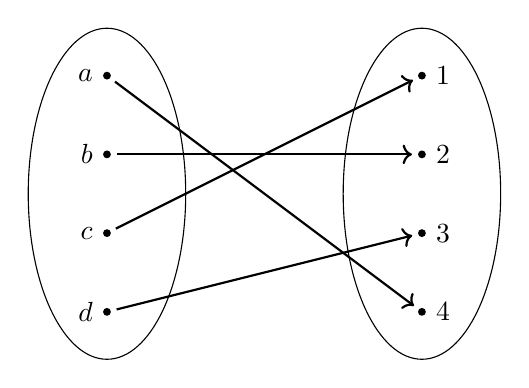
\begin{tikzpicture}[ele/.style={fill=black,circle,minimum width=.8pt,inner sep=1pt},every fit/.style={ellipse,draw,inner sep=-2pt}]
  \node[ele,label=left:$a$] (a1) at (0,4) {};    
  \node[ele,label=left:$b$] (a2) at (0,3) {};    
  \node[ele,label=left:$c$] (a3) at (0,2) {};
  \node[ele,label=left:$d$] (a4) at (0,1) {};

  \node[ele,,label=right:$1$] (b1) at (4,4) {};
  \node[ele,,label=right:$2$] (b2) at (4,3) {};
  \node[ele,,label=right:$3$] (b3) at (4,2) {};
  \node[ele,,label=right:$4$] (b4) at (4,1) {};

  \node[draw,fit= (a1) (a2) (a3) (a4),minimum width=2cm] {} ;
  \node[draw,fit= (b1) (b2) (b3) (b4),minimum width=2cm] {} ;  
  \draw[->,thick,shorten <=2pt,shorten >=2pt] (a1) -- (b4);
  \draw[->,thick,shorten <=2pt,shorten >=2] (a2) -- (b2);
  \draw[->,thick,shorten <=2pt,shorten >=2] (a3) -- (b1);
  \draw[->,thick,shorten <=2pt,shorten >=2] (a4) -- (b3);
 \end{tikzpicture}
\end{figure}
The two ovals are sets $A$ and $B$, and the dots inside the ovals are
their elements.  Hence $A$ consists of elements $a,b,c,d$, and $B$
consists of elements $1,2,3,4$.  We use the notation ``$a\in A$'' to
indicate that $a$ is an element of $A$.  (Thus, $\in$ is a binary
relation symbol, written in infix notation.)  The arrows from elements
in $A$ to elements in $B$ constitute a function $f:A\to B$, which
consists of an assignment of each element in $A$ to some element in
$B$.

The following axiomatization of set-theory prioritizes clarity over
rigor.  We have attempted to write the axioms in such a way that they
are easy to understand, but so that it's possible for the interested
reader to determine how they might be fully regimented in first-order
logic.

\begin{description}
\item[S1. Extensionality] The first axiom provides the condition under
  which two sets are equal, namely when they contain the same
  elements.
  \[ \forall A\forall B(A=B\lra \forall x(x\in A\lra x\in B)) . \]
  Similarly, two functions are equal if and only if they agree on all
  inputs.
  \[ \forall f\forall g(f=g\lra \forall x(f(x)=g(x)) .\]
\item[S2. Comprehension] The second axiom provides a method of
  building new sets from old sets.  It tells us that if we already
  have a set $A$, and if we can describe a property $\phi (x)$ of
  elements of $A$ (using the language of set theory), then there is a
  set $B$ of things that contain just those elements.  We sometimes
  write this set $B$ as $\{ x\in A \mid \phi (x) \}$, read as ``the
  $x$ in $A$ such that $\phi (x)$.''  The meaning of this axiom will
  be clearer after we see which sorts of properties $\phi (x)$ can be
  described in the language of set theory.
\item[S3. Empty Set]  The third axiom declares the existence of a set
  with no elements.
  \[ \exists A\forall x(x\not\in A) . \]
\end{description}
There will be a couple more axioms to come, but these first three will
suffice to prove some interesting basic facts about sets and
functions.  Consider the following claim and proof.

\begin{prop} There is only one empty set, that is $\exists !A\forall
  x(x\not\in A)$.  \end{prop}

\begin{proof} The empty set axiom says that there is at least one
  empty set; so we only need show that there is at most one.  Suppose
  then that $A$ and $B$ are empty sets.  That is,
  $\forall x(x\not\in A)$ and $\forall x(x\not\in B)$.  We will show
  first that $\forall x(x\in A\to x\in B)$.  Since
  $\forall x(x\not\in A)$, we have $a\not\in A$.  Hence by negative
  paradox, if $a\in A$ then $a\in B$.  Since $a$ was arbitrary,
  $\forall x(x\in A\to x\in B)$.  A similar argument shows that
  $\forall x(x\in B\to x\in A)$.  By extensionality, $A=B$.
\end{proof}

This proof is fully compliant with the inference rules you learned
earlier in this book.  You could, in fact, write it out in its full
glory, with dependency numbers, citations of rules, etc.  However,
it's slightly more pleasant for human beings to read and write proofs
with words.  Moreover, there's an art to saying just the right words
to convince your reader that the proof really does work.  One of the
goals of this section is to help you hone your skill as a writer of
clear and rigorous arguments.

It can be a lot easier to use set theory if we define some new
relation and function symbols.  We begin by using the fact we proved
above -- that there is a unique empty set -- to define a name
``$\emptyset$'' with the condition
\[ \forall A\bigl( A=\emptyset \: \lra \: \forall x(x\not\in A) \bigr)
  .\] We now define a binary relation symbol $\subseteq$ (written in
infix notation) that is intended to capture the idea of one set being
contained in another.
\begin{defn} For sets $A$ and $B$, we say that $A$ is a \textbf{subset} of $B$,
written $A\subseteq B$, just in case $\forall x(x\in A\to x\in B)$.
More formally,
\[ \forall A\forall B\bigl( A\subseteq B \: \lra \: \forall x(x\in
  A\to x\in B) \bigr) . \] \end{defn} Keep in mind that the
containment relation $\subseteq$ is very different than the
elementhood relation $\in$.  For most purposes in this book, you can
think of the elementhood relation $\in$ as standing between some $a$
that is {\it not} a set and a some $A$ that {\it is} a set.  For
example, you can think of yourself as an element or member of the set
of people who have read this sentence.  In contrast, the relation
$\subseteq$ can only hold between two sets.  Since you are not a set,
you cannot stand in the relation $\subseteq$ to anything
else.\footnote{For the advanced reader: we are intentionally
  maintaining a naive distinction between sets and non-sets.  If one
  really adopted ZF set theory as their ``theory of everything,'' then
  everything would be a set.}

We illustrate the definition of subset by showing that the emptyset
$\emptyset$ is a subset of every other set.

\begin{prop} $\forall B(\emptyset\subseteq B)$. \end{prop}

\begin{proof} Let $B$ be an arbitrary set.  Since
  $\forall x(x\not\in \emptyset )$, negative paradox gives
  $\forall x(x\in \emptyset\to x\in B)$.  By the definition of
  $\subseteq$, it follows that $\emptyset \subseteq B$.  Since $B$ was
  an arbitrary set, it follows that $\forall B(\emptyset\subseteq
  B)$. \end{proof}

\begin{exercises} Prove the following results.
  \begin{enumerate}
  \item $A\subseteq A$.  
  \item If $A\subseteq B$ and $B\subseteq C$ then $A\subseteq C$.
  \item If $A\subseteq B$ and $B\subseteq A$ then
    $A=B$. \end{enumerate} \end{exercises}

Recall that when a theory $T$ implies that a relation $\phi (x,y,z)$
is functional, then we may define a binary function symbol, say
$\cap$, by
\[ (x\cap y=z) \: \lra \: \phi (x,y,z) .\]
Consider then the following relation, definable in the theory of sets:
\[ \phi (A,B,C) \: \equiv \: \forall x(x\in C\lra (x\in A\wedge x\in
  B)) \] To see that $\phi$ is functional, suppose that $\phi (A,B,C)$
and $\phi (A,B,D)$.  A quick argument shows then that
$\forall x(x\in C\lra x\in D)$, and hence by extensionality, $C=D$.
Therefore, $\phi$ is functional, and we may define
\[ (A\cap B=C) \:\lra \: \phi (A,B,C)  .\]
In other words, 
\[ \forall x(x\in A\cap B\lra (x\in A\wedge x\in B)) . \] We call
$A\cap B$ the \emph{intersection} of $A$ and $B$.

\begin{exercises} Prove the following results. \begin{enumerate}
  \item $A\cap A=A$.
  \item $A\cap \emptyset = \emptyset$.
  \item $A\subseteq B$ if and only if $A\cap B=B$.
  \item $C\subseteq A\cap B$ if and only if $C\subseteq A$ and
    $C\subseteq B$.    
\end{enumerate} \end{exercises}

Similar to the definition of intersection, we can also define a \emph{union}
of sets.  Here the relevant relation is:
\[ \phi (A,B,C) \: \lra \: \forall x(x\in C\lra (x\in A\vee x\in B))
  . \] Since $\phi$ is functional, we may define a function symbol
$\cup$ with the feature
\[ \forall x(x\in A\cup B\lra (x\in A\vee x\in B)) . \]

\begin{exercises} Prove the following results.
  \begin{enumerate}
 \item $A\cup A=A$.   
 \item $A\cup \emptyset = A$.
 \item $A\subseteq B$ if and only if $A\cup B=B$.  
 \item $A\cap (B\cup C)=(A\cap B)\cup (A\cap C)$.
 \end{enumerate}
\end{exercises}

We need one more function on sets, namely the \emph{relative
  complement} of two sets.  The idea here is that $A\backslash B$
should consist of all those elements in $A$ that are {\it not} in $B$.
Thus, the defining condition is:
\[ \forall x(x\in A\backslash B\lra (x\in A\wedge x\not\in B)) . \] It
is frequently useful to speak as if a set $A$ has an absolute
complement $A^c$, i.e.\ the set of all things that are not in the set
$A$.  Mathematicians know that it's dangerous to talk about ``the set
of all things such that \dots '', but for many practical purposes we
can take some large set $X$ as the background domain, and then we can
think of $A^c$ as the relative complement of $A$ in $X$.

\begin{exercises} Let $A^c=X\backslash A$, and prove the
  following: \begin{enumerate}
  \item $(A\cup B)^c=A^c\cap B^c$.
  \item $(A\cap B)^c=A^c\cup B^c$.
  \item $A\cup A^c=X$.
  \item $A\cap A^c=X$.    
  \end{enumerate} \end{exercises}

The construction we perform now is not exactly a definition; in one
sense, it should be considered to be a new axiom.

\begin{description}
  \item[S4. Cartesian products] There is a construction process that takes two sets
$A,B$ as input, and that produces a new set $A\times B$ as output.
The set $A\times B$ is called the \emph{Cartesian product} of $A$ and
$B$. Each element of this new set $A\times B$ can be written in the
form $\langle a,b\rangle$ with the identity condition:
\[ \langle a,b\rangle = \langle c,d\rangle \: \lra \: a=c \wedge
  b=d . \] \end{description}

Note that the order in $\langle a,b\rangle$ matters; i.e.\ it is not
necessarily the case that $\langle a,b\rangle =\langle b,a\rangle$.
Accordingly, an element of the form $\langle a,b\rangle$ is called an
\emph{ordered pair}.

We define $\pi _1:A\times B\to A$ to be the function that takes each
ordered pair $\langle a,b\rangle$ to its first component $a$.
Similarly, we define $\pi _2:A\times B\to B$ to be the function that
takes each ordered pair $\langle a,b\rangle$ to its second component
$b$.

It's not difficult to see that if $A$ and $B$ are finite sets, then
the number $|A\times B|$ of elements in $A\times B$ is $|A|\cdot |B|$,
where $|A|$ is the number of elements in $A$, and $|B|$ is the number
of elements in $B$.  In fact, something like that result continues to
hold even when $A$ and $B$ are infinite.  However, that more general
result depends on developing a notion of different sizes of infinity,
and that's a subject for a more advanced book.

\begin{exercise} Show that if $A$ has $2$ elements and $B$ has $2$
  elements, then $A\times B$ has $4$ elements. \end{exercise}

\begin{exercise} Show that $\emptyset\times A=
  \emptyset$.  \end{exercise}

%% Show that powerset of A is in 1-to-1 correspondence with 2^A

Predicate logic makes heavy use of \emph{relation symbols}, such as
$Rxy$.  But what is a relation?  In the world of sets, we can think of
a \emph{relation} as a kind of set -- namely a subset of $A\times B$.
That might seem like a strange thing to say.  After all, if I asked
you to give me an example of a relation, you might suggest the
relation of being a parent, or the relation of being a sibling, or the
relation of being taller than.  In what sense are these relations like
a subset of $A\times B$?

Every relation has two aspects: an \emph{intension} and an
\emph{extension}.  The former, the intension, is a bit mysterious and
difficult to define, but basically it's supposed to be the essence or
meaning of the relation --- what makes it the particular relation that
it is.  The latter, the extension, is easier to define: the extension
of a relation is just the set of ordered pairs that stand in that
relation.  So, for example, the extension of the relation ``has been
married to'' consists of all pairs of people who have been married to
each other, including
\[ \langle\text{Donald},\text{Marla}\rangle , \quad
  \langle\text{Donald},\text{Ivana}\rangle , \quad
  \langle\text{Donald},\text{Melania}\rangle . \] So far we've just
been taking about binary relations, i.e.\ those that hold between two
things.  There are, however, $n$-ary relations for every natural
number $n$.  The unary relations more frequently go under the name of
\emph{properties}.  Just like other relations, a property has an
intension and an extension.  Thus, the extension of a property is
simply the set of those things that possess the property.

Interestingly, properties with distinct intension can have the same
extension.  A famous example used by W.v.O. Quine are the properties
``$x$ is a living creature with a heart'' and ``$x$ is a living
creature with kidneys''.\footnote{See Quine, ``Two dogmas of
  empiricism'' {\it The Philosophical Review} 60, 20--43 (1951)}
Obviously, having a heart is not the same thing as having kidneys.
However, any living creature has a heart if and only if it has
kidneys.  Therefore, these two properties have the same extension.

It's surprisingly useful to classify relations into different kinds.
Here we'll talk about two special kinds of relations: equivalence
relations and functional relations.

\subsection{Equivalence relations}

We frequently have several names for the same thing.  If $a$ and $b$
are names for the same thing, then we would say ``$a$ is identical to
$b$'', or in short ``$a=b$''.  As we saw before, the equality relation
has a peculiar logic.  For example, we take it for granted that $a=a$
(which is certainly not the case for every relation).  We also showed
that if $a=b$ then $b=a$; and that if $a=b$ and $b=c$, then $a=c$.
While the equality relation has these features, it's not the only
relation with them.  For example, consider the relation $R$ where
$\langle a,b\rangle\in R$ just in case $a$ is the same height as $b$.
Then $\langle a,a\rangle \in R$ (i.e.\ everyone is the same height as
themselves); if $\langle a,b\rangle\in R$ then
$\langle b,a\rangle\in R$ (being the same height as is symmetric); and
if $\langle a,b\rangle\in R$ and $\langle b,c\rangle\in R$ then
$\langle a,c\rangle\in R$ (being the same height as is
transitive). These facts show that $R$ is an equivalence relation.

A relation $R$ on $A\times A$ is said to be an \emph{equivalence
  relation} just in case it is:
\begin{description}
\item[reflexive] For all $a\in A$, $\langle a,a\rangle\in R$.
\item[symmetric] For all $a,b\in A$, if $\langle a,b\rangle\in R$ then
  $\langle b,a\rangle\in R$.
\item[transitive] For all $a,b,c\in A$, if $\langle a,b\rangle\in R$
  and $\langle b,c\rangle\in R$ then $\langle a,c\rangle\in R$.
\end{description}
The simplest example of an equivalence relation is the equality
relation $R=\{ \langle a,a\rangle \mid a\in A\}$. Another equivalence
relation is the relation of having the same value for a certain
quantity.  For example, ``$x$ is the same height as $y$'' is an
equivalence relation on the set of people.

\begin{exercises} \mbox{} \begin{enumerate} \item Let $R$ be an equivalence relation, and let $[a]$ be
  the set of all things related to $a$, that is
  \[ [a] \: = \: \{ b \mid \langle a,b\rangle\in R\} . \]
  Show that either $[a]=[b]$ or $[a]\cap [b]=\emptyset$.
\item Suppose that $R$ and $S$ are equivalence relations.  Show that
  $R\cap S$ is an equivalence relation.
\item Let $\phi\equiv\psi$ be the inter-derivability relation in
  propositional logic.  Show that $\equiv$ is an equivalence
  relation. \end{enumerate} \end{exercises}


\subsection{Functional relations}

There are several different ways to think of what a \emph{function}
is.  First, a function can be thought of as a {\it rule} that assigns
elements of one set to elements of another set.  Second, a function
can be conceived of as a {\it graph}, i.e.\ a set of ordered pairs in
a plane.  You might remember that for a graph to be a function it has
to have the feature that any vertical line intersects it in only one
point.  In other words, the graph of a function has the feature that
if both $\langle a,b\rangle$ and $\langle a,c\rangle$ occur in the
graph, then $b=c$.

\begin{figure}[h] \centering
\begin{tikzpicture}
      \draw[->] (-3,0) -- (3,0) node[right] {$x$};
      \draw[->] (0,-2) -- (0,3) node[above] {$y$};
      \draw[scale=0.5,domain=-2.5:2.5,smooth,variable=\x,black] plot
      ({\x},{\x*\x});
    \end{tikzpicture}
\caption{Graph of the function $f(x)=x^2$.  The parabola is the set
  of ordered pairs $\langle x,x^2\rangle$.}    
\end{figure}

Many familiar functions are not really functions in the strict sense.
Consider, for example, the inverse function $\frac{1}{x}$.  This
operation isn't defined at $0$, and so it isn't really a function on
all real numbers (i.e.\ its domain set is not the set of all real
numbers).  We require that a function is defined on all elements of
its domain set, that is, for all $x$ in the domain, there is an $f(x)$
in the codomain.

A relation $R$ on $A\times B$ is said to be a \emph{functional
  relation} just in case it satisfies:
\begin{description}
\item[existence] For all $a\in A$ there is a $b\in B$ such that
  $\langle a,b\rangle\in R$.
\item[uniqueness] If $\langle a,b\rangle \in R$ and $\langle
  a,c\rangle\in R$ then $b=c$.
\end{description}
Any function $f:A\to B$ gives rise to a functional relation called its
graph: 
\[ \mathrm{graph}(f) \: = \: \{ \langle x,f(x)\rangle \mid x\in X
  \} \] By the extensionality axiom, there is a one-to-one
correspondence between functions and functional relations, i.e.\ each
function corresponds to precisely one functional relation, and if two
functions are distinct, then they correspond to distinct relations.

Since functions are relations, functions have both an intension and an
extension.  You may already have observed that fact, i.e.\ that a
single function can be expressed in various ways.  Consider, for
example, the functions:
\[ f(x)=x^2-1 ,\qquad g(x)=(x+1)(x-1) .\] Here we might say that $f$
and $g$ have different intensions, since they provide different
recipes for calculating an output.  Nonetheless, these two recipes
always produce the same output, hence $f$ and $g$ have the same
extension.

Functions, like relations, have an \emph{arity}, i.e.\ a number of
inputs.  Unlike relations, however, functions always have a single
output.  A function like $f(x)=x^2-1$ is unary, i.e.\ it takes one
input.  In contrast, the addition function is binary, i.e.\ its input
is two numbers.  In the limiting case, a $0$-ary function has no
inputs, and one output.  Such a function is called a \emph{point} or
an \emph{element}, i.e.\ it is an element in a set.

Since points are a special case of functions, which is a special case
of a relation, it also follows that a point has both an intension and
an extension.  To see what's going on here, it may be easier to think
of a point as a name.  Then the intension of a name is its
connotation, and the extension of a name is its
denotation.\footnote{For further investigation of this issue, see
  Gottlob Frege's discussion of ``morning star'' and ``evening
  star.''}

If $f$ is a function from $A$ to $B$, and $g$ is a function from $B$
to $C$, then we may define a function $g\circ f$ from $A$ to $C$ by
setting
\[ (g\circ f)(x) \: = \: g(f(x)),\qquad \forall x\in A .\]

\begin{exercise} Show the rather trivial fact that
  $h\circ (g\circ f)=(h\circ g)\circ f$, whenever $f,g$ and $h$ have
  domains and codomains that align in the right way. \end{exercise}

\begin{exercise} Suppose that $R=\mathrm{graph}(f)$ and
  $S=\mathrm{graph}(g)$.  Show that
  \[ \mathrm{graph}(g\circ f)\: = \: \bigl\{ \langle x,z\rangle \mid
    \exists y(\langle x,y\rangle \in R\wedge \langle y,z\rangle\in S) \bigr\} .\]  \end{exercise}

% \begin{figure}[h] \label{many}
%  \centering
%  \begin{tikzpicture}[ele/.style={fill=black,circle,minimum width=.8pt,inner sep=1pt},every fit/.style={ellipse,draw,inner sep=-2pt}]
%   \node[ele,label=left:$a$] (a1) at (0,4) {};    
%   \node[ele,label=left:$b$] (a2) at (0,3) {};    
%   \node[ele,label=left:$c$] (a3) at (0,2) {};
%   \node[ele,label=left:$d$] (a4) at (0,1) {};

%   \node[ele,,label=right:$1$] (b1) at (4,4) {};
%   \node[ele,,label=right:$2$] (b2) at (4,3) {};
%   \node[ele,,label=right:$3$] (b3) at (4,2) {};
%   \node[ele,,label=right:$4$] (b4) at (4,1) {};

%   \node[draw,fit= (a1) (a2) (a3) (a4),minimum width=2cm] {} ;
%   \node[draw,fit= (b1) (b2) (b3) (b4),minimum width=2cm] {} ;  
%   \draw[->,thick,shorten <=2pt,shorten >=2pt] (a1) -- (b4);
%   \draw[->,thick,shorten <=2pt,shorten >=2] (a2) -- (b1);
%   \draw[->,thick,shorten <=2pt,shorten >=2] (a3) -- (b1);
%   \draw[->,thick,shorten <=2pt,shorten >=2] (a4) -- (b3);
% \end{tikzpicture}
% \label{many} \caption{A function that is neither one-to-one, nor onto}
% \end{figure}

\begin{exercises} \mbox{} \begin{enumerate}
\item Consider the function $f(x)=x^3$ on real numbers.  Is
  $f$ one-to-one?  Is $f$ onto?
\item Give an example of a functional relation that can be described
  in the vocabulary of a typical ten year old child.
\item Show that if $g\circ f$ is one-to-one, then $f$ is one-to-one.
\item Give an example of functions $g$ and $f$ where $g\circ f$ is
  one-to-one, but $g$ is not one-to-one.  
\end{enumerate} \end{exercises}

%% will this next little bit be useful?  Why do it?

Given a function $f:X\to Y$, there's a natural way to define a couple
of other functions.  First of all, we define an \emph{inverse image}
function $f^{-1}$ that maps subsets of $Y$ to subsets of $X$.  In
particular, 
\[ (x\in f^{-1}(A)) \: \lra \: (f(x)\in A) . \]
In other words,
\[ f^{-1}(A) \: = \: \{ x\in X \mid f(x)\in A \} .\] The set
$f^{-1}(A)$ is called the \emph{inverse image} or \emph{preimage} of
$A$ under $f$.  We now show that inverse image preserves intersections.

\begin{prop} $f^{-1}(A\cap B)=f^{-1}(A)\cap f^{-1}(B)$.
\end{prop}

\begin{proof} We string together a series of biconditionals.
  \[ \begin{array}{l l l}
       x\in f^{-1}(A\cap B) & \lra & f(x)\in A\cap B \\
                            & \lra & f(x)\in A\wedge f(x)\in B \\
                            & \lra & x\in f^{-1}(A)\wedge x\in f^{-1}(B) \\
       & \lra & x\in f^{-1}(A)\cap
                f^{-1}(B) . \end{array} \] \end{proof}

Whereas the preimage mapping $f^{-1}$ takes subsets of $Y$ to subsets
of $X$, the \emph{image} mapping moves in the opposite direction.  Here we
abuse notation by using $f$ again for the image mapping which applies
to subsets of $X$, instead of to elements of $X$.  We define
\[ f(A) \: = \: \{ y\in Y \mid \exists x(x\in A\wedge f(x)=y) \} . \]
That is, $f(A)$ consists of those elements in $Y$ that are in the
range of $A$ under the mapping $f$.  In general, it is not the case
that $f(A\cap B)=f(A)\cap f(B)$.  Suppose, for example, that
$A\cap B=\emptyset$, and that $f$ is a function such that
$f(A)=f(B)=Y$.  Then $f(A\cap B)=f(\emptyset )=\emptyset$, but
$f(A)\cap f(B)=Y$.

\begin{exercises} Prove the following for arbitrary sets $A,B$, and
  function $f:A\to B$.
   \begin{enumerate}
   \item $f^{-1}(A\cup B)=f^{-1}(A)\cup f^{-1}(B)$.  
   \item If $A\subseteq B$ then $f^{-1}(A)\subseteq f^{-1}(B)$.
   \item $f(A\cup B)=f(A)\cup f(B)$.
   \item If $f$ is a one-to-one function, then $f(A\cap B)=f(A)\cap f(B)$.
   \end{enumerate}
 \end{exercises}

%% TO DO: move the following? 
\begin{exercise} Show that if $f:A\to B$ is one-to-one, and $A$ is
  non-empty, then there is a function $g:B\to A$ such that $g\circ f$
  is the identity function on $A$. \end{exercise}
 
Axioms S1--S4 tell us what sets must be like, but they don't say much
about which sets exist, other than the empty set.  Our next axiom
ensures us of the existence of a set whose elements form an infinite
progression.  You know this set under the common description:
$0,1,2,\dots $, i.e.\ the \emph{natural numbers} $N$.  The key
property of $N$ is that has an origin $0$, and a successor function
$s(x)=x+1$ that enumerates all its elements.
\begin{description}  
\item[S5. Infinity] There is a set $N$, with element $0\in N$, and a
  function $s:N\to N$ such that: $s$ is one-to-one, but not onto, and
  every element of $N$ can be reached by a finite number of
  applications of $s$ to $0$. \end{description} Successive
applications of $s$ allow us to name all of the elements in $N$:
\[ 1=s(0),2=s(s(0)),\dots .\] We can then use the comprehension axiom
to define all the finite and co-finite subsets of $N$, such as
\[ \{ x\in N \mid x=2\vee x=4 \} ,\qquad \{ x\in N \mid x\neq 3 \} .\]
It follows then that for each natural number $n$, there is a set $S_n$
with exactly $n$ elements.  As a convenient shorthand, we will write
$\{ a_1,\dots ,a_n\}$ for the set
\[ \{ x\in N \mid x=a_1\vee\cdots \vee x=a_2 \} .\] Then
extensionality entails that duplicate items can be removed from a set,
for example $\{ a,a,b \}=\{ a,b\}$.

The structure of the natural numbers $N$ makes it possible to define
an addition function $+$ and a multiplication function $\cdot$.  For
example, we set $x+0=x$, and $x+s(y)=s(x+y)$.  It can be shown that
$+,\cdot ,0,1$ satisfy the Peano axioms for arithmetic.  Thus, there
is a clear sense in which the theory PA can be translated into the
theory of sets.  This translation provides the desired reduction of at
least one important part of mathematics, viz.\ arithmetic, to set
theory.

For the comprehension axiom, one might think it would be simpler just
to say that for any formula $\phi (x)$, there is a set $\{ x | \phi
(x) \}$ of all things that satisfy $x$.  But that idea leads
immediately to problems, as was noted by Bertrand Russell.  Consider,
for example the following predicate:
\[ \phi (x)\: \equiv \: x\not\in x , \] and let
$A=\{ x\mid \phi (x)\}$.  In other words, $A$ is the set of all sets
that do not contain themselves.  

\begin{exercise} Show that if $A\in A$ then $A\not\in A$.  Then show
  that if $A\not\in A$ then $A\in A$.  Conclude that the assumption
  that $A$ exists leads to a contradiction. \end{exercise}

It turns out then not to be so easy to formulate a theory of sets that
is both \emph{consistent}, and that is powerful enough to serve as a
foundation for mathematics.


%%% Local Variables:
%%% mode: latex
%%% TeX-master: "main"
%%% End:


\chapter{Models} \label{inter}

The primary goal of this chapter is to teach you how to {\it prove}
that an argument is invalid.  The idea here is like truth-tables, but
the method more closely resembles what one actually does in real-life
scenarios, especially in the sciences.

A typical (scientific) theory is applicable in many different
situations.  For example, Darwin's theory of evolution applies to
early human history, but it also applies to populations of
fruit-flies, or to cancer cells.  Similarly, a theory about economic
bubbles might apply to the housing bubble in the US in the early
2000s, and also to the tulip crisis of 1637 in Holland.  So,
scientific thinking involves both abstract theory, and the application
of that theory to specific situations --- or, to be more precise,
application to more concrete descriptions of situations.  We'll say
that the concrete description is a \emph{model} of the abstract
theory.\footnote{Warning: the English verb ``to model'' is used in two
  almost opposite ways.  First, one can model a concrete thing by
  constructing an abstract representation of it.  Second, one can
  model an abstract idea or theory by constructing a more concrete
  instance of it.  In this chapter, we will be concerned exclusively
  with the second sense of modelling.}

For our purposes, the primary utility of model-building is that we can
use it to show that an argument is invalid.  For, if one can build a
model where the premises of an argument are true, but its conclusion
is false, then that argument is invalid.  What then are the rules for
model-building, and how can we tell whether or not sentences are true
in a model?  To get answers to these questions, let's begin with a
famous example where model-building played a crucial role.

For most of western history, Euclidean geometry was taken to be the
paradigm example of certain knowledge.  Sitting in a dark room, you
can use Euclidean geometry to deduce, with complete logical rigor,
that in any triangle, the sum of the internal angles is $180$ degrees.
Then if you go outside and measure triangles, you will find again and
again that the prediction of Euclidean geometry is correct: the
internal angles always add up to $180$ degrees.

It seems almost like a miracle that Euclidean geometry --- discovered
more than two thousand years ago --- could be so certain.  This kind
of thought led many people throughout history to investigate the
source of our knowledge of the axioms of Euclidean geometry.  Some of
these investigations were of a philosophical nature, and others were
focused on mathematical questions, such as: is it possible to boil
down the number of axioms of Euclidean geometry so that we're left
with just a few axioms that are obviously true?

We won't go into details here, but just think about it this way.  Some
of the axioms of Euclidean geometry seem to be self-evidently true.
For example, between any two points, there is a line; or similarly,
any two right angles are equal to each other.  Let's write $\Gamma$
for the collection of these uncontroversial axioms.

However, Euclidean geometry also depends on the following, less
obvious, axiom:
\begin{quote}
  Parallel postulate: for any line $x$, and for an point $p$ not on
  $x$, there is a unique line $y$ such that $p\in y$ and such that $y$
  is parallel to $x$. \end{quote} Let's write $P$ for the parallel
postulate.  Because $P$ is not obviously true on its face, many
mathematicians spent a lot of time trying to prove that it follows
from the uncontroversial axioms.  That is, they tried to show that
$\Gamma\vdash P$.  I'm sorry to say that some of these mathematicians
spent their whole lives trying to prove this little sequent, and died
without having found an answer.  In fact, nobody ever managed to prove
it.

\label{loba}

But then something amazing happened.  In the nineteenth century, an
obscure Russian mathematician named Nikolai Lobachevsky decided that
he would try for a proof.  Being a clever logician, Lobachevsky
realized that all he had to do was to prove that $\Gamma$ and $\neg P$
imply a contradiction.  So, he assumed the uncontroversial axioms and
the {\it negation} of the parallel postulate, and he got busy working
his way toward a contradiction.  Lobachevsky proved many things that
seemed absurd.  For example, he proved that the internal angles of a
triangle are strictly less than $180$ degrees.  However, he never got
a literal contradiction, i.e.\ he never got a sentence $\phi$ and also
its negation $\neg \phi$.

After a while, it dawned on Lobachevsky that he had proven so many
things that these consequences amounted to the description of a new
mathematical universe.  In other words, he had described a model $M$
in which the uncontroversial axioms $\Gamma$ are true, and the
parallel postulate $P$ is false.  This model $M$ is a non-euclidean
universe, which means that our universe isn't necessarily Euclidean.
Therefore, the method of modelling is responsible for history's most
famous example of showing that we don't know something that we thought
we knew.

\section{Logical grammar}

The intuitive ideas of interpretations and models are really
interesting and suggestive.  These ideas have proven to be extremely
useful in many domains of knowledge, from mathematics to economics and
philosophy.  However, as we've described them so far, these ideas are
too vague to {\it prove} anything interesting about them, and a
fortiori, to use them to prove anything about the system of logic
we've developed in this book.

The tool we develop here is the notion of an \emph{interpretation} of
a predicate logic language into the theory of sets.  For this we
assume that that we have a fairly firm grasp of what is true or false
in the universe of sets.  Thus, in order to show that a sequent
$\phi\vdash\psi$ is not valid, we will show that $\phi$ and $\psi$ can
be interpreted as set-theoretic statements such that $\phi$ is
obviously true, and $\psi$ is obviously false.

To this end, we first need a precise description of the family of
predicate logic sentences.  Suppose that $\Sigma$ is a fixed predicate
logic signature.  That is, $\Sigma$ consists of function symbols and
relation symbols.  We'll also assume that $\Sigma$ comes with an
equality symbol.  We then define the set of $\Sigma$-\emph{terms} as
follows:
\begin{itemize}
\item Each variable $x,y,z,\dots $ is a $\Sigma$-term.
\item If $f\in\Sigma$ is an $n$-ary function symbol, and
  $t_1,\dots ,t_n$ are $\Sigma$-terms, then $f(t_1,\dots ,t_n)$ is a
  $\Sigma$-term.
\end{itemize}
When no confusion can result, we'll just say ``term'' instead of
``$\Sigma$-term''.  The special case of a $0$-ary function symbol is
called a \emph{name} or a \emph{constant symbol}.

This definition of terms should agree with the intuitions you have
already developed.  For example, if $\Sigma$ comes with a binary
function symbol $\circ$, then the terms include expressions such as
$x\circ y$ and $(x\circ y)\circ z$.  If $\Sigma$ comes with a name $1$
and a binary function symbol $+$, then the terms include expressions
such as $1+1$ and $(1+1)+(1+1)$.  Semantically speaking, the terms
will be interpreted as functions; and in the special case of names,
will be interpreted as points.

We define the set of $\Sigma$-\emph{formulas} as follows:
\begin{itemize}
\item If $t_1$ and $t_2$ are terms, then $t_1=t_2$ is a formula.
\item If $R$ is an $n$-ary relation symbol and $t_1,\dots ,t_n$ are
  terms, then $R(t_1,\dots ,t_n)$ is a formula.
\item If $\phi$ and $\psi$ are formulas, then $\phi\vee\psi$,
  $\phi\wedge\psi$, $\phi\to\psi$ and $\neg\phi$ are formulas.
\item If $\phi$ is a formula that does not contain the quantifiers
  $\forall x$ or $\exists x$, then $\forall x\phi$ and $\exists x\phi$
  are formulas.
\end{itemize}
A few comments on this definition of formulas.  First, to be more
rigorous, we might want to define simultaneously the notion of a
formula and the notion of the variables that occur freely in that
formula.  However, we will operate for now on a more intuitive level.
Basically, a variable occurs \emph{freely} in a formula if that
variable hasn't at any stage of construction been bound by a
quantifier.  So, for example, in the formula $x=y$, the variables $x$
and $y$ both occur freely.  However, in the formula $\forall x(x=y)$,
the variable $x$ has been bound, and only $y$ occurs freely.

Second, the quantifier clause of our definition is clumsy.  It would
be simpler to allow formulas like $\forall x(Px\to \exists xQx)$, but
that is not permitted by our quantifier clause.  The reason for the
more restrictive clause is simply to encourage the student to use
perspicious notation.  While there is no reason in theory to ban
sentences such as $\forall x(Px\to \exists xQx)$, it's better to use a
variant such as $\forall x(Px\to \exists yQy)$ in which it's clear
that the first quantifier applies only to the first occurence of $x$.

We now define a predicate logic \emph{sentence} to be a formula in
which no variables are free.  Thus, $\exists xRax$ is a sentence, but
$\exists xRyx$ is not a sentence since $y$ is free.  Our proofs will
always and only involve sentences.  If you ever have a step in a proof
that has a formula rather than a sentence, then you've misapplied one
of the inference rules.\footnote{The most elegant proof systems allow
  sequents with free variables.  But baby steps
  \dots }


\section{Interpretation formalized}

An \emph{\gls{interpretation}} of the symbols in $\Sigma$ consists of
four things:
\begin{enumerate}
\item Some fixed set $M$, which we call the \emph{domain} or
  \emph{universe} of the interpretation.  For technical reasons, the
  domain $M$ must be a nonempty set.\footnote{This requirement has
    bothered many logicians, including Bertrand Russell.  It can be
    avoided by using an alternative to classical logic such as free
    logic or coherent logic.}
\item An assignment of each $n$-ary relation symbol $R\in\Sigma$ to
  some subset $R^M$ of $M\times\cdots\times M$.  The set $R^M$ is
  called the \emph{extension} of $R$ in $M$.
\item An assignment of each constant symbol $c\in\Sigma$ to some
  element $c^M\in M$.
\item An assignment of each $n$-ary function symbol $f\in\Sigma$ to
  some function $f^M$ from $M\times\cdots\times M$ to $M$.
\end{enumerate}
There will always be many different ways that the symbols in $\Sigma$
could be interpreted.  There is so much freedom here it can be
dizzying.  How should one choose the set $M$ from among the untold
number of conceivable sets?  Fortunately, it doesn't make any
difference which particular set you choose.  All that matters are
structural facts, namely, the size of the set, the size of the
extensions of the relation symbols, and the relations between the
extensions of the relation symbols.  For many cases, you'll be able to
tell whether a sentence is consistent or inconsistent by looking at
interpretations in finite sets.  For some sentences, you'll need an
infinite set, e.g.\ the natural numbers.  For the exercises in this
book, you'll never need a set bigger than the natural numbers.

Once the symbols in $\Sigma$ have been assigned to relevant
set-theoretic items, there is a straightforward recipe for extending
the assignment to all terms and formulas built on $\Sigma$.  As with
valuations (i.e.\ rows in truth tables), the assignment grows, from
the inside out, starting with the assignments to the function and
relation symbols, and then applying set-theoretic operations
corresponding to the connectives and quantifiers.

Let's begin by looking at the case of a formula $\phi (x)$ in which
only the variable $x$ occurs.  In this case, we'll define
$\phi (x) ^M$ to be a subset of $M$, which can be thought of as
follows:
\begin{quote} $\phi (x)^M$ is the set of all $a\in M$ such that
  $\phi (x)$ is true when $x$ takes value~$a$.  \end{quote} The
definition of $\phi (x)^M$ is inductive.  In particular, we first
define $\phi (x)^M$ when $\phi (x)$ is an atomic formula.  Then we
extend the definition to complex formulas.  

If we temporarily ignore function symbols, then an atomic formulas
that contains only the variable $x$ is either of the form $x=x$, or of
the form $R(x,\dots ,x)$.
\begin{itemize}
  \item Since $(x=x)^M$ should be the set of all
    $M$ that are equal to themselves, it should be all of $M$.
  \item As for $R(x,\dots ,x)^M$, since $R^M$ is defined to be a subset of
$M\times\cdots \times M$, we can define $R(x,\dots ,x)^M$ to be the
set of all $a\in M$ such that $\langle a,\dots ,a\rangle\in R^M$.
More formally, 
\[ R(x,\dots ,x)^M \: = \: \{ a\in M \mid \langle a,\dots ,a\rangle
  \in R^M \} .\]
\end{itemize}
Now that we have a definition of $\phi (x)^M$ for an atomic formula
$\phi (x)$, we extend the definition to Boolean combinations of
formulas.  In particular,
\[ \begin{array}{r c l p{0.2cm} r c l}
     (\phi\wedge\psi )^M &=& \phi ^M\cap \psi ^M  & & (\phi\vee\psi
                                                      )^M & = & \phi
                                                                ^M\cup
                                                                \psi
                                                                ^M \\ \\
     (\neg\phi )^M &=&  M\backslash \phi ^M & & (\phi\to\psi )^M &=& 
                                             (M\backslash \phi ^M)\cup
                                             \psi ^M \end{array} \]
These definitions are fairly intuitive.  For example, $(\phi\wedge
\psi )^M$ is true of some $a$ just in case both $\phi ^M$ and $\psi^M$
are true of $a$.  For the case of $\phi\to\psi$, we use the intuitive
equivalence with $\neg\phi\vee\psi$ and the previous definitions.

Finally, we need to extend the interpretation to formulas that are
built up with quantifiers --- and here we run into a little challenge.
If $\phi (x)$ has a free variable $x$, then $\exists x\phi (x)$ no
longer has a free variable, and so it doesn't make much sense to think
of $\forall x\phi (x)$ as a set of things.  Instead, we want to think
of $\forall x\phi (x)$ as simply being true or false.  The obvious
thing to say here is that $(\exists x\phi (x))^M$ is true when
$\phi (x)^M\neq\emptyset$, and $(\exists x\phi (x))^M$ is false when
$\phi (x)^M=\emptyset$.  Similarly, $(\forall x\phi (x))^M$ is true
when $\phi (x)^M=M$, and $(\forall x\phi (x))^M$ is false when
$\phi (x)^M\neq M$.

\begin{example} Suppose that $F$ and $G$ are predicate symbols.  Let
  $M=\{ 1,2,3\}$, let $F^M=\{ 1,2\}$, and let $G=\{ 2,3\}$.  We can
  then compute
\[ \begin{array}{c c l c l} (Fx\wedge Gx)^M & = & (Fx)^M\cap (Gx)^M
     & = & \{ 2\}   \\
     (Fx\vee Gx)^M & = & (Fx)^M\cup (Gx)^M & = & M \\
     \exists x(Fx\wedge Gx)^M & = & \mathsf{true} \\
   \forall x(Fx\wedge Gx)^M & = &
                                  \mathsf{false}  \end{array} \]  \end{example}

\begin{example} Consider the sentence $Fc$.  Let $M$ be an
  interpretation with domain $\{ 1,2\}$ where $F^M=\{ 1\}$ and
  $c^M=2$.  Then $Fc$ is false in $M$.  Let $N$ be an interpretation
  just like $M$ except that $c^N=1$.  Then $Fc$ is true in
  $N$. \end{example}
                            
There are two primary reasons to build interpretations: to show that a
collection of sentences is consistent, and derivatively, to show that
a sequent cannot be proven.  In propositional logic, a sentence $\phi$
is consistent just in case there is some valuation $v$ such that
$v(\phi )=1$.  In predicate logic, a sentence $\phi$ is consistent
just in case there is some interpretation $M$ such $\phi ^M$ is true.
In propositional logic, a sequent $\phi\vdash\psi$ is provable if and
only if every valuation that makes $\phi$ true also makes $\psi$ true.
In predicate logic, a sequent $\phi\vdash\psi$ is provable if and only
if for any interpretation $M$, if $\phi ^M$ is true then $\psi ^M$ is
true.  To show, then, that a sequent cannot be proven, it suffices to
produce an interpretation that makes its premises true and its
conclusion false.

\begin{defn} A \emph{\gls{counterexample}} to a sequent
  $\phi\vdash\psi$ is an interpretation $M$ such that $\phi ^M$ is
  true, but $\psi ^M$ is false. \end{defn}

A counterexample is a concrete illustration of the failure of an
argument to preserve truth.  That is, a counterexample to an argument
is a formalization of the notion of a situation, or state of affairs,
in which the premises are true and the conclusion is false.

\begin{example} It is intuitively clear that $\forall x(Fx\vee Gx)$
  doesn't imply $\forall xFx\vee \forall xGx$.  We'll now construct a
  formal counterexample.  Let $M=\{ 1,2\}$, let $F^M=\{ 1\}$, and let
  $G^M=\{ 2\}$.  Then
  \[ (Fx\vee Gx)^M \:=\: (Fx)^M\cup (Gx)^M \: =\: \{1\}\cup \{ 2\}
    \:=\: M , \] hence $(\forall x(Fx\vee Gx))^M$ is true.  Since
  $2\not\in F^M$, it follows that $(\forall xFx)^M$ is false.
  Similarly, $(\forall xGx)^M$ is false, and hence
  $(\forall xFx\vee \forall xGx)^M$ is false.  Therefore, $M$ shows
  that $\forall x(Fx\vee Gx)$ does not imply
  $\forall xFx\vee\forall xGx$. \end{example}

You might wonder: how did we know to choose this interpretation?
Well, I'm sorry to say that there is no algorithm for finding
predicate logic interpretations.\footnote{The technical claim here is
  that predicate logic is \emph{undecidable}.}  In this way, predicate
logic differs markedly from propositional logic, where the truth-table
method provides a sure-fire method for finding the interpretation you
want.  Nonetheless, with practice, a human being can become quite good
at sniffing out the relevant interpretations.  For example, can I
think of a situation where everything is $F$ of $G$, but it's not true
that everything is $F$, and it's not true that everything is $G$?
What immediately comes to my mind here, as a counterexample, is even
and odd numbers.  Every number is either even or odd; but it's not
true that every number is even, and it's not true that every number is
odd.  So, I could have chosen domain $M=\{ 1,2,\dots \}$, and let
$F^M$ be odd numbers and $G^M$ be even numbers.  But then I realized
that two numbers were enough to show that the argument is invalid, and
that's why I chose $M=\{ 1,2\}$ with $F^M=\{ 1\}$ and $G^M=\{ 2\}$.

There's another approach that is sometimes helpful, but it's not
guaranteed to succeed.  In particular, you can start to get a feel for
whether or not an argument is valid by looking at what it says about
small domains.  For example, if you take a domain $M=\{ a,b\}$ with
two elements, then an existential sentence $\exists x\phi (x)$ says
that \mbox{$\phi (a)\vee \phi (b)$}, and a universal sentence
$\forall x\psi (x)$ says that $\psi (a)\wedge\psi (b)$.  In some
cases, you'll get lucky by looking at small domains, and you'll be
able to see directly how to build a counterexample.  In the example
above, $\forall x(Fx\vee Gx)$ says that
$(Fa\vee Ga)\wedge (Fb\vee Gb)$, and $\forall xFx\vee\forall xGx$ says
that $(Fa\wedge Ga)\vee (Fb\wedge Gb)$.  Then a simple truth-table
test shows that the valuation $v(Fa)=v(Gb)=1$ and $v(Ga)=v(Fb)=0$
makes the first sentence true and the second sentence false.  From
this, we see that $F^M=\{ a\}$ and $G^M=\{ b\}$ gives a counterexample
to the argument.\footnote{There is, in fact, an algorithm for
  determining the validity of arguments that use only unary predicate
  symbols. See p.\ \pageref{algorithms}.}
                              
\begin{exercises} 
  For each of the following sequents, provide a counterexample to show
  that it is invalid.
  \begin{enumerate}
  \item $\exists xFx\:\vdash \: Fc$
  \item $Fc\:\vdash \: \forall xFx$    
\item $\exists xFx\wedge\exists xGx\:\vdash\:\exists x(Fx\wedge Gx)$
\item $\forall xFx\to\forall xGx\:\vdash\:\forall x(Fx\to Gx)$
\item $\forall x(Fx\to Hx) \:\vdash\:\exists xFx\vee \neg
  \exists xHx$
\item $\forall x(Fx\to Gx)\:\vdash\:\exists x(Fx\wedge Gx)$
\item $\exists x(Fx\wedge Gx),\exists x(Gx\wedge Hx)\:\vdash\:\exists
  x(Fx\wedge Hx)$
\item $\vdash\:\forall xFx\vee \forall x\neg Fx$
\item $\exists x(Fx\to Gx),\exists x(Gx\to Hx)\:\vdash\:\exists
  x(Fx\to Hx)$
\item $\exists x(Fx\to Gx)\:\vdash\: \exists xFx\to \exists xGx$
\end{enumerate} \end{exercises}

\begin{exercise} Suppose that $\phi$ and $\psi$ are formulas where
   the only free variable is $x$.  Show that $(\phi\to \psi)^M=M$ iff
   $\phi ^M\subseteq \psi^M$.
 \end{exercise}

Let's now expand the definition of an interpretation to cover
propositional constants as well.  An interpretation assigns a propositional constant a truth value,
either true ($1$) or false ($0$).  But now we have to think about how
to extend an interpretation to formulas that contain both predicate
symbols and propositional constants.  Here we adopt the following
definitions:
\[ \begin{array}{r c l c | c r c l}
     \multicolumn{3}{c}{\text{$P^M$ is false}} & & & \multicolumn{3}{c}{\text{$P^M$ is true}} \\
     \hline
     (\phi \wedge P)^M &= & \emptyset & & &  (\phi \wedge P)^M &=& \phi
                                   ^M  \\
     (\phi\vee P)^M &=& \phi ^M & & &  (\phi\vee P)^M &=& M \\
     (P\to \phi )^M &=& M       & & &  (P\to \phi )^M &=& \phi ^M \\
     (\phi\to P)^M &=& M\backslash \phi ^M & & &  (\phi\to P)^M& =& M 
   \end{array} \]
 In general, you should try to think of something like $(\phi\to P)^M$
 as the collection of things such that if they are $\phi$ then $P$.
 So, if $P^M$ is true, then that holds for every individual.
 However, if $P^M$ is false, then it only holds for those individuals
 that are not $\phi$.  

\begin{example} Consider the sentences $\exists x(Fx\to P)$ and
  $\forall x(Fx\to P)$.  Let $M$
  be an interpretation with domain $\{ 1,2\}$ where $F^M=\{ 1\}$ and
  $P^M$ is false.  Then
  \[ (Fx\to P)^M \: = \: M\backslash (Fx)^M \: = \: \{ 2 \} .\]
  Therefore $\exists (Fx\to P)$ is true, while $\forall x(Fx\to P)$ is
  false. \end{example}

\begin{exercise}  For each of the following sequents, provide a counterexample to show
  that it is invalid.
  \begin{enumerate}
  \item $\forall xFx\to P\: \vdash \: \forall x(Fx\to P)$
  \item $\exists x(Fx\to P)\: \vdash \: \exists xFx\to P$
  \end{enumerate}
\end{exercise}



\section{Interpretations generalized}

The previous discussion explained how to interpret formulas with one
free variable.  Now we need to deal with the general case.  Roughly
speaking, if $\phi (x_1,\dots ,x_n)$ is a formula with $n$ free
variables, then we would like for $\phi (x_1,\dots ,x_n)^M$ to be a
collection of $n$-tuples of elements of $M$.  At this point, however,
we have a difficult choice to make between intuitiveness and rigor.
On the one hand, we can give an intuitive definition of
$\phi (x_1,\dots ,x_n)^M$, but this definition is not completely
rigorous.  On the other hand, we can give a mathematically precise
definition of $\phi (x_1,\dots ,x_n)^M$, but only after introducing
some non-intuitive technical auxiliaries.  We'll first give the
intuitive definition, and use it to solve some problems.  At the end
of the chapter we'll give a more rigorous definition.

For the intuitive definition, we extend an interpretation $M$ to all
atomic formulas as follows.  First, for a term $t$ with $n$-free
variables, we define $t^M$ as an $n$-place function of those
variables.  For example, if $f$ is a binary function symbol, then
$f(x,x)$ is a term with one free variable, and we define $f(x,x)^M$ to
be the function that takes input $a$ and returns output $f^M(a,a)$.
As a special case of a term, for a variable $x_i$ we define $x_i^M$ to
be the function that picks out the relevant component $a_i$.  In
particular, $x_i^M(a_1,\dots ,a_n)=a_i$.

Now for an atomic formula $R(t_1,\dots ,t_m)$, we define
$R(t_1,\dots ,t_m)^M$ to be the set of $n$-tuples
$\langle a_1,\dots ,a_n\rangle$ such that the $m$-tuple
\[ \langle t_1^M(a_1,\dots ,a_n),\dots ,t_m^M(a_1,\dots ,a_n)\rangle
  ,\] is in $R^M$.  Finally, for an equality $t_1=t_2$ of terms, we
define \mbox{$(t_1=t_2)^M$} to be the set of
$\langle a_1,\dots ,a_n\rangle$ such that
$t_1^M(a_1,\dots ,a_n)=t_2^M(a_1,\dots ,a_n)$.  In the special case of
constant symbols, we say that $(c=d)^M$ is true just in case
$c^M=d^M$.
 
This definition extends straightforwardly to Boolean combinations of
formulas.  Then for quantified formulas, we extend as follows:
 \begin{itemize}
 \item If $\phi (x_1,\dots ,x_n,y)^M$ is already defined, then we let
   $(\exists y\phi (x_1,\dots ,x_n,y))^M$ be the set of
   $\langle a_1,\dots ,a_n\rangle$ such that there is some $b\in M$
   such that
   $\langle a_1,\dots ,a_n,b\rangle\in \phi (x_1,\dots ,x_n,y)^M$.  In
   the special case where $n=0$, then $(\exists y\phi (y))^M$ is true
   when there is a $b\in \phi (y)^M$, and $(\exists y\phi (y))^M$ is
   false when there is no $b\in \phi (y)^M$.
 \item If $\phi (x_1,\dots ,x_n,y)^M$ is already defined, then we let
   $(\forall y\phi (x_1,\dots ,x_n,y))^M$ be the set of
   $\langle a_1,\dots ,a_n\rangle$ such that no matter which $b\in M$
   is chosen,
   $\langle a_1,\dots ,a_n,b\rangle\in \phi (x_1,\dots
   ,x_n,y)^M$. \end{itemize}

 \begin{example} Let $M=\{ a_1,a_2\}$, and let
   $R^M=\{ \langle a_1,a_1\rangle ,\langle a_2,a_2\rangle \}$.  Then
   $(\exists yR(x,y))^M$ is the set of $a\in M$ such that
   $\langle a,b\rangle \in R^M$ for some $b\in M$.  Hence
   $(\exists yR(x,y))^M=M$, and it follows that
   $(\forall x\exists yR(x,y))^M$ is true.
\end{example}

\begin{example} Suppose again that $R$ is a binary relation symbol.  
  Let $M=\{ 1,2\}$ and let $R^M$ be the
standard interpretation of ``less than'', namely
$R^M=\{ \langle 1,2\rangle \}$.  In this case,
\[ \begin{aligned}
    (Rxx)^M & = \{ a\in M \mid \langle a,a\rangle \in R^M \} \: = \:
    \emptyset . \end{aligned} \] If we had instead interpreted
$R$ as ``less than or equal'' then we would get
\[ (Rxx)^M \: = \: \{ a\in M \mid \langle a,a\rangle \in R^M \} \: =
  \: M .\] \end{example}

\begin{example} We will show that $\forall y\exists xRxy$ does not
   imply $\exists x\forall yRxy$.  Let $M=\{ a,b\}$ and let
   $R^M=\{ \langle a,a\rangle ,\langle b,b\rangle \}$.  Then
   $(\exists xRxy)^M$ is the set of $y\in M$ that occur on the right
   hand side of some pair in $R^M$, i.e.\ everything in $M$.  Hence
   $(\forall y\exists xRxy)^M$ is true.  In contrast,
   $(\forall yRxy)^M$ is the set of $x\in M$ such that
   $\langle x,y\rangle\in R^M$ for all $y\in M$.  There is no such
   $x\in M$, hence $(\forall yRxy)^M$ is the empty set, and
   $(\exists x\forall yRxy)^M$ is false. \end{example}

 \begin{example} Consider the numerical claim
   $\exists x\exists y(x\neq y)$, which is supposed to says that there
   are at least two things.  Since $(x=y)^M$ is the set of
   $\langle a,a\rangle \in M\times M$, it follows that $(x\neq y)^M$
   is the set of $\langle a,b\rangle \in M\times M$ such that
   $a\neq b$.  Hence, $(\exists y(x\neq y))^M$ is the set of $a\in M$
   such that there is some $b\in M$ with $a\neq b$.  If $M$ has only a
   single element, then there are no such $a\in M$; and if $M$ has at
   least two elements, then every $a\in M$ is not equal to some
   $b\in M$.  Thus, $(\exists x\exists y (x\neq y))^M$ is true iff
   $(\exists y(x\neq y))^M$ is nonempty iff $M$ has at least two
   elements. \end{example}

 One of the primary functions of modelling in the sciences is to
 explore the possibilities that are consistent with a theory.  What's
 more, scientists have a set of rules for how such possibilities must
 be described --- and these rules correspond roughly, with some
 idealization, to the axioms of set theory.  Hence, we'll say that a
 possibility relative to a theory is just an interpretation in which
 that theory's axioms are true, i.e.\ it's a model of the theory.


\begin{defn} If $T$ is a theory, then an interpretation $M$ is said to
  be a \emph{\gls{model}} of $T$ just in case all of the axioms of $T$
  are true in $M$. \end{defn}

\begin{example} Consider the theory $T$ with a single axiom:
  \[ \exists x\exists y\left( (x\neq y)\wedge \forall z((x=z)\vee (y=z))
      \right) . \]  Then a model of $T$ is any set that
  contains exactly two elements. \end{example}    

 \begin{example} We now consider an extended example.  Let $T$ be the
   theory of autosets from Exercise \ref{autosets}.  Here the
   signature $\Sigma$ has a single binary function symbol $\circ$, and
   $T$ has three axioms which jointly say that $\circ$ gives a
   transitive left and right action.  (To say that the action is
   transitive means that from a fixed $x$, any $z$ can be reached by
   means of acting on $x$ with some $y$.  In other words, from any
   starting point, you can reach any other point.)

Consider now an interpretation of $\Sigma$ with domain
$\{ 0,1\}$.  We need to interpret $\circ$ as a function
from $M\times M$ to $M$, and we'll do this by explicitly writing out a
multiplication table:
\[ \begin{array}{c | c | c} \circ & 0 & 1 \\ \hline 0 & 0 & 1 \\
     \hline 1 & 1 & 0 \end{array} \] In other words,
 \[ \circ ^M = \{ \langle 0,0,0\rangle ,\langle 0,1,1\rangle ,\langle
   1,0,1\rangle ,\langle 1,1,0\rangle \} .\] It's easy to check that
 this interpretation satisfies the associativity and left-right action
 axioms.  Hence $M$ is a model of the theory $T$, i.e.\ $M$ is an
 autoset.

 In Exercise \ref{autosets} you were asked to prove that
 $T\vdash \exists !x(x\circ x=x)$.  Here we put $T$ before the
 turnstile $\vdash$ as shorthand for the axioms of $T$.  By the
 soundness of our proof rules (which we haven't proven yet, but which
 we promise is true), $\exists !x(x\circ x=x)$ is true in all models
 of $T$, in particular in $M$.  Fortunately, we can see exactly what
 in $M$ makes that sentence true: the element $0\in M$ is the unique
 idempotent.

In Exercise \ref{autosets} you also showed that
\[ T\:\vdash\: \forall x\exists !y\forall z(z\circ x\circ y=z) .\]
Intuitively speaking, this unique $y$ is the inverse $x^{-1}$ of $x$,
and we could (if we wanted) define a corresponding unary function
symbol $i$.  It's not hard to see then that in $M$, this unary
function symbol is interpreted as the identity function, i.e.\ $0$ and
$1$ are both their own inverses. \end{example}

\begin{exercise} Present a model of $T$ with domain $M=\{ 0,1,2\}$.
  (Hint: interpret $\circ$ as addition, where $2+1=1+2=0$ and
  $2+2=1$.)  Identify the unique idempotent in $M$ and the inverse
  operation $i$ on $M$.  \end{exercise}

\begin{exercise} Show that the theory of autosets does not imply that
  $\forall x\forall y(x\circ y=y\circ x)$.  \end{exercise}


%% It turns out that $T$ only has one model with two elements.  We
%% already showed that there is always a unique idempotent element.

% We now show that the $=$ intro and elim rules are sound, at least when
% used with names.  (To prove that these rules are sound for closed
% terms in general, one needs a slightly more sophisticated argument.)
% The $=$ intro rule says that $\vdash c=c$; and since $c^M=c^M$, it
% follows that $(c=c)^M$ is true in any interpretation $M$.  Therefore,
% $=$ intro is sound.

% The $=$ elim rule says that $\phi (d)$ can be inferred from $\phi (c)$
% and \mbox{$c=d$}.  So suppose that $M$ is an interpretation in which
% both $\phi (c)$ and $c=d$ are true.  Then $c^M\in\phi ^M$ and
% $c^M=d^M$, which clearly implies\footnote{This argument looks like it
%   assumes $=$ elim in order to prove that $=$ elim is sound.  In one
%   sense that is correct: we prove the general soundness of $=$ elim,
%   taking for granted that we may use $=$ elim in our reasoning about
%   sets.} that $d^M\in\phi ^M$.  Therefore, $=$ elim is sound.

% Having the equality symbol $=$ essentially forces us to use a nonempty
% set $M$ for an interpretation.  Recall that $\exists x(x=x)$ is
% provable from no axioms at all.  Hence, any interpretation $M$ needs
% to validate $\exists x(x=x)$, and so the set $(x=x)^M=M$ needs to be
% nonempty.


\section{Diagramming interpretations}

The goal of this section is heuristic in the sense of helping you find
interpretations.  We won't offer you an algorithm, but we will offer
you some pictures that should help improve your intuitions.  In
particular, for sentences that involve a binary relation symbol, say
$R$, we can think of an interpretation as a sort of diagram with nodes
and arrows.  With practice, you can start to see that particular
sentences correspond to particular geometric configurations, and then
you can use your geometric intuition to help find interpretations.

We showed previously that $\forall y\exists xRxy$ does not imply
$\exists x\forall yRxy$.  The counterexample we gave was completely
mathematically rigorous, but perhaps not very intuitive.  We can
capture the idea of the counterexample with the following simple
picture.
\begin{figure}
  \centering
  \begin{tikzpicture}
    \node[circle] at (0,0) (t1) {$1$};
    \node[circle] at (4,0) (t2) {$2$};    
% 
%    \filldraw [black] (0,0) circle (2pt)
%   (2,0) circle (2pt);
%   \draw [->,shorten >=4pt,shorten <=4pt] (0,0) to [bend right] (0,0);
%   \draw [<-,shorten >=4pt,shorten <=4pt] (2,0) to [bend left] (2,0);
    \draw[->] (t1) edge[out= 135,in= 45,looseness=10] (t1);
    \draw[->] (t2) edge[out= 135,in= 45,looseness=10] (t2);
  \end{tikzpicture} \end{figure} Think of an arrow between nodes as
indicating that the relation $R$ holds between them.  Then the first
sentence $\forall y\exists xRxy$ says that each node has an arrow
coming into it --- which is true in this picture.  The second sentence
$\exists x\forall yRxy$ says that there is a node that has arrows
going out to every other node --- which is false in this picture.
Thus, we can see quickly from the picture that the first sentence does
not imply the second.

%% TO DO: another example with arrow diagrams

Some sentences have particularly nice geometric interpretations.  For
example, the sentence $Raa$ says that $a$ bears the relation $R$ to
itself, which means that there is an arrow looping from $a$ back to
itself (as in the upper left of Figure \ref{arrows}).  Thus, in order
for $\forall xRxx$ to be true, every node in the diagram must have an
arrow coming back to itself.  The sentence $Rab\to Rba$ says that if
there is an arrow from $a$ to $b$, then there is an arrow coming back
from $b$ to $a$.  That could be true for two reasons: first there may
be an arrow from $a$ to $b$, and also an arrow back from $b$ to $a$
(as in the upper right of Figure \ref{arrows}) Second, $Rab\to Rba$
would be true if there were no arrow from $a$ to $b$.  Generalizing,
the sentence $\forall x(Rxy\to Ryx)$ says that the relation $R$ is
symmetric; pictorially, it says that for any two nodes $a,b$, if there
is an arrow from $a$ to $b$, then there is an arrow back from $b$ to
$a$.  Finally, the sentence $(Rab\wedge Rbc)\to Rac$ says that if
there are arrows from $a$ to $b$, and from $b$ to $c$, then there is
an arrow from $a$ to $c$.  Pictorially, the sentence is true if and
only if any two-step path corresponds to one step path (as in the
bottom of Figure \ref{arrows}).  The transitivity axiom
$\forall x\forall y\forall z((Rxy\wedge Ryz)\to Rxz)$ asserts that
this condition holds for all two-step paths.

\begin{figure}[h]
  \centering
  \begin{tikzpicture}
    \node[circle] at (0,3) (t1) {$a$};
    \draw[->] (t1) edge[out= 135,in= 45,looseness=10] (t1);
    \node[circle] at (3,3) (t2) {$a$};
    \node[circle] at (5,3) (t3) {$b$};
    \draw[->] (t2) edge[bend left] (t3);
    \draw[->,dashed] (t3) edge[bend left] (t2);
    \node[circle] at (0,1) (t4) {$a$};
    \node[circle] at (2,1) (t5) {$b$};
    \node[circle] at (4,1) (t6) {$c$};
    \draw[->] (t4) edge (t5);
    \draw[->] (t5) edge (t6);
    \draw[->,dashed] (t4) edge[bend left] (t6);
  \end{tikzpicture}   \caption{Visual representation of properties of
    $Rxy$} \label{arrows} \end{figure}

%    \draw[->] (t2) edge[out= 135,in= 45,looseness=10] (t2);


% \begin{figure}
%  \includegraphics[angle=270,scale=0.3]{relate.pdf}
% \end{figure}  



Suppose now that you're given sentences $\phi _1,\dots ,\phi _n$, and
you want to determine if these sentences are consistent.  If these
sentences only use the relation symbol $R$, then you can establish
consistency by drawing a relevant arrow diagram.  Consider, for
example, the sentences that say that the relation $R$ is antireflexive
[$\forall x\neg Rxx$], transitive, and total
[$\forall x\forall y(Rxy\vee Ryx)$].  You might begin by drawing a
single node $a$ with no arrows.  But then the totality axiom fails.
Thus, we need to add at least one other node $b$, and we need an arrow
in one of the two directions.  Without loss of generality, we put in
an arrow from $a$ to $b$.  Since there's only one arrow, the diagram
trivially satisfies transitivity.  Since no node has an arrow to
itself, the diagram satisfies irreflexivity.  And by construction, the
diagram satisfies totality.  Therefore those sentences are consistent.

\begin{exercise} Prove that if the relation $R$ is antireflexive and
  total, then there are at least two things.  \end{exercise}

Suppose now that we add the sentence that says that the relation $R$
is entire, i.e.\ $\forall x\exists yRxy$.  Pictorially speaking, the
relation $R$ is entire only if each node in the diagram has an arrow
coming out.  Of course, that fails in the previous diagram, hence it
doesn't validate the sentence $\forall x\exists yRxy$.  What's more,
we couldn't fix up that diagram simply by adding an arrow back from
$b$ to $a$.  For in that case, we would have $Rab\wedge Rba$, and
since we're requiring transitivity, we would have to put an arrow from
$a$ to itself, which is banned by the irreflexivity diagram.

We now sketch and informal argument that no finite diagram can make
those four sentences true.  Suppose for reductio ad absurdum that
there is a diagram with $m$ nodes that makes these sentences true.
The entirety axiom says that for each $a_n$ there is an $a_{n+1}$ such
that $Ra_na_{n+1}$.  We apply this axiom sufficiently many times so
that we have a list $a_1,\dots ,a_{m+1}$ of nodes.  We now show that
this list has no repeated nodes.  If $i<j$ then transitivity implies
that $Ra_ia_j$, and irreflexivity implies that $a_i\neq a_j$.  Hence
all elements $a_1,\dots ,a_{m+1}$ are distinct, in contradiction with
the assumption that the diagram has only $m$ nodes. Obviously, this
argument works for any number $m$; hence there is no finite diagram
that makes all of these sentences true.

Of course, it doesn't follow (yet) that these sentences are {\it
  inconsistent}, for there might be an infinite diagram that makes
them all true.  I suspect, in fact, that you may already be thinking
of an example, say the natural numbers $N=\{ 1,2,\dots \}$, with $R$
interpreted as ``less than or equal.''  Clearly,
$\phi _1,\dots ,\phi _4$ are true under this interpretation, and so
these sentences are consistent.

\begin{exercises} For each of the following sentences, provide one
  interpretation in which it is true, and one interpretation in which
  it is false.
  \begin{enumerate}
  \item $\forall x\forall y(Rxy\to Ryx)$
  \item $\forall x\forall y\exists z(Rxz\wedge Ryz)$  
  \item $\exists x\forall y (Ryx\to Ryy)$
  \item $\forall x(\exists yRyx\to \forall zRzx)$
  \item $\exists x\exists y (Rxy\leftrightarrow \neg Ryy)$  
  \end{enumerate}
\end{exercises}

\begin{exercise} Is the following sentence consistent or not?  If it
  is, describe an interpretation in which it is true.
  \[ \forall x\exists y\forall z(\neg Rxx\wedge Rxy\wedge (Ryz\to
    Rxz)) .\]
\end{exercise}

\begin{example} Let $R$ be a binary relation symbol, and let $T$ be
  the theory of partially ordered sets formulated with $R$.  That is,
  $T$ says that the relation $R$ is reflexive, antisymmetric, and
  transitive.  Not surprisingly, a model of $T$ is called a partially
  ordered set, and there are many of these.  First of all, take any
  set $M$ and let $R^M=\{ \langle a,a\rangle \mid a\in M\}$.  Then $M$
  is a partially ordered set --- although a rather boring one.  In
  contrast, consider the set $N=\{ 0,1,2,\dots \}$ of natural numbers,
  and let $R^M=\{ \langle a,b\rangle \mid a\leq b\}$.  Then $N$ is a
  partially ordered set.
\end{example}

\begin{exercise} Write down at least two sentences that are true in
  the model $N$ of natural numbers, but which are not consequences of
  the theory of partially ordered sets. \end{exercise}

      

\subsection{Interpretation rigorized}

The way we defined interpretations suffers from some (fairly
innocuous) mathematical imprecision.  In particular, we didn't define
$\phi ^M$ for an arbitrary formula $\phi$.  Instead, we defined
$\phi (x_1,\dots ,x_n)^M$, but without explaining how to understand
the notation $\phi (x_1,\dots ,x_n)$.  In this section, we fix that
problem, but only at the cost of introducing a new complication.

First we define two new things.
\begin{defn} Let $x_1,\dots ,x_n$ be a duplicate-free list of
  variables.  If all the free variables of the the term $t$ occur in
  the list $x_1,\dots x_n$, then we say that $t(x_1,\dots ,x_n)$ is a
  \emph{term in context}. \end{defn}
\begin{defn} If all of the free variables of the formula $\phi$ occur
  in the list $x_1,\dots ,x_n$, then we say that
  $[x_1,\dots ,x_n:\phi ]$ is a \emph{formula in context}.
\end{defn} We sometimes abbreviate the list $x_1,\dots ,x_n$ by
$\vec{x}$, so that $[\vec{x}:\phi ]$ is a formula in context.  We also
use a dash ``$-$'' to indicate an empty list of variables, so that
$[-:\phi ]$ is a formula in context when $\phi$ is a sentence.  We
will soon define $[\vec{x}:\phi ]^M$, but first let's explain the
intuitive idea we're trying to express:
\begin{quote} $[\vec{x}:\phi ]^M$ is the set of $n$-tuples $\vec{a}$
  in $M\times \cdots \times M$ such that $\phi$ is true when $x_i$ is
  assigned to $a_i$. \end{quote} If a variable $x_i$ is not free in
$\phi$, then it serves as a ``dummy'' in this definition.  For
example, if $p$ is a predicate symbol then \mbox{$[x_1,x_2:p(x_1)]^M$}
is the set of $\langle a_1,a_2\rangle$ such that $a_1\in p^M$.  We
also adopt the convention that the product of zero copies of $M$ is a
one point set $\mathbf{1}$.  Hence, $[-:\phi ]^M$ will be a subset of
$\mathbf{1}$, either the entire set, and we say that $[-:\phi ]^M$ is
true, or the empty set, and we say that $[- :\phi ]^M$ is false.

Let $M$ be an interpretation.  We first define $t(\vec{x})^M$ where
$t(\vec{x})$ is a term in context.
\begin{itemize}
\item Suppose that $t$ is a variable $x_i$.  Then
  $t(x_1,\dots ,x_n)^M$ is the function that takes an $n$-tuple
  $\langle a_1,\dots ,a_n\rangle$ and returns the $i$-th entry $a_i$.
\item Suppose that $c$ is a constant symbol.  Then $t(\vec{x})^M$ is
  the function that takes an $n$-tuple $\vec{a}$ and returns the
  element $c^M\in M$.
\item Suppose that $t$ is a term of the form $f(t_1,\dots ,t_m)$,
  where $t_i(\vec{x})^M$ has already been defined.  Then
  $t(\vec{x})^M$ is the composite function that assigns
  $f^M(b_1,\dots ,b_m)$ to $\vec{a}$, where
  $b_i=t_i(\vec{x})^M(\vec{a})$.
 \end{itemize}

 \bigskip \noindent Now we define $[\vec{x}:\phi ]^M$ where
 $[\vec{x}:\phi ]$ is a formula in context.
 \begin{itemize}
 \item For the tautology $\top$ we define $[\vec{x}:\top ]^M$ to be
   $M\times\cdots\times M$.
\item Let $t_1$ and $t_2$ be terms.  Then $[\vec{x}:t_1=t_2]$ is the
  set of $\vec{a}$ such that 
\[ t_1(\vec{x})^M(\vec{a}) \:= \: t_2(\vec{x})^M(\vec{a}) .\]
\item Let $t_1,\dots ,t_m$ be terms, and let $R$ be an $m$-ary
  relation symbol.  Then $[\vec{x}:R(t_1,\dots ,t_m)]^M$ is the
  set of $\vec{a}$ such that
  \[ \left\langle t_1(\vec{x})^M(\vec{a}),\dots
      ,t_m(\vec{x})^M(\vec{a})\right\rangle \: \in \: R^M .\] 
\end{itemize}

\noindent For the inductive clauses, we look at a formula in context
$[\vec{x}:\phi ]$ where for any proper subformula $\psi$ of $\phi$,
and any context $\vec{y}$ of $\psi$, $[\vec{y}:\psi ]^M$ has already
been defined.
\begin{itemize}
\item For Boolean combinations:
\[ \begin{array}{lll}
     [\vec{x}:\phi\wedge\psi ]^M &= &[\vec{x}:\phi ]^M\cap [\vec{x}:\psi ]^M \\
     {[}\vec{x}:\phi\vee\psi {]}^M &=& [\vec{x}:\phi ]^M\cup [\vec{x}:\psi ]^M \\
     {[}\vec{x}:\neg \phi {]}^M &=&  {[}\vec{x}:\top {]}^M\backslash
                                    {[}\vec{x}:\phi {]}^M \\
     {[}\vec{x}:\phi\to\psi ]^M &=& {[}\vec{x}:\neg\phi\vee\psi ]^M . \end{array} \]
\item For the quantifiers, we wish to define
  $[\vec{x}:\exists y\phi ]^M$, where we assume that
  $[\vec{x},y:\phi ]^M$ has already been defined.  In this case, we
  let $[\vec{x}:\exists y\phi ]^M$ be the set that results from
  projecting out the last coordinate of $[\vec{x},y:\phi ]^M$.  In
  other words, $[\vec{x}:\exists y\phi ]^M$ consists of $n$-tuples
  $\langle a_1,\dots ,a_n\rangle$ such that there is a $b\in M$ with
  $\langle a_1,\dots ,a_n,b\rangle \in [\vec{x},y:\phi ]^M$.
  Similarly, for the universal quantifier,
  $[\vec{x}:\forall y\phi ]^M$ consists of $n$-tuples
  $\langle a_1,\dots ,a_n\rangle$ such that
  $\langle a_1,\dots ,a_n,b\rangle\in [\vec{x},y:\phi ]^M$ for all
  $b\in M$.
\end{itemize}

\begin{example} We show that $[x_1,x_2:p(x_1)]^M=[x:p(x)]^M\times M$.
  It's clear that $[x:p(x)]^M=p^M$.  Now, if $t$ is the variable
  $x_1$, then $t(x_1,x_2)^M$ is the function that takes a pair
  $\langle a_1,a_2\rangle$ and returns $a_1$.  Hence,
  $[x_1,x_2:p(x_1)]^M$ is the set of
  $\langle a_1,a_2\rangle\in M\times M$ such that
  $a_1=t(x_1,x_2)^M(a_1,a_2)\in p^M$.
\end{example}

\begin{exercise} Describe the sets $[x,y:x=y]^M$ and
  $[x:x=x]^M$. \end{exercise}


\subsection{Summary}

For the purposes of this book, the primary use of interpretations is
to show that a sequent cannot be proven.  Sometimes you'll want to
know that for its own sake, and sometimes you'll want to know that so
that you can avoid a bad strategy in trying to prove something else.
In doing real science, one often goes back and forth between searching
for a proof and searching for possible counterexamples.  In
particular, becoming convinced that there is no counterexample can
frequently lead to the discovery of a proof.

Thinking about interpretations can also help find proofs in formal
logic.  Consider, for example, the sentence
$\exists x\forall y(Fx\to Fy)$, which many students find to be one of
the most challenging tautologies that involves only monadic
predicates.  Let's see then why this sentence has to be true in every
interpretation.  The key thing to observe is that in every
interpretation $M$, either everything is $F$, or something is not $F$.
Suppose first that $F^M=M$.  Then for any element $b\in M$, we have
$b\in F^M$.  If we pretend that $b$ is a name, then we can say that
$Fb$ is true in $M$, in which case the conditional $Fa\to Fb$ is
trivially true,\footnote{positive paradox} no matter what $a$ is.
Since $b$ was an arbitrary element of $M$, $\forall y(Fa\to Fy)$ is
also true, and hence $\exists x\forall y(Fx\to Fy)$ is true.  Now
suppose that there is an $a\in M$ such that $\neg Fa$.  Then for any
$b\in M$, it trivially follows that $Fa\to Fb$,\footnote{negative
  paradox} and hence that $\forall y(Fa\to Fy)$, and so finally that
$\exists x\forall y(Fx\to Fy)$.  In both cases, whether $F^M$ is empty
or not, $\exists x\forall y(Fx\to Fy)$ is true.  Hence, that sentence
is true in every interpretation, and is therefore provable from no
premises at all.

\begin{exercise} Try to construct a similar proof to show that
  $\forall x\forall y(Fx\to Fy)$ is always true.  Where does it break
  down? \end{exercise}

% theory, however, one could use interpretations to show that a sequent
% can be proven.  The \emph{completeness theorem} for predicate logic
% says that if a sequent is truth-preserving, then it is provable.  That
% is, if every interpretation $M$ that makes $\phi _1,\dots ,\phi _n$
% true also makes $\psi$ true, then the sequent
% $\phi _1,\dots ,\phi _n\vdash\psi$ is provable.  But it's not usually
% easy to show something about {\it all} interpretations, because there
% are infinitely many of them.

% In some cases, however,

% There is one crucial difference between truth tables and predicate
% logic interpretations.  For any propositional logic consistency (or
% validity) problem, a truth table is guaranteed to yield a solution in
% a finite number of steps.  In contrast, there simply is no method of
% running through all possible predicate logic interpretations, and if
% there is a counterexample, there is no sure method of finding it.





%% arrow diagrams

%% TO DO: properties of relations -- serial, transitive, symmetric,
%% reflexive, dense (?)






%%% Local Variables:
%%% mode: latex
%%% TeX-master: "main"
%%% End:


\chapter{A Theory about Propositional Logic} \label{meta}

In Chapter \ref{theories}, we talked about how to formulate theories
in predicate logic.  Now here's a weird idea: how about we formulate a
theory (in predicate logic) about propositional logic?  Think of it
this way.  Suppose that you travel far back in time, to a time when
human beings didn't know how to reason with quantifiers --- they only
knew how to reason with the propositional connectives ``and'', ``or'',
etc.\footnote{As far as I know, nobody believes that's how human
  thinking actually evolved.}  Your job is to describe the rules of
the ``game'' that these early, propositional-logical humans like to
play.

If you think that the scenario we've just described is strange or
silly, then just think of it as a warm up for the real job: looking in
the mirror, i.e.\ reasoning about how we reason.  Obviously, good
human thinking isn't exhausted by propositional logic; at the very
least, it also involves inferences with quantified statements.  Hence,
we'll want eventually to have a theory about predicate logic.  We'll
turn to that in Chapter \ref{meta2}, and we'll restrict ourselves in
this chapter to propositional logic.

So, to return to our simplified and fictional set up: we want a theory
$T$ that describes propositional logic.  To build $T$, we first need
to decide on a vocabulary, i.e.\ on relation symbols, function
symbols, names, etc.\ that can be used to describe propositional
reasoning.  For this, we'll make use of set theory.  We will assume
that there is a non-empty set $\Sigma$, which we'll call the
\glspl{atomic sentence}.  To be clear, the things in $\Sigma$ aren't
{\it our} atomic sentences --- i.e.\ they aren't part of our language.
Instead of using the sentences in $\Sigma$, we are talking {\it about}
them.  We also assume that there is another set containing the symbols
$\wedge,\vee ,\to,\neg$, and perhaps some parentheses.  Again, don't
think of those symbols as the logical connectives we use; instead,
they are the logical connectives that are used by the people we are
studying.  Finally, we assume that there is a basic operation on
symbols called ``concatenation.'' \label{formation}

We then notice that the people we are studying treat some strings of
symbols differently than others.  We then hypothesize that there is a
feature of strings, which we might call ``sentencehood,'' and we
introduce a predicate symbol $\mathsf{sent}(\phi )$ to our language
that we will use to describe which things are sentences.  (Here we're
using Greek letters, such as $\phi$, as our variables.)  Here then is
our theory about the grammar of propositional logic:
\begin{itemize}
\item Any symbol in the set $\Sigma$ is a sentence.  
\item For any string $\phi$ of symbols, if $\phi$ is a sentence, then
  so is the string $\neg \phi$.
\item If $\phi$ and $\psi$ are sentences, then $\phi\vee\psi$ is a
  sentence.
\item If $\phi$ and $\psi$ are sentences, then $\phi\wedge\psi$ is a
  sentence.
\item If $\phi$ and $\psi$ are sentences, then $\phi\to\psi$ is a
  sentence.
\end{itemize}
All of these axioms seem obviously correct, but they are not yet
sufficient, for they don't entail some other things we know --- for
example, that our test subjects do {\it not} count gibberish strings
as sentences.  To capture that additional claim, we draw upon a little
bit of set theory to say that the set of sentences is like the set of
natural numbers, viz.\ all of its elements result from a finite number
of applications of the construction methods to the atomic sentences.

We can give a visual representation of the construction of a sentence
by means of the notion of a \emph{parse tree}.  In such a tree, each
node corresponds to a formula.  The initial nodes must be atomic
sentences; and new nodes can be constructed from old ones using the
propositional connectives.  Thus, for example, given nodes $\phi$ and
$\psi$ we can construct new nodes as follows:
\[ \begin{tikzcd}
  \neg\phi\arrow[-]{d} & & & \phi\wedge \psi \arrow[-]{dl} \arrow[-]{dr} \\
  \phi & & \phi & & \psi \end{tikzcd} \]
Here's one example of a full parse tree:
\[ \begin{tikzcd}
    & & \neg (P\wedge Q)\to R \arrow[-]{dl} \arrow[-]{dr} & & \\
    & \neg (P\wedge Q) \arrow[-]{d} & & R & \\
    & P\wedge Q \arrow[-]{dl} \arrow[-]{dr}       & &  & \\
    P & & Q & & \end{tikzcd} \] Parse parse trees are useful in many
ways.  First, a parse tree allows us to define the notion of a
\gls{subformula} of a formula $\phi$: namely, any formula that occurs
in the parse tree of $\phi$.  Second, a parse tree provides a nice
visual representation of how the truth-value of a sentence $\phi$ is
computed from the truth-value of its atomic subformulas.  Indeed, each
node of a parse tree can be considered as a logic circuit: a negation
node is the $\mathsf{not}$ circuit that flips a bit, a conjunction
node is the $\mathsf{and}$ circuit that gives output $1$ only if both
inputs are $1$, etc.  Third, a parse tree makes it obvious what the
\gls{main connective} of a sentence is: it's the connective at the
root node of the parse tree.  Finally, parse trees give a nice visual
picture of what happens during \gls{substitution}.  Consider the
simple case of the substitution $F(P)=Q\to R$ and
$F(Q)=R\wedge \neg R$ applied to the sentence $\phi\equiv P\to Q$.
The parse tree of $F(\phi )$ results from simply pasting the trees for
$F(P)$ and $F(Q)$ to the nodes for $P$ and $Q$ in the parse tree of
$P\to Q$.
\[ \begin{tikzcd}
    & P\to Q \arrow[-]{dl} \arrow[-]{dr} &    & & F(P\to Q)\equiv (Q\to R)\to
    (R\wedge\neg R) \arrow[-]{dl} \arrow[-]{dr} & \\
  P &        & Q  & F(P) &                    & F(Q) 
\end{tikzcd} \] 

\section{Induction on the construction of sentences}

In Chapter \ref{theories}, we saw that the set $N$ of natural numbers
is defined so as to license the method of ``proof by induction.''
This method says, roughly, that if you can prove that $0$ is $\phi$,
and if you can prove that whenever $n$ is $\phi$ then so is $n+1$,
then it follows that all natural numbers are $\phi$.  We will now see
that this method of proof can be adapted to the set of sentences of
propositional logic --- giving us a powerful tool for proving that
something or other is true for all sentences.

% Let $<$ be a binary relation, and let $T$ be a theory which says that
% $<$ is a linear order that has a least element, and such that for
% every element, there is a unique succeeding element.  We can capture
% the latter requirement with the axiom:
% \[ \forall x\exists y\forall z((x<z)\leftrightarrow (y\leq z)) \] Of
% course, we're very familiar with structures of the sort described by
% $T$, in particular the natural numbers $0,1,2,\dots $.

% Before proceeding, let's note that the theory $T$ permits us to define
% some new concepts.  In particular, $T$ says that for each element,
% there is a unique element that immediately succeeds it.  To be more
% precise, consider the relation:
% \[ \theta (x,y) \: \equiv \: (x<y)\wedge \neg \exists z((x<z)\wedge
% (z<x)) .\] Then $T\vdash \forall x\exists !y\theta (x,y)$, and we can
% introduce a function symbol $s(x)$ to denote the unique $y$ such that
% $\theta (x,y)$.

% Now suppose that $p$ is a predicate symbol, consider the following sequent:
% \[ p(0) , \;\forall x(p(x)\to p(s(x))) \:\vdash\: \forall xp(x) \qquad
% (*) \] Is (*) valid?  That's not an easy question to answer.  But in
% fact, it is \emph{not} valid, as the following example shows: take the
% natural numbers $0,1,2,\dots $, but then add to the end of the natural
% numbers a copy of all integers, negative and positive.  In other
% words, consider the ordered set $M$:
% \[ 0,1,2,\dots ,-1',0',1',\dots , \] where each ellipsis indicates an
% infinite number of succeeding elements.  Let's also stipulate that the
% predicate $p$ applies to an element $x$ of $M$ just in case $x$ is a
% member of the first sequence of natural numbers.  Then $T$ is true in
% $M$, and the premises of (*) are true in $M$; but the conclusion of
% (*) is \emph{false} in $M$.  Therefore, the sequent (*) is not
% logically valid.

% Nonetheless, there are cases where we'll want to assume the validity
% of (*).  These are cases where we've constructed a collection $S$, and
% where we want then to prove that everything in $S$ has a certain
% feature $\phi$.  The most notable cases of such collections are:
% natural numbers $0,1,2,\dots $, sentences of propositional logic, and
% sequents of propositional logic.

% %% TO DO: first talk about induction on natural numbers ,e.g. $\Sum n$
% %% ...

Let $\Sigma$ be a fixed set of atomic sentences.  For simplicity,
we'll first consider a simple case where $\Sigma = \{ P \}$, and where
$\Delta$ is the set of sentences that are built with the $\neg$ and $\vee$
connectives.  If you think of the set of sentences on analogy to the
natural numbers $N$, then the sentence $P$ is the $0$, and the
connectives $\neg$ and $\vee$ are like the successor function.  In the
case of the set $N$ of natural numbers, each number $n\in N$ is the
result of applying the successor function $s$ to $0$ some finite
number of times.  In the case of the set $\Delta$ of sentences, each
sentence $\phi\in \Delta$ results from taking a certain number of copies of
$P$, and applying the connectives $\neg$ and $\vee$ a finite number of
times.  This definition of the set $\Delta$ thus licenses the following
extension of the method of proof by induction.

\bigskip \begin{tcolorbox}[enhanced,width=11cm,title=Induction on the
  construction of sentences,attach boxed title to top
  left={yshift=-2mm,xshift=4mm},boxed title style={sharp corners}]
  \[ \begin{array}{c p{6cm} p{2.2cm}}
       (1) & Atomic sentences have property $X$. & base case \\
       (2) & If $\phi$ and $\psi$ have property
             $X$, then $\phi\vee\psi$ has
             property $X$. & induction $\vee$ \\
       (3) & If $\phi$ has property $X$, then
             $\neg\phi$ has property $X$. & induction
                                            $\neg$ \\ \hline
       (\text{C}) & Every sentence in $\Delta$ has property
                    $X$. & conclusion \end{array} \] \end{tcolorbox}
 \bigskip What we have here is a family of inference rules, one for
 each property $X$ that can be described in our meta-theory of
 propositional logic.  We haven't been completely precise in telling
 which properties of sentences can be articulated.  However, as a
 general rule, the only relevant properties are the {\it purely
   syntactic} properties, e.g.\ ``the main connective of $\phi$ is $\wedge$,'' or ``$\phi$ has three left parentheses.''

We'll now use induction to show that every sentence in $\Delta$ is
provably equivalent to one of the four in the diamond:
\[ \begin{tikzcd} & \arrow[-]{dl} \top \arrow[-]{dr} & \\
    P & & \neg P \\
    & \arrow[-]{ul} \bot \arrow[-]{ur} & \end{tikzcd} \] Here $\top$
is shorthand for some tautology, e.g.\ $P\vee\neg P$, and $\bot$ is
shorthand for some contradiction, e.g.\ $P\wedge\neg P$, and to say
that $\phi$ and $\psi$ are \emph{provably equivalent} just means that
$\phi\dashv\vdash\psi$.

\begin{prop} Every sentence in $\Delta$ is provably equivalent to one of
   the four in the diamond above.
\end{prop}

 Before we start the official proof, observe that if $\phi$ and $\psi$
 are provably equivalent, then so are $\neg\phi$ and $\neg\psi$.
 Indeed, suppose we're given proofs $\phi\vdash\psi$ and
 $\psi\vdash\phi$.  Then we can obtain proofs of
 $\neg\phi\vdash\neg\psi$ and $\neg\psi\vdash\neg\phi$ by using the
 (derived) contrapositive rule.  Similarly, if $\phi$ and $\phi '$ are
 provably equivalent, and $\psi$ and $\psi '$ are provably equivalent,
 then so are $\phi\vee\psi$ and $\phi '\vee\psi
 '$.

 \begin{exercise} Prove that if $\phi\dashv\vdash\phi '$ and
   $\psi\dashv\vdash\psi '$ then
   $(\phi\vee\psi )\dashv\vdash (\phi '\vee\psi ')$. \end{exercise}
 
 \begin{proof}  \fbox{base case} \, Obviously $P$ is equivalent to itself, hence it's
   equivalent to one of the four sentences in the diamond.

   \bigskip \noindent \fbox{induction $\neg$} \, Suppose that $\phi$ is equivalent to one of
   the four in the diamond.  If $\phi$ is equivalent to $\top$, then
   $\neg\phi$ is equivalent to $\bot$.  If $\phi$ is equivalent to
   $P$, then $\neg\phi$ is equivalent to $\neg P$.  Etc.

   \bigskip \noindent \fbox{induction $\vee$} \, Suppose that $\phi$
   and $\psi$ are each equivalent to some sentence in the diamond.  If
   $\phi$ is equivalent to $\bot$, then $\phi\vee\psi$ is equivalent
   to $\psi$.  If $\phi$ is equivalent to $\top$, then $\phi\vee\psi$
   is equivalent to $\top$.  Similar conclusions hold if $\psi$ is
   equivalent to $\top$ or $\bot$.  If $\phi$ and $\psi$ are
   equivalent to each other, then $\phi\vee\psi$ is equivalent to
   $\phi$.  Finally, if $\phi$ is equivalent to $\neg\psi$, then
   $\phi\vee\psi$ is equivalent to $\top$.
 \end{proof}

We've seen how to use proof by induction to show that something is
true for every sentence in the set $\Delta$ of sentences containing only
the connectives $\vee$ and $\neg$.  This method can now be extended to
the set of {\it all} sentences, only we need to add inductive steps
for the other two connectives, $\wedge$ and $\to$.
\[ \begin{array}{c p{5cm} p{2.2cm}}
(4) & If $\phi$ and $\psi$ have property $X$, then $\phi\wedge\psi$ has
     property $X$. & induction $\wedge$ \\
(5) & If $\phi$ and $\psi$ have property $X$, then $\phi\to\psi$ has
     property $X$.  & induction $\to$ \end{array} \]
We will now use induction to prove that every sentence (whose only
atomic sentence is $P$) is equivalent to one of the four in the
diamond.  We have already shown that every sentence in $\Delta$ is
equivalent to one of the four in the diamond.  Thus, it will suffice
--- by the transitivity of logical equivalence --- to show that every
sentence is equivalent to a sentence in the set $\Delta$.     
 
\begin{prop} Every sentence is provably equivalent to a sentence in
  the set $\Delta$.  \end{prop}

\begin{proof} Let's say that a sentence $\phi$ has property $X$ just
  in case $\phi$ is provably equivalent to a sentence in the set
  $\Delta$.  We will use induction on the construction of formulas to
  prove that every sentence has property $X$.  Before we begin, note
  that if $\psi$ has property $X$, and \mbox{$\phi\dashv\vdash\psi$},
  then $\phi$ has property $X$.

  \bigskip \noindent \fbox{base case} \, Since $P\in\Delta$, $P$ has
  property $X$.

  \bigskip \noindent \fbox{induction $\vee$ and $\neg$} \, If $\phi$
  and $\psi$ have property $X$, then $\neg \phi$ and $\phi\vee\psi$
  obviously have property $X$.

  \bigskip \noindent \fbox{induction $\wedge$} \, Suppose that both
  $\phi$ and $\psi$ have property $X$.  Then
  $\phi\wedge\psi\dashv\vdash\neg (\neg\phi\vee\neg\psi )$, and the latter
  obviously has property $X$.  Therefore, $\phi\wedge\psi$ has
  property $X$.

  \bigskip \noindent \fbox{induction $\to$} \, Suppose that both
  $\phi$ and $\psi$ have property $X$.  Then
  $\phi\to\psi\dashv\vdash\neg\phi\vee\psi$, and the latter obviously has
  property $X$.  Therefore, $\phi\to\psi$ has property $X$.

  \bigskip \noindent This completes the inductive steps, and so it
  follows that every sentence has property $X$.
\end{proof}

\begin{exercise} Let $\Theta$ be the set of sentences whose only
  atomic sentence is $P$, and whose only connectives are $\neg$ and
  $\wedge$.  Show that every sentence is provably equivalent to a
  sentence in $\Theta$. \end{exercise}

\begin{exercise} Let $\Gamma$ be the set of formulas defined as follows:
  \begin{itemize}
  \item $P\in \Gamma$,
  \item If $\phi\in\Gamma$ and $\psi\in\Gamma$ then
    $\phi\vee\psi\in\Gamma$;
  \item Every element of $\Gamma$ arises from a finite number of the
    previous steps.
  \end{itemize} Use mathematical induction to show that for all
  $\phi\in\Gamma$, $\phi\vdash P$.
\end{exercise}  


\section{Truth Functions}

In Chapter \ref{truth} we introduced truth-tables as a tool for
deciding whether arguments are valid or not.  It's time now to think
more theoretically about what truth-tables are, and about what they
can do.

Each one of our connectives $\neg ,\wedge ,\vee$ and $\to$ has an
associated truth-table.  Therefore, these connectives are
\emph{\gls{truth-functional}}, i.e.\ the truth-value of an output
sentence, say $\neg \phi$, is completely determined by the truth-value
of the input sentence $\phi$.  Now, you might wonder: how in the world
could a connective {\it not} be truth-functional?  Well, consider for
example, the connective, ``Donald Trump said that \dots ''.  This
phrase is a bona fide propositional connective because for any
declarative sentence $\phi$, you can set it in the blank, and the
output is a new sentence: ``Donald Trump said that $\phi$.''  However,
even the most blind defender of Trump wouldn't want to say that this
connective is truth-functional, for there is surely at least one false
sentence $\phi$ such that ``Donald Trump said that $\phi$'' is true,
and at least one false sentence $\psi$ such that ``Donald Trump said
that $\psi$'' is false.  Therefore, the connective cannot determine
the output truth-value simply on the basis of the input truth-value.

The ``Donald Trump said that \dots '' connective has not been studied
carefully by philosophers.  However, there are other
non-truth-functional connectives that have been.  One of philosophers'
favorites is the connective ``It is necessarily true that \dots ''.
As long as there are some truths that are not necessarily true, then
this connective is not truth-functional.  And since philosophers have
long been interested in necessary truths, they have taken particular
interest in non-truth-functional connectives.  They study these
connectives in a subject called \emph{modal logic}.

Our focus here, however, is on truth-functional connectives.  We can
now raise the question: are there other truth-functional connectives
besides $\neg ,\vee ,\wedge ,\to$?  Well, immediately we know the
answer is yes, for we also have the connective $\lra$, which doesn't
have the same truth table as any of those latter three.  However, you
might be quick to point out that the truth table for $\lra$ can be
simulated by using both the $\wedge$ and $\to$ connectives.  Let's
distinguish then between connectives that can be expressed in terms of
$\neg ,\vee ,\wedge ,\to$, and those that cannot be so expressed.  We
can then rephrase the question as: are there any truth-functional
connectives that cannot be expressed in terms of the ones we already
have?

It might sound at first like that question is impossibly difficult to
answer.  But let's start by thinking about how many possible
truth-functions there could be.  (Here a \emph{truth-function} is
simply a function that takes truth-values as inputs, and returns
truth-values as outputs.  Since our truth-values are $0$ and $1$, a
truth-function is a function from the set $\{ 0,1\}$ to itself.)  For
this, we need to do some basic calculation.  Starting with the case of
unary truth-functions (i.e.\ those that take one input), there are
precisely $4$ functions from $\{ 0,1\}$ to itself: the identity
function, the function that exchanges $0$ and $1$, the function that
maps both elements to $0$, and the function that maps both elements to
$1$.  And clearly we can express those four functions in terms of
combinations of connectives, e.g.\ the constant $0$ function is
expressed by $P\wedge\neg P$.

Now, for binary truth-functions (i.e.\ those with two inputs), we
already have many more possibilities.  Each function from
$\{ 0,1\}\times \{ 0,1\}$ to $\{ 0,1\}$ corresponds to a division of
the former set into two parts: those elements that get assigned $0$,
and those elements that get assigned $1$.  Since the former subset is
the complement of the latter, each such function is uniquely
determined by the subset of elements to which it assigns $1$.  Hence,
there is a one-to-one correspondence between binary truth-functions
and subsets of $\{ 0,1\}\times \{ 0,1\}$, i.e.\ elements of the
powerset of $\{ 0,1\}\times\{ 0,1\}$.

If a set $X$ has $|X|$ elements, then $X$ has $2^{|X|}$ subsets.  In
the case at hand, $\{ 0,1\}\times \{ 0,1\}$ has $4$ elements, hence
$2^4$ subsets; consequently, there are $2^4=16$ binary
truth-functions.  Thus, there are $13$ more truth-functions besides
those represented by $\wedge ,\vee$ and $\to$.  It might seem, then,
we're very far indeed from being able to express all binary
truth-functions.  But in fact, the opposite is true.  In Figure
\ref{hasse}, we display $16$ sentences that have distinct truth tables.
%% TO DO: fix this ugly table
\begin{figure}[htbp]
  \centering
  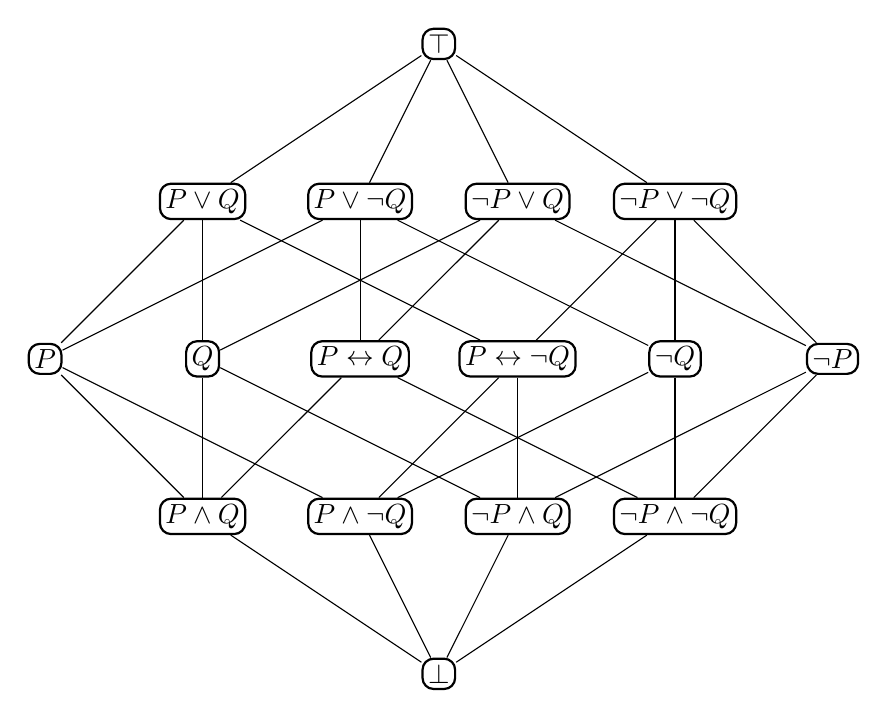
\begin{tikzpicture}[source/.style={draw,thick,rounded corners,inner sep=2pt}]
\node[source] (min) at (0,-1) {$\bot$};
\node[source] (A1) at (-3,1) {$P\wedge Q$};
\node[source] (A2) at (-1,1) {$P\wedge \neg Q$};
\node[source] (A3) at (1,1) {$\neg P\wedge Q$};
\node[source] (A4) at (3,1) {$\neg P\wedge \neg Q$};
\node[source] (B1) at (-5,3) {$P$};
\node[source] (B2) at (-3,3) {$Q$};
\node[source] (B3) at (-1,3) {$P\leftrightarrow Q$};
\node[source] (B4) at (1,3) {$P\leftrightarrow \neg Q$};
\node[source] (B7) at (3,3) {$\neg Q$};
\node[source] (B8) at (5,3) {$\neg P$};
\node[source] (C1) at (-3,5) {$P\vee Q$};
\node[source] (C2) at (-1,5) {$P\vee \neg Q$};
\node[source] (C3) at (1,5) {$\neg P\vee Q$};
\node[source] (C4) at (3,5) {$\neg P\vee \neg Q$};
\node[source] (max) at (0,7) {$\top$};
\draw (min) -- (A1);
\draw (min) -- (A2);
\draw (min) -- (A3);
\draw (min) -- (A4);
\draw (A1) -- (B1);
\draw (A1) -- (B3);
\draw (A1) -- (B2);
\draw (A2) -- (B1);
\draw (A2) -- (B4);
\draw (A2) -- (B7);
\draw (A3) -- (B2);
\draw (A3) -- (B4);
\draw (A3) -- (B8);
\draw (A4) -- (B3);
\draw (A4) -- (B8);
\draw (A4) -- (B7);
\draw (B1) -- (C1);
\draw (B1) -- (C2);
\draw (B2) -- (C1);
\draw (B2) -- (C3);
\draw (B3) -- (C2);
\draw (B3) -- (C3);
\draw (B4) -- (C1);
\draw (B4) -- (C4);
\draw (B7) -- (C2);
\draw (B7) -- (C4);
\draw (B8) -- (C3);
\draw (B8) -- (C4);
\draw (C1) -- (max);
\draw (C2) -- (max);
\draw (C3) -- (max);
\draw (C4) -- (max);
\end{tikzpicture}
\caption{Horizontal rows have the same number of $1$'s.  A connecting line indicates logical implication going upwards.} \label{hasse} 
\end{figure}

Since we have equivalences:
\[ P\to Q \equiv \neg P\vee Q \qquad \text{and} \qquad P\wedge Q
  \equiv \neg (\neg P\vee \neg Q) , \] any sentence is equivalent to a
sentence whose only connectives are $\vee$ and $\neg$, and each of the $16$ truth
functions can be expressed in terms of these connectives.  Similarly,
each of these $16$ truth functions can be expressed just with $\neg$
and $\wedge$.  If every truth-function
can be expressed in terms of a set $\Gamma$ of connectives, then we
say that $\Gamma$ is \emph{\gls{expressively complete}} or
\emph{expressively adequate}.  Thus, we just sketched proofs that
$\{ \neg ,\vee\}$ and $\{ \neg ,\wedge\}$ are expressively complete.

Amazingly, there is a single truth-function that is itself
expressively complete.  The corresponding connective is called
``nand'', and is usually symbolized by $\uparrow$.  The truth-table
for $P \uparrow Q$ is, by definition, the same as that for
$\neg (P\wedge Q)$.
\[ \begin{array}{ c@{\, }c | c@{\, }c@{\, }c }
P & Q   & P & \uparrow & Q  \\  \hline
1 & 1   & 1 & \mathbf{0} & 1  \\
1 & 0   & 1 & \mathbf{1} & 0  \\
0 & 1   & 0 & \mathbf{1} & 1  \\
0 & 0   & 0 & \mathbf{1} & 0  \\
\end{array} \]
To show that the set $\{ \uparrow \}$ is expressively complete, it will suffice
to show that it can reproduce the truth tables for $\neg$ and $\vee$.
After some trial and error, we find that the following definitions work:
\[ \begin{array}{c c c c } \begin{array}{ c | c@{\, }c@{\, }c}
P & P & \uparrow & P  \\
\hline 
1 &   1 & \mathbf{0} & 1  \\
0 &   0 & \mathbf{1} & 0  \end{array} 
& & & \begin{array}{ c@{\, }c | c@{ }c@{\, }c@{\, }c@{ }c@{\, }c@{\, }c@{ }c@{\, }c@{\, }c@{ }c@{ }c@{ }c}
     P & Q &   ( & P & \uparrow & P & ) & \uparrow & ( & Q & \uparrow & Q & ) & \\
\hline 
1 & 1 &    & 1 & 0 & 1 &  & \mathbf{1} &  & 1 & 0 & 1 &  & \\
1 & 0 &    & 1 & 0 & 1 &  & \mathbf{1} &  & 0 & 1 & 0 &  & \\
0 & 1 &    & 0 & 1 & 0 &  & \mathbf{1} &  & 1 & 0 & 1 &  & \\
0 & 0 &    & 0 & 1 & 0 &  & \mathbf{0} &  & 0 & 1 & 0 &  & \\
      \end{array} \end{array} \]
  \begin{exercise} Give a formula using only $P,Q$ and $\uparrow$ that
    has the same truth-table as $P\wedge Q$. \end{exercise} If any
  truth-function can be expressed by the $\uparrow$ connective, then, why, you might wonder, don't we 
  use it, instead of the redundant collection $\{ \neg ,\vee ,\wedge
  ,\to \}$ of four connectives?  The answer, in short, is that we
  face a trade off between simplicity and naturality, where the latter
  is a function of what we are familiar with.  For most of us, it's
  fairly natural to reason in terms of ``and'', and less natural to
  reason in terms of ``nand''.  Why that is, we don't pretend to know.
  Nonetheless, you now know that if somebody has the concept of
  ``nand'', then they can express any other truth-functional concept.

It can be more difficult to show that a set of connectives is {\it
  not} expressively complete.  For example, suppose that we want to
show that the set $\{ \vee \}$ is not, by itself, truth-functionally
complete.  The way we would approach this is to start trying to
express some of the truth-tables, to get a feeling of what we {\it
  cannot} do.  With the connective $\vee$, we can write $P\vee P$,
which is equivalent to $P$ again.  We can also write $P\vee Q$.  But
it seems that we get stuck at that point.  If we write longer
disjunctions, say $P\vee (P\vee Q)$, we quickly realize that we
haven't expressed anything new.  That is, we get stuck with
truth-functions that are true whenever $P$ and $Q$ are true.  That
realization then gives us an idea: perhaps we can prove that every
truth-function that can be expressed with just $\vee$ has this
feature, i.e.\ that it's true whenever $P$ and $Q$ are true.  That
idea provides the intuition behind the following proof.

  To make this proof a bit more clear, we need a slight change of
  terminology.  Instead of talking about a row of a truth-table, let's
  talk about a \emph{valuation}.  To be precise, a valuation $v$
  assigns each atomic sentence (in this case, $P$ and $Q$) either $0$
  or $1$.  If we follow the truth-table recipe, then a valuation
  naturally extends to assign every sentence either $0$ or $1$.  For
  example, if $v(\phi )=1$ and $v(\psi )=1$ then $v(\phi\vee\psi
  )=1$.  The claim above, then, is that if $v$ is a valuation such
  that $v(P)=1$ and $v(Q)=1$, then $v(\phi )=1$ for any sentence whose
  only connective is $\vee$. 

\begin{prop} The set $\{ \vee\}$ is not truth-functionally
  complete. \end{prop}

\begin{proof} Let $\Gamma$ be the set of sentences built only with the
  connective $\vee$.  Let $v$ be the valuation that assigns $1$ to
  every atomic sentence.  We show that for every sentence
  $\phi\in\Gamma$, $v(\phi )=1$.  Our argument proceeds by induction
  on the construction of $\Gamma$.  By definition, for $\phi$ an
  atomic sentence in $\Gamma$, we have $v(\phi )=1$.  Furthermore, if
  $v(\phi )=1$ and $\phi (\psi )=1$ then $v(\phi\vee\psi )=1$.
  Therefore, $v(\phi )=1$ for all $\phi\in \Gamma$.  It follows that
  there is no sentence in $\Gamma$ that is logically equivalent to
  $P\wedge\neg P$, and $\{ \vee \}$ is not truth-functionally
  complete.
\end{proof}

\begin{exercise} 
Show that the set $\{ \wedge \}$ is not truth-functionally
complete. \end{exercise}
\begin{exercise} Consider sentences built out of the atomic sentences $P$ and
    $Q$.  In this case, there are four valuations $v_1,v_2,v_3,v_4$.
    Let's say that a sentence $\phi$ is a {\it even} just in case
    $\phi$ is true for either $0,2$, or $4$ valuations.  Show that if
    $\phi$ is even then $\neg \phi$ is even.  Show that if $\phi$ and
    $\psi$ are even, then $\phi\lra\psi$ is even. \end{exercise}
  \begin{exercise} Is the set $\{ \neg ,\lra \}$ truth-functionally
    complete? \end{exercise}

%% TO DO: draw sentences as subsets of the space of valuations

%% TO DO: prove $\vdash (P\lra Q)\vee (P\lra R)\vee (P\lra R)

%% TO DO: show that $P\lra (P\lra Q)\equiv Q$





%% TO DO -- define substitution instances

\section{A theory of what can be proven}

In the previous sections we developed a theory about the grammar and
semantics of propositional logic.  In this section we develop a theory
about proofs, i.e.\ about what can and cannot be proven with the
inference rules for propositional logic.  To this end, we introduce
into {\it our} language --- i.e.\ the language we are using to
describe propositional logic --- a relation symbol $\vdash$, which we
write in infix notation, taking an argument on the left and an
argument on the right.  (Technically, the symbol $\vdash$ ambiguously
represents several different relation symbols, one for each finite
number of sentences that can occur on the left.  But we'll brush this
complication under the rug.)

The inference rules for propositional logic provide an \emph{inductive
  definition} of the set of valid sequents, i.e.\ of the extension of
the relation $\vdash$.  \index{definition!inductive} The base case
here is the rule of assumptions: for any formula $\phi$, the sequent
$\phi\vdash\phi$ is valid.  Each of the other inference rules is a
recipe for constructing a new valid sequent from one, two, or three
old ones.  Since the extension of $\vdash$ is defined inductively, it
follows that we can prove things about all sequents by means of an
induction schema.  Here the induction schema looks like this:

\bigskip \begin{tcolorbox}[enhanced,width=12cm,title=Induction on the
  construction of sequents,attach boxed title to top
  left={yshift=-2mm,xshift=4mm},boxed title style={sharp corners}]
$ \begin{array}{c p{7cm} p{2.3cm}}
     (1) & $\phi\vdash\phi$ has property $X$. & base \\
     (2) & If $\Gamma\vdash \phi\to\psi$ and
           $\Gamma\vdash\phi$ have property
           $X$, \newline then $\Gamma\vdash\psi$ has property $X$. &
                                                                     induction MP  \\
     \vdots \\ \hline
     (\text{C}) & All sequents have property
                  $X$. & conclusion \end{array} $ \end{tcolorbox} As
              you can see, a proof by induction on the construction of
              sequents will involve {\it many} inductive steps --- one
              for each inference rule.  But what kinds of things might
              we want to show about the collection of all sequents?
              There are two things about the collection of sequents
              that we've already assumed and used.  First, we assumed
              that sequents couldn't be messed up by find-and-replace
              operations.  That is, for any sequent
              $\phi\vdash\psi$, if you perform a uniform substitution
              of sentences for propositional constants, then you get
              another valid sequent $F(\phi )\vdash F(\psi )$.  Second, we assumed that truth-tables can detect when a sequent cannot be proven.  In other words, we assumed that for any valid sequent $\phi\vdash\psi$, the truth table for $\phi$ and $\psi$ will have no row in which $\phi$ is true and $\psi$ is false.  It's time now to prove that these two assumptions are true.

In order to set up these proofs, it will be helpful to imagine two
different languages, with different atomic sentences.  Let $\Sigma$ be
one list of atomic sentences, and let $\Sigma '$ be another list of
atomic sentences.  We call $\Sigma$ the \emph{\gls{signature}}
\index{signature} of the one language, whereas $\Sigma '$ is the
signature of the second language.  (If it helps you to remember, you
could think of $\Sigma '$ as having atomic sentences that have a prime
symbol, say $P',Q',R'$.)  We then let both languages build their
sentences from their respective atomic sentences using the logical
connectives $\neg ,\wedge ,\vee ,\to$.

Now let's imagine what might count as a \emph{\gls{translation}}
\index{translation} between languages $\Sigma$ and $\Sigma '$.  Keep
in mind that a good translation between languages need not be
word-for-word.  For example, it's doubtful that there is a single
English word that could translate the German word {\it Zeitgeist}, or
a single English word that could translate the Danish word {\it
  hygge}.  (I've hear that there are many more interesting examples
from languages such as Hindi, Urdu, and Mandarin.)  So, we shouldn't
require that a translation from $\Sigma$ to $\Sigma '$ has to match an
atomic sentence in $\Sigma$ with an atomic sentence in $\Sigma '$.
Instead, we will allow that an atomic sentence in $\Sigma$ be
reconstrued as {\it any} sentence of $\Sigma '$.

\begin{defn} Let $\Sigma$ and $\Sigma '$ be propositional signatures.
  A \emph{\gls{reconstrual}} $F$ from $\Sigma$ to $\Sigma '$ is a
  function that takes atomic sentences of $\Sigma$ to sentences of
  $\Sigma '$.  \end{defn}

A reconstrual $F:\Sigma\to\Sigma '$ extends naturally to a function
from {\it all} sentences of $\Sigma$ to sentences of $\Sigma '$.  We define:
\[ \begin{array}{r c l}
     F(\neg \phi ) & = & \neg F(\phi ) , \\
     F(\phi\wedge\psi ) & = & F(\phi )\wedge F(\psi ) , \\
     F(\phi\vee\psi ) & = & F(\phi )\vee F(\psi ) ,\\
     F(\phi\to\psi ) & = & F(\phi )\to F(\psi ) .\end{array} \] To get
 a feel for how this extension works, lets look at a specific example.  Suppose that $\Sigma = \{ P,Q\}$, $\Sigma '=\{ R,S\}$, and that we define the reconstrual $F$ by $F(P)=R\wedge S$ and $F(Q)=\neg S$. Then
\[ F(\neg P\vee Q ) \: = \: \neg F(P)\vee F(Q) =\neg (R\wedge S)\vee \neg S
  . \]

While a translation $F$ can run between distinct languages, it can
also run from a language back to itself.  This kind of thing happens,
in fact, quite frequently in the sciences.  For example, a few decades
ago, some clever economists figured out that some of the differential
equations of physics could be applied to financial markets.  Their
proposal amounted to a translation from the language of physics into
the language of economics --- and since are both part of our total
language, a translation from our language back into itself.

Within propositional logic, we can use this notion of translating a
language into itself to make sense of the idea of a substitution
instance of a sentence.  In short, a substitution instance of a
sentence $\phi$ is any sentence to which $\phi$ could be translated.
(It can be helpful here to continue thinking of translations to other
languages.  In that case, a sentence in our language can have
substitution instances in many other different languages.)
\begin{defn} A \gls{substitution instance} of $\phi$ is any sentence
  of the form $F(\phi )$, where $F:\Sigma\to\Sigma '$ is a
  reconstrual. \end{defn} The key idea here is that a substitution
instance of a sentence has the {\it same form} as that sentence.  One
confirmation that we've got the notion right is that any substitution
instance of a tautology is still a tautology.  (Here we are using
``tautology'' in its semantic sense: a sentence that is true relative
to every valuation.)

\begin{prop} If $\phi$ is a tautology, then any substitution instance
  of $\phi$ is also a tautology. \end{prop}

\begin{proof} Suppose that $\phi$ is a tautology and that $F(\phi )$
  is a substitution instance of $\phi$.  Let $v$ be an arbitrary
  valuation.  We need to show that $v(F(\phi ))=1$.  Consider the
  valuation $w$ defined by $w(P)=v(F(P))$ for each atomic sentence
  $P$.  Since $\phi$ is a tautology, $w(\phi )=1$.  In addition, since
  $w$ and $v\circ F$ agree on atomic sentences, and both commute with
  all the sentence connectives, it follows that $w=v\circ F$.
  Therefore, $v(F(\phi ))=(v\circ F)(\phi )=w(\phi )=1$.  Since $v$
  was an arbitrary valuation, it follows that $F(\phi )$ is a
  tautology. \end{proof}

\begin{prop} If $\phi$ is a contingent sentence, then $\phi$ has a
  tautologous substitution instance. \end{prop}

\begin{proof} Suppose that $\phi$ is contingent, and let
  $P_0,\dots ,P_n$ be a list of the atomic sentences that occur in
  $\phi$.  Since $\phi$ is contingent, there is a valuation $v$ such
  that $v(\phi )=1$.  Let $F$ be an arbitrary contradiction, and let
  $T$ be an arbitrary tautology.  For $i=0,\dots ,n$, define
  $f(P_i)=T$ if $v(P_i)=1$, and $f(P_i)=F$ if $v(P_i)=0$.  We claim
  then that $f(\phi )$ is a tautology.  Let $w$ be an arbitrary
  valuation.  For each atomic sentence $P_i$, if $v(P_i)=1$ then
  $v(P_i)=w(T)=w(f(P_i))$; and if $v(P_i)=0$ then
  $v(P_i)=w(F)=w(f(P_i))$.  Thus, $v$ and $w\circ f$ agree on all
  atomic sentences.  Since $v$ and $w\circ f$ are truth-functional,
  they agree on all sentences, hence on $\phi$.  Therefore
  $w(f(\phi ))=v(\phi )=1$.  Since $w$ was an arbitrary valuation,
  $f(\phi )$ is a tautology. \end{proof}

\begin{exercise} Give a tautologous substitution instance
  of the sentence $P\to (Q\wedge R)$. \end{exercise}

\begin{exercise} Follow the outlines of the previous proof to show
  that if $\phi$ is a contingent sentence, then $\phi$ has an
  inconsistent substitution instance. \end{exercise}

We're now ready for the main show.  The substitution meta-rule says
that if you take a valid proof and perform uniform substitution, then
the result is still a valid proof.  We now prove that fact.

\begin{subthm} Let $F:\Sigma\to\Sigma '$ be a reconstrual.  If
  $\phi _1,\dots ,\phi _n\vdash \psi$ then
  $F(\phi _1),\dots ,F(\phi _n)\vdash F(\psi )$. \end{subthm} \index{substitution}

\begin{proof} We prove the result by induction on the construction of
  sequents.  (We will prove the inductive steps for $\wedge$I, CP, and
  $\vee$E, and leave the other steps to the reader.)

  \bigskip \noindent \fbox{base case} \, The rule of assumptions gives
  not only $\phi\vdash\phi$, but also $F(\phi )\vdash F(\phi )$.

  \bigskip \noindent \fbox{induction $\wedge$I} \, Suppose that
  $\phi _1,\dots ,\phi _n,\psi _1,\dots ,\psi _n\:\vdash\: \phi\wedge
  \psi$ results from an application of $\wedge$I to
  $\phi _1,\dots ,\phi _n\vdash\phi$ and
  $\psi _1,\dots ,\psi _n\vdash \psi$, and suppose that the result
  holds for these latter two sequents.  That is,
  $F(\phi _1),\dots ,F(\phi _n)\vdash F(\phi )$ and
  $F(\psi _1),\dots ,F(\psi _n)\vdash F(\psi )$.  By conjunction
  introduction, we have
   \[ F(\phi _1),\dots ,F(\phi _n),F(\psi _1),\dots
     ,F(\psi _n)\:\vdash\: F(\phi )\wedge F(\psi ) .\] Since
   $F(\phi )\wedge F(\psi )=F(\phi\wedge\psi)$, it follows that
   \[ F(\phi _1),\dots ,F(\phi _n),F(\psi _1),\dots ,F(\psi
     _n)\:\vdash\: F(\phi \wedge \psi ) .\]

   \bigskip \noindent \fbox{induction CP} \, Suppose that
   $\phi _1,\dots ,\phi _n\vdash \psi\to \chi$ is derived by CP from
   $\phi _1,\dots ,\phi _n,\psi\vdash \chi$.  Now assume that the
   result holds for the latter sequent, i.e.
   $F(\phi _1),\dots ,F(\phi _n),F(\psi )\vdash F(\chi )$.  Then CP
   yields
   \[ F(\phi _1),\dots ,F(\phi _n)\:\vdash\: F(\psi )\to F(\chi ) .\]
   Since $F(\psi )\to F(\chi )=F(\psi\to\chi )$, it follows that
   \[ F(\phi _1),\dots ,F(\phi _n)\:\vdash\: F(\psi\to\chi ) .\]

   \bigskip \noindent \fbox{induction RAA} \, Suppose that
   $\phi _1,\dots ,\phi _n\vdash\neg \psi$ is derived by RAA from
   $\phi _1,\dots ,\phi _n,\psi\vdash\chi\wedge\neg\chi$, and assume
   that the result holds for the latter sequent, i.e.
   $F(\phi _1),\dots ,F(\phi _n),F(\psi )\vdash F(\chi\wedge\neg\chi
   )$.  By the properties of $F$,
   $F(\chi\wedge\neg\chi )=F(\chi )\wedge\neg F(\chi )$, which is also
   a contradiction.  Thus, RAA yields
   $F(\phi _1),\dots ,F(\phi _n)\vdash \neg F(\psi )$.  Since
   $\neg F(\psi )=F(\neg \psi)$, it follows that
   $F(\phi _1),\dots ,F(\phi _n)\:\vdash\: F(\neg \psi )$, which is
   what we wanted to prove.

   \bigskip \noindent \fbox{induction $\vee$E} \, Suppose that
   $\phi ,\psi _1,\psi _2\vdash \chi$ results from an application of
   $\vee$E to the following three sequents:
   \[ \phi\vdash \theta _1\vee\theta _2 \qquad \psi _1,\theta _1\vdash
     \chi \qquad \psi _2,\theta _2\vdash \psi \] and assume that the
   result holds for the latter three sequents, that is
   \[ F(\phi )\vdash F(\theta _1\vee\theta _2) \qquad F(\psi _1
     ),F(\theta _1 )\vdash F(\chi ) \qquad F(\psi _2),F(\theta
     _2)\vdash F(\psi ) \] Since
   $F(\theta _1\vee\theta _2)=F(\theta _1)\vee F(\theta _2)$, an
   application of $\vee$E yields
\[ F(\phi ),F(\psi _1),F(\psi _2)\:\vdash\: F(\chi ) .\]

\bigskip \noindent As mentioned before, we leave the remaining step to
the interested reader.  With those steps completed, it follows that
for any sentences $\phi _1,\dots ,\phi _n,\psi$, if
$\phi _1,\dots ,\phi _n\vdash\psi$ then
$F(\phi _1),\dots ,F(\phi _n)\vdash F(\psi )$.
\end{proof}

The previous proposition immediately yields the following corollary.

\begin{prop} If $\phi$ is provable, then any substitution instance of
  $\phi$ is also provable. \end{prop}

We're now ready to prove the \gls{sound} of the inference rules for
propositional logic.  The proof is essentially another version of the
proof of the substitution theorem, except that we map sentences to the
numbers $0$ and $1$ instead of to other sentences.

\begin{sothm} For any valuation $v$, if
  $\phi _1,\dots ,\phi _n\vdash\psi$ then
  $\min \{ v(\phi _1),\dots ,v(\phi _n) \}\leq v(\psi )$.  \end{sothm}

In the statement of the theorem, ``$\min$'' treats the premises
$\phi _1,\dots ,\phi _n$ as forming a conjunction: the minimum of
$v_1(\phi _1),\dots ,v(\phi _n)$ is the same as
$v(\phi _1\wedge\cdots\wedge \phi _n)$.

\begin{proof} The proof is by induction on the construction of
  sequents.  We will just show a couple of cases, and leave the others
  to the reader.

  \bigskip\noindent \fbox{induction MP} \, Suppose that $\phi _1,\phi _2\vdash\chi$ results
  from MP applied to $\phi _1\vdash \psi\to\chi$ and $\phi
  _2\vdash\psi$.  Suppose also that $v(\phi _1)\leq v(\psi\to\chi )$
  and $v(\psi _1)\leq v(\psi )$.  If $\min \{ v(\phi _1),v(\phi _2)
  \}=0$, then we're done.  If $\min \{ v(\phi _1),v(\phi _2) \}=1$,
  then $v(\psi\to \chi )=1$ and $v(\psi )=1$, from which it follows
  that $v(\chi )=1$.  In either case, $\min \{ v(\phi _1),v(\phi
  _2)\}\leq v(\chi )$.   

  \bigskip\noindent \fbox{induction CP} \, Suppose that
  $\phi \vdash \psi\to \chi$ is derived by CP from
  $\phi ,\psi\vdash \chi$, and assume that the result holds for the
  latter sequent, i.e.
  $\min \{ v(\phi ),v(\psi ) \} \:\leq\: v(\chi )$. Either
  $v(\psi )=0$ or $v(\psi )=1$.  If $v(\psi )=0$ then
  $v(\psi\to\chi )=1$ and we're done.  If $v(\psi )=1$ then the above
  gives $v(\chi )=1$, and hence $v(\psi\to\chi )=1$.  In either case,
  $v(\phi )\leq v(\psi\to\chi )$.
\end{proof}

This fulfills the promise we made in Chapter \ref{truth} that the
truth table method provides a reliable test for when a sequent cannot
be proven.  In particular, if there is a row in the truth table where
$\phi$ is assigned $1$ and $\psi$ is assigned $0$, then the sequent
$\phi\vdash\psi$ cannot be proven.  Similarly, if there is a row in
the truth table where $\psi$ is assigned $0$, then $\vdash\psi$ cannot
be proven.

\begin{exercise} Prove the steps of the soundness theorem for the
  $\vee$I and $\vee$E rules. \end{exercise}
\begin{exercise} Show that if $\phi$ is inconsistent, then any
  substitution instance of $\phi$ is inconsistent.  Here we mean
  ``inconsistent'' in the semantic sense of being assigned $0$ by all
  valuations. \end{exercise}
\begin{exercise} Show that if $\phi$ is a contingent sentence, then $\phi$ has a
  contradictory substitution instance. \end{exercise}


\section{Disjunctive Normal Form}

What we want to do next is to prove the \gls{complete} theorem: if an
argument is truth-preserving, then it can be proven with our inference
rules.  That's actually a non-trivial theorem that was only discovered
in the early twentieth century.  So, to get there, we're going to need
to do some work.  We'll start with something that might seem to be
nothing but boring syntactic bookkeeping.  We define a particular kind
of form a sentence can take.  Then we show that every sentence is
provably equivalent to one with this particular kind of
form.\footnote{It's at this point where it becomes crucial that we
  have {\it enough} inference rules.  If we didn't have enough rules
  then not every sentence would be provably equivalent to one in this
  form.}  It turns out, however, that this fact is quite useful --- in
particular, because sentences in this form wear their inferential
relations on their sleeves.  (It's as if these sentences have an
address that shows where they live in logical space.)

\begin{defn} A sentence $\phi$ is in \gls{dnf} just in case it is a disjunction of
conjunctions of literals (atomic and negated atomic
sentences). \end{defn}

For example, the following sentences are DNF:
\[ P \qquad P\wedge \neg Q \qquad (P\wedge \neg Q)\vee (\neg P\wedge
  Q) \]
We can define the family of DNF formulas inductively as follows:
\begin{itemize}
\item All conjunctions of literals (atomic and negated atomic sentences) are DNF.
\item All disjunctions of DNF formulas are DNF.
\end{itemize}
The disjunctive normal form theorem will show that every propositional
logic sentence is provably equivalent to a DNF sentence.  That result
can be proven in a couple of different ways, and it's useful in a
couple of different ways.  On the one hand, one can prove the DNF
theorem directly by establishing a bunch of sequents, and then using
mathematical induction to generalize to all sentences.  In that case,
the DNF theorem is a useful as a step along the way to proving the
completeness theorem for propositional logic.  On the other hand, if
one has established the completeness theorem by some other means, then
it gives a quick proof of the DNF theorem.  In what follows, we'll
first sketch the argument from completeness to the DNF theorem.  Then
we'll sketch a direct proof of the DNF theorem.

Suppose first that if two sentences have the same truth table, then
they are provably equivalent.  (This supposition is a direct
consequence of the completeness theorem.)  Now given a sentence
$\phi$, we will construct a DNF sentence $\phi '$ from the truth-table
for $\phi$.  If $\phi$ is always false, i.e.\ it has $0$ in all rows
of the main column, then let $\phi '$ be the sentence
$P\wedge \neg P$.  Otherwise, for each row $i$ in which $\phi$ is
true, let $\psi _i$ be the conjunction of all the atomic sentences
that are assigned true in that row, along with the negations of all
the atomic sentences that are assigned false in that row.  Note that
$\psi _i$ is true on row $i$ of the truth table, and false on every
row $j\neq i$.  Finally, let $\phi '$ be the disjunction of all the
$\psi _i$ that we have just constructed.

It's obvious that $\phi '$ is DNF.  So we just need to show that
$\phi$ and $\phi '$ have the same truth table.  Suppose that we set
them side by side, and consider row $i$ of the truth table.  If $\phi$
is true on row $i$, then one of the disjuncts of $\phi '$ is
$\psi _i$, which is true on row $i$.  Hence $\phi '$ is true on row
$i$.  Conversely, if $\phi '$ is true on row $i$, then the disjunct
$\psi _i$ appears in it; and by construction $\phi$ is true on row
$i$.  Thus, we have shown that $\phi$ and $\phi '$ have the same truth
table.  If we assume completeness, it follows that $\phi$ and $\phi '$
are provably equivalent.

This somewhat abstract argument can be illustrated by means of an
example.  Consider the sentence $\phi\equiv (P\to R)\to (Q\wedge R)$.
If you write out the full truth table of $\phi$, you'll find that it's
true in rows 1,2,4, and 5, and false in all other rows.  Thus, the
above recipe yields the sentence
\[ (P\wedge Q\wedge R)\vee (P\wedge Q\wedge\neg R)\vee (P\wedge\neg
  Q\wedge \neg R)\vee (\neg P\wedge Q\wedge R) \] It's pretty easy to
see here that $\phi '\vdash \phi$.  If one performed a big disjunction
elimination, then the first and fourth disjuncts immediately yield
$Q\wedge R$, and positive paradox yields $\phi$.  The second and third
disjuncts yield $P\wedge\neg R$, hence $\neg (P\to R)$, and then
$\phi$ by negative paradox.  Since $\phi '$ is a disjunction, it's a
bit more difficult to see that $\phi\vdash \phi '$.  However, you'll
recall that $\phi$ entails $\neg (P\to R)\vee (Q\wedge R)$, which in
turn entails $(P\wedge\neg R)\vee (Q\wedge R)$.  This last formula is
actually in DNF; and although not strictly identical to $\phi '$, it's
not hard to see how it's related to $\phi '$.

Making liberal use of known equivalences, we can rewrite $\phi '$ as
\[ \begin{array}{l} (P\wedge \neg R\wedge Q)\vee (P\wedge \neg R\wedge
    \neg Q)\vee
     (Q\wedge R\wedge P)\vee (Q\wedge R\wedge \neg P)  \\
     \dashv\vdash [(P\wedge \neg R)\wedge (Q\vee \neg Q)]\vee
     [(Q\wedge
     R)\wedge (P\vee \neg P)] \\
     \dashv\vdash (P\wedge \neg R)\vee (Q\wedge R) \end{array} \] This
example shows that DNF equivalent forms are not generally unique.

We now turn to the argument for the DNF theorem.  Actually, it's
easiest to prove something stronger, for which we need another
definition.

\begin{defn} A sentence is in \gls{cnf} just in case it's a
  conjunction of disjunctions of literals. \end{defn}

\begin{dnf} Every sentence $\phi$ is provably equivalent to a sentence
  $\phi ^d$ in disjunctive normal form, and to a sentence $\phi ^c$ in
  conjunctive normal form.  \end{dnf} 

\begin{proof} We argue by induction on the construction of sentences.
\begin{itemize}
\item Each atomic sentence is both in DNF and in CNF.
\item Suppose that $\phi$ is equivalent to $\phi ^c$ and to $\phi ^d$.
  Then $\neg \phi$ is equivalent to $\neg \phi ^d$, which has the form
  $\neg (\psi _1\vee\cdots\vee\psi _n)$.  By DeMorgan's rule, the
  latter is equivalent to
  $\neg \psi _1\wedge \cdots \wedge\neg \psi _n$.  By another
  application of DeMorgan's, each $\neg \psi _i$ is equivalent to a
  disjunction of literals.  Putting everything together,
  $\neg \phi ^d$ is equivalent to a CNF sentence.  A similar argument
  shows that $\neg \phi$ is equivalent to $\neg \phi ^c$, which is
  equivalent to a DNF sentence.  Therefore, $\neg \phi$ is equivalent
  to sentences in both CNF and DNF.
\item For disjunction and conjunction, we first note that $\vee$
  trivially preserves the family of DNF sentences, and $\wedge$
  trivially preserves the family of CNF sentences.  Thus, if $\phi$
  and $\psi$ are sentences that satisfy the hypothesis of the theorem,
  then $\phi\vee\psi$ is equivalent to a DNF sentence.  It's also
  equivalent to $\neg (\neg \phi\wedge\neg\psi )$, which is equivalent
  to a CNF sentence.  A similar argument shows that $\phi\wedge\psi$
  is equivalent to DNF and CNF sentences.
\item For conditionals, we have
  $\phi\to\psi\dashv\vdash\neg \phi\vee\psi$.  By the previous two
  steps, if $\phi$ and $\psi$ satisfy the hypotheses of the theorem,
  so does $\neg\phi\vee\psi$.
\end{itemize} \end{proof}

\begin{exercise} Go back through the proof of the DNF theorem and
  identify each provable equivalence that was cited.  Now identify
  which inference rules are needed to prove those equivalences.  Are
  any of the primitive rules of inference not needed for the proof to
  go through? \end{exercise}

What use is it that every sentence is equivalence to a DNF sentence?
For one, it gives us a quick way of understanding all the different
possible logical relations between sentences.  Consider, for example,
the case of all sentences whose only atomic sentence is $P$.  In this
case, the only literals are $P$ and $\neg P$, and every elementary
conjunction is equivalent to $P$, $\neg P$, or $P\wedge\neg P$.
Consequently, the DNF formulas are equivalent to
$P,\neg P,P\wedge\neg P$, or $P\vee\neg P$.  That is, every sentence
is logically equivalent to one of these four sentences.  

Furthermore, if two sentences $\phi,\psi$ are in DNF, then it can be
quite easy to see whether or not $\phi\vdash\psi$.  In short,
$\phi\vdash\psi$ just in case $\phi$ contains a conjunction which is
as long as some conjunction in $\psi$.  Consider, for example, the two
DNF formulas:
\[ Q\wedge P \qquad Q\vee (\neg Q\wedge \neg P) \] A quick inspection
shows that $\phi\vdash\psi$, since $Q\wedge P\vdash Q$ by conjunction
elimination, and $Q\vdash\psi$ by disjunction introduction.

We saw above that if $\phi$ is a sentence containing only $P$, then
$\phi$ is equivalent to one of the four sentences
$P,\neg P,\top ,\bot$.  If you took some time writing out formulas in
DNF, you'd also see that for sentences containing both $P$ and $Q$,
there are $16=2^4$ possibilities.  (There are $4$ consistent
elementary conjunctions:
\[ P\wedge Q \quad P\wedge \neg Q \quad \neg P\wedge Q \quad \neg
  P\wedge\neg Q ,\] then all possible disjunctions of those.)  In
general, if there are $n$ atomic sentences, then there are $2^{2^n}$
possible sentences up to logical equivalence.  Unsurprisingly,
$2^{2^n}$ is also the number of distinct truth-functions on $n$
inputs.  (Each distinct sentence corresponds to a distinct
truth-function.)

%% TO DO: it would be nice to elaborate a bit on the above counting
%% procedure.  How many elementary conjunctions?

Practically speaking, it's doubtful that you'll ever need to transform
a sentence into \gls{dnf} or \gls{cnf}.  In fact, you can have a
computer do that task for you.  But how, you might wonder, could you
write a program to convert sentences to DNF?  On the one hand, you
could program the computer first to compute a truth table, and then to
use the rows of the truth table to construct a corresponding formula.
On the other hand, you could program the computer to perform a series
of syntactic manipulations on the relevant formula.  Here's one sort
of algorithm you could use:
\begin{itemize}
\item Replace all instances of $\phi\to \psi$ with
  $\neg\phi\vee \psi$.
\item Whenever $\neg$ is prefixed to a conjunction or disjunction, use
  DeMorgan's equivalences to drive $\neg$ inwards.
\item Whenever $\wedge$ is applied to a disjunction, use distribution
  to transform to a disjunction of conjunctions.  
\end{itemize}
In order to trust such an algorithm, you would want to prove that it
will always terminate --- after a finite number of steps --- in a DNF
formula.  

\section{Completeness}

The claim here is that we have sufficiently many derivation rules to
be able to prove everything that we want to prove --- in particular,
all truth-preserving arguments.  Before we prove that, however, we can
show already that we couldn't add any more inference rules --- at
least not if we want to maintain soundness.  That is, if we add any
more inference rules, then we'll be able to prove an argument that is
{\it not} truth preserving.

We first need to be clear about what it would mean to add a ``new''
inference rule.  For example, suppose that I proposed adding the
following inference rule, viz.\ DeMorgan's Rule:
\[ \begin{array}{r c l} \Gamma & \vdash & \neg (\phi\vee\psi ) \\
    \hline \Gamma & \vdash & \neg\phi\wedge\neg\psi \end{array} \] I
might think myself very clever for coming up with a plausible new
inference rule.  The problem here, though, is that the rule isn't
really new: it can be derived from the rules that we already have.
Indeed, we've already proven that
$\vdash \neg (\phi\vee\psi )\to \neg\phi\wedge\neg\psi$.  So suppose
now that you were given a derivation that begins with assumptions
$\Gamma$, and that ends with $\neg (\phi\vee\psi )$.  Then you could
append the derivation of that conditional, perform a step of MP, and
that would yield a proof of $\neg\phi\wedge\neg\psi$, depending on
$\Gamma$.  In other words, $\Gamma\vdash \neg (\phi\vee\psi )$ can
always be converted to $\Gamma\vdash\neg\phi\wedge\neg\psi$.

A genuinely new derivation rule, then, would have to be a rule that
permits a derivation of a sentence $\phi$, without any remaining
dependencies, whereas $\phi$ previously was not derivable.  In other
words, $\not\vdash\phi$, where $\vdash\phi$ means that there is a
derivation of $\phi$ using the previous rules.

\begin{prop} If $\phi$ is not provable, then there is a substitution
  instance of $\phi$ that is provably equivalent to
  $\bot$. \end{prop}

\begin{proof} To illustrate the idea behind the proof, we'll consider
  first the case where the only atomic sentence in $\phi$ is $P$.  If
  $\phi$ is not provable, then $\phi$ must be provably equivalent to
  $P,\neg P$, or $\bot$.  In the last case, the result is trivially
  true.  But if $\phi$ is equivalent to $P$, then the substitution
  $F(P)=\bot$ will do.  If $\phi$ is equivalent to $\neg P$, then the
  substitution $F(P)=\top$ will do.

  For the general case, suppose that the atomic sentences in $\phi$
  are $P_1,\dots ,P_n$.  By the DNF theorem, $\phi$ is equivalent to a
  disjunction of elementary conjunctions of the $P_i$.  If $\phi$ is
  equivalent to a disjunction of all $2^n$ distinct elementary
  conjunctions, then $\phi$ is provable.  Since $\phi$ was assumed not
  to be provable, at least one of those $2^n$ conjunctions doesn't
  occur in $\phi ^d$.  Without loss of generality, suppose that
  $P_1\wedge\cdots\wedge P_n$ doesn't occur in $\phi ^d$.  Now let
  $F(P_i)=\top$ for $i=1,\dots ,n$.  Then each disjunct $\psi$ that
  occurs in $\phi ^d$ contains $\neg P_j$ for some $j$, and since
  $F(\neg P_j)=\neg\top$, it follows that
  $F(\psi )\vdash F(\neg P_j)\vdash\bot$.  Therefore
  $F(\phi )\vdash\bot$, and $F(\phi )$ is the desired substitution
  instance of $\phi$.
\end{proof}

We can now show that if we added a new inference rule, then we could
prove anything whatsoever.\footnote{This result is usually called
  \emph{Post completeness} in honor of the logician Emil Post
  (1897--1954).}  If there were a new inference rule, then we could
prove some sentence $\phi$ that was not previously provable.
Importantly, it's not just that we could prove $\phi$, but that we
could prove any substitution instance $F(\phi )$ of $\phi$.  Since
$\phi$ wasn't previous provable, there is a substitution instance
$F(\phi )$ of $\phi$ such that $\vdash F(\phi )\lra \bot$.  But then
we could prove $\bot$, and since $\bot\vdash\psi$ for all sentences
$\psi$, we could prove anything whatsoever.

We can now prove the completeness theorem.  For this, we use the
convenient notation $\phi\;\gls{double turnstile}\;\psi$ to mean that for any valuation
$v$, if $v(\phi )=1$ then $v(\psi )=1$.  In other words,
$\phi\vDash\psi$ means that the argument with premise $\phi$ and
conclusion $\psi$ is truth-preserving.

\begin{lemma*} If $\phi$ is not provable, then there is a valuation
  $v$ such that \mbox{$v(\phi )=0$}. \end{lemma*}

\begin{proof} Go through the preceding proof, replacing each case of
  $F(P)=\top$ with $v(P)=1$, each case of $F(P)=\bot$ with $v(P)=0$,
  and each case of $F(\phi )\equiv \bot$ with $v(\phi
  )=0$.  \end{proof}

\begin{fct} If $\phi\vDash\psi$ then $\phi\vdash\psi$.  \end{fct}

\begin{proof} We argue for the contrapositive.  Suppose that
  $\phi\not\vdash\psi$.  Then \mbox{$\not\vdash \phi\to\psi$}.  By the
  lemma, there is a valuation $v$ such that $v(\phi\to\psi )=0$.
  Therefore $v(\phi )=1$ and $v(\psi )=0$, which means that
  $\phi\not\vDash\psi$. \end{proof}

The finite completeness theorem tells you that if an argument is
truth-preserving, then there is a proof.  But it doesn't give you a
recipe for finding that proof.  In that sense, completeness is a {\it
  non-constructive} result: it shows $\exists x\phi (x)$ without
producing some $a$ such that $\phi (a)$.  In the case of propositional
logic, it's possible to redo the proof of completeness so that it
really is constructive --- i.e.\ it takes the relevant truth table, and
builds a proof (that might be long and ugly).  However, our goal here
is not to give you a recipe for outsourcing the job of proving to a
computer.

There's another really interesting thing we could prove about
propositional logic, but it's significantly more mathematically
demanding, since it deals with infinite sets.  Imagine that we had a
language with infinitely many atomic sentences $P_0,P_1,\dots $, in
which case there aren't just infinitely many distinct sentences, there
are also infinitely many logically inequivalent sentences.  Let's now
suppose that $\Gamma$ is any set of sentences, possibly an infinite
set.  We write $\Gamma\vDash\phi$ just in case any valuation that
makes {\it all} the sentences in $\Gamma$ true also makes $\phi$ true.
We write $\Gamma\vdash\phi$ just in case there is a proof that begins
with some finite number of sentences from $\Gamma$, and that ends with
$\phi$.  Now we can raise the question: does completeness continue to
hold in this more general case?

The answer is yes, provided that we help ourselves to an additional
assumption about sets of sentences.  This assumption can be formulated
in various ways; for example:
\begin{description}
\item[\textbf{Compactness (C)}] If a set $\Delta$ of sentences is inconsistent,
  then some finite subset $\Delta _0$ of $\Delta$ is already
  inconsistent.  (Here we are describing a semantic notion of
  inconsistency.)
\item[\textbf{Grow (G)}] If a set $\Gamma$ of sentences does not imply
  $\bot$, then it's contained in a set $\Gamma ^*$ that is maximal
  with respect to this property.  (Here we are describing a syntactic
  notion of consistency.)
\end{description}
The \textbf{Grow} axiom makes a lot of sense.  Imagine that your
current state of belief was represented by the set $\Gamma _0$; and
image that you are fortunate enough that your beliefs don't imply a
contradiction.  Then, the second assumption says that your set of
beliefs could grow to the limit point $\Gamma$ where you couldn't add
any more without falling into contradiction.  That idea doesn't just
make sense, it seems obviously true.

We now show that \textbf{C} is equivalent to \textbf{G}.  Suppose
first that \textbf{C} is true, and let $\Gamma$ be a set of sentences
that does not imply $\bot$. Thus, no finite subset $\Gamma _0$ of
$\Gamma$ implies $\bot$.  By the finite completeness theorem, every
finite subset $\Gamma _0$ of $\Gamma$ is semantically consistent.
Therefore by \textbf{C}, $\Gamma$ is semantically consistent, i.e.\
there is a valuation $v$ that assigns $1$ to every sentence in
$\Gamma$.  Let $\Gamma ^*$ be the set of all sentences that are
assigned $1$ by $v$.  If $\Gamma ^*\vdash\bot$, then soundness would
fail.  Therefore, $\Gamma ^*\not\vdash\bot$.  If
$\phi\not\in\Gamma ^*$, then $v(\phi )=0$ and $v(\neg \phi )=1$.
Hence $\neg\phi\in\Gamma ^*$, from which it follows that
$\Gamma ^*\cup \{ \phi\}\vdash\bot$.  Therefore, $\Gamma ^*$ is
maximally consistent (in the syntactic sense).

Suppose now that \textbf{G} is true.  We're going to show first that
for any set $\Delta$, if $\Delta\not\vdash\bot$ then $\Delta$ is
consistent.  Suppose then that $\Delta\not\vdash\bot$.  By \textbf{G},
$\Delta\subseteq\Gamma$, where $\Gamma\not\vdash\bot$, and if
$\phi\not\in\Gamma$ then $\Gamma\cup \{\phi\}\vdash\bot$.  We claim
then that $\Gamma$ is the set of sentences that are assigned $1$ by
some valuation.
\begin{itemize}
\item We show that if $\Gamma\vdash\phi$ then $\phi\in \Gamma$.
  Suppose that $\Gamma\vdash\phi$.  If
  $\Gamma\cup \{ \phi \}\vdash\bot$ then $\Gamma\vdash\neg\phi$, hence
  $\Gamma\vdash\bot$, contrary to what we assumed about $\Gamma$.
  Therefore, $\Gamma\cup\{\phi \}\not\vdash\bot$, and by maximality,
  $\phi\in\Gamma$.
\item We show that if $\Gamma\not\vdash\phi$ then $\neg\phi\in\Gamma$.
  Suppose that $\Gamma\not\vdash\phi$.  If
  $\Gamma\cup \{ \neg \phi \}\vdash\bot$ then
  $\Gamma\vdash\neg\neg \phi$, and hence $\Gamma\vdash\phi$, contrary
  to our assumption.  Therefore,
  $\Gamma\cup \{\neg \phi \}\not\vdash\bot$, and by maximality,
  $\neg\phi\in\Gamma$.
\item We show now that $\phi\wedge\psi\in\Gamma$ iff $\phi\in\Gamma$
  and $\psi\in\Gamma$.  If $\phi\wedge\psi\in\Gamma$ then
  $\Gamma\vdash\phi$ and $\phi\in\Gamma$.  Similarly,
  $\Gamma\vdash\psi$ and $\psi\in\Gamma$.  Conversely, if
  $\phi\in\Gamma$ and $\psi\in\Gamma$ then $\Gamma\vdash\phi$ and
  $\Gamma\vdash\psi$, therefore $\Gamma\vdash\phi\wedge\psi$ and
  $\phi\wedge\psi\in\Gamma$.
\item We show that $\phi\vee\psi\in\Gamma$ iff either $\phi\in\Gamma$
  or $\psi\in\Gamma$.  If $\phi\not\in\Gamma$ and $\psi\not\in\Gamma$
  then $\neg\phi\in\Gamma$ and $\neg\psi\in\Gamma$, from which it
  follows that $\neg\phi\wedge\neg\psi\in\Gamma$.  But then
  $\neg (\phi\vee\psi)\in\Gamma$, which means that
  $\phi\vee\psi\not\in\Gamma$.  Conversely, if $\phi\in\Gamma$, then
  $\Gamma\vdash\phi$, from which $\Gamma\vdash\phi\vee\psi$, and
  therefore $\phi\vee\psi\in\Gamma$.  \end{itemize} We can then define
$v(\phi )=1$ iff $\phi\in\Gamma$, and it follows that $v$ is a
well-defined valuation.  Therefore, $v$ assigns $1$ to all sentences
in $\Delta$, and $\Delta$ is consistent.

By the previous argument, if $\Delta$ is inconsistent, then
$\Delta\vdash\bot$.  But if $\Delta\vdash\bot$ then
$\Delta _0\vdash\bot$ for some finite subset $\Delta _0$ of $\Delta$.
By soundness, $\Delta _0$ is inconsistent, which completeness the
derivation of \textbf{C} from \textbf{G}.

Let's check now that \textbf{C} plus finite completeness implies
general completeness.  If $\Gamma\vdash\psi$, then
$\Gamma\cup\{\neg\psi \}$ is inconsistent.  By compactness, there is a
finite subset $\{ \phi _1,\dots ,\phi _n\}$ of $\Gamma$ such that
$\{ \phi _1,\dots ,\phi _n, \neg \psi\}$ is inconsistent, and hence
$\phi _1,\dots ,\phi _n\vDash\psi$.  By the finite completeness
theorem, $\phi _1,\dots ,\phi _n\vdash\psi$, which means that
$\Gamma\vdash\phi$.

Some day you might find another logic book that claims to prove
compactness.  Why then would we assume compactness, when it can be
proven to be true?  In this case, proofs of compactness assume not
only the axioms of set theory, but an additional axiom which goes
under various names, such as ``the axiom of choice'' and ``Hausdorff's
maximal principle.''  Those latter axioms are like industrial strength
power tools, designed to crack some of the hardest mathematical
puzzles.  For an introductory book, we don't need such heavy-duty
set-theoretic assumptions.  Nonetheless, you might be interested to
know that compactness for propositional logic is provably equivalent
to some other well-known mathematical facts.  First, if you take a
course in abstract algebra, you'll learn that each Boolean ideal can
be extended to a prime ideal (the Boolean prime ideal theorem).  That
fact is very similar to our ``grow'' axiom, and it is indeed provably
equivalent to compactness.  Similarly, if you take a course in graph
theory, you might learn that in a tree $T$ with infinitely many nodes,
if each node has only finitely many children, then $T$ has a branch of
infinite length (K\"onig's lemma).  That fact is also provably
equivalent to compactness.

The compactness property can seem a bit paradoxical.  Consider, for
example, the following apparently valid argument with infinitely many
premises.
\[ \begin{array}{p{5.3cm}}
     There is more than one angel.     \\
     There are more than two angels.     \\
     \vdots \\ \hline There are infinitely many angels. \end{array} \]
 If this argument is valid, then compactness entails that the conclusion is a logical
 consequence of only finitely many of the premises.  In particular,
 there is a largest natural number $n$ such that the premise ``there
 are more than $n$ angels'' implies the conclusion ``there are
 infinitely many angels,'' which seems obviously wrong.  The solution
 to this little puzzle is simply that propositional logic renders a
 false verdict about the structure of this argument.  But that
 shouldn't be surprising; we already know that propositional logic
 provides only a partial picture of what makes arguments valid.

%% TO DO: formation rules for predicate logic

%% TO DO: how to formula substitution for predicate logic

%% TO DO: prove soundness of some of the quantifier rules




\begin{exercises} \mbox{}
  \begin{enumerate}
  \sitem Let $T$ stand for the system of propositional logic with
  connectives $\neg ,\wedge$, and with rules $\wedge$I, $\wedge$E,
  RAA, and DN.  We write $\succ\phi$ to indicate that $\phi$ is
  provable in system $T$.  Either prove or refute the following
  statement: for a sentence $\phi$ that contains only $\neg$ and
  $\wedge$, if $\vdash\phi$ then $\succ\phi$.

  \sitem In this exercise, you're asked to show that the RAA rule is
  redundant.  Let $T$ stand for the system of propositional logic that
  results from dropping the RAA rule, and write $\phi\succ\psi$ to
  indicate that the corresponding sequent is provable in system $T$.
  Show that if $\phi\vdash\psi$ then $\phi\succ\psi$.  (Hint: prove
  that $P\to \neg P\succ\neg P$.)

\item Show that the DN introduction rule is redundant, i.e.\ is
  derivable from the remaining rules in our system.

\item Show that MT is redundant, i.e.\ is derivable from the
  remaining rules in our system.

  \sitem Show that the set of Stage $0$ rules of inference (i.e.\
  those given in the ``Deducing'' chapter) is incomplete.  Hint:
  construct an alternate truth-table for $\vee$, and show that the
  Stage $0$ rules are sound relative to that truth table.

\sitem Give introduction and elimination rules for the nand
  connective $\uparrow$.  Prove that your rules are sound relative to
  the truth-table for $\uparrow$.

\end{enumerate} \end{exercises}

%% should I talk about Compactness? 

%% TO DO: Show that RAA is eliminable.  Show that MTT is eliminable.

%% Post Completeness



\newglossaryentry{contingent sentence}
{
  name={contingent sentence},
  description={A sentence is contingent if there is an interpretation
    in which its true, and an interpretation in which its false}
}


%% TO DO: truth functionality
%% expressive completeness
%% 

%%% Local Variables:
%%% mode: latex
%%% TeX-master: "main"
%%% End:




% [[In some systems of propositional logic, there is a special symbol
% $\bot$, which is taken to be a name of a specific sentence: the
% always-false sentence.  One can then define a couple of new inference
% rules to use with this symbol.  The $\bot$ introduction rule says that
% whenever you have sentences $\phi$ and $\neg\phi$ on previous lines,
% then you can write $\bot$, aggregating the dependencies of $\phi$ and
% $\neg\phi$.  The $\bot$ elimination rule is just another version of Ex
% Falso Quodlibet.  It says that if you have $\bot$ on a line, then you
% can write any sentence on the next line, depending on whatever $\bot$
% depended upon.

% Having the $\bot$ symbol with its introduction and elimination rules
% can streamline several of our arguments.  For example, consider the
% following slightly streamlined proof for $P\vee Q,\neg P\vdash Q$.
% \[ \begin{array}{l l l p{2cm}}
%      1 & (1) & P\vee Q & A \\
%      2 & (2) & \neg P       & A \\
%      3 & (3) & P       & A \\
%      2,3 & (4) & \bot  & 2,3 $\bot$I \\
%      2,3 & (5) & Q     & 4 $\bot$E \\
%      6   & (6) & Q     & A \\
%      1,2 & (7) & Q     & 1,3,5,6,6 $\vee$E \end{array} \]

% We will show here that $\bot$ can be defined, and that the $\bot$
% introduction and elimination rules can be derived from the rules we
% already have.  We begin with the definition:
% \[ \bot \: \equiv \: P\wedge \neg P .\]
% (In fact, you could use any other atomic sentence you wanted to in this
% definition.)  The $\bot$ introduction rule looks like this:
% \[ \begin{array}{c} \phi \:\vdash\: \theta \qquad \psi \:\vdash \:\neg
%     \theta \\ \hline \phi ,\psi \:\vdash\: \bot \end{array} \] To
% derive this rule, it will suffice then to show that
% $\theta\wedge \neg\theta\vdash P\wedge\neg P$.  But of course, that
% follows from Ex Falso Quodlibet, which we have already derived.

% The $\bot$ elimination rule looks like this:
% \[ \begin{array}{c} \phi\:\vdash\:\bot \\ \hline
%     \phi\:\vdash\:\psi \end{array} \] To derive this rule, it will
% suffice to show that $\bot\vdash\psi$, for any sentence $\psi$.  But
% again, that follows from Ex Falso Quodlibet.]]

\chapter{A Theory about Predicate Logic} \label{meta2}

In this chapter we sketch the outlines of a theory predicate logic ---
or what's usually called ``metatheory of predicate logic.''  This
theory began to be developed in the early 20th century, and since
then, it's given rise to a number of distinct subdisciplines of
mathematics: proof theory, model theory, and recursion theory, among
others.  The metatheory of predicate logic is also the context for the
proof of the famous incompleteness theorem of Kurt G{\"o}del.  Here
we'll take up a sampling of metatheoretical topics, with focus on
those that will help us become more proficient users of predicate
logic.

\section{Substitution}

The aim of formal logic is to articulate the notion of a valid
argument form.  Once we know that a form is valid, we can use it again
and again to generate new valid arguments.  We generate these new
valid arguments by taking the valid argument form, and by {\it
  substituting} new content for old.  The trick, however, is in
explaining what counts as a legitimate substitution of content.

In propositional logic, the idea of substitution is simple: an
elementary sentence such as $p$ can be replaced by any sentence
$\phi$.  In predicate logic, we'll have to be a bit more
sophisticated.  For example, suppose that we have a proof of the sequent
$\vdash \forall x(Fx\vee\neg Fx)$.  Suppose, in particular, that the
last two lines of the proof look like this:
\[ \begin{array}{llll}
     & (8) & Fa\vee \neg Fa  \\
     & (9) & \forall x(Fx\vee \neg Fx) \end{array} \] %%
 %
Intuitively, it didn't really matter that we used $F$ here.  Surely
we could have used $G$ instead.  So, imagine that you perform a
``find $F$ and replace with $G$'' on the above proof.  Then,
intuitively, the result should be a valid proof of
$\vdash \forall x(Gx\vee\neg Gx)$.

However, the ``find and replace'' intuition is not sufficient here.
For example, the validity of $\forall x(Fx\vee\neg Fx)$ doesn't depend
on the fact that $Fx$ is a simple formula (with no subformulas).  We
should be able to modify the proof of $\forall x(Fx\vee\neg Fx)$ to
produce a structurally identical proof of
$\forall x((Fx\wedge Gx)\vee \neg (Fx\wedge Gx))$.  Nonetheless, this
modification cannot be as simple as replacing instances of $Fx$ with
instances of $Fx\wedge Gx$, because the proof is likely also to
contain formulas such as $Fa$, and that should be replaced with
$Fa\wedge Ga$.

Similarly, it's of course possible to prove the sequent
$\forall x\forall yRxy\vdash \forall xRxx$, and a structurally similar
proof would result in the sequent
\[ \forall x\forall y(Fx\wedge Gy)\:\vdash\: \forall x(Fx\wedge Gx)
  .\] To get the latter proof, we would need to substitute
$Fx\wedge Gy$ for $Rxy$, and $Fa\wedge Gb$ for $Rab$, and so on.

Now we will make this notion of substitution precise.  In the first
instance, we will think of a substitution as resulting from
reconstruing the relation symbols of one vocabulary as formulas in
another vocabulary.

\begin{defn} A \emph{reconstrual} $F$ of $\Sigma$ into $\Sigma '$ is
  an assignment of each atomic formula $r(t_1,\dots ,t_n)$ of $\Sigma$
  to a formula $Fr(t_1,\dots ,t_n)$ of $\Sigma '$.\end{defn}

We implicitly require here that if the terms after $r$ are changed,
then the output formula $Fr$ is changed in the same way.  So, for
example, if $r(x,y)$ is reconstrued as $p(x)\wedge q(y)$, then
$r(z,z)$ must be reconstrued as $p(z)\wedge q(z)$.

A reconstrual $F$ of $\Sigma$ into $\Sigma '$ extends naturally to all
$\Sigma$-formulas.  In particular, we stipulate that
$F(\phi\wedge\psi )=F(\phi )\wedge F(\psi )$, and similarly for the
other binary connectives.  We also stipulate that
$F(\neg \phi )=\neg F(\phi )$, and for the quantifiers
$F(\forall x\phi )=\forall x F(\phi )$ and
$F(\exists x\phi )=\exists x F(\phi )$.

\begin{example} Consider the reconstrual $F$ that takes $r(x,y)$ to
  $p(x)\wedge q(y)$.  Then
  \[ \begin{array}{lll} F(\forall z\,r(z,z)) \: = \: \forall z\,
      F(r(z,z)) \:= \: \forall z\, (p(z)\wedge q(z)) .\end{array}
  \] %%
  Now consider the reconstrual $G$ that takes $p(x)$ to
  $\forall y\, r(x,y)$.  In this case, $G$ must reconstrue $p(y)$ as a
  corresponding formula with free variable $y$.  Since the formula
  $\forall y\, r(x,y)$ is equivalent to the formula
  $\forall z\, r(x,z)$, we set $G(p(y))\equiv \forall z\, r(y,z)$.
\end{example}

Now we can define the notion of a substitution instance of a formula.

 \begin{defn} A \emph{substitution instance} of a formula $\phi$ is
   any formula of the form $F\phi$, for some reconstrual
   $F$. \end{defn}

 As was the case for propositional logic, substitution preserves
 provability.

\begin{subthm} Let $F$ be a translation of relation symbols to
  formulas.  If $\phi\vdash\psi$ then $F\phi\vdash F\psi$.  In
  particular, if $\phi$ is a tautology, then any substitution instance
  of $\phi$ is a tautology. \end{subthm}

The proof of this result is actually a simple induction on the
construction of proofs --- as it was in the case of propositional
logic.

\begin{exercise} Assume that you've already got a proof of the sequent
  $\forall xFx\to P\vdash \exists x(Fx\to P)$.  Use substitution to
  show that $\vdash \exists x(Fx\to \forall yFy)$. \end{exercise}

  


% First of all, it seems  clear that if we can prove something
% involving a ``black box'' sentence $P$, then we can prove the same
% thing after replacing $P$ with any other sentence.  For example, we
% proved the equivalence:
% \[ \exists x(Fx\to P)\:\dashv\vdash\: \forall xFx\to P .\] But this
% proofs didn't rely on any special properties of $P$; if you went
% through it and replaced $P$ by, say, $\forall yFy$, then the proof
% would still be valid.  Thus,
% \[ \exists x(Fx\to \forall yFy)\:\dashv\vdash\:\forall xFx\to \forall
%   yFy .\] Of course, it's crucial here that we don't choose a
% replacement for $P$ that would violate the rules of logical syntax.
% For example, we couldn't replace $P$ with $\forall xFx$, because then
% the first sentence would become $\exists x(Fx\to \forall xFx)$, which
% is not permitted by our grammatical rules.  To ensure that we don't
% run afoul of the grammatical rules, it will suffice to require the
% following:
% \begin{quote} If you substitute one sentence for another, then the new
%   sentence should use variables that haven't been used
%   before.  \end{quote} But what about the case of
% $\forall x(Px\wedge Qx)$ as a subtitution instance of $\forall xFx$?
% In this case, the initial sentence $\forall xFx$ is universal, so the
% final sentence should also be universal.  (We're assuming here that
% ``being a universal sentence'' is part of the form that should be
% preserved under substitution.)  But after the universal quantifier
% $\forall x$, the starting sentence has a ``black box'' formula $Fx$.
% Thus, it seems that we should be able to replace $Fx$ with any other
% formula in which only the variable $x$ occurs freely.  Thus, for
% example, we should be able to replace $Fx$ with $Px\wedge Qx$, and we
% should also be able to replace $Fx$ with $\forall yRxy$.

% We can now use the substitution method to provide an elegant proof of
% one of the more nasty sequents in this book.
% \[ \begin{array}{l l >{$}p{4cm}<{$} p{3cm}}
%      1 & (1) & \forall xFx\to \forall yFy & SI \\
%      2 & (2) & \exists x(Fx\to \forall yFy) & SI \\
%      3 & (3) & Fa\to \forall yFy & A \\
%      3 & (4) & \forall y(Fa\to Fy) & SI \\
%      3 & (5) & \exists x\forall y(Fx\to Fy) & 4 EI \\
%      1 & (6) & \exists x\forall y(Fx\to Fy) & 2,3,5
%                                               EE \end{array} \]
% Here we have invoked three sequents.  In line $1$ we use the sequent
% $\forall xFx\vdash\forall yFy$, which is one of the easiest to prove.
% In line $2$, we use the sequent $\forall xFx\to P\vdash \exists
% x(Fx\to P)$ with the substitution $P\leadsto\forall yFy$.   In line
% $4$ we use the sequent $P\to\forall yFy\vdash\forall y(P\to Fy)$ with
% the substitution $P\leadsto Fa$.

% Now that we've seen what does work, let's see what does not work.
% Suppose that we substitute $Fx\leadsto Gx$, but that we leave $Fy$
% alone.  Then we would get the invalid
% sequent\marginnote{\begin{exercise} Provide a counterexample to the
%     sequent $\vdash\exists x\forall y(Gx\to Fy)$. \end{exercise}}
% \[ \vdash\:\exists x\forall y(Gx\to Fy) .\]
% Clearly what's gone wrong here is that if $Fx$ is replaced by
% something, then $Fy$ should be replaced by a relevantly similar
% thing.  In this case, if $Fx$ is replaced by $Gx$, then $Fy$ should be
% replaced by $Gy$, yielding the sequent
% \[ \vdash\:\exists x\forall y(Gx\to Gy) .\]
% We could also perform a more complicated substitution such as
% $Fx\leadsto \exists zRzx$ and $Fy\leadsto\exists zRzy$, yielding
% \[ \vdash\:\exists x\forall y(\exists zRzx\to \exists zRzy ) .\] Let's
% pull together our observations to give a precise definition of a
% permitted substitution.  As in the case of propositional logic, we
% suppose first that $\Sigma$ and $\Sigma '$ are possibly distinct
% signatures.  In the case at hand, we'll suppose first that $\Sigma$
% and $\Sigma '$ only have predicate and relation symbols --- they don't
% have function symbols or names.  

The substitution theorem continues to hold if $\Sigma$ and $\Sigma '$
both have the equality symbol, and if we require that the reconstrual
preserves equality.  Unfortunately, the substitution theorem doesn't
 hold --- without further tweaks --- for signatures that contain
 function symbols or names.  Indeed, it's a little bit complicated in
 the first place to decide what a function symbol (or name) should be
 reconstrued as.  For example, if $\Sigma$ has a name $c$, but
 $\Sigma '$ has no names, then how could $c$ be translated from
 $\Sigma$ to $\Sigma '$?

 One potential solution to this difficulty is to think of the name $c$
 in terms of the associated formula $\phi (x)\equiv (x=c)$.  We can
 then ask whether $\phi (x)$ can be translated to some $\Sigma '$
 formula $F(\phi (x))$.

% Suppose that Adam's language $\Sigma '$ has a single predicate symbol
% $P$, and Adam's sum total of beliefs consist of the tautologies of
% predicate logic (including the consequences of the $=$ rules), as well
% as the proposition, ``there is a unique $P$.''  Suppose in addition
% that Eve's language $\Sigma$ has a single name $c$, and Eve's beliefs
% consist of the tautologies of predicate logic (including the
% consequences of the $=$ rules).  We'll now see that Eve's language can
% be translated into Adam's in a way that preserves all of her beliefs.

% Translate Eve's formula $x=c$ to Adam's formula $Px$, and similarly
% for the formulas $y=c,z=c,\dots$.  Since Eve believes all tautologies,
% she believes that $c=c$, and hence that $\exists x(x=c)$.  She also
% believes that $\forall x\forall y((x=c\wedge y=c)\to x=y)$.  In other
% words, she believes that $\exists !x(x=c)$.  Now, if you translate
% that formula into Adam's language, you get $\exists !xP(x)$, which of
% course, Adam believes.

% Thus, although Adam and Eve speak very different languages, there is
% an intuitive sense in which they are really saying the same thing.
% Adam has no names; he just has a predicate $P$.  But Adam believes
% that there is one and only one $P$.  He might as well give this $P$ a
% name, say $c$.  Eve, in contrast, has a name $c$; but she doesn't seem
% to have any predicates in her language.  But that appearance is
% misleading: Eve has predicates such as $\phi (x)\equiv (x=c)$, which
% ascribes the property of being identical to $c$.  Thus, what Adam says
% with $Px$, Eve says the same thing with $x=c$.

% We can now formalize the notion of a reconstrual of function symbols
% and constant symbols.

\begin{defn} A reconstrual $F$ of an $n$-ary function symbol $f$ if a
  $(n+1)$-ary formula $Ff(x_1,\dots ,x_n,y)$.  A reconstrual $F$ of a
  constant symbol $c$ is a formula $Fc(y)$.  \end{defn}

It is fairly intuitive, although somewhat tedious, to extend a
reconstrual $F$ to complex terms like $1+1$ or $\mathsf{father}(a)$.
The key here is to remember that if $n$-ary terms is represented by
$(n+1)$-ary formulas, then complex terms can be represented by
composing the formulas.

\begin{example} Suppose that $f(y)=z$ is reconstrued as $\phi (y,z)$,
  and that $c=y$ is reconstrued as $\psi (y)$.  Then $f(c)$ can be
  thought of as the composite of the constant $c$ function and the $f$
  function.  In other words, $f(c)=z$ would be represented by
  \[ \exists y\left( \psi (y)\wedge \phi (y,z) \right) ,\] which says
  that $z$ is the unique thing related by $\phi$ to the unique thing
  that satisfies $\psi$. 
\end{example}

A general term is of the form $f(t_1,\dots ,t_n)$, where $f$ is an
$n$-ary function symbol, and $t_1,\dots ,t_n$ are terms.  In this
case, the formula $f(t_1,\dots ,t_n)=z$ is equivalent to the formula:
\[ \exists y_1\cdots \exists y_n\left( (t_1=y_1)\wedge\cdots\wedge
    (t_n=y_n)\wedge (f(y_1,\dots ,y_n)=z) \right) .\] Hence, if the
terms $t_1,\dots ,t_n$ have been reconstrued as formulas, we can use
the above formula as a guide for how to reconstrue the complex term
$f(t_1,\dots ,t_n)$.

So now we have a general recipe for generating new substitution
instances of formulas.  However, the substitution theorem no longer
holds in its original form.  For example, $\phi\equiv \exists y(y=c)$
is a tautology, but if $Fc(y)$ is the formula $P(y)$, then $F\phi$ is
the formula $\exists yPy$, which is not a tautology.  Nonetheless,
it's pretty simple to modify the statement of the substitution theorem
so that we get something valid.  In short, if $f$ is a function
symbol, then let $\Delta _f$ be the sentence
$\forall x\exists !yFf(x,y)$.  Similarly, if $c$ is a constant symbol,
then let $\Delta _c$ be the sentence $\exists !yFc(y)$.  If we now let
$\Delta$ be a list of all these sentences for the constant and
function symbols that occur in $\phi$ and $\psi$, then we have the
result: if $\phi\vdash\psi$ then $\Delta ,F\phi\vdash F\psi$.

At this stage, it behooves us to ask whether we have found the most
general notion of a validity-preserving substitution.  For, in one
important sense, we understand ``validity in terms of form'' only
insofar as we understand which substitutions preserve validity.  In
the case at hand, there is good reason to think that there is an even
more general notion of substitution, where individual variables can be
replaced with multiple variables.\footnote{See Chapter 5 of Halvorson,
  \textit{The Logic in Philosophy of Science}, Cambridge (2019).}

\section{Soundness}

When you're first learning to use formal logic, it's perfectly
reasonable to trust that the system of rules that you've been given is
both safe and sufficiently strong.  Think of it like this: if you buy
a car from a reputable dealer, then you can trust that its wheels will
stay on, that its engine will allow you to reach certain speeds, etc.
However, if you want to become an expert driver, then at some point,
you'll have to learn some of the theory behind how cars work.  In the
same way, if you want to reach a higher level of logical expertise,
then at some point, you'll have to learn some of the theory behind how
logic works.

We'll first prove that the system of predicate logic that we developed
in this book is \emph{sound}.  That is, we want to check that we can't
prove just anything; and we hope even to reassure ourselves that the
limits of what can be proven match fairly well with our intuitions of
what should be provable.

For the proof of soundness, we'll need to make use of the following
fact:
\begin{prop} Suppose that $M$ is an interpretation, and that $c$ is a
  name.  Then for any $a\in M$, there is an interpretation $N$ such
  that $c^N=a$, and $\phi ^N=\phi ^M$ for all formulas $\phi$ in which
  the name $c$ does not occur. In particular, if $\phi$ is a sentence
  in which $c$ does not occur, then $M\vDash\phi$ iff
  $N\vDash\phi$. \label{fact} \end{prop}

We won't argue in detail here for Proposition \ref{fact}, but it
should be fairly obvious why it's true.  In particular, the
interpretation $N$ is defined to agree with $M$ on all symbols except
for the name $c$, where $N$ is defined so that $c^N=a$.  The work of
the argument comes in showing that $\phi ^N=\phi ^M$ for any formula
$\phi$ in which the name $c$ does not occur.  To prove this
rigorously, one could use induction on the construction of formulas.
We leave the details to the reader.

\begin{exercise} Prove the soundness of conditional
  proof. \end{exercise}

Now on to the proof of soundness.  We want to show that any line in a
``correctly written'' proof is \gls{sound} in the sense that: for any
interpretation $M$, if the dependencies of the line are true in $M$,
then the sentence on the right-hand side of the line is also true in
$M$.  For this, it will suffice to show that the rule of assumptions
produces sound lines, and that all the other inference rules convert
sound lines to sound lines.  The case of the rule of assumptions is
obvious, so we move on to the other inference rules.

First of all, let's note that the rules for the Boolean connectives
convert sound lines to sound lines.  To see this, you need to convince
yourself, for example, that if $\phi$ and $\psi$ are true in an
interpretation $M$, then $\phi\wedge\psi$ is also true in $M$.  We'll
leave these steps to the reader.

We show now that the $\forall$ introduction rule converts sound lines
to sound lines.  Suppose that $\phi \vDash \psi (c)$, where the name
$c$ does not occur in $\phi$.  Now let $M$ be an interpretation such
that $M\vDash \phi$.  We need to show that
$M\vDash \forall x\psi (x)$, i.e.\ we need to show that
$\psi (x)^M=M$.  Let $a$ be an arbitrary element of $M$.  Since $c$
does not occur in $\phi$, Proposition \ref{fact} entails that there is
an interpretation $N$ such that $c^N=a$ and $N\vDash \phi$.  Since
$\phi\vDash\psi (c)$ it follows that $a=c^N\in \psi (x)^N$.  Since $c$
does not occur in $\psi (x)$, we have $\psi (x)^N=\psi (x)^M$, and
therefore $a\in \phi ^M$.  Since $a$ was an arbitrary member of $M$,
it follows that $\psi (x)^M=M$, and therefore
$M\vDash \forall x\psi (x)$.

Notice how the argument we just made uses the fact that the name $c$
does not occur in $\psi (x)$, which is one of the restrictions on the
us of the UI rule.  If $c$ had occurred in $\psi$, then we might have
been able to generate an unsound line, as in the following:
\[ \begin{array}{l l >{$}p{2cm}<{$} p{1cm} p{2cm}}
     1 & (1) & \forall xRxx & A \\
     1 & (2) & Rcc & 1 UE \\
     1 & (3) & \forall xRxc & 2 UI & $\Leftarrow\:$ wrong \\
     1 & (4) & \forall y\forall xRxy & 3 UI \end{array} \] Here step 3
 violates the restriction on the UI rule, for it applies $\forall x$
 to the formula $\psi (x)\equiv Rxc$ in which $c$ occurs.  Moreover,
 lines 3 and 4 are unsound.  For example, consider the interpretation $M$ with domain $\{ 1,2\}$ and where $R^M=\{ \langle 1,1\rangle ,\langle 2,2\rangle \}$ and $c^M=1$.

Now we argue for the soundness of the EE rule.  Suppose that
$\phi\vDash \exists x\psi (x)$ and $\psi (c)\vDash \theta$ where $c$
does not occur in $\phi$ or in $\psi (x)$.  We need to show that
$\phi\vDash\theta$.  Let $M$ be an interpretation such that
$M\vDash\phi$, hence $M\vDash\exists x\psi (x)$.  Thus, there is an
$a\in M$ such that $a\in \psi (x)^M$.  Since $c$ does not occur in
$\psi (x)$, Proposition \ref{fact} entails that there is an
interpretation $N$ that agrees with $M$ on all formulas not containing
$c$, and such that $c^N=a$.  Thus, $c^N\in \psi (x)^N$, which means
that $N\vDash \phi (c)$.  Since $\phi (c)\vDash\theta$, we also have
$N\vDash\theta$, and since $c$ does not occur in $\theta$,
$M\vDash\theta$.  Finally, since $M$ was an arbitrary interpretation,
$\phi\vDash\theta$.

\begin{exercise} Prove the soundness of the EI and UE
  rules. \end{exercise}

Once we've proven that each inference rule converts sound lines to
sound lines, then we know that every line in a (correctly written)
proof will be sound.  So, our rules of argument won't lead us to
astray.  That's half of the battle.  The other half of the battle is
to find rules of argument that can get us where we want to go.



\section{Completeness}



Predicate logic interpretations can be used for the same purposes as
truth-tables were for propositional logic.  In particular, the
soundness and completeness theorems show that there's a proof of a
sequent iff there is no counterexample to that sequent.  In
particular, since soundness holds, you can give a counterexample to
demonstrate that a sequent cannot be proven.  And since completeness
holds, if you know that $\psi$ is true in every model where $\phi$ is
true, then you know that there is a proof of $\psi$ from $\phi$.

The completeness theorem for predicate logic tends not to be of great
practical value.  For one, it's often just as difficult (if not more
so) to show that $\phi\vDash\psi$ than to show that $\phi\vdash\psi$.
For another, even if you know that $\phi\vDash\psi$, and so that there
{\it is} some proof of $\psi$ from $\phi$, still that doesn't
necessarily help you to see how to find that proof.

There's an in-principle reason why the completeness theorem is not of
all that much practical utility: to reason about about interpretations
requires the full power of the theory of sets.  Moreover, logicians
have proven that there are trade-offs between power and tractability.
Here ``tractability'' is a semi-technical term that means, roughly
speaking, how easy it is to use a theory.  Since set-theory is so
powerful, it's not very tractable.

Thus, the value of the completeness theorem tends to be more
conceptual than practical.  It helps us to understand better what's
going on in logic, even if for individual problems, it may not provide
us a quicker route to a solution.

For a rigorous proof of the completeness theorem for predicate logic,
you'll have to wait for a second course in logic.  Here we'll restrict
ourselves to two things.  First, we'll sketch the idea behind one
version of the completeness theorem.  Second, we'll explain how the
completeness theorem for predicate logic differs from the famous {\it
  incompleteness} theorem that was proven by G{\"o}del.

Suppose for simplicity that $\Sigma$ is a signature without function
symbols or names.  That is, $\Sigma$ only has relation symbols.  Let
$\phi$ be a $\Sigma$-sentence.  We will sketch a proof of the
following result:
\begin{quote} If no contradiction can be derived from $\phi$, then
  there is a model $M$ of~$\phi$. \end{quote} What's nice about this
result is that it mimics what Lobachevsky did with non-Euclidean
geometry (see page \pageref{loba}).  Lobachevsky assumed a sentence
$\phi$, which implies the negation of Euclid's parallel postulate.
Then he started proving things from $\phi$, never achieving a
contradiction $\bot$.  From the list of sentences he proved,
Lobachevsky was essentially able to describe a model $M$ in which
$\phi$ is true.

Let's suppose further that $\phi$ has the following simple form: if it
contains any quantifiers, then they all occur out in the front.  You
might think that this assumption greatly reduces the generality of our
proof.  But in fact, with a little work, you can show that any
sentence $\phi$ is provably equivalent to one in the form we just
described --- which is called \emph{prenex normal form}.  So let's
just assume that $\phi$ itself is in prenex normal form.

Let's suppose first that $\phi$ has the simple form
$\exists x\psi (x)$, where no quantifiers occur in $\psi$.  Then take
the instance $\psi (1)$, which contains no variables (free or bound).
If $\psi (1)\vdash\bot$, then an instance of EE gives
$\exists x\psi (x)\vdash\bot$, contrary to our assumption.  Therefore
$\psi (1)\not\vdash\bot$.  By completeness for {\it propositional}
logic, there is a valuation on the atomic sentences in $\psi (1)$ such
that $v[\psi (1)]=1$.  Define an interpretation $M$ by setting
$M=\{ 1\}$, and for each relation symbol $R$ that occurs in
$\psi (1)$, let $\langle 1,\dots ,1\rangle \in R^M$ iff
$v(R(1,\dots ,1))=1$.  It immediately follows that $M\vDash\psi (1)$
and hence $M\vDash\exists x\psi (x)$.  Therefore, $\phi$ has a model.

Let's suppose now that $\phi$ has the form
$\exists x\exists y\psi (x,y)$.  It might be tempting then to try a
repeat with the domain $M=\{ 1\}$, but that won't necessarily work.
For example, the sentence $\exists x\exists y(Rxy\wedge\neg Ryx)$ has
a model with two elements, but it has no model with one element.
Thus, when $\phi$ begins with more than one existential quantifier, we
should generate a new object for each existential quantifier.  In this
case, we can take the domain $M=\{ 1,2\}$, and generate the instance
$R(1,2)\wedge \neg R(2,1)$, giving $R^M=\{ \langle 1,2\rangle \}$.

The cases we just considered are misleadingly simple.  Indeed, those
cases have the feature that the relevant model $M$ is finite.  We
know, though, that there are consistent sentences that have no finite
model.  Interestingly, all such sentences share the feature that, when
put into prenex normal form, they have a mix of existential and
universal quantifiers.  Thus, we need to consider how to generate a
model from such sentences.

Consider first the sentence $\forall x\exists y(Rxy\wedge\neg Ryx)$.
We begin by generating an instance $R(1,2)\wedge \neg R(2,1)$,
choosing a new name $2$ for the existence claim, since we don't know
that it must be the same thing.  However, this instance alone won't
generate a model for $\phi$, because when we introduce the new thing
$2$, we need to make sure that the original universal quantifier
$\forall x$ also applies to it.  So, we have to add a new object $3$
and take another instance $R(2,3)\wedge\neg R(3,2)$.  This situation
repeats ad infinitum, so following our recipe will lead to a domain
$M=\{ 1,2,\dots \}$ and a relation
$R^M=\{ \langle 1,2\rangle ,\langle 2,3\rangle ,\dots \}$.  In this
particular case, we didn't actually need an infinite model --- a model
with two elements would have done.  But what we do need is a general
recipe that sometimes leads to our constructing an infinite model.

The procedure we have just sketched does, in fact, work quite
generally to produce a model $M$ for $\phi$, so long as no
contradiction can be derived from $\phi$.  It thus shows that the
inference rules we gave you in this book are \gls{complete}, at least
for arguments with finitely many premises.  For the case of infinitely
many premises, one must again invoke a new set-theoretic axiom (such
as compactness).

\subsection{Complete and incomplete theories}

In compact symbolic form, the completeness theorem shows that if
$\phi\vDash\psi$ then $\phi\vdash\psi$.  What then is all this
business about ``incompleteness'', as in \emph{G{\"o}del's
  incompleteness theorem}?

\begin{defn} Let $T$ be a theory formulated in signature $\Sigma$.  We
  say that $T$ is \emph{\gls{complete}} just in case for each
  $\Sigma$-sentence $\phi$, either $T\vdash\phi$ or
  $T\vdash\neg\phi$. \end{defn}

\begin{exercise} Let $T$ be a consistent theory in propositional
  logic.  Show that $T$ is complete iff $T$ has exactly one
  model. \end{exercise}

It's important to note that the completeness of a theory is relative
to the language in which the theory is formulated.  For example, in an
empty signature (with equality) the theory that says, ``There is
exactly one thing'' is complete.  However, in a signature with
predicate symbol $P$, that same theory is incomplete --- because it
doesn't decide whether $\exists xPx$ is true or false.

One might think that incompleteness is a defect of a theory, since it
seems to indicate that the theory hasn't yet given an answer to some
relevant question.  However, many theories in mathematics are
intentionally incomplete; and their power comes precisely from the
fact that there are many different ways for these theories to be true.
For example, consider the theory of autosets, which we discussed
briefly in Chapter \ref{theories}, and which (as we mentioned there)
turns out to be equivalent to the so-called theory of groups, which is
much loved by mathematicians.  The theory of autosets has models of
all sizes: a model with one element, a model with two elements, etc..
What's more, since the sentence ``there are exactly $n$-elements''
corresponds to a sentence in the language of autosets, it follows that
the theory of autosets neither implies $\phi$ not $\neg \phi$.
Therefore, the theory of autosets --- and hence the theory of groups
--- is incomplete.  The word ``incomplete'' might sound bad, but
mathematicians are quite happy with the incompleteness of the theory
of groups.  What's so interesting about groups is that there is a wide
variety of them, with all sorts of different features.

\begin{exercise} Let $T$ be the theory with no axioms (besides
  tautologies) in a signature with only the equality symbol.  Show
  that $T$ is incomplete. \end{exercise}

In 1931, G{\"o}del published a proof of the incompleteness of
arithmetic, or more precisely, of first-order Peano
arithmetic.\footnote{Kurt G{\"o}del, 1931, "{\"U}ber formal
  unentscheidbare S{\"a}tze der Principia Mathematica und verwandter
  Systeme, I", {\it Monatshefte f{\"u}r Mathematik und Physik}, v. 38
  n. 1, pp. 173--198.} Frequently, G{\"o}del's remarkable result is
paraphrased as showing that there is a true statement of arithmetic
that is not provable.  That way of speaking is licensed by the
following simple result.

\begin{prop} Let $T$ be a consistent theory.  Then the following three
  conditions are equivalent:
  \begin{enumerate}
  \item $T$ is complete.
  \item For each model $M$ of $T$, if $M\vDash\phi$ then
    $T\vdash\phi$.
  \item For some model $M$ of $T$, if $M\vDash\phi$ then
    $T\vdash\phi$. \end{enumerate} \end{prop}

\begin{exercise} Prove this proposition. \end{exercise}

  % \begin{proof} Since $T$ is consistent, the second condition
  %   trivially implies the third.

  %   Suppose now that $T$ is complete, and let $M$ be an arbitrary
  %   model of $T$ such that $M\vDash\phi$.  By completeness, either
  %   $T\vdash\phi$ or $T\vdash\neg\phi$.  If $T\vdash\neg\phi$, then by
  %   soundness, $M\vDash\neg\phi$, which is impossible.  Therefore,
  %   $T\vdash\phi$.

  %   Suppose now that $M$ is a model of $T$ such that if $M\vDash\phi$
  %   then $T\vdash\phi$.  But for any $\Sigma$-sentence $\phi$, either
  %   $M\vDash\phi$ or $M\vDash\neg\phi$.  Therefore, for any
  %   $\Sigma$-sentence $\phi$, either $T\vdash\phi$ or
  %   $T\vdash\neg\phi$, which means that $T$ is complete. \end{proof}

If $T$ is Peano arithmetic, then the set $N=\{ 0,1,\dots \}$ of
natural numbers is a model of $T$.  G{\"o}del proved that there is a
sentence $\phi$ in the language of arithmetic such that neither
$T\vdash\phi$ nor $T\vdash\neg\phi$; which we now know is equivalent
to the fact that there is a sentence $\phi$ such that $N\vDash\phi$
but $T\not\vdash\phi$.  In other words, there is a truth $\phi$ about
$N$ that does not follow from Peano arithmetic.

Now, you might raise the following objection to the supposed
profundity of G{\"o}del's theorem: although Peano arithmetic $T$ is
incomplete, can't we just keep adding new axioms until it's complete?
In one sense, the answer is yes.  In fact, there's an easy recipe for
constructing a complete extension of $T$ (if, in fact, $N$ exists):
let $T^+$ be the set of all sentences that are true in the model $N$.
(Sometimes the theory $T^+$ is called \emph{true arithmetic}.)  Then
$T^+$ is obviously complete, and extends $T$.  Why not just take $T^+$
as a better theory than $T$?

The problem, in short, is that $T^+$ is essentially an ineffable
theory.  We know some consequences of $T^+$, but we possess no general
recipe for generating {\it all} consequences of $T^+$.  In fact, a
fully precise statement of G{\"o}del's theorem says that {\it no}
effable theory about the natural numbers can be complete.

  %% TO DO: a section on decidability?

\begin{exercise} Suppose that $T$ has a model $M$ such that
  $M\vDash\phi$, and $T$ has a model $N$ such that $N\vDash\neg\phi$.
  Show that $T$ is incomplete. \end{exercise}

\section{Decidability}

We concluded our discussion of completeness by saying that no
``effable'' theory about the natural numbers is complete.  If
G{\"o}del actually proved such a claim, with mathematical rigor, then
the word ``effable'' must have a precise mathematical meaning in this
context.  In fact, it does, although it usually goes by a more
technical-sounding name, \emph{recursively enumerable}.

Intuitively speaking, a recursively enumerable collection is a
collection that can be generated, step-by-step by applying some rule.
In this book, you have encountered several paradigm examples of
recursively enumerable collections.
\begin{itemize}
\item The set $N$ of natural numbers is recursively enumerable: it is
  generated by applying the successor function $s:N\to N$ repeatedly
  to the number $0\in N$.
\item If $\Sigma$ is a propositional logic signature, then the set of
  $\Sigma$-sentences is recursively enumerable.  It is generated by
  applying the construction rules (corresponding to the connectives)
  repeatedly to the atomic sentences in $\Sigma$.
\item If $\Sigma$ is a propositional logic signature, then the set of
  provable sequents is recursively enumerable.  It is generated by
  applying the inference rules repeatedly to instances of the rule of
  assumptions.  
\end{itemize}
Based on these characterizations, it's also easy to see that the
collection of predicate-logic formulas is recursively enumerable, as
is the set of provable sequents in predicate logic.

It does {\it not} follow from what we said here that every subset of a
recursively enumerable subset is also recursively enumerable.  To
prime your intuition about this matter, think about subsets of the
natural numbers.  There is an uncountable infinity of subsets of the
natural numbers, but only countably many recipes for generating
subsets.

In the case of predicate logic, our theories $T$ often have a finite
number of axioms --- and hence, they are automatically recursively
enumerable, as is the set of all their consequences.  However, a
theory need not have only a finite number of axioms.  For example,
consider the theory $T$ that has axioms:
\[ \exists _{>1},\exists _{>2},\dots ,\exists _{>n},\dots \] where
$\exists _{>n}$ is the sentence that says that there are more than $n$
things.  This theory is sometimes called the \emph{theory of infinite
  sets}, since its models are all infinite sets.  Now, while the
theory of infinite sets has an infinite number of axioms, intuitively,
its set of axioms is recursively enumerable.  Indeed, by writing the
ellipsis after the first few axioms, I suggested a method of
generating all of the infinitely many axioms of $T$.

Now return to the theory $T^+$ of true arithmetic, which consists of
all sentences that are true in the model $N$ of natural numbers.
G{\"o}del showed not only that Peano arithmetic is incomplete; he
showed that no complete and consistent extension of Peano arithmetic
can have a recursively enumerable set of axioms.  In particular, $T^+$
is not recursively enumerable, i.e.\ there is no rule that generates
all and only the consequences of $T^+$.

The notion of a recursively enumerable set is investigated in the
subfield of mathematical logic called \emph{recursion theory}.  This
theory also covers the related notion of a \emph{decidable set}, a
notion with which you are now familiar.

Suppose that $\Sigma$ is some fixed propositional logic signature, and
let $\Gamma$ be the set of all tautologous $\Sigma$-sentences.  The
set $\Gamma$ is rather boring, in the following sense: you could
program your computer so that for any input sentence $\phi$, it will
tell you whether or not $\phi\in\Gamma$.  The algorithm is simple:
have your computer write out a truth-table for $\phi$, and if all rows
under the main column are $1$, then the computer says \texttt{Accept}.
Otherwise it says \texttt{Reject}.  Given this feature of the set
$\Gamma$, we say that it is a \emph{decidable set}.

What we just said also indicates that the set of valid propositional
logic sequents is also a decidable set.  (We already knew that it was
a recursively enumerable set, since it is generated by applying a
finite number of rules of inference.)  Indeed, given a proposed
sequent $\phi\vdash\psi$, just have the computer decide whether or not
$\phi\to\psi$ is a tautology.  If the computer says \texttt{Accept},
then the sequent is provable; if the computer says \texttt{Reject},
then the sequent is not provable.

Surprisingly, perhaps, the situation turns out to be different in
predicate logic.  Again, the set of valid predicate logic sequents is
obviously a recursively enumerable set.  Indeed, we were busy
generating that set earlier in the book.  Nonetheless, the set of
valid predicate logic sequents is {\it not} a decidable set.  That
fact is known as Church's theorem, and its proof is far from
trivial.\footnote{Named for Alonzo Church (1903--1995)} What it means
for you, the practicing logician, is that there is no mechanical
method for checking whether or not a predicate logic sequent can be
proven.



\section{Compactness}

Recall from our discussion of propositional logic that the full
completeness theorem can be derived from the finite completeness
theorem, if we allow ourselves a new set-theoretic axiom: compactness.
One version of the compactness axiom seems counterintuitive: it says
that if every finite subset of a set $\Gamma$ of sentences is
consistent, then $\Gamma$ is consistent.  Another version of the
compactness axiom seems obviously true: it says that if a set $\Gamma$
doesn't imply a contradiction $\bot$, then $\Gamma$ can be grown to a
maximal set $\Gamma ^*$ that doesn't imply a contradiction.

The compactness axiom also applies in the case of predicate logic,
where it's perhaps even less controversial, but is quite a bit more
powerful in applications.  Indeed, one can prove all sorts of
interesting things about models using the compactness theorem.  One
can also use compactness to prove some interesting things about what
cannot be said in first-order logic.

So long as we get to use the equality symbol $=$, first-order logic
can make any finite numerical claim we wish.  For example, we can say
that there are less than $n$ things, or more than $n$ things, or
exactly $n$ things.  That is, for each of these claims, there is a
predicate-logic sentence $\phi$ that captures its precise sense.
There cannot, however, be a predicate logic sentence $\phi$ that says,
``there are infinitely many things''.  To be clear, there are --- as
we have already seen --- predicate logic sentences that are only true
in infinite domains (e.g.\ the sentence that describes a linear order
without endpoints).  However, those sentences must say something more
than that there are infinitely many things.  For if $\phi$ says that
there are infinitely many things, then $\neg \phi$ says that there are
finitely many things.  But as we will now see, if a sentence $\phi$
has models of arbitrarily large finite size, then $\phi$ also has an
infinite model.

Suppose that for each natural number $n$, $\phi$ has a model $M_n$
that has more than $n$ elements.  Thus, $M_n\vDash\exists _{>n}$,
where the latter sentence says, ``there are more than $n$ things''.
Now let $\Gamma$ be the collection of all sentences:
$\phi ,\exists _{>1},\exists _{>2},\dots $.  We have just shown that
every finite subset of $\Gamma$ is consistent.  Therefore, by
compactness, $\Gamma$ itself is consistent, i.e.\ $\Gamma$ has a model
$M$.  However, $M$ must be an infinite set, because for each $n$,
$M\vDash\exists _{>n}$.  Therefore, $\phi$ has an infinite model.

Interestingly, although first-order logic doesn't have a sentence
$\phi$ that says that there are infinitely many things, it does have
an infinite set $T$ of sentences that together say there are
infinitely many things.  Indeed, the set
$T =\{ \exists _{>1},\exists _{>2},\dots \}$ has only infinite models.
However, that fact in no way contradicts compactness, which says that
if $T$ is inconsistent, then some finite subset of $T$ is
inconsistent.

We've just shown, then, that first-order logic can {\it not} say some
things; in particular, it cannot say that there are infinitely many
things.  Perhaps even more interesting, first-order logic cannot
distinguish between different sizes of infinity.  To understand what's
going on here, you'll have to take on faith that the size of the set
of real numbers (i.e.\ decimal expansions) is strictly greater than
the size of the set of natural numbers.  That's a fact that one
routinely proves in set theory.  However, once again, if a first-order
logic sentence $\phi$ has a model $N$ that is the size of the natural
numbers, then it has a model $M$ of the size of the real numbers.

Suppose, indeed, that $N$ is a model of $\phi$.  Whatever signature
$\Sigma$ the sentence $\phi$ is written in, we can expand it by adding
a new name $c_r$ for each real number $r$.  Now let $\Gamma$ be the
set of sentences that includes $\phi$ and also the sentences
$c_r\neq c_s$ for $r\neq s$.  We claim then that each finite subset of
$\Gamma$ is consistent.  Indeed, any finite subset $\Gamma _0$ of
$\Gamma$ contains only finitely many of the names $c_r$.  Let $M$ be
an interpretation that agrees with $N$ on the vocabulary in $\phi$,
and that assigns each $c^r$ to a distinct name in $N$.  Clearly then
$M\vDash\phi$, and $M$ validates each sentence $c_r\neq c_s$ that
occurs in $\Gamma _0$.  Therefore $\Gamma _0$ is consistent.  By
compactness, $\Gamma$ is consistent; and it's clear that a model $M$
of $\Gamma$ must be as large as the real numbers.  Therefore $\phi$
has a model that is as large as the real numbers.

%% cannot describe finite chains

Consider next the case of linear orders.  Suppose that $<$ is a binary
relation symbol, and suppose that $T$ is a theory that says that $<$
is a discrete linear order without endpoints.  (The word ``discrete''
here means that each point has an immediate successor and an immediate
predecessor.)  The ``standard'' model of $T$ is the integers, i.e.\
all negative and positive whole numbers:
$\{ \dots ,-2,-1,0,1,2,\dots \}$.  However, $T$ also has non-standard
models, such as the ``double integers'', which we now describe.  Take
two copies $M_1$ and $M_2$ of the integers, and paste them together,
declaring the each number in the first copy is strictly smaller than
each number in the second copy.  Let $M$ be the resulting
interpretation.  Then it's straightforward to verify that $M$ is also
a model of $T$.

Now, suppose that you are a mathematician, and your job is to come up
with a set of axioms that picks out the integers.  If you see that
your axioms $T$ also permit the double integers, then you might
reasonably conclude that you need a further axiom to rule out that
case.  So, what is the feature of the double integers that we would
like to rule out?  Well, the double integers have the following funny
property: there are finite numbers $a$ and $b$ such that there are
infinitely many numbers between $a$ and $b$.  (For example, let $a$ be
the $0$ from the first copy of the integers, and let $b$ be the $0$
from the second copy of the integers.)  Thus, it would make sense to
try to add a new axiom that says:
\begin{quote} Between any two numbers $x$ and $y$, there are at most
  finitely many other numbers. \end{quote} Is there a first-order
logic sentence that can express that English language sentence?  In
short, the answer is no, for the following reason.

Suppose that $\phi (x,y)$ says that there are finitely many numbers
between $x$ and $y$.  Then $\phi (x,y)$ is consistent with there being
$n$ numbers between $x$ and $y$, and also with there being $n+1$
numbers, etc..  In other words, for each $n$, $\phi (x,y)$ is
consistent with the statement:
\begin{quote} $\psi _n(x,y)\:\equiv\:$ There are more than $n$ numbers
  between $x$ and $y$. \end{quote} However, this formula
$\psi _n(x,y)$ can be expressed in first-order logic.  Thus, a
compactness argument shows that the entire set
\[ \{ \phi (c,d), \psi _1(c,d),\psi _2(c,d),\dots \} \] is consistent,
where $c$ and $d$ are new names.  But if there is no bound on the
distance between $c^M$ and $d^M$, then it cannot be correct to say
that there are finitely many numbers between $c^M$ and $d^M$.
Therefore, the formula $\phi (x,y)$ doesn't express the fact that
there are finitely many numbers between $x$ and $y$.

We've just seen that first-order logic cannot express an axiom that
says that there are finitely many numbers between any two other
numbers.  The problem, of course, is with that pesky word ``finite''.
First-order logic can say things about specific finite numbers, but
the amorphous concept of ``finiteness'' is beyond its grasp.  If you
wanted to speak that way, you'd have to use a language that is more
expressive than the one we've developed in this book.

Let's look at one last case of something that first-order logic cannot
express --- this time close to home for anyone who has studied
calculus.  In more advanced applications of calculus, it becomes
important to know that there are lots and lots of real numbers.  In
fact, every bounded subset $S$ of real numbers has a least upper
bound.  (That's how we know that the irrational number $\pi$ exists:
let $S$ be the subset of all rational numbers that are less than this
theoretical number $\pi$.  Since $S$ has a least upper bound, $\pi$
exists.)  Stated symbolically, to say that $y$ is an upper bound for
$S$ is expressed by the formula
\[ \phi (x)\:\equiv \: \forall x(x\in S\to x\leq y) .\]
Thus, to say that $r$ is the least upper bound of $S$ can be expressed
by
\[ \phi (r)\wedge \forall y(\phi (y)\to r\leq y) .\] Thus, first-order
logic can say that $r$ is a least upper-bound; but what it cannot say
directly is that {\it every} subset $S$ has a least upper bound.
Indeed, you should immediately be suspicious when you see a quantifier
word, such as ``every'', precede a name for a subset $S$ of the
relevant domain.  Such a locution is a signal that one is quantifying
not just over points in the domain, but also over subsets of the
domain.  In such cases, then, we are doing something that cannot be
done in first-order logic.

The preceding considerations show, or at least indicate, that the
study of the real number system $\mathbb{R}$ cannot proceed within the
bounds of first-order logic.  That might seem like a blow to the idea
that logic forms the foundation for all human knowledge.  However, the
story is in fact more nuanced than that.  As we saw in Chapter
\ref{theories}, first-order logic can be used to axiomatize set
theory.  And as one learns in a class on mathematical analysis, set
theory can be used to formulate the theory of real numbers, including
the principle that each bounded subset has a least upper bound.  Thus,
the foundational aspirations of first-order logic are still alive and
well.







  


%%% Local Variables:
%%% mode: latex
%%% TeX-master: "main"
%%% End:


\chapter{Beyond Logic}

Since logic has no content, you cannot have failed to learn the
content of this book.  We hope, though, to have shown you an example
of how you can think more clearly, more rigorously, and more freely.

You might be disappointed.  You might have hoped that logic would tell
you what to to believe, or how to behave.  However, since logic only
cares about form (and not content), it cannot possibly advise us on
what to believe.  At best, logic can help us to calculate the costs of
our beliefs.  And once again, it's up to you to decide what costs you
are willing to pay.

Consider, for example, the following simple argument for God's
existence.
\[ \begin{array}{p{10cm}}
     If God does not exist, then there are no moral rules. \\
     There are moral rules. \\
     Therefore, God exists. \end{array} \] This argument is valid.
  But so what?  It doesn't tell you what to believe.  Perhaps you
  don't believe the premises.  Or perhaps you believe the premises;
  and upon discovering that they entail this conclusion, you'll decide
  to reject the premises.  Logic does not tell you that you ought not
  do that.  There's an old philosophers' saying: {\it one person's
    modus ponens is another person's modus tollens}.  In other words,
  logic doesn't tell you whether to accept the premises and the
  conclusion, or whether to reject one of the premises because you
  reject the conclusion.

\section{What next?}

Did you just waste a class (or many hours, or both) on learning
techniques that you'll never again use?  Even if you never again write
a formal proof, the work you've put into learning formal logic will
not be wasted.  Consider an analogy.  A competitive athlete may spend
hour upon hour performing exercises that she will never perform in
competition.  Of course, those exercises are not wasted time.  The
different individual exercises are like vectors that can be summed
together to produce the desired outcome during competition.  The
individual component contributors to performance may be invisible; but
if they weren't there, the performance would be undermined.

Your life is more important than any athletic competition, and your
brain is one of your most important tools for winning in life (however
you define that for yourself).  You can think of formal logic as the
brain's version of isolation exercises.  By learning the individual
inference rules, and by using them again and again, you've built some
exquisite mental muscles.  In real life, you might never have occasion
to employ these individual mental muscles in isolation.  However,
anytime you need to think hard, or fast, or clearly, these individual
mental muscles will combine to enable you to perform at the highest
possible level.

If you want to go further with formal logic, then I have good news for
you: it's a thriving subject, with connections to many other fields of
study, such as computer science.  As for the study of logic itself,
there are many different directions you could go from here, and I'll
briefly discuss five of them.

First, you might wish to study \emph{extensions of classical logic}.
For philosophers, the most important of these extensions is
\emph{modal logic}, which studies intensional connectives such as ``it
is necessarily true that \dots '' usually symbolized with a box
$\Box$.\footnote{For propositional modal logic, see J.C. Beall and
  B. van Fraassen, {\it Possibilities and Paradox}, Oxford (2003), or
  G. Forbes, {\it Modern Logic}, Oxford (1994).  For quantified modal
  logic, see K. Konyndyk, {\it Introductory Modal Logic}, University
  of Notre Dame Press (1986), or T. Sider, {\it Logic for Philosophy},
  Oxford (2010).}

While modal logic has primarily found its audience among philosophers,
other extensions of classical logic are of interest in the exact
sciences.  Here we should mention higher-order logics (where one can
quantify over
subsets)\footnote{https://plato.stanford.edu/entries/logic-higher-order},
infinitary logics (where one can form infinite conjunctions or
disjunctions of sentences), and the lambda calculus (where one adds an
operator for forming names out of predicate
phrases)\footnote{https://plato.stanford.edu/entries/lambda-calculus}.

Second, if you're feeling a bit more revolutionary, then you might be
interested in studying \emph{alternatives to classical logic}.  These
alternatives to classical logic can again be subdivided into two
classes: fragments of classical logic, and substructural logics.  A
fragment of classical logic is a logic that uses only some subset of
the logical vocabulary or the inference rules.  For example,
\emph{intuitionistic logic} drops the double-negation elimination
rule, and instead adopts an ex falso quodlibet rule.  (In this case,
excluded middle can no longer be proven.)  The move to intuitionistic
logic was initially motivated by an outlook in the philosophy of
mathematics that has largely been discredited.  However,
intuitionistic logic is still an important tool for reasoning about
mathematical structures that do not ``live in'' the universe of
sets.\footnote{S. Mac Lane and I. Moerdijk, {\it Sheaves in Geometry
    and Logic}, Springer (1994).}  More generally, \emph{coherent
  logic} drops the negation symbol and the universal quantifier, and
so is neutral between intuitionistic and classical logic.

A \emph{substructural logic} is a logic that modifies some of the
rules we tacitly adopted for manipulating dependency numbers.  In
particular, we tacitly assumed that lists of dependency numbers
aggregate like sets, e.g.\ the aggregate of ``$2$'' and ``$2,3$'' is
``$2,3$'', which is no different than ``$3,2$''.  In substructural
logic, these identities are no longer assumed to hold.  Already in the
1960s, some logicians argued that changes in the structural rules were
the best solution to the paradoxes of material
implication.\footnote{https://plato.stanford.edu/entries/logic-relevance}
More recently, it has been observed that changes in the structural
rules can yield logics that better represent the kind of reasoning
used in quantum physics (e.g.\ quantum logic)\footnote{P. Gibbins,
  {\it Particles and Paradoxes: The Limits of Quantum Logic},
  Cambridge University Press (1987).}, and in computer science (e.g.\
linear logic).\footnote{A.S. Troelstra, {\it Lectures on Linear
    Logic}, CSLI (1992). For an general overview, see G. Restall, {\it
    An Introduction to Substructural Logics}, Routledge
  (2000).} \label{relevant}

Third, this entire book has focused on a limiting case of good
arguments, namely those arguments where the premises provide decisive
support for the conclusion (i.e.\ deductively valid arguments).  So,
it would make a lot of sense to now go on to study less idealized
cases, where the premises are only intended to provide some (less than
decisive) support conclusion.  One promising approach to this idea is
to use the \emph{probability calculus}, which offers various ways to
measure the evidential support that premises provide for a
conclusion.\footnote{Colin Howson and Peter Urbach, {\it Scientific
    Reasoning: The Bayesian Approach}, Open Court (2005).}  More
generally, various \emph{inductive logics} have been proposed,
although there has been some controversy among philosophers about
whether the notion of inductive support can be properly
formalized.\footnote{Brian Skyrms, {\it Choice and Chance: An
    Introduction to Inductive Logic}, Cengage (1999).}

Fourth, one could proceed from here to a more in depth study of the
metatheory of first-order logic.  For example, in \emph{proof theory}
one builds and studies elegant ``sequent calculi.''  In fact, we
intentionally chose the proof system in this book because it closely
resembles the sequent calculus, and so anyone who learns this system
is well-prepared to move on to proof theory.\footnote{A.S. Troelstra
  and H. Schwichtenberg, {\it Basic Proof Theory}, Cambridge (2000).}
Going in a different meta-theoretical direction, in \emph{model
  theory} one studies the relation between theories and their models,
and its here that one proves some of the most powerful results of
metalogic.\footnote{D. Marker, {\it Model Theory: An Introduction},
  Springer (2002).} For example, the L{\"o}wenheim-Skolem theorem
shows that any theory with an infinite model also has a countably
infinite model --- which is deeply puzzling when applied to
Zermelo-Fraenkel set theory, which entails that there is an
uncountably infinite set.\footnote{For a general overview of
  metatheory, see G. Hunter, {\it Metalogic: An Introduction to the
    Metatheory of Standard First Order Logic}, University of
  California Press (1996), or H. Enderton, {\it A Mathematical
    Introduction to Logic}, Academic Press (2001).}

Fifth, you might wish to study particular theories within first-order
logic.  Of course, that's precisely what's done in many different
parts of mathematics --- e.g.\ one studies group theory, or ring
theory, or field theory, or \dots . However, some such theories are of
special interest to logicians, most particularly Zermelo-Fraenkel set
theory and Peano arithmetic.  Set theory has itself become a massive
field of study, and there are many good textbooks.  As for the study
of Peano arithmetic and G{\"o}del's incompleteness theorem, we would
point the interested reader to Burgess, Boolos, and Jeffrey, {\it
  Computability and Logic}, Cambridge (2007), or P. Smith, {\it An
  Introduction to G\"odel's Theorems}, Cambridge (2013).

Sixth, and finally, you might want to study the network of all
theories as they are related to each other via translations.  Here we
would (immodestly) point you to H. Halvorson, {\it The Logic in
  Philosophy of Science}, Cambridge (2019).

%% it cannot tell you what to believe

%% people think that we need to move to intensional logics.  But even
%% intensional logics are formal logics ... only capture formal relations

%% Carnap: principle of tolerance? 






%%% Local Variables:
%%% mode: latex
%%% TeX-master: "main"
%%% End:


\backmatter

\appendix

\singlespacing

\chapter{Resum{\'e} of Inference Rules}

\begin{tabular}{l c l}
  
\begin{tcolorbox}[hbox,title=$\wedge$I,attach boxed title to top left] 
$\begin{array}{c}
    \Gamma\:\vdash\:\phi \qquad \Delta\:\vdash\:\psi \\ \hline
                                     \Gamma
       ,\Delta\:\vdash\:\phi\wedge\psi \end{array} $ \end{tcolorbox} \hfill
  & & 
     \begin{tcolorbox}[hbox,title=$\wedge$E,attach boxed title to top left] 
$ \begin{array}{c}
    \Gamma\:\vdash\:\phi\wedge\psi \\ \hline
    \Gamma\:\vdash\:\phi \qquad \Gamma\:\vdash\:
    \psi  \end{array} $ \end{tcolorbox}

\\ \\ 

\begin{tcolorbox}[hbox,title=$\vee$I,attach boxed title to top left]                                                         
$ \begin{array}{c}                                   
\Gamma\:\vdash\:\phi \\ \hline                                 
\Gamma\:\vdash\:\phi\vee\psi \qquad \Gamma\:\vdash\:\psi\vee\phi \end{array} $
\end{tcolorbox} & &
\begin{tcolorbox}[hbox,title=$\vee$E,attach boxed title to top left]                                                                                                                $\begin{array}{c}                                 
\Gamma\:\vdash\:\phi\vee\psi \qquad \Delta ,\phi\:\vdash\:\chi
     \qquad \Theta ,\psi\:\vdash\:\chi \\ \hline
                                                                                                                                                                                        \Gamma ,\Delta ,\Theta\:\vdash\:\chi \end{array} $ \end{tcolorbox}

\\ \\ 

\begin{tcolorbox}[width=4cm,title=CP,attach boxed title to top left]                                                                                                         
  $\begin{array}{r c l}
    \Gamma ,\phi & \vdash & \psi \\ \hline
    \Gamma & \vdash & \phi\to \psi
   \end{array} $
\end{tcolorbox}
& &
\begin{tcolorbox}[hbox,title=MP,attach boxed title to top left]                                                                                                        
$\begin{array}{c}
   \Gamma\:\vdash\:\phi\to \psi \qquad \Delta\:\vdash\:\phi \\ \hline
\Gamma ,\Delta \:\vdash\:\psi \end{array}$ \end{tcolorbox} 

 \\ \\
 
\begin{tcolorbox}[hbox,title=MT,attach boxed title to top left]                                                                                                       
$\begin{array}{c}
   \Gamma\:\vdash\:\phi\to \psi \qquad \Delta\:\vdash\:\neg\psi \\ \hline
   \Gamma ,\Delta\:\vdash\:\neg\phi \end{array}$  \end{tcolorbox}
&  &                        
\begin{tcolorbox}[width=4cm,title=RAA,attach boxed title to top left]                                                                                                      
$\begin{array}{r c l}
   \Gamma ,\phi &\vdash & \psi\wedge\neg\psi \\ \hline
   \Gamma & \vdash & \neg \phi  \end{array}$ \end{tcolorbox}

\\ \\ 

\begin{tcolorbox}[width=3.5cm,title=DN,attach boxed title to top left]                                                                                                                $\begin{array}{r c l}
   \Gamma &\vdash & \phi \\ \hline
   \Gamma & \vdash & \neg\neg\phi  \end{array}$ \end{tcolorbox}
& &
\begin{tcolorbox}[width=3.5cm,title=DN,attach boxed title to top left]                                                                                                               
$\begin{array}{r c l}
   \Gamma & \vdash & \neg\neg\phi \\ \hline
   \Gamma & \vdash & \phi  \end{array}$ \end{tcolorbox}

\end{tabular}

\noindent\begin{tabular}{l c l}
\begin{tcolorbox}[width=3.5cm,title=EI,attach boxed title to top left]                                                                                                                 
$\begin{array}{r c l}
   \Gamma & \vdash & \phi (a) \\ \hline
   \Gamma & \vdash & \exists x\phi (x)  \end{array}$ \end{tcolorbox}
& &
\begin{tcolorbox}[width=9cm,title=EE,attach boxed title to top left]                                                                                                                 
$\begin{array}{c p{0.1cm} p{3cm}}
   \Gamma \:\vdash\:\exists x\phi (x) \qquad \Delta ,\phi (a)\:\vdash\:\psi & &
\multirow{2}{3cm}{\small $a$ does not occur in $\Gamma$, $\Delta$, or $\phi (x)$} \\ \cline{1-1}
   \Gamma ,\Delta \:\vdash\:\psi   & & \end{array}$ \end{tcolorbox}

\\ \\                                        
\begin{tcolorbox}[width=3.5cm,title=UE,attach boxed title to top left]                                                                                                                 
$\begin{array}{r c l}
   \Gamma &\vdash & \forall x\phi (x) \\ \hline
   \Gamma &\vdash & \phi (a) \end{array}$ \end{tcolorbox} 
           &  &
\begin{tcolorbox}[width=7cm,title=UI,attach boxed title to top left]                                                                                                                 
$\begin{array}{r c l p{0.1cm} p{2.8cm}}
   \Gamma &\vdash & \phi (a) & & 
\multirow{2}{3cm}{\small $a$ does not occur in \newline $\Gamma$ or $\phi (x)$} \\ \cline{1-3}
   \Gamma &\vdash & \forall x\phi (x)   & & \end{array}$ \end{tcolorbox}                \end{tabular}





%%% Local Variables:
%%% mode: latex
%%% TeX-master: "main"
%%% End:


\chapter{Useful Valid Argument Forms}

\label{equivs}

\[ \begin{array}{>{\raggedleft\it}p{4cm}rcl}
 hypothetical syllogism & \phi \to \psi,\, \psi \to \chi & \vdash & \phi \to \chi \\
prefixing & \psi \to \chi & \vdash & (\phi\to\psi )\to (\phi \to \chi ) \\
suffixing & \phi\to\psi & \vdash & (\psi\to\chi )\to (\phi\to\chi )\\
permutation & \phi\to (\psi \to \chi ) & \vdash & \psi \to (\phi\to \chi ) \\
contraction & \phi\to (\phi\to\psi ) & \vdash & \phi\to \psi \\
positive paradox & \psi & \vdash & \phi\to \psi \\
negative paradox & \neg \phi & \vdash & \phi\to\psi  \\
ex falso quodlibet & \phi ,\neg \phi & \vdash & \psi \\
     weakening & \neg \phi & \vdash & \neg (\phi\wedge\psi ) \\
     disjunctive syllogism & \phi\vee\psi ,\neg \phi & \vdash & \psi \\
     excluded middle & & \vdash & \phi \vee\neg \phi \\
     commutation & \phi\wedge \psi & \dashv\vdash & \psi\wedge \phi \\
     commutation & \phi\vee\psi & \dashv\vdash & \psi\vee\phi \\ 
association & \phi\wedge (\psi\wedge\chi ) & \dashv\vdash & (\phi\wedge \psi)\wedge \chi \\
association & \phi\vee (\psi\vee \chi) & \dashv\vdash & (\phi \vee \psi )\vee \chi \\
material conditional & \phi\to\psi & \dashv\vdash & \neg \phi\vee \psi \\ 
material conditional & \neg (\phi\to \psi ) & \dashv\vdash & \phi\wedge\neg \psi \\
contraposition & \phi\to\psi & \dashv\vdash & \neg \psi\to \neg \phi \\
DeMorgan & \neg (\phi\vee \psi) & \dashv\vdash & \neg \phi\wedge\neg \psi \\
DeMorgan & \neg (\phi\wedge \psi) & \dashv\vdash & \neg \phi\vee \neg \psi  \\
distribution & \phi\wedge (\psi\vee \chi) &\dashv\vdash & (\phi\wedge \psi)\vee (\phi\wedge \chi) \\
distribution & \phi\vee (\psi\wedge \chi) &\dashv\vdash & (\phi\vee \psi)\wedge (\phi\vee \chi) \\
exportation & \phi\to (\psi\to \chi) & \dashv\vdash & (\phi\wedge \psi)\to \chi \\
duplication & \phi & \dashv\vdash & \phi\wedge \phi \\
duplication & \phi & \dashv\vdash & \phi\vee \phi \\
top & \top & \dashv\vdash & \phi\vee\top   \\
top & \phi & \dashv\vdash & \phi\wedge\top    \\
bottom &     \phi & \dashv\vdash & \phi\vee \bot   \\ 
bottom &      \bot & \dashv\vdash & \phi\wedge\bot  \\
self undermining  &     \phi\to \neg \phi & \dashv\vdash & \neg \phi  \\
biconditional  &     \neg (\phi\lra \psi) & \dashv\vdash & \neg \phi\lra \psi  \\
biconditional &      \phi\lra \psi & \dashv\vdash & (\phi\wedge \psi)\vee (\neg \phi\wedge \neg \psi)  \\
biconditional &      \phi\lra \psi & \dashv\vdash & (\phi\to \psi)\wedge (\psi\to \phi ) \\
     bicontraposition &      \phi\lra \psi & \dashv\vdash & \neg \phi\lra\neg \psi  \end{array} \]
 
\section{Useful quantifier equivalences}

\[ \begin{array}{>{\raggedleft\it}p{4cm} r c l p{6cm}}
 quantifier negation & \neg\forall x\phi & \dashv\vdash & \exists x\neg \phi & \\
quantifier negation  & \neg\exists x\phi & \dashv\vdash & \forall x\neg \phi &  \\
alpha &  \forall x\phi & \dashv\vdash & \forall y\phi [y/x] & substitute $y$ for $x$ \\
alpha &  \exists x\phi & \dashv\vdash & \exists y\phi [y/x] & substitute $y$ for $x$ \\ 
swoosh & \forall x(\phi\wedge \psi ) & \dashv\vdash & \forall x\phi\wedge \forall x\psi &  \\
swoosh & \exists x(\phi\vee\psi )   & \dashv\vdash & \exists x\phi\vee\exists x\psi & \\
       & \forall x(\chi \to \phi)     & \dashv\vdash & \chi\to\forall x\phi & $x$ not free in $\chi$ \\
       & \exists x(\chi\to \phi )     & \dashv\vdash & \chi \to\exists x\phi & $x$ not free in $\chi$ \\
       & \forall x(\phi\to \chi )     & \dashv\vdash & \exists x\phi\to \chi & $x$ not free in $\chi$ \\
       & \exists x(\phi\to \chi )     & \dashv\vdash & \forall x\phi\to \chi & $x$ not free in $\chi$ \\
       & \forall x\forall y\phi  & \dashv\vdash & \forall y\forall x\phi \\
       & \exists x\exists y\phi  & \dashv\vdash & \exists y\exists x\phi                                                          
\end{array} \]
 

% \begin{enumerate}

%
% \item distribution: $p\wedge (q\vee r)\vdash (p\wedge q)\vee
%      (p\wedge r)$
% \item associativity: $p\vee (q\vee r)\vdash (p\vee q)\vee r$

% \item DeMorgan's: $\neg p\vee \neg q\vdash \neg (p\wedge q)$
%      (hint: use weakening) and
%      $\neg (p\wedge q)\vdash \neg p\vee \neg q$
%  \item material conditional: $\neg p\vee q\vdash p\to q$ (hint: use
%   positive/negative paradox) and $p\to q\vdash \neg p\vee q$
%    \end{enumerate}

                               %





%%% Local Variables:
%%% mode: latex
%%% TeX-master: "main"
%%% End:


\chapter{Truth Tables}

\[ \begin{array}{c | c@{}c}
     \phi & \neg & \phi \\ \hline
         1 & \mathbf{0} & 1 \\
      0 & \mathbf{1} & 0 \end{array} \]

  \[ \begin{array}{ c@{\, }c | c@{\, }c@{\, }c}
\phi & \psi  &  \phi & \wedge & \psi   \\
\hline 
1 & 1 &  1 & \mathbf{1} & 1  \\
1 & 0 &  1 & \mathbf{0} & 0  \\
0 & 1 &  0 & \mathbf{0} & 1  \\
0 & 0 &  0 & \mathbf{0} & 0  \\
     \end{array} \]

\[ \begin{array}{ c@{\, }c | c@{\, }c@{\, }c}
\phi & \psi  &  \phi & \vee & \psi   \\
\hline 
1 & 1 &  1 & \mathbf{1} & 1  \\
1 & 0 &  1 & \mathbf{1} & 0  \\
0 & 1 &  0 & \mathbf{1} & 1  \\
0 & 0 &  0 & \mathbf{0} & 0  \\
   \end{array} \]

\[ \begin{array}{ c@{\, }c | c@{\, }c@{\, }@{\, }c@{ }@{ }c@{ }@{ }c}
\phi  & \psi &  \phi & \to  & \psi & \\
\hline 
1 & 1  & 1 & \mathbf{1} & 1 & \\
1 & 0  & 1 & \mathbf{0} & 0 & \\
0 & 1  & 0 & \mathbf{1} & 1 & \\
0 & 0  & 0 & \mathbf{1} & 0 & \\
   \end{array} \]


%%% Local Variables:
%%% mode: latex
%%% TeX-master: "main"
%%% End: 

\chapter{Validity Tests for Predicate Logic} \label{algorithms}

In this appendix, we sketch an algorithm for testing whether arguments
with only unary predicate symbols are valid.  Note that it's enough to
have an algorithm that tests for the consistency of sentences.  Thus,
we first describe an algorithm (Algorithm A) that tests the
consistency of quantifier-free sentences.  We then describe Algorithm
B, which tests the consistency of simple monadic sentences (which have
just one quantifier at the beginning).  Finally, we describe Algorithm
C, which tests the consistency of Boolean combinations of simple
monadic sentences.

\section{Algorithm A}

\textit{Use:} To test for the consistency of a set of quantifier-free
sentences.

\bigskip\noindent \textit{Algorithm:} For any set $\Gamma$ of
quantifier-free sentences, try to assign truth-values to all of the
elementary sentences that make up the sentences in $\Gamma$ in such a
way as to make all of the sentences in $\Gamma$ true.  If there is
such an assignment, then the sentences in $\Gamma$ are consistent.  If
not, then they are inconsistent.

To determine the extension of the predicates: if a given sentence is
true, then put the object named into the extension of the predicate
used in the sentence.  So, for example, if $Fa$ is false, then leave
$a$ out of the extension of $F$.

\section{Algorithm B}

\textit{Use:} To test for the consistency of a set
of simple monadic sentences (note: a sentence is simple monadic just
in case the main operator of the sentence is a quantifier and it
doesn't contain any other quantifiers or names within the scope of the
main quantifier).

\begin{enumerate} \item Take each sentence beginning with an
existential quantifier and give an instance of the sentence such that
each sentence contains a different arbitrary name.

\item Then take each
sentence beginning with a universal quantifier and produce an instance
of the quantifier for each name used in step (1).  If there are no
sentences beginning with existential quantifiers, then you need only
one instance of each universal sentence.

\item Take the list of instances and plug that set of sentences into
  Algorithm A.  If those sentences are consistent then the set of
  simple monadic sentences is consistent.  If not, then they aren't.

\end{enumerate}

\section{Algorithm C}

\textit{Use:} To test for the consistency of pure monadic sentences
(note: a pure monadic sentence is a sentence that is a
truth-functional combination of simple monadic sentences).

\begin{enumerate} \item Take your pure monadic sentences and conjoin
  them into one giant sentence of the form $\phi \wedge \psi \wedge \chi$, etc.

  \item Treating the simple monadic sentences as elementary, put the entire
    giant sentence into \gls{dnf}.

  \item Drive in any negations that are on the outside of quantifiers.

  \item You've now got a big disjunction of conjunctions, i.e.\ a
    sentence of the form
    $(\phi \wedge \psi)\vee (\chi \wedge \theta )$, etc, where each
    sentence letter is a simple monadic sentence.  Take each disjunct
    one at a time and plug the simple monadic sentences into Algorithm
    B.  If any one disjunct is consistent, then the whole giant
    sentence is consistent, and the original set of pure monadic
    sentences is consistent.  If none of them are consistent, then the
    whole thing is inconsistent. \end{enumerate}


%%% Local Variables:
%%% mode: latex
%%% TeX-master: "main"
%%% End:








% \chapter{Useful Equivalences}

\label{equivs}

\[ \begin{array}{>{\raggedleft\it}p{4cm} r c l}
     commutation & \phi\wedge \psi & \dashv\vdash & \psi\wedge \phi \\
     commutation & \phi\vee\psi & \dashv\vdash & \psi\vee\phi \\ 
association & \phi\wedge (\psi\wedge\chi ) & \dashv\vdash & (\phi\wedge \psi)\wedge \chi \\
association & \phi\vee (\psi\vee \chi) & \dashv\vdash & (\phi \vee \psi )\vee \chi \\
material conditional & \phi\to\psi & \dashv\vdash & \neg \phi\vee \psi \\ 
material conditional & \neg (\phi\to \psi ) & \dashv\vdash & \phi\wedge\neg \psi \\
contraposition & \phi\to\psi & \dashv\vdash & \neg \psi\to \neg \phi \\
DeMorgan & \neg (\phi\vee \psi) & \dashv\vdash & \neg \phi\wedge\neg \psi \\
DeMorgan & \neg (\phi\wedge \psi) & \dashv\vdash & \neg \phi\vee \neg \psi  \\
distribution & \phi\wedge (\psi\vee \chi) &\dashv\vdash & (\phi\wedge \psi)\vee (\phi\wedge \chi) \\
distribution & \phi\vee (\psi\wedge \chi) &\dashv\vdash & (\phi\vee \psi)\wedge (\phi\vee \chi) \\
exportation & \phi\to (\psi\to \chi) & \dashv\vdash & (\phi\wedge \psi)\to \chi \\
duplication & \phi & \dashv\vdash & \phi\wedge \phi \\
duplication & \phi & \dashv\vdash & \phi\vee \phi \\
top & \top & \dashv\vdash & \phi\vee\top   \\
top & \phi & \dashv\vdash & \phi\wedge\top    \\
bottom &     \phi & \dashv\vdash & \phi\vee \bot   \\ 
bottom &      \bot & \dashv\vdash & \phi\wedge\bot  \\
self undermining  &     \phi\to \neg \phi & \dashv\vdash & \neg \phi  \\
biconditional  &     \neg (\phi\lra \psi) & \dashv\vdash & \neg \phi\lra \psi  \\
biconditional &      \phi\lra \psi & \dashv\vdash & (\phi\wedge \psi)\vee (\neg \phi\wedge \neg \psi)  \\
biconditional &      \phi\lra \psi & \dashv\vdash & (\phi\to \psi)\wedge (\psi\to \phi ) \\
     bicontraposition &      \phi\lra \psi & \dashv\vdash & \neg \phi\lra\neg \psi  \end{array} \]
 
\section{Predicate Logic}

\[ \begin{array}{>{\raggedleft\it}p{4cm} r c l p{6cm}}
 quantifier negation & \neg\forall x\phi & \dashv\vdash & \exists x\neg \phi & \\
quantifier negation  & \neg\exists x\phi & \dashv\vdash & \forall x\neg \phi &  \\
alpha &  \forall x\phi & \dashv\vdash & \forall y\phi [y/x] & substitute $y$ for $x$ \\
alpha &  \exists x\phi & \dashv\vdash & \exists y\phi [y/x] & substitute $y$ for $x$ \\ 
swoosh & \forall x(\phi\wedge \psi ) & \dashv\vdash & \forall x\phi\wedge \forall x\psi &  \\
swoosh & \exists x(\phi\vee\psi )   & \dashv\vdash & \exists x\phi\vee\exists x\psi & \\
       & \forall x(\chi \to \phi)     & \dashv\vdash & \chi\to\forall x\phi & $x$ not free in $\chi$ \\
       & \exists x(\chi\to \phi )     & \dashv\vdash & \chi \to\exists x\phi & $x$ not free in $\chi$ \\
       & \forall x(\phi\to \chi )     & \dashv\vdash & \exists x\phi\to \chi & $x$ not free in $\chi$ \\
       & \exists x(\phi\to \chi )     & \dashv\vdash & \forall x\phi\to \chi & $x$ not free in $\chi$ \\
       & \forall x\forall y\phi  & \dashv\vdash & \forall y\forall x\phi \\
       & \exists x\exists y\phi  & \dashv\vdash & \exists y\exists x\phi                                                          
\end{array} \]

%%% Local Variables:
%%% mode: latex
%%% TeX-master: "main"
%%% End:




%% basic set theory


%% de-interpretation

%% Glossary
%% Conjunction
%% Main Connective
%% Truth-value
%% Well formed formula
%% Fallacy


% \newglossaryentry{idempotent}
% {
%   name={idempotent},
%   description={If $\circ$ is a binary function, then an idempotent is
%     an $x$ such that $x\circ x=x$} }

% \newglossaryentry{quantifier}
% {
%   name={quantifier},
%   description={A phrase to express how many of a certain kind of thing
%     exists, in our symbolic language, either $\exists$ or $\forall$} }

% \newglossaryentry{scope}
% {
%   name={scope},
%   description={The scope of a quantifier in a formula is the
%     subformula to which the quantifier is applied} }


% \newglossaryentry{truth value}
% {
%   name={truth value},
%   description={is a mathematical object (in particular, either $0$ or $1$) that can be assigned to a
%     sentence, representing its status as either true or false}
% }

% \newglossaryentry{fallacy}
% {
%   name={fallacy},
%   description={Technically speaking, any invalid argument is a
%     fallacy.  Historically speaking, fallacies are invalid
%     arguments that people have often mistaken for valid}
% }




% \newglossaryentry{first-order logic}
% { name={first-order logic},
%   description={A first-order logic is one in which quantifiers apply
%     only to elements, and not to predicates.  In other words, a
%     first-order logic cannot say, ``There is a property $P$ such that
%     \dots ''}}


% \newglossaryentry{disjunctive normal form}
% {
%   name={disjunctive normal form},
%   description={A formula is in disjunctive normal form just in case it
%     is a disjunction of conjunctions of literals}
% }

% \newglossaryentry{main connective}
% {
%   name={main connective},
%   description={the main connective of a formula is the final
%     connective applied in the construction of that formula}
% }

% \newglossaryentry{interpretation}
% {
%   name={interpretation},
%   description={An interpretation of a signature $\Sigma$ is an
%     assignment of a domain set $M$, and of extensions for all
%     relation and function symbols.  The extensions of relation symbols
%     are subsets of Cartesian products $M\times\cdots\times M$.}
% }

% \newglossaryentry{empty set}
% {
%   name={empty set \ensuremath{\emptyset}},
%   description={The empty set $\emptyset$ is the unique set that contains no elements}
% }




% \newglossaryentry{bot}
% {
%   name={\ensuremath{\bot}},
%   description={the false: a sentence that is always false, and which
%     implies every other sentence},
%   sort=bot
% }

% \newglossaryentry{top}
% {
%   name={\ensuremath{\top}},
%   description={the true: a sentence that is always true, and which
%     is implied by any other sentence}, 
%   sort=top
% }

% \newglossaryentry{contradiction} { name={contradiction}, description={A
%     contradiction, in the strict sense, is a formula of the form
%     $\phi\wedge\neg\phi$.  A contradiction, in the loose sense, is a
%     formula that is always false} }

% \newglossaryentry{term} { name={term}, description={Semantically
%     speaking, a (closed) term is a symbol that denotes an object.
%     Syntactically speaking, the terms of a predicate logic signature
%     are defined inductively: names and variables are terms, and a
%     function symbols applied to terms yields another term}}


% \newglossaryentry{subformula} { name={subformula}, description={A
%     subformula of a formula is any formula that occurs in the
%     construction tree of that formula}}

% \newglossaryentry{sentence} { name={sentence}, description={In
%     predicate logic, a sentence is a formula with no free variables}}

% \newglossaryentry{free variable} { name={free variable},
%   description={A variable is free in a formula if it is not bound by
%     a quantifier}}

% \newglossaryentry{valuation} { name={valuation},
%   description={A valuation of a language is a special case of a translation, 
%     where the atomic sentences of the language are assigned truth-values.  A
%     valuation corresponds to a row in a truth-table}}

% \newglossaryentry{truth-table} { name={truth-table},
%   description={A truth-table is a systematic listing of all
%     truth-values assigned to a formula and its subformulas}}



%% subformula

%% substitution instance

% \glsaddall
\printglossaries


% \printindex


\end{document}



%%% Local Variables:
%%% mode: latex
%%% TeX-master: t
%%% End:
